%% (Master) Thesis template
%% Template version used: v1.4 (CADMO, ETHZ)
%%
%% Largely adapted from Adrian Nievergelt's template for the ADPS
%% (lecture notes) project.

%%%%%%%%%%%%%%%%%%%%%%%%%%%%%%%%%%%%%%%%%%%%%%%%%%%%%%%%%%%%%%%%%%%%%%%%%%%%%%%
%%%  Document settings                                                      %%%
%%%%%%%%%%%%%%%%%%%%%%%%%%%%%%%%%%%%%%%%%%%%%%%%%%%%%%%%%%%%%%%%%%%%%%%%%%%%%%%

%% We use the memoir class because it offers a many easy to use features.
\documentclass[9pt,b5paper,titlepage]{memoir}
\renewcommand{\baselinestretch}{1.1}
\usepackage{morewrites}

%% LaTeX Font encoding -- DO NOT CHANGE
\usepackage[T1]{fontenc}

%% Babel provides support for languages.  'english' uses British
%% English hyphenation and text snippets like "Figure" and
%% "Theorem". Use the option 'ngerman' if your document is in German.
%% Use 'american' for American English.  Note that if you change this,
%% the next LaTeX run may show spurious errors.  Simply run it again.
%% If they persist, remove the .aux file and try again.
\usepackage[english]{babel}

%% Input encoding 'utf8'. In some cases you might need 'utf8x' for
%% extra symbols. Not all editors, especially on Windows, are UTF-8
%% capable, so you may want to use 'latin1' instead.
\usepackage[utf8]{inputenc}

%% to allow cloring in code listings
\usepackage[dvipsnames]{xcolor}


%% This changes default fonts for both text and math mode to use Herman Zapfs
%% excellent Palatino font.  Do not change this.
\usepackage[sc]{mathpazo}

%% The AMS-LaTeX extensions for mathematical typesetting.  Do not
%% remove.
\usepackage{amsmath,amssymb,amsfonts,mathrsfs}

%% NTheorem is a reimplementation of the AMS Theorem package. This
%% will allow us to typeset theorems like examples, proofs and
%% similar.  Do not remove.
%% NOTE: Must be loaded AFTER amsmath, or the \qed placement will
%% break
\usepackage[amsmath,thmmarks]{ntheorem}
%% alog align groups to be split over pages
\allowdisplaybreaks

%% LaTeX' own graphics handling
\usepackage{graphicx}

%% This allows you to add .pdf files. It is used to add the
%% declaration of originality.
\usepackage{pdfpages}

%% Some more packages that you may want to use.  Have a look at the
%% file, and consult the package docs for each.
%% See the TeXed file for more explanations

%% [OPT] Multi-rowed cells in tabulars
\usepackage{multirow}

%% [REC] Intelligent cross reference package. This allows for nice
%% combined references that include the reference and a hint to where
%% to look for it.
\usepackage{varioref}

%% [OPT] Easily changeable quotes with \enquote{Text}
\usepackage[german=swiss]{csquotes}

%% [REC] Format dates and time depending on locale
\usepackage{datetime}

%% [OPT] Provides a \cancel{} command to stroke through mathematics.
%\usepackage{cancel}

%% [NEED] This allows for additional typesetting tools in mathmode.
%% See its excellent documentation.
\usepackage{mathtools}

%% [ADV] Conditional commands
%\usepackage{ifthen}

%% [OPT] Manual large braces or other delimiters.
%\usepackage{bigdelim, bigstrut}

%% [REC] Alternate vector arrows. Use the command \vv{} to get scaled
%% vector arrows.
\usepackage[h]{esvect}

%% [NEED] Some extensions to tabulars and array environments.
\usepackage{array}

%% [OPT] Postscript support via pstricks graphics package. Very
%% diverse applications.
%\usepackage{pstricks,pst-all}

%% [?] This seems to allow us to define some additional counters.
%\usepackage{etex}

%% [ADV] XY-Pic to typeset some matrix-style graphics
%\usepackage[all]{xy}

%% [OPT] This is needed to generate an index at the end of the
%% document.
%\usepackage{makeidx}

%% [OPT] Fancy package for source code listings.  The template text
%% needs it for some LaTeX snippets; remove/adapt the \lstset when you
%% remove the template content.
\usepackage[outputdir=.build]{minted}
\usepackage[most]{tcolorbox}
\usepackage{float}
\usepackage{afterpage}

%% [REC] Fancy character protrusion.  Must be loaded after all fonts.
\usepackage[activate]{pdfcprot}

%% [REC] Nicer tables.  Read the excellent documentation.
\usepackage{booktabs}

%% bibliography related
\usepackage[natbib,
  authordate,
  backend=biber,
  isbn=false,
  numbermonth=false]{biblatex-chicago}
\bibliography{mendeley}
%% non-utf8 characters imported by mendeley into the bibliography
\DeclareUnicodeCharacter{2010}{-}
\DeclareUnicodeCharacter{0301}{/}
%% hide language field/url in certain types
\DeclareSourcemap{
  \maps{
    \map{
      \step[fieldset=language, null]
    }
    \map{
      \pertype{article}
      \pertype{book}
      \pertype{inbook}
      \step[fieldset=url, null]
    }
  }
}
% enable linebreaks after the doi keyword
\DeclareFieldFormat{doi}{%
  \textrm{doi}\addcolon\allowbreak
  \ifhyperref
    {\href{http://dx.doi.org/#1}{\nolinkurl{#1}}}
    {\nolinkurl{#1}}}
% settings for linebreak penalties in urls/dois
\setcounter{biburllcpenalty}{100}
\setcounter{biburlucpenalty}{200}
% remove dashes in repeat authors
\makeatletter
\AtEveryBibitem{%
  \global\undef\bbx@lasthash%
  \clearfield{extrayear}}
\makeatother

%% glossary/acronyms
\usepackage[nogroupskip, toc]{glossaries}
\glsdisablehyper
\makeglossaries

%% greek letters in text mode
\usepackage[euler]{textgreek}

%% checkmark and other symbols
%\usepackage{pifont}

%% rotate cells in tables
\usepackage[figuresright]{rotating}

%% for degree symbols and other unit stuffs
\usepackage[binary-units=true]{siunitx}

%% inline lists
\usepackage[inline]{enumitem}

%% stoichiometric formulae and chemical equations
\usepackage[version=4]{mhchem}

%% capability for multiple footnotes & footnotes in section headings
\usepackage[multiple, stable]{footmisc}

%% for indicator function 1
\usepackage{dsfont}

%% Our layout configuration.  DO NOT CHANGE.
%% Memoir layout setup

%% NOTE: You are strongly advised not to change any of them unless you
%% know what you are doing.  These settings strongly interact in the
%% final look of the document.

%% Title page: redefine maketitle macro
\newlength{\logounitlength}
\setlength{\logounitlength}{0.08mm}

\def\thesistype#1{\def\thesistypestring{#1}}
\def\thesistypestring{}
\def\thesisperiod#1{\def\thesisperiodstring{#1}}
\def\thesisperiodstring{}
\def\thesistitle#1{\def\thesistitlestring{#1}}
\def\thesistitlestring{}
\def\thesisauthor#1{\def\thesisauthorstring{#1}}
\def\thesisauthorstring{}
\def\submissiondate#1{\def\submissiondatestring{#1}}
\def\submissiondatestring{}
\def\alternatereader#1{\def\alternatereaderstring{#1}}
\def\alternatereaderstring{}
\def\mainreader#1{\def\mainreaderstring{#1}}
\def\mainreaderstring{}

\newcommand{\ETHlogo}{
  \parbox{100mm}{
    \vbox{
      \kern2pt\setlength{\unitlength}{\logounitlength}
      \begin{picture}(330,110)(0,-5)
        \thicklines
        \multiput(0,0)(2,0){16}{\line(1,4){25}}
        \multiput(1,0)(0.5,2){12}{\line(1,0){84}}
        \multiput(42,40.4)(0.5,2){11}{\line(1,0){53}}
        \multiput(19.5,78.8)(0.5,2){12}{\line(1,0){210}}
        \multiput(116,0)(2,0){16}{\line(1,4){24}}
        \multiput(180,0)(2,0){16}{\line(1,4){25}}
        \multiput(237,0)(2,0){16}{\line(1,4){25}}
        \multiput(220,39)(0.5,2){12}{\line(1,0){30}}
        \put(262.5,100){\line(1,0){30}}
      \end{picture}
      \hfill\break\sffamily\bfseries Swiss Federal Institute of Technology 
      Zurich
    }
  }
}

\newcommand{\SfSlogo}{
  \parbox{40mm}{
    \hfill\kern2pt
    \setlength{\unitlength}{\logounitlength}\begin{picture}(330,110)(0,-5)
    \end{picture}\\
    \sffamily\bfseries
    \null\hfill Seminar for\kern3mm\break
    \null\hfill \phantom{g}Statistics\kern3mm%
  }
}

\makeatletter
\def\maketitle{
  \begingroup
  \hspace*{-3pt}\raise 20pt\hbox{\ETHlogo}\hfill
    \raise 19pt\hbox{\SfSlogo}\hspace*{-10pt}
  \linebreak
  \vspace{1pt}
  {\sffamily\bfseries\noindent{\\Departement of Mathematics}}
  \par\vspace*{5pt}
  \rule{\linewidth}{.3pt}\\[1pt]
  \vspace*{-15pt}
  \begin{center}
    \Large \thesistypestring
    \hfill
    \Large \thesisperiodstring\\[2pt] 
  \end{center}
  \rule{\linewidth}{.3pt}
  \medskip
  \vspace{70pt}
  \begin{center}
    \bfseries
    \Large \thesisauthorstring\\
    \vspace{2ex plus 1ex minus 1.5ex}
    \LARGE \thesistitlestring
  \end{center}
  \vspace{\stretch{2}}
  \vspace{\stretch{3}}

  \begin{center} \large
    \rule{.5\linewidth}{.3pt} \\[8pt]
    \begin{tabular}{ll}
      Submission Date: & \submissiondatestring
    \end{tabular}
    \\[5pt] \rule{.5\linewidth}{.3pt}
    
    \vspace{2ex plus 25ex minus 1.5ex}
    
    \begin{tabular}{ll}
      Co-Adviser: & \alternatereaderstring \\
      Adviser:    & \mainreaderstring
    \end{tabular}
  \end{center}
  \vspace*{-20pt}

  \endgroup
}
\makeatother

%% Turn extra space before chapter headings off.
\setlength{\beforechapskip}{0pt}

\nonzeroparskip
\parindent=0pt
\defaultlists

%% Chapter style redefinition
\makeatletter

\if@twoside
  \pagestyle{Ruled}
  \copypagestyle{chapter}{Ruled}
\else
  \pagestyle{ruled}
  \copypagestyle{chapter}{ruled}
\fi
\makeoddhead{chapter}{}{}{}
\makeevenhead{chapter}{}{}{}
\makeheadrule{chapter}{\textwidth}{0pt}
\copypagestyle{abstract}{empty}

\makechapterstyle{bianchimod}{%
  \chapterstyle{default}
  \renewcommand*{\chapnamefont}{\normalfont\Large\sffamily}
  \renewcommand*{\chapnumfont}{\normalfont\Large\sffamily}
  \renewcommand*{\printchaptername}{%
    \chapnamefont\centering\@chapapp}
  \renewcommand*{\printchapternum}{\chapnumfont {\thechapter}}
  \renewcommand*{\chaptitlefont}{\normalfont\huge\sffamily}
  \renewcommand*{\printchaptertitle}[1]{%
    \hrule\vskip\onelineskip \centering \chaptitlefont\textbf{\vphantom{gyM}##1}\par}
  \renewcommand*{\afterchaptertitle}{\vskip\onelineskip \hrule\vskip
    \afterchapskip}
  \renewcommand*{\printchapternonum}{%
    \vphantom{\chapnumfont {9}}\afterchapternum}}

%% Use the newly defined style
\chapterstyle{bianchimod}

\setsecheadstyle{\Large\bfseries\sffamily}
\setsubsecheadstyle{\large\bfseries\sffamily}
\setsubsubsecheadstyle{\bfseries\sffamily}
\setparaheadstyle{\normalsize\bfseries\sffamily}
\setsubparaheadstyle{\normalsize\itshape\sffamily}
\setsubparaindent{0pt}

%% Set captions to a more separated style for clearness
\captionnamefont{\sffamily\bfseries\footnotesize}
\captiontitlefont{\sffamily\footnotesize}
\setlength{\intextsep}{16pt}
\setlength{\belowcaptionskip}{1pt}

%% Set section and TOC numbering depth to subsection
\setsecnumdepth{subsection}
\settocdepth{subsection}

\checkandfixthelayout

\setlength{\droptitle}{-48pt}

\makeatother

%% This defines how theorems should look. Best leave as is.
\theoremstyle{plain}
\setlength\theorempostskipamount{0pt}

%% customized appearance for some characters
\renewcommand{\tilde}{\hbox{\raise.17ex\hbox{$\scriptstyle\mathtt{\sim}$}}}

%% fixed width columns in table with text justification
\newcolumntype{L}[1]{>{\raggedright\let\newline\\\arraybackslash\hspace{0pt}}m{#1}}
\newcolumntype{C}[1]{>{\centering\let\newline\\\arraybackslash\hspace{0pt}}m{#1}}
\newcolumntype{R}[1]{>{\raggedleft\let\newline\\\arraybackslash\hspace{0pt}}m{#1}}


%% Theorem environments.  You will have to adapt this for a German
%% thesis.
%% Theorem-like environments

%% This can be changed according to language. You can comment out the ones you
%% don't need.

\numberwithin{equation}{chapter}

%% English variants
\newtheorem{theorem}{Theorem}[chapter]
\newtheorem{example}[theorem]{Example}
\newtheorem{remark}[theorem]{Remark}
\newtheorem{corollary}[theorem]{Corollary}
\newtheorem{definition}[theorem]{Definition}
\newtheorem{lemma}[theorem]{Lemma}
\newtheorem{proposition}[theorem]{Proposition}

%% Proof environment with a small square as a "qed" symbol
\theoremstyle{nonumberplain}
\theorembodyfont{\normalfont}
\theoremsymbol{\ensuremath{\square}}
\newtheorem{proof}{Proof}
%\newtheorem{beweis}{Beweis}


%% Helpful macros.
%% Custom commands
%% ===============

%% enable glossary style to be reversed in select instances
\newcommand*\glsrev[2][]{%
  \ifglsused{#2}{%
    %% subsequent use
    \glsdisp[#1]{#2}{\glsentryshort{#2}}%
  }{%
    %% first use
    \glsdisp[#1]{#2}{\glsentryshort{#2}\space(\glsentrylong{#2})}%
  }%
}
\newcommand*\Glsrev[2][]{%
  \ifglsused{#2}{%
    %% subsequent use
    \glsdisp[#1]{#2}{\Glsentryshort{#2}}%
  }{%
    %% first use
    \glsdisp[#1]{#2}{\Glsentryshort{#2}\space(\glsentrylong{#2})}%
  }%
}
\newcommand*\glsrevpl[2][]{%
  \ifglsused{#2}{%
    %% subsequent use
    \glsdisp[#1]{#2}{\glsentryshortpl{#2}}%
  }{%
    %% first use
    \glsdisp[#1]{#2}{\glsentryshortpl{#2}\space(\glsentrylongpl{#2})}%
  }%
}
\newcommand*\Glsrevpl[2][]{%
  \ifglsused{#2}{%
    %% subsequent use
    \glsdisp[#1]{#2}{\Glsentryshortpl{#2}}%
  }{%
    %% first use
    \glsdisp[#1]{#2}{\Glsentryshortpl{#2}\space(\glsentrylongpl{#2})}%
  }%
}

%% Special characters for number sets, e.g. real or complex numbers.
\newcommand{\C}{\mathbb{C}}
\newcommand{\K}{\mathbb{K}}
\newcommand{\Nat}{\mathbb{N}}
\newcommand{\Q}{\mathbb{Q}}
\newcommand{\R}{\mathbb{R}}
\newcommand{\Z}{\mathbb{Z}}
\newcommand{\X}{\mathbb{X}}

%% Fixed/scaling delimiter examples (see mathtools documentation)
\DeclarePairedDelimiter\abs{\lvert}{\rvert}
\DeclarePairedDelimiter\norm{\lVert}{\rVert}

%% Use the alternative epsilon per default and define the old one as \oldepsilon
\let\oldepsilon\epsilon
\renewcommand{\epsilon}{\ensuremath\varepsilon}

%% Also set the alternate phi as default.
\let\oldphi\phi
\renewcommand{\phi}{\ensuremath{\varphi}}

\newcommand\given[1][]{\:#1\vert\:}
\let\existstemp\exists
\let\foralltemp\forall
\renewcommand{\exists}{\ensuremath\enskip\existstemp\:}
\renewcommand{\forall}{\ensuremath\enskip\foralltemp\:}

%% excerpts from SfS texab.sty
%% ===========================
%% R program
\newcommand*{\Rp}{\textsf{R}$\;$}
%% the epsfCfile function used in an example
\makeatletter
\newcommand{\@epsFFile}[2]{\includegraphics[#1]{#2}}
\newcommand{\epsFracFile}[2]{\@epsFFile{width=#1\textwidth}{#2}}%
\newcommand{\epsFracFileRot}[3][-90]{\@epsFFile{angle=#1,width=#2\textwidth}{#3}}
\newcommand{\epsfCfile}[2]{\centerline{\epsFracFile{#1}{#2}}}%
\newcommand{\epsfCfileRot}[3][-90]{\centerline{\epsFracFileRot[#1]{#2}{#3}}}%
\makeatother

\DeclareMathOperator{\logit}{logit}
\DeclareMathOperator{\med}{med}
\DeclareMathOperator{\median}{median}
\DeclareMathOperator{\Med}{Med}
\DeclareMathOperator{\Erw}{\mathbf{E}}%-- see also \E (below)
\DeclareMathOperator{\var}{var}
\DeclareMathOperator{\Var}{Var}
\DeclareMathOperator{\Cov}{Cov}
\DeclareMathOperator{\cov}{cov}
\DeclareMathOperator{\Cor}{Corr}
\DeclareMathOperator{\cor}{corr}
\DeclareMathOperator{\se}{se}
\DeclareMathOperator{\sd}{sd}
\DeclareMathOperator{\sign}{sign}
\DeclareMathOperator{\trace}{tr}
\DeclareMathOperator{\const}{const}
\DeclareMathOperator{\diag}{diag}
%% Nachteil von diesen (wegen \limits !?): \argmax_\beta setzt \beta
%% *unterhalb*, auch inline, was  \max_\beta nicht tut
%% \newcommand{\argmin}{\mathop{\arg \min}\limits}
%% \newcommand{\argmax}{\mathop{\arg \max}\limits}
%% \newcommand{\ave}{\mathop{ave}\limits}
%% This is following http://en.wikipedia.org/wiki/Arg_max 's recommendation:
\DeclareMathOperator*{\ave}{ave}
\DeclareMathOperator*{\argmin}{arg\, min}
\DeclareMathOperator*{\argmax}{arg\, max}
%
\DeclareMathOperator{\IF}{IF}
\DeclareMathOperator{\und}{ und }
\DeclareMathOperator{\oder}{ oder }
%\def\mit{\mathrm{ mit }}  %-- causes some problems with \mbox or \boldmath !!!
\DeclareMathOperator{\for}{ for }
\DeclareMathOperator{\where}{ where }
\DeclareMathOperator{\with}{ with }
%%-------  NB.  << NEVER >> REdefine  \or !!! ----
%% Not ``\and'': this is used in \author

% - Math. Operatoren
\newcommand{\op}[1]{\mathop{#1}}%was\newcommand{\op}[1]{\kern-.2em #1\kern-.2em}
% \newcommand{\oneover}[1]{{1\over#1}\,\,}
\newcommand{\oneover}[1]{{\textstyle 1\over#1}}
\newcommand{\inv}{^{-1}}
\newcommand{\sups}[1]{^{(#1)}}
%%-- shorter, for convergence ...==== unnecessary ===
%%-- There is already \to  (in standard TeX & LaTeX !) :
\newcommand{\go}{\rightarrow%
        \typeout{use standard \TeX \verb|\to| instead of \verb|\go|}}
%% convergence in Probability, Distribution: \tendsto{P}, \tendsto{D} :
\newcommand{\tendsto}[1]{\buildrel {#1} \over \longrightarrow}
\newcommand{\wt}{\widetilde}
\newcommand{\wh}[1]{\if \sigma{#1}\widehat{\sigma}\else
{}\kern0.1em\widehat{\kern-0.1em#1}{}\fi}
\newcommand{\wb}[1]{{}\if Y#1\overline{Y}\else
\kern0.2em\overline{\kern-0.2em#1}\fi}
\newcommand{\Ssum}{\sum\nolimits}
\newcommand{\Sn}{\Ssum_{i=1}^n}
\newcommand{\Seq}[4]{#1_{#2},\,#1_{#3},\ldots,#1_{#4}}% siehe auch \Nl , \No (unten)
\newcommand{\Half}{{\textstyle 1\over2}}% siehe auch \half (unten)
\newcommand{\ul}[1]{\textbf{#1}}

\newcommand{\Hmu}{\widehat{\mu}}
\newcommand{\Halpha}{\widehat{\alpha}}
\newcommand{\Hbeta}{\widehat{\beta}}
%
\newcommand{\iid}{\mbox{ i.i.d. }}
\newcommand{\fs}{\mbox{f.s.}}
\newcommand{\Loglik}{\ell\kern-1pt\ell}

%%%------------ script und andere Spezialschriften ----------------------


\DeclareMathOperator{\N}{\mathcal{N}}% Normalverteilung
\renewcommand{\P}{\mathcal{P}}%--- RE-defining the standard \P (Paragraph)!!--
%%%
\DeclareMathOperator{\M}{\mathcal{M}}% Multinom ?
\DeclareMathOperator{\B}{\mathcal{B}}% Binom
\DeclareMathOperator{\Bern}{\mathcal{B}ernoulli}
\DeclareMathOperator{\E}{\mathcal{E}}%-- see also \Erw (above)
\DeclareMathOperator{\F}{\mathcal{F}}
\DeclareMathOperator{\Wish}{\mathcal{W}}
\newcommand{\phibf}{\boldsymbol{\phi}}%{\phi\hskip-5.4pt\phi} % bold \phi


%% Make document internal hyperlinks wherever possible. (TOC, references)
%% This MUST be loaded after varioref, which is loaded in 'extrapackages'
%% above.  We just load it last to be safe.
\usepackage{hyperref}
\definecolor{hrlink}{rgb}{0.192, 0.494, 0.8}
\definecolor{hrcite}{rgb}{0.192, 0.494, 0.8}
\definecolor{hrurl}{rgb}{0.69, 0.353, 0.396}
\hypersetup{
  %hyperindex,
  colorlinks={true},
  %pagebackref,
  linktocpage,
  plainpages={false},
  linkcolor={hrlink},
  citecolor={hrlink},
  urlcolor={hrurl},
  pdfstartview={Fit},
  pdfview={XYZ null null null}
}


%% Set the paths where all figures are taken from:
\graphicspath{{figures/}}
%% level on which equation numbering is done
\numberwithin{equation}{chapter}
%% import knitr related stuff
\usepackage[]{graphicx}\usepackage[]{color}
%% maxwidth is the original width if it is less than linewidth
%% otherwise use linewidth (to make sure the graphics do not exceed the margin)
\makeatletter
\def\maxwidth{ %
  \ifdim\Gin@nat@width>\linewidth
    \linewidth
  \else
    \Gin@nat@width
  \fi
}
\makeatother

\definecolor{fgcolor}{rgb}{0.345, 0.345, 0.345}
\newcommand{\hlnum}[1]{\textcolor[rgb]{0.686,0.059,0.569}{#1}}%
\newcommand{\hlstr}[1]{\textcolor[rgb]{0.192,0.494,0.8}{#1}}%
\newcommand{\hlcom}[1]{\textcolor[rgb]{0.678,0.584,0.686}{\textit{#1}}}%
\newcommand{\hlopt}[1]{\textcolor[rgb]{0,0,0}{#1}}%
\newcommand{\hlstd}[1]{\textcolor[rgb]{0.345,0.345,0.345}{#1}}%
\newcommand{\hlkwa}[1]{\textcolor[rgb]{0.161,0.373,0.58}{\textbf{#1}}}%
\newcommand{\hlkwb}[1]{\textcolor[rgb]{0.69,0.353,0.396}{#1}}%
\newcommand{\hlkwc}[1]{\textcolor[rgb]{0.333,0.667,0.333}{#1}}%
\newcommand{\hlkwd}[1]{\textcolor[rgb]{0.737,0.353,0.396}{\textbf{#1}}}%

\usepackage{framed}
\makeatletter
\newenvironment{kframe}{%
 \def\at@end@of@kframe{}%
 \ifinner\ifhmode%
  \def\at@end@of@kframe{\end{minipage}}%
  \begin{minipage}{\columnwidth}%
 \fi\fi%
 \def\FrameCommand##1{\hskip\@totalleftmargin \hskip-\fboxsep
 \colorbox{shadecolor}{##1}\hskip-\fboxsep
     % There is no \\@totalrightmargin, so:
     \hskip-\linewidth \hskip-\@totalleftmargin \hskip\columnwidth}%
 \MakeFramed {\advance\hsize-\width
   \@totalleftmargin\z@ \linewidth\hsize
   \@setminipage}}%
 {\par\unskip\endMakeFramed%
 \at@end@of@kframe}
\makeatother

\definecolor{shadecolor}{rgb}{.97, .97, .97}
\definecolor{messagecolor}{rgb}{0, 0, 0}
\definecolor{warningcolor}{rgb}{1, 0, 1}
\definecolor{errorcolor}{rgb}{1, 0, 0}
\newenvironment{knitrout}{}{} % an empty environment to be redefined in TeX

\usepackage{alltt}



%% glossary definitions
%% cellular biochemistry
% t3ss
\newacronym{t3ss}{T3SS}{type III secretion system}
\newacronym{ipa}{Ipa}{\textit{Shigella} invasion protein}
\newacronym{sop}{Sop}{\textit{Salmonella} outer protein}
% general
\newacronym{gtp}{GTP}{guanosine triphosphate}
\newacronym{gdp}{GDP}{guanosine diphosphate}
\newacronym{gef}{GEF}{guanine nucleotide exchange factor}
\newacronym{gap}{GAP}{GTPase activating protein}
%% cell biology
\newacronym{erad}{ERAD}{endoplasmic-reticulum-associated protein degradation}
\newacronym{er}{ER}{endoplasmic reticulum}

\newacronym{tir}{Tir}{translocated intimin receptor}
\newacronym{rac-1}{Rac1}{Ras-related C3 botulinum toxin substrate 1}
\newacronym{arp23}{Arp2/3}{actin-related-protein 2 and 3}
\newacronym{sip}{Sip}{\textit{Salmonella} invasion protein}
\newacronym{cdc-42}{Cdc42}{cell division control protein 42 homolog}
\newacronym{spt-p}{SptP}{secreted effector protein}
\newacronym{t4ss}{T4SS}{type IV secretion system}
\newacronym{vegf}{VEGF}{vascular endothelial growth factor}
\newacronym{icam-1}{ICAM-1}{interleukin-8}
\newacronym{il-8}{IL-8}{intercellular adhesion molecule 1}
\newacronym{lps}{LPS}{lipopolysaccharide}
\newacronym{tlr}{TLR}{toll-like receptor}
\newacronym{prpc}{PrPC}{cellular prion protein}
\newacronym{hsp}{HSP}{heat shock protein}
\newacronym{tir-1}{TIR}{toll-interleukin-1 receptor}
\newacronym{mhc}{MHC}{major histocompatibility complex}
\newacronym{ergic}{ERGIC}{ER-Golgi intermediate compartment}
\newacronym{cop-2}{COPII}{coat protein complex II, involved in anterograde \gls{er}--Golgi transport}
\newacronym{atr}{ATR}{acid tolerance response}
\newacronym{tap}{TAP}{tapasin}
\newacronym{mapk}{MAPK}{mitogen-activated protein kinase}
\newacronym{m-cells}{M cells}{microfold cells}
\newacronym{pi45p2}{PI(4,5)P\textsubscript{2}}{phosphatidylinositol 4,5-bisphosphate}
\newacronym{pi3p}{PI(3)P}{phosphatidylinositol 3-phosphate}
\newacronym{pi4p}{PI(4)P}{phosphatidylinositol 4-phosphate}
\newacronym{pi5p}{PI(5)P}{phosphatidylinositol 5-phosphate}
\newacronym{i13456p5}{I(1,3,4,5,6)P\textsubscript{5}}{inositol 1,3,4,5,6-pentakisphosphate}
\newacronym{i1456p4}{I(1,4,5,6)P\textsubscript{4}}{inositol 1,4,5,6-tetrakisphosphate}
\newacronym{abm}{ABM}{actin based motility}
\newacronym{lcv}{LCV}{\textit{Legionella}-containing vacuole}
\newacronym{npf}{NPF}{nucleation promoting factor}
\newacronym{sp41}{SP41}{\textit{Brucella} surface protein}
\newacronym{cbg}{C\textbeta G}{\textit{Brucella} cyclic \textbeta-1,2-glucan}
\newacronym{bacv}{BaCV}{\textit{Bartonella}-containing vacuole}
\newacronym{brcv}{BrCV}{\textit{Brucella}-containing vacuole}
\newacronym{fcv}{FCV}{\textit{Francisella}-containing vacuole}
\newacronym{scv}{SCV}{\textit{Salmonella}-con\-tain\-ing vacuole}
\newacronym{spi}{SPI}{\textit{Salmonella} pathogenicity island}
\newacronym{sif}{SIF}{\textit{Salmonella}-induced filaments}
\newacronym{rho-g}{RhoG}{Ras homology growth-related}
\newacronym{ics}{Ics}{\textit{Shigella} intracellular spread protein}
\newacronym{n-wasp}{N-WASP}{neural Wiskott-Aldrich syndrome protein}
\newacronym{wasp}{WASP}{Wiskott-Aldrich syndrome protein}
\newacronym{ilk}{ILK}{integrin linked kinase}
\newacronym{car}{CAR}{coxsackievirus and adenovirus receptor}
\newacronym{nf-kb}{NF-\textkappa B}{nuclear factor \textkappa-light-chain-enhancer of activated B cells}
\newacronym[longplural={nuclear pore complexes}]{npc}{NPC}{nuclear pore complex}
\newacronym{moi}{MOI}{multiplicity of infection}
\newacronym{nls}{NLS}{nuclear localization signal}
\newacronym{ptp}{pTP}{precursor terminal protein}
\newacronym{dbp}{DBP}{DNA-binding protein}
\newacronym{vldlr}{VLDLR}{very low-density lipoprotein receptor}
\newacronym{cdhr3}{CDHR3}{cadherin-related family member 3}
\newacronym{mv}{MV}{mature virion}
\newacronym{ev}{EV}{extracellular virion}
\newacronym{ccp}{CCP}{clathrin-coated pit}
\newacronym{ccv}{CCV}{clathrin-coated vesicles}
\newacronym{mrna}{mRNA}{messenger RNA}
\newacronym{sirna}{siRNA}{short interfering RNA}
\newacronym{mirna}{miRNA}{microRNA}
\newacronym{pri-mirna}{pri-\gls{mirna}}{primary \gls{mirna}}
\newacronym{pre-mirna}{pre-\gls{mirna}}{precursor \gls{mirna}}
\newacronym{dgcr8}{DGCR8}{DiGeorge syndrome critical region gene 8}
\newacronym{trbp}{TRBP}{TRA RNA-binding protein}
\newacronym{pact}{PACT}{protein activator of protein kinase PKR}
\newacronym{risc}{RISC}{RNA-induced silencing complex}
\newacronym{ago}{Ago}{Argonaute}
\newacronym{paz}{PAZ}{PIWI-Argonaute-Zwille domain}
\newacronym{mid}{MID}{Argonaute middle domain}
\newacronym{piwi}{PIWI}{P-element-induced whimpy testes domain}
\newacronym{rits}{RITS}{RNA-induced transcriptional silencing complex}
\newacronym{rdrc}{RDRC}{RNA-dependent RNA polymerase complex}
\newacronym{pkr}{PKR}{RNA-dependent protein kinase pathway}
\newacronym{ote}{OTE}{off-target effects}
\newacronym{hts}{HTS}{high throughput screening}
\newacronym{lof}{LOF}{loss-of-function}
\newacronym{gfp}{GFP}{green fluorescent protein}
\newacronym{shrna}{shRNA}{short hairpin RNA}
\newacronym{atp}{ATP}{adenosine triphosphate}
\newacronym{llo}{LLO}{listeriolysin O}
\newacronym{gilt}{GILT}{\textgamma-interferon-inducible lysosomal thiol reductase}
\newacronym{ehec}{EHEC}{enterohemorrhagic \textit{E. coli}}
\newacronym{epec}{EPEC}{enteropathogenic \textit{E. coli}}
\newacronym{mtor}{mTOR}{mechanistic target of rapamycin}
\newacronym{ros}{ROS}{reactive oxygen species}
\newacronym{eis}{Eis}{enhanced intracellular survival protein}
\newacronym{camp}{cAMP}{cyclic adenosine monophosphate}
\newacronym{taa}{TAA}{trimeric autotransporter adhesin}
\newacronym{ecm}{ECM}{extracellular matrix}
\newacronym{kif11}{KIF11}{kinesin family member 11}
\newacronym{ppib}{PPIB}{Peptidyl-prolyl cis-trans isomerase B}
\newacronym{gapdh}{GAPDH}{glyceraldehyde-3-phosphate dehydrogenase}
\newacronym{lmna}{LMNA}{lamin A/C}

%% diseases
\newacronym{aids}{AIDS}{acquired immune deficiency syndrome}
\newacronym{csd}{CSD}{Cat Scratch Disease}
\newacronym{hiv}{HIV}{human immunodeficiency virus}
\newacronym{sars}{SARS}{severe acute respiratory syndrome}
\newacronym{amr}{AMR}{antimicrobial resistance}
\newacronym{hdt}{HDT}{host directed therapeutics}
\newacronym{cap}{CAP}{community-acquired pneumonia}
\newacronym{aav}{AAV}{adeno-associated virus}

%% misc
\newacronym{who}{WHO}{World Health Organization}
\newacronym{icu}{ICU}{intensive care unit}
\newacronym{rtd}{RTD}{research, technology and development}
\newacronym{dmem}{DMEM}{Dulbecco Modified Eagle Medium}
\newacronym{fbs}{FBS}{fetal bovine serum}
\newacronym{pfa}{PFA}{paraformaldehyde}
\newacronym{hpc}{HPC}{high performance computing}
\newacronym{hcs}{HCS}{high content screening}
\newacronym{api}{API}{application programming interface}
\newacronym{as}{AS}{application server}
\newacronym{dss}{DSS}{data store server}
\newacronym{svm}{SVM}{support vector machine}
\newacronym{dtis}{DTIS}{decision tree infection scoring}

%% tikz styles
%% tikz graphics
\usepackage{tikz}
\usepackage{tkz-berge}

\usetikzlibrary{trees}
\usetikzlibrary{shapes,arrows,positioning}

\tikzset{
  every node/.style={
    font=\footnotesize
  },
  decision/.style n args={2}{
    shape=rectangle,
    minimum height=0.85cm,
    text width=4.5cm,
    text centered,
    draw=MidnightBlue,
    thick,
    fill=MidnightBlue!70,
    text=white,
    label={[xshift=2cm,yshift=-0.8cm]left:#1},
    label={[xshift=-2cm,yshift=-0.8cm]right:#2},
  },
  infected/.style={
    shape=ellipse,
    fill=gray!15,
    draw=OrangeRed,
    thick,
    fill=OrangeRed!70,
    text=white,
    minimum height=0.85cm,
    text width=1cm,
    text centered
  },
  healthy/.style={
    shape=ellipse,
    fill=gray!15,
    draw=PineGreen,
    thick,
    fill=PineGreen!70,
    text=white,
    minimum height=0.85cm,
    text width=1cm,
    text centered
  },
  decision tree/.style={
    edge from parent path={
      (\tikzparentnode.south) -- ++(0,-0.65cm) -| (\tikzchildnode.north)
    },
    sibling distance=3.5cm,
    level distance=1.75cm
  }
}

%% non-utf8 characters imported by mendeley into the bibliography
\DeclareUnicodeCharacter{2010}{-}

%%%%%%%%%%%%%%%%%%%%%%%%%%%%%%%%%%%%%%%%%%%%%%%%%%%%%%%%%%%%%%%%%%%%%%%%%%%%%%%
%%%  Document body                                                          %%%
%%%%%%%%%%%%%%%%%%%%%%%%%%%%%%%%%%%%%%%%%%%%%%%%%%%%%%%%%%%%%%%%%%%%%%%%%%%%%%%

\begin{document}

\frontmatter

%%%%%%%%%%%%%%%%%%%%%%%%%%%%%%%%%%%%%%%%%%%%%%%%%%%%%%%%%%%%%%%%%%%%%%%%%%%%%%%
%%%  Title page                                                             %%%
%%%%%%%%%%%%%%%%%%%%%%%%%%%%%%%%%%%%%%%%%%%%%%%%%%%%%%%%%%%%%%%%%%%%%%%%%%%%%%%

\thesistype{Master Thesis}
\thesisperiod{Spring 2015}
\thesisauthor{Nicolas Bennett}
\thesistitle{
  Analysis of High Content\\
  RNA Interference Screens\\
  at Single Cell Level
}
\submissiondate{August 25th 2015}
\mainreader{Prof.\ Dr.\ Peter Bühlmann}
\alternatereader{Anna Drewek}

\begin{titlingpage}
  \vspace*{-2cm}
  \calccentering{\unitlength}
  \begin{adjustwidth*}{\unitlength-1cm}{-\unitlength-1cm}
    \maketitle
  \end{adjustwidth*}
\end{titlingpage}

%%%%%%%%%%%%%%%%%%%%%%%%%%%%%%%%%%%%%%%%%%%%%%%%%%%%%%%%%%%%%%%%%%%%%%%%%%%%%%%
%%%  Front matter                                                           %%%
%%%%%%%%%%%%%%%%%%%%%%%%%%%%%%%%%%%%%%%%%%%%%%%%%%%%%%%%%%%%%%%%%%%%%%%%%%%%%%%

%% Dedication (optional)
%\markright{}
\vspace*{\stretch{1}}
[B]ecause we tend to reward others when they do well and punish them when they do badly, and because there is regression to the mean, it is part of the human condition that we are statistically punished for rewarding others and rewarded for punishing them --- \cite{Kahneman2012}.
\vspace*{\stretch{2}}

%% Preface (optional)
\cleartorecto
\addcontentsline{toc}{chapter}{Preface}
\chapter{Preface}

This thesis is submitted in partial fulfillment of the requirements for a Master's Degree in Interdisciplinary Sciences with a Major in Applied Mathematics and Computational Biology at the Swiss Federal Institute of Technology (Eidgenössische Technische Hochschule, ETH) Z\"urich. It contains work performed from April to August 2015 under the supervision of Dr.\ Anna Drewek and Prof.\ Dr.\ Peter B\"uhlmann.

All investigated data originates from the large-scale \acrfull{rnai} screening experiment \href{http://www.infectx.ch}{InfectX} (2010--2014) and the present work adds to its follow-up venture \href{http://www.targetinfectx.ch}{TargetInfectX} (ongoing). Both \acrfull{rtd} projects are funded by \href{http://www.systemsx.ch}{SystemsX}, the Swiss Initiative in Systems Biology, and set out to comprehensively study the human infectome for a set of common bacterial and viral pathogens. While InfectX was more focused on developing unified wet-lab procedures yielding comparable results over a broad range of pathogens and establishing protocols for microscopy and image analysis, TargetInfectX builds on the established datasets and places an emphasis on exploration of phenotypic space.

Picking up at the introductory quote by Benjamin Franklin, exhaustively identifying the human protein network underlying infection is an enormous task, in light of which even projects such as the InfectX program play only a fractional role towards the overall objective. It is my hope that this work may contribute an ever so small `stroke' towards felling the tree of better understanding pathogenicity in human cells.

The cover page is a graphical representation of single cell feature data as investigated. It shows the \ACRshort{mtor} well (H6) of plate J107-2C; circle size corresponds to cell area, coloring is based on mean intensity of the actin channel measured throughout entire cell bodies and filled circles are drawn for cells considered infected while outlined circles indicate healthy cells.

\section*{Declaration of Originality}

I hereby confirm that I am the sole author of the written work here enclosed and that I have compiled it in my own words. Parts excepted are corrections of form and content by the supervisors. None of this material has been submitted in any form for another degree or diploma at any institute of tertiary education other than the Swiss Federal Institute of Technology Z\"urich. The results, figures, tables and text are original, except otherwise indicated by reference to the respective authors and/or organizations.

Furthermore, I confirm that I have committed none of the forms of plagiarism as described in the ``\href{https://www.ethz.ch/content/dam/ethz/main/education/rechtliches-abschluesse/leistungskontrollen/plagiarism-citationetiquette.pdf}{Citation Etiquette}'' information sheet by ETH Z\"urich and have cited all my sources fully and verifiably in the \hyperref[ch:bibliography]{bibliography}. I have documented all methods, data and processes truthfully and I have not manipulated any data. I am aware that the work may be screened electronically for plagiarism.

\section*{Acknowledgments}

Several people were essential to the realization of this project, some of whom I wish to mention explicitly. Firstly, I would like to express my gratitude to Anna Drewek for her support and guidance throughout all stages of this project. I enjoyed the frequent meetings and benefited greatly from her insightful remarks. It was a pleasure working with her and learning from her. Along with her, I would like to thank Peter B\"uhlmann for having me be a part of his research group at the Seminar for Statistics. I am much obliged for this opportunity.

Of course, none of this would have been possible without the work put forward by the InfectX/TargetInfectX consortia. I am grateful to all who made possible this incredibly large, detailed and valuable dataset; the biologists who worked out wet-lab procedures, the machine learning experts responsible for image analysis, the modelers dealing with data normalization and all support staff, responsible for securing funding, providing computational resources and handling the administrative overhead of such a large-scale initiative. I would like to give special thanks to Mario Emmenlauer for his assistance in dealing with many issues surrounding data access and formatting.

Finally, I would like to thank both Judith Wyss an my family for all their love and support, especially during this stressful time.


%% The abstract of your thesis.  Edit the file as needed.
\cleartorecto
\addcontentsline{toc}{chapter}{Abstract}
\chapter{Abstract}

Infectious diseases are among the leading causes of death worldwide and the evolution of antimicrobial resistance poses a troubling development in cases where our only effective line of defense is based on distribution of antibiotic agents. One possible way out of this perilous situation comes by the alternative approach of host directed therapeutics, which in turn warrants the meticulous study of the human infectome. Therefore, large-scale studies such as genome-wide siRNA knockdown experiments as performed by the InfectX/TargetInfectX consortia are of great importance.

The richness of datasets resulting from image-based high throughput RNAi screens permits a broad range of possible analysis approaches to be employed. The present study investigates cellular phenotypes as induced by gene knockdown, with a focus on the effect of pathogen infection by applying generalized linear models (GLMs) to single cell measurements. In order to simplify handling of such datasets, an R package is presented that is capable of fetching queried data from a centralized data store and producing a data structure capable of efficiently representing the logic of an assay plate. Convenience functions to preprocess, manipulate and normalize the resulting objects are provided, as is a caching system that helps to significantly speed up common operations.

GLM analysis of phenotypic response from knockdown and infection was attempted, but did not yield satisfactory results, most probably due to issues surrounding data normalization. In order to facilitate the simultaneous study of measurements originating from multiple assay plate wells, several normalization schemes were explored, including Z-scoring, B-scoring and modeling technical artifacts with multivariate adaptive regression splines (MARS) regression analysis. While some improvements of data quality were observed, GLM models remain sensitive to experimental sources of error.

%%%%%%%%%%%%%%%%%%%%%%%%%%%%%%%%%%%%%%%%%%%%%%%%%%%%%%%%%%%%%%%%%%%%%%%%%%%%%%%
%%%  Table of contents and list of figures and tables                       %%%
%%%%%%%%%%%%%%%%%%%%%%%%%%%%%%%%%%%%%%%%%%%%%%%%%%%%%%%%%%%%%%%%%%%%%%%%%%%%%%%

\cleartorecto
\tableofcontents
\cleartorecto
\listoffigures
\cleartorecto
\listoftables
\cleartorecto
\tcblistof[\chapter]{codelist}{Code Listings}

%% Notations and glossary (optional)
\printglossary[
  title=Abbreviations,
  toctitle=List of Abbreviations
]

\mainmatter

%%%%%%%%%%%%%%%%%%%%%%%%%%%%%%%%%%%%%%%%%%%%%%%%%%%%%%%%%%%%%%%%%%%%%%%%%%%%%%%
%%%  Thesis body                                                            %%%
%%%%%%%%%%%%%%%%%%%%%%%%%%%%%%%%%%%%%%%%%%%%%%%%%%%%%%%%%%%%%%%%%%%%%%%%%%%%%%%

\chapter{Introduction}

Infectious diseases have played an undeniably important role in human history. With human populations becoming sufficiently aggregated to sustain direct life cycle viral and bacterial infectants around 2000 BC, devastating invasions of a growing number of pathogens started to occur \citep{Dobson1996}. One of the earliest well documented incidence of a large-scale epidemic is known as the Plague of Athens. Starting in 430 BC and lasting roughly three years, a highly infectious disease killed 75'000 to 100'000 people or 25\% of Athen's population. This catastrophic event is attributed either to smallpox, a viral infection with \textit{Variola major}, or typhus, caused by \textit{Rickettsia} bacteria \citep{Littman2009}.

The bacterium \textit{Yersinia pestis} is responsible for three major plague pandemics in the early and late middle ages, as well as in the late 19th century. Originating in northern Africa in 523 AD and spreading around the Mediterranean basin throughout the years 541--546, the Plague of Justinian is assumed to have killed up to half of the population of affected areas. The effect on cities was disproportionately severe. In Constantinople, for example, an estimated 230'000 people out of 375'000 lost their lives to the disease \citep{Treadgold1997}.

Returning in the years 1347--1351, known today as the Black Death, a plague pandemic again wiped out around half of Europe's population. Death toll estimates range from 15 to 23.5 million \citep{Zietz2004}. Leaving behind a grim cultural heritage, this catastrophe had a lasting effect on economic and social structures in Europe. The third large-scale outbreak started around 1855 in southern China and quickly spread to Japan, Taiwan and India again wreaking havoc on the affected population. Facilitated by the advent of ocean-spanning trade, the bubonic plague this time reached many inhabited areas, including South and Central America, the United States, South Africa and Australia.

The import of diseases such as smallpox, measles (an infection with the Measles virus) and typhus to the Americas during the European invasion of the New World had grave repercussions for the indigenous population, carrying no natural resistance towards the newly introduced pathogens. It is estimated that the population of present-day Mexico fell from 20 million to 1.6 million over the course of the 16th century due to multiple disease epidemics, critically contributing to the successful colonization of the new continents \citep{Dobson1996}.

Cholera and influenza are further contagious diseases with high mortality rates, responsible for global epidemics. \textit{Vibrio cholerae}, a bacterium which infects the intestine, became widespread in the early 19th century and led to seven pandemics since, the last of which only started in 1961. Antibacterial treatment of sewage and purification of drinking water greatly help to prevent and contain spreading of the disease but in areas with inadequate sanitation, such as Haiti after the 2010 earthquake, it remains a pathogen difficult to control. The influenza virus causes seasonal epidemics characterized by low lethality rates among people with intact immune systems\footnote{In spite of low lethality, these seasonal epidemics still incur significant economic damages. The \citet{WHO2003} estimates annual health care costs and loss of productivity due to influenza at US \$71--176 billion for the United States of America alone.}. Irregularly occurring influenza pandemics, initiated by zoonosis of new virus strains, against which no natural immunity exists, however, are accompanied by much higher lethality rates. The most significant such event is known today as the Spanish flu pandemic of 1918, costing the lives of 50--100 million, nearly half of which were young, healthy adults \citep{Taubenberger2006}.

In addition to diseases plaguing humanity for centuries, new ones continually emerge. \cGls{hiv} is believed to have transferred from non-human primates in the early 20th century and the recent outbreaks of \cgls{sars} and swine flu serve as reminders of such occurrences.



\begin{knitrout}
\definecolor{shadecolor}{rgb}{0.969, 0.969, 0.969}\color{fgcolor}\begin{figure}
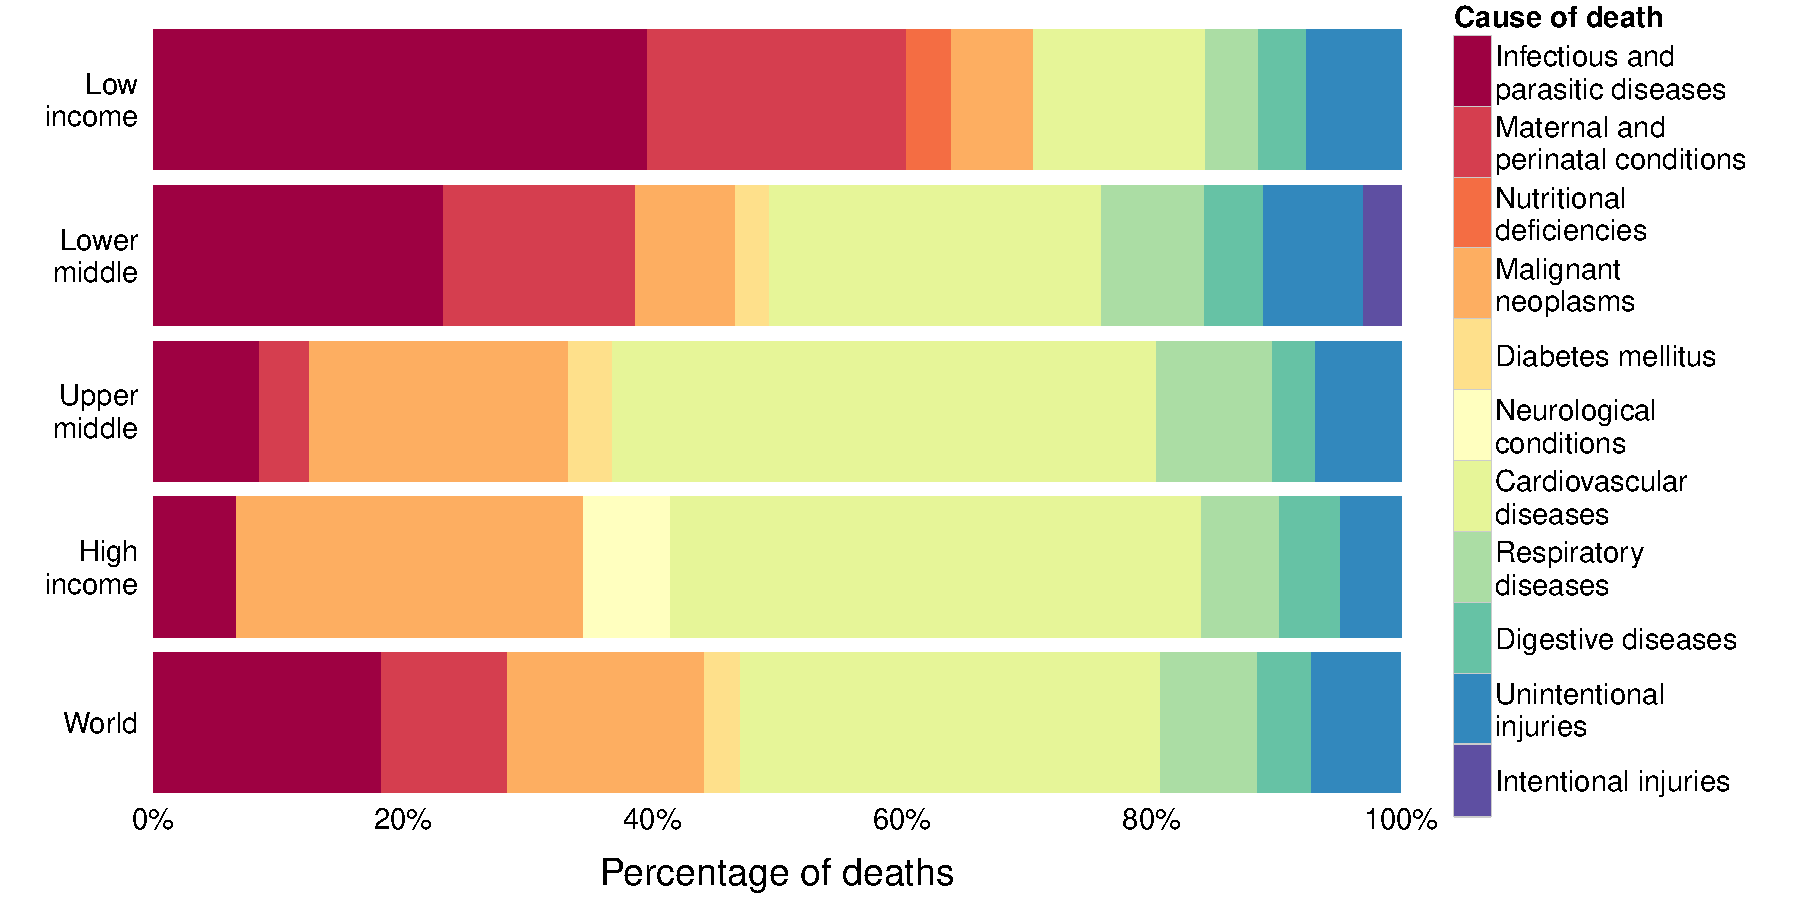
\includegraphics[width=\maxwidth]{figures/R/who-deaths/topCauses-who-deaths_top-causes-1} \caption[Relative frequencies of death causes in 2012 by World Bank income groups]{Relative frequencies of death causes in 2012 by World Bank income groups. Binning is based on Gross National Income (GNI) per capita and the thresholds are \$1'045 or less for low income, \$1046 to \$4125 for lower-middle, \$4126 to \$12745 for upper-middle and \$12746 or more for high income economies. The data was obtained from the \cite{WHO2012}.}\label{fig:who-deaths_top-causes}
\end{figure}


\end{knitrout}

\newcommand{\knitrTotalDeathsTwelve}{58.3 million}

\newcommand{\knitrPercentageDeathsTwelveHigh}{20.1\%}
\newcommand{\knitrPercentageDeathsTwelveLow}{14\%}
\newcommand{\knitrPercentageDeathsTwelveLmid}{36.5\%}
\newcommand{\knitrPercentageDeathsTwelveUmid}{29.4\%}

\newcommand{\knitrPercentDeathsTwelveLowInfect}{39.6\%}
\newcommand{\knitrPercentDeathsTwelveLowPerinat}{20.8\%}
\newcommand{\knitrPercentDeathsTwelveLmidInfect}{23.3\%}
\newcommand{\knitrPercentDeathsTwelveLmidCardio}{26.5\%}
\newcommand{\knitrPercentDeathsTwelveUmidInfect}{8.5\%}
\newcommand{\knitrPercentDeathsTwelveHighInfect}{6.7\%}
\newcommand{\knitrPercentDeathsTwelveWorldInfect}{18.3\%}
\newcommand{\knitrPercentDeathsTwelveWorldCardio}{33.7\%}


Despite development of means to treat and prevent many previously devastating diseases, infectious pathogens remain a serious threat to global health. In 2012, an estimated total of \knitrTotalDeathsTwelve{} people died (\knitrPercentageDeathsTwelveHigh{} in high, \knitrPercentageDeathsTwelveUmid{} in upper-middle, \knitrPercentageDeathsTwelveLmid{} in lower-middle and \knitrPercentageDeathsTwelveLow{} in low income countries). Figure \ref{fig:who-deaths_top-causes} partitions the total death count into World Bank income groups and causes. In low income countries, infective diseases are the most prevalent cause of death (\knitrPercentDeathsTwelveLowInfect{}), followed by maternal and perinatal complications with substantial margin (\knitrPercentDeathsTwelveLowPerinat{}). In lower middle income countries, cardiovascular conditions catch up (\knitrPercentDeathsTwelveLmidCardio{}), but are still almost matched in frequency by infectious diseases (\knitrPercentDeathsTwelveLmidInfect{}). In upper middle (\knitrPercentDeathsTwelveUmidInfect{}) and high income countries (\knitrPercentDeathsTwelveHighInfect{}), the importance of infectious disease while weakened remains accountable for a significant number of deaths. Globally, infectious diseases are the second most frequent cause of death (\knitrPercentDeathsTwelveWorldInfect{}), even more prevalent than all forms of cancer combined (\knitrPercentDeathsTwelveWorldCancer{}) and only preceded by cardiovascular diseases (\knitrPercentDeathsTwelveWorldCardio{}).

\begin{knitrout}
\definecolor{shadecolor}{rgb}{0.969, 0.969, 0.969}\color{fgcolor}\begin{figure}
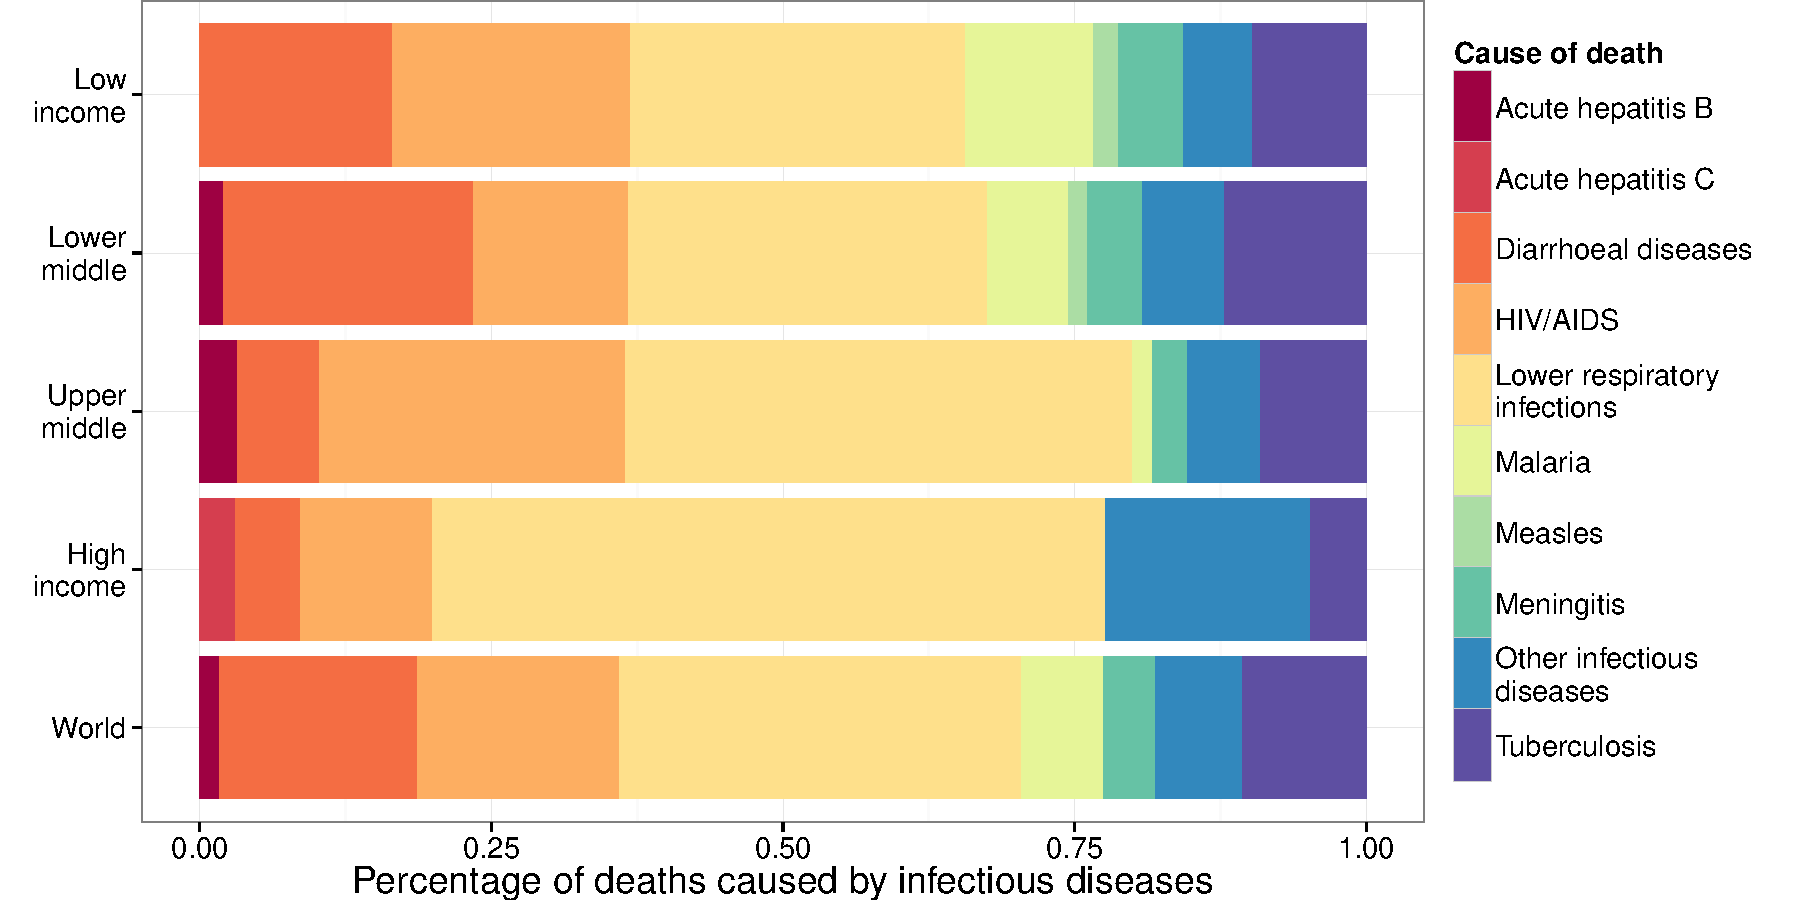
\includegraphics[width=\maxwidth]{figures/R/who-deaths/byDisease-who-deaths_by-disease-1} \caption[Relative frequencies deadly infectious diseases for 2012 by World Bank income groups]{Relative frequencies of deadly infectious diseases for 2012 by World Bank income groups. Binning is based on Gross National Income (GNI; see figure \ref{fig:who-deaths_top-causes}). The data was obtained from the \cite{WHO2012}.}\label{fig:who-deaths_by-disease}
\end{figure}


\end{knitrout}

\newcommand{\knitrPercentageInfectTwelveWorldLRI}{34.5\%}
\newcommand{\knitrPercentageInfectTwelveHighLRI}{57.7\%}
\newcommand{\knitrPercentageInfectTwelveUmidLRI}{43.5\%}
\newcommand{\knitrPercentageInfectTwelveLmidLRI}{30.8\%}
\newcommand{\knitrPercentageInfectTwelveLowLRI}{28.7\%}
\newcommand{\knitrPercentageInfectTwelveHighDiarr}{5.6\%}
\newcommand{\knitrPercentageInfectTwelveUmidDiarr}{7\%}
\newcommand{\knitrPercentageInfectTwelveLmidDiarr}{21.4\%}
\newcommand{\knitrPercentageInfectTwelveLowDiarr}{16.6\%}
\newcommand{\knitrPercentageInfectTwelveWorldAIDS}{17.3\%}
\newcommand{\knitrPercentageInfectTwelveWorldDiarr}{16.9\%}
\newcommand{\knitrPercentageInfectTwelveHighAIDS}{11.3\%}
\newcommand{\knitrPercentageInfectTwelveUmidAIDS}{26.2\%}
\newcommand{\knitrPercentageInfectTwelveLmidAIDS}{13.3\%}
\newcommand{\knitrPercentageInfectTwelveLowAIDS}{20.4\%}


Focusing only on deaths caused by infectious disease, lower respiratory infections are most frequent (for each income region individually, low to high: \knitrPercentageInfectTwelveLowLRI{}, \knitrPercentageInfectTwelveLmidLRI{}, \knitrPercentageInfectTwelveUmidLRI{} and \knitrPercentageInfectTwelveHighLRI{} as well as worldwide: \knitrPercentageInfectTwelveWorldLRI{}; cf. figure \ref{fig:who-deaths_by-disease}). Diarrhoeal diseases and \cgls{hiv}\slash \cgls{aids} are the next most common worldwide (\knitrPercentageInfectTwelveWorldDiarr{} and \knitrPercentageInfectTwelveWorldAIDS{}, respectively) where diarrhea is more prevalent in lower income regions (\knitrPercentageInfectTwelveLowDiarr{} and \knitrPercentageInfectTwelveLmidDiarr{} versus \knitrPercentageInfectTwelveUmidDiarr{} and \knitrPercentageInfectTwelveHighDiarr{}), while \cgls{hiv}\slash \cgls{aids} plays a major role irrespective of income region (low to high: \knitrPercentageInfectTwelveLowAIDS{}, \knitrPercentageInfectTwelveLmidAIDS{}, \knitrPercentageInfectTwelveUmidAIDS{} and \knitrPercentageInfectTwelveHighAIDS{}).

Dealing with highly virulent pathogens and preventing their spreading requires a multi-pronged approach. First and foremost, etiology and routes of transmission have to be understood. Knowledge of vectors and natural reservoirs is of great importance as a first line of defense. In the case of plague, for example, insecticides killing fleas were successfully used as a prophylactic measure, as was controlling rat populations \citep{Barnes1990}. Sanitary precautions including purification of drinking water, cocking foods well and the usage of disinfectants prevent initial infection, while measures such as sewage treatment, hand washing and wearing face masks help limiting spread among humans. Vaccination is the most important preventive measure. Exposing the immune system to a foreign antigen in a controlled manner artificially induces immunity. Among the great successes of widespread vaccination efforts is the global eradication of smallpox through a coordinated initiative lead by the World Health Organization in the 1970's.

Post-infection therapies include symptomatic treatments, as well as anti-in\-fec\-tive drugs. Antibiotics exploit differences in proteomes between host and pathogen to selectively disable the invader with minimal toxicity to the host. This approach has been tremendously successful throughout most of the 20th century, leading to widespread application and prompting development of resistance towards the commonly used compounds. Adding to the severity of the problem is a lack of discovery of new drugs. No new class of anti-bacterial agents has been found since 1987, causing big pharmaceutical companies to withdraw from the area. The remaining research is mainly focused on improving on existing drugs, leading to a weak product pipeline, especially for the treatment of gram-negative bacteria \citep{Silver2011}. In its first global study on anti-microbial resistance, the \citet{WHO2014} notes:

\begin{quote}
\cGls{amr} within a wide range of infectious agents is a growing public health threat of broad concern \ldots A post-antibiotic era—-in which common infections and minor injuries can kill—-far from being an apocalyptic fantasy, is instead a very real possibility for the 21st century.
\end{quote}

An alternative to pathogen directed search lies in targeting the set of host proteins necessary for infection. Many intracellular parasites subvert cellular functions to gain entry via host-mediated processes such as endocytosis. Upon entry, they move to a suitable niche and rely on host resources for proliferation. Challenges include evading host-cell defense mechanisms, generating sufficient space for replication, nutrient acquisition and keeping the host alive as long as possible, most of which require complex interactions between invader and host-based mechanisms. Finally, exiting the host cell again requires the parasite to successfully insert itself into existing signaling pathways \citep{Leiriao2004}.

\cGls{hdt} offer an escape from the conundrum of wanting to combat but not wanting to select for the surviving microbial parasites. The major challenge under this regimen is finding infectome components that are nonessential for cell survival, as orthogonality of host and infectant can no longer be exploited. Proving feasibility of the approach, \citeauthor{Czyz2014} screened a library of 640 compounds already approved by the United Stated Food and Drug Administration (USFDA or short FDA) for inducing resistance to four intracellular pathogens (\textit{Coxiella burnetii}, \textit{Legionella pneumophila}, \textit{Brucella abortus}, and \textit{Rickettsia conorii}). They found multiple drugs, not classified as antibiotics, that successfully inhibited intracellular bacterial growth while entailing only limited toxicity to THP-1 host cells. \citeauthor{Prussia2011} review the usage of genome-wide screens to study host-pathogen interactions (for \cgls{hiv} and influenza) which in turn serve as basis for rational identification of drug targets for novel host-directed antivirals. \nocite{Hawn2015}

A detailed understanding of the human infectome is of crucial importance to the development of \cgls{hdt} and may even benefit the development of new anti-microbial agents. Feasibility of systematic loss of function screens using \cgls{rna} interference methodology offers a unique opportunity to investigate complex cellular networks, making this an ideal tool for laying groundwork in combating infectious diseases. Of great importance, however, is ensuring reproducibility and comparability of such datasets, as well as ready availability to the scientific community.

Created to tackle such issues, InfectX and TargetInfectX are two successive \cgls{rtd} projects funded by SystemsX, the Swiss initiative for systems biology, contracted with identification and study of the human infectome for a set of bacterial (\textit{Bartonella henselae}, \textit{Brucella abortus}, \textit{Listeria monocytogenes}, \textit{Salmonella} typhimurium and \textit{Shigella flexneri}) and viral pathogens (adenovirus, rhinovirus and \textit{Vaccinia virus}). The central effort of generating kinome- and genome-wide \cgls{sirna} screens for each of the investigated pathogens and capturing image data followed by computational image analysis is carried out by an interdisciplinary consortium of research groups spanning the Universities of Basel and Z\"urich, the Swiss Federal institute of Technology (ETH Z\"urich), as well as the Pasteur Institute.

A wealth of data is easily generated by running computational feature recognition at single cell resolution on microscopic images which subsequently calls for sophisticated statistical analysis in order to expose biologically relevant information. This master thesis explores the single cell feature space, provides software to handle such datasets and attempts to employ \cglspl{glm} for comparing \cgls{sirna}-knockdown experiments and identifying discriminatory features. Following this introductory part, chapter 2 will provide the necessary biological background, covering microbial infection mechanisms, a description of each pathogen in terms of physical characteristics, diseases caused, pathogenesis and epidemiology, as well as giving an introduction on \cgls{rna} interference, including molecular mechanism, biological function and several applications alongside methodological caveats. Chapter 3 reviews InfectX data collection, detailing experimental setup, image acquisition, data processing and image analysis, as well as qualitatively describing the available datasets.

An R package called singleCellFeatures was developed to facilitate working with single cell feature datasets, the specifics of which are detailed in chapter 4. Beginning with a motivational example, the importance of efficient computation and data representation is highlighted and the R package is described in terms of developed S3 classes as well as data fetching, caching, manipulation and analysis routines. Finally, chapter 5 introduces \cglspl{glm}, \cglspl{pmm}, deliberates several normalization approaches and concludes with some analysis results along with a discussion of unresolved issues.


\chapter{Biological Background}

In order to better understand infectious diseases from a cell biological standpoint, this chapter reviews the current state of knowledge surrounding both bacterial and viral entry mechanisms. A sweeping overview of epidemiology and pathogenesis for several specific bacterial (\textit{Bartonella henselae}, \textit{Brucella abortus}, \textit{Listeria monocytogenes}, \textit{Salmonella enterica} and \textit{Shigella flexneri}), as well as viral parasites (adenoviruses, rhinoviruses and \textit{Vaccinia virus}) is given and the chapter concludes with a look at RNA interference as this mechanism is a cornerstone of genome-wide knockdown experiments.

\section{Microbial Host-Cell Infection}

Multi-layered keratinized skin is impenetrable for almost all microbial parasites. Instead they either require breaches such as cuts, scratches, puncture wounds and arthropod bites, or environmental interfaces which offer less impervious protection. Examples include respiratory, gastrointestinal and urogenital tracts, which all contain segments where only a single layer of epithelial cells has to be overcome. Although often protected by chemical defense mechanisms (acidity of the stomach and urogenital tract, as well as microbicidal factors in mucous secretions in the respiratory tract and small intestine), combined with frequent flushing (urination, peristalsis and the coordinated beating of cilia), some microbes have adapted to survive these hostile environments.

For extracellular pathogens to successfully colonize epithelial linings, they must avoid being removed by cleansing mechanisms of the host. Many bacteria accomplish this by expressing adhesins, protein complexes that recognize and bind to specific host-cell receptors, providing host and tissue tropism. Bacterial pili serve to extend reach and penetrate mucous secretions and therefore often carry adhesins. Enteropathogenic \textit{Escherichia coli} have extended this scheme by injecting their own receptor protein \glsrev{tir} through the \glsrev{t3ss} into the host cell to which it then attaches. This has the additional advantage that the intracellular domain of \gls{tir} can be used to modify host cell behavior \citep{Alberts2008}.

The outside of many epithelial barriers is covered in natural bacterial flora and crossing over into sterile cavities has the advantage of not having to compete with organisms well accustomed to that particular niche. Furthermore, intracellular pathogens are no longer accessible to antibodies and phagocytic cells and have a nutrient rich environment at their disposal. Mechanisms for entering host cells are described in the following sections.

\subsection{Viral Infection Mechanisms}

The first step of any viral entering sequence is binding to the target surface. This can be mediated by attachment factors which simply serve to concentrate the virions on the cell membrane or by virus receptors, which additionally act as communicators between host and pathogen. Common attachment factors include glycosaminoglycan chains and sialic acids and are comparatively unspecific. Glycoprotein spikes on enveloped and capsid proteins of non-enveloped viruses provide host specificity by binding cellular receptors. Mostly these cellular receptors serve other purposes which are exploited for infection. Binding affinity for individual interactions may be weak but aggregation of multiple interactions provide virtually irreversible avidity \citep{Smith2012}.

\paragraph{Viral import.}
For viral cell entry, different strategies exist. Enveloped viruses can either directly fuse with the plasma membrane (e.g. \gls{hiv}) or be endocytosed by the host cell (e.g. influenza), while non-enveloped viruses either create a pore and directly inject their genome into the cytosol (e.g. polio virus) or are endocytosed (e.g. adenovirus). Endocytosis has major advantages over alternative strategies. Reaching its replicatory niche within the host cell is a difficult task for a microorganism having no means of locomotion and hijacking the endocytic system solves this problem elegantly. Furthermore, maturation of endosomes provides precise environmental cues to the invader for triggering uncoating and release. Both fusion with the cell membrane and injection of viral material into the cytosol leaves back traces of infection to be detected by the immune system. Being completely engulfed by the host, however, the intruders leave back no telltale traces. Additionally, lytic membrane penetration techniques are not as problematic to the host if only applied inside an endosome as opposed to the plasma membrane.

Endocytic viruses trigger uptake either in a receptor mediated fashion (clathrin, caveolin or lipid raft dependent) or via non-specific macropinocytosis. The clathrin pathway is most widely used, for example by rhinoviruses, some adenoviruses, and coronaviruses and presents with characteristic invaginations, termed \glspl{ccp}. The inwards facing pockets are subsequently pinched off by the membrane scission proteins dynamin-1 and dynamin-2, releasing clathrin-coated vesicles into the cytosol. Caveolin-mediated endocytosis is though to be a more tightly regulated and low capacity pathway but is nevertheless exploited by several virus species, including picornaviruses and some retroviruses. Caveola formation is lipid raft dependent and recruitment of caveolin yields 50--70 nm flask-shaped pockets which are closed off by dynamin action. A lipid raft dependent, caveolin independent pathway has been described in simian virus 40 infection, but remains poorly understood. Lastly, larger virions such as poxviruses or herpesviruses initiate macropinocytosis, a mechanism typically employed by the cell for non-specific uptake of extracellular particles. An actin dependent membrane ruffling leads to formation of a lamellipodium which folds back onto the plasma membrane, enclosing an extraluminal volume and thus creating a macropinosome.

\begin{figure}
  \centering
  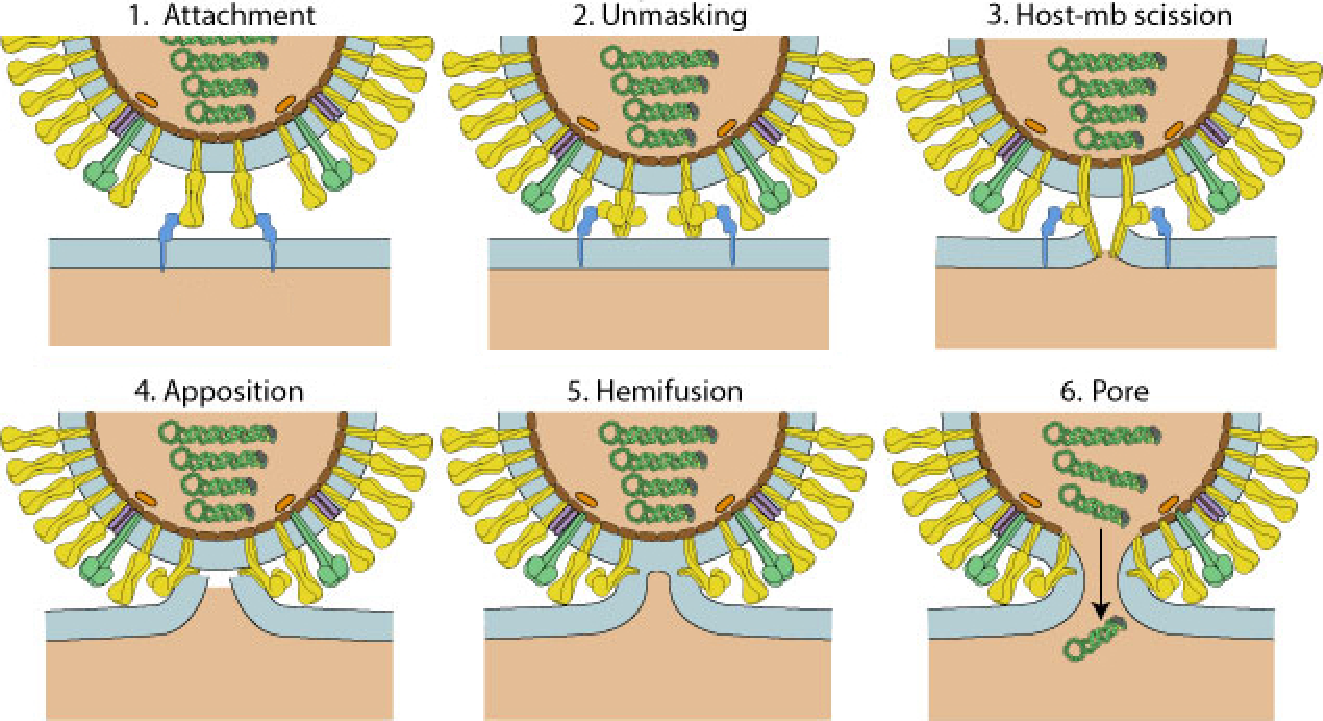
\includegraphics[width=0.95\textwidth]{virus-membrane-fusion}
  \caption[A generalized view of the steps necessary for viral--cellular membrane fusion]{A generalized view of the steps necessary for viral--cellular membrane fusion. In pre-fusion conformation, fusion proteins have their hydrophobic fusion moieties tucked away. Upon attachment (1), they are unmasked (2), interact with the target membrane and ultimately penetrate it. Conformational change in fusion proteins induces membrane scission (3) and forces the two bilayers into close proximity (4), yielding a state of hemifusion (5). Finally a fusion pore is formed (6), stabilized by the post-fusion conformation which is lower in energy than the pre-fusion state. Adapted from \cite{Hulo2011}}
  \label{fig:virus-membrane-fusion}
\end{figure}

Upon endocytic uptake, viral pathogens need to uncoat and eject their genetic material into the cytosol, as soon as their replicatory niche is reached. Escape timing is a critical issue, as late endosomes finally turn into lysosomes, capable of digesting their contents. Many enveloped viruses employ fusion mechanisms, which can be classified as type I or type II. For both types, increasing acidity associated with endosome maturation, initiates membrane fusion. Type I fusion proteins are forced into a metastable conformation prior to being added to the viral envelope and low pH triggers a conformational change to a state of lower energy. The energy released is used to force the two membranes close together resulting in their fusion (see figure \ref{fig:virus-membrane-fusion}). In type II fusion proteins, the critical transformation is not a conformational change but one in quaternary structure.

Non enveloped viruses cannot fuse with host membranes and have developed alternative approaches such as lysis (e.g. adenovirus) or ejecting their genome through pore-forming complexes (e.g. reovirus). Polyomaviruses need to pass through the \gls{er} because they rely on \gls{er} localized proteins to uncoat their capsid. For export from the \gls{er} into the cytosol, they exploit the \gls{erad} pathway, which serves as export mechanism for misfolded proteins from the endoplasmic reticulum to be degraded by proteasomes.

\renewcommand{\arraystretch}{1.5}

\begin{table}
  \centering
  \caption[The Baltimore classification scheme for viruses]{The Baltimore classification scheme is based on diversity of genetic system that have evolved in viruses. For each group, a selection of virus families capable of infecting humans, is provided, along with whether the virions are enveloped and the location of their replicatory niche. The data was obtained from \cite{Hulo2011}}
  \label{tab:baltimore-classification}
  \footnotesize
  \begin{tabular}{c|l|l|c|c}
    & Genome based class & Examples & Enveloped & Replication site \\
    \hline \multirow{4}{*}{\begin{sideways}DNA viruses\end{sideways}} &
    \multirow{2}{*}{Group I: dsDNA} &
    \textit{Adenoviridae} &
    no & nucleus \\
    \cline{3-5} &
    & \textit{Poxviridae} &
    yes & cytoplasm \\
    \cline{2-5} &
    \multirow{2}{*}{Group II: ssDNA(+)} &
    \textit{Parvovirinae} &
    no & nucleus \\
    \cline{3-5} &
    & \textit{Anelloviridae} &
    no & nucleus \\
    \hline \multirow{6}{*}{\begin{sideways}RNA viruses\end{sideways}} &   
    Group III: dsRNA &
    \textit{Reoviridae} &
    no & cytoplasm \\
    \cline{2-5} &
    \multirow{3}{*}{Group IV: ssRNA(+)} &
    \textit{Coronaviridae} &
    yes & cytoplasm \\
    \cline{3-5} &
    & \textit{Picornaviridae} &
    no & cytoplasm \\
    \cline{3-5} &
    & \textit{Hepeviridae} &
    no & cytoplasm \\
    \cline{2-5} &
    \multirow{2}{*}{Group V: ssRNA(-)} &
    \textit{Filoviridae} &
    yes & cytoplasm \\
    \cline{3-5} &
    & \textit{Paramyxoviridae} &
    yes & cytoplasm \\
    \hline \multirow{2}{*}{\begin{sideways}Retro\end{sideways}} &   
    Group VI: ssRNA(+)-RT &
    \textit{Orthoretrovirinae} &
    yes & nucleus \\
    \cline{2-5} &
    Group VII: dsDNA-RT &
    \textit{Hepadnaviridae} &
    yes & nucleus
  \end{tabular}
\end{table}

\paragraph{Replication.}
In contrast to larger intracellular parasites that carry the genetic information required for sustaining their own metabolism and replication, viral pathogens typically rely almost exclusively on host machinery. Furthermore, viruses have developed strategies for interfering with host transcription and translation in order to promote synthesis of viral proteins at the expense of host gene expression. Even modulation of the host cell cycle is not uncommon, as some DNA viruses (including adenoviruses) are able to trigger a G1 to S phase transition, yielding an increased concentration of active DNA polymerase, while other species are capable of inducing a G2/M arrest, which again provides an optimized environment for those viruses. Further virus--host interactions include regulation of apoptosis, immune response modulation and interferon signaling.

The remarkable diversity of genomic systems employed by viruses is captured by a classification system devised by \cite{Baltimore1971}. Table \ref{tab:baltimore-classification} lists the 7 types of viral genomes alongside examples of human viruses for each group, as well as whether those viruses are enveloped and where they replicate. Consequently, requirements for replication, transcription and translation vary widely among the different groups of viruses and due to the resulting mechanistic heterogeneity, viral propagation is not further explored within this general section. An excellent overview is provided by the online database of \citeauthor{Hulo2011}.

\paragraph{Viral export.}
The final stage of the viral life-cycle is concerned with virion assembly and exiting the host cell. Again, many strategies exist. Some nuclear replicating viruses (such as polyomaviruses) assemble their capsid proteins within the nucleus, requiring their structural proteins to target the nucleus via \glspl{nls} and leave the nucleus by disrupting the nuclear envelope, while others have their genome exported via nuclear pores and assemble progeny virions in the cytoplasm. Some cytoplasmic viruses (including poxviruses) replicate within special structures called viral factories or viroplasms, which increase efficiency of assembly and packaging and provides protection from host defense mechanisms. Other cytoplasmic viruses localize to organelles such as the \gls{er} (e.g. flaviviruses) where they are assembled and enter the secretory pathway via the Golgi apparatus. For intracellular motility, large virions such as poxviruses or herpesviruses have to rely on microtubule dependent transport whereas particles smaller than 20 nm can freely diffuse within the cytosol.

Once the host cell resources are depleted and replication is completed, progeny virions trigger their release. Viral shedding may occur via cell lysis, apoptosis, exocytosis or virion budding. Most non-enveloped and few enveloped viruses disrupt the plasma membrane with lytic viroproteins leading to cell death and release of cytoplasmic contents. While many viruses inhibit  apoptosis, typically employed as a host defense measure, some (including hepeviruses and lentiviruses) have been implicated in exploiting this mechanism for expulsion and possibly subsequent infection of macrophages. Exocytosis and virion budding are two release strategies that are non-lethal to the host cell. Enveloped viruses acquire host-derived membrane either within the cell, typically at \gls{er} or Golgi exit sites or directly from the plasma membrane. In the latter case, envelopment coincides with host exit, whereas in the former case, virions are expelled via fusion of exocytic vesicles with the plasma membrane.

\subsection{Bacterial Entry Mechanisms}

Due to the much larger size of bacterial pathogens, endocytosis is not a feasible mechanism for entry. Phagocytosis, however can deal with uptake of particles this large. While phagocytosis is a function usually only available to macrophages, some bacteria have evolved mechanisms of inducing phagocytosis in other cell types. Species explicitly targeting macrophages, such as \textit{Mycobacterium tuberculosis} and \textit{Legionella pneumophila}, have to be able to escape phagosomes or deal with resisting digestion.

Two recurring patterns for inducing phagocytosis in non-phagocytic cells have been described as the zipper mechanism, encountered in \textit{Yersinia pseudotuberculosis} and \textit{Listeria monocytogenes} and the trigger mechanism used by \textit{Salmonella enterica} and \textit{Shigella flexneri}. Not all entry strategies can be assigned to these two classes and several additional, unrelated pathways have been investigated.

\begin{figure}
  \centering
  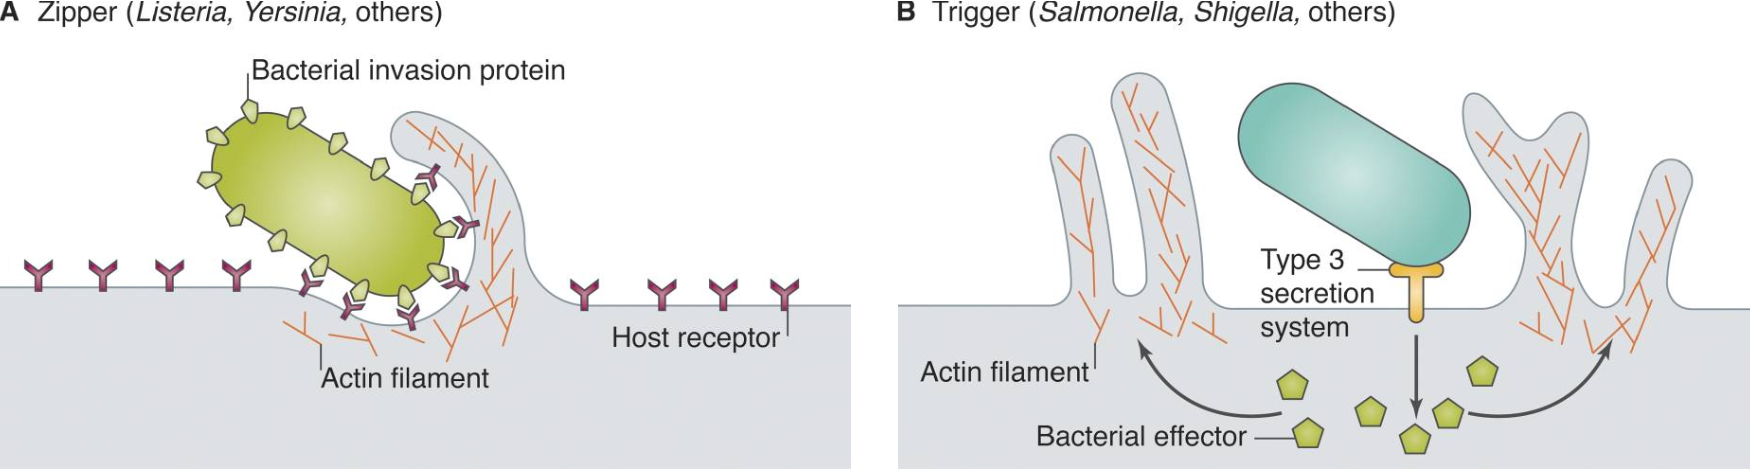
\includegraphics[width=0.6\textwidth]{zipper-trigger}
  \caption[Zipper and trigger mechanisms for bacterial host-cell entry]{Both the zipper (A) and trigger mechanisms (B) are actin dependent and lead to phagocytosis by usually non-phagocytic host cells. Zippering bacteria display an invasion protein on their surface that recruits actin filaments via a host receptor, while triggering bacteria inject an effector into the host cytosol via a type III secretion system leading to uptake. \citep{Haglund2011}}
  \label{fig:zipper-trigger}
\end{figure}

\phantomsection
\label{zipper-mechanism}

\paragraph{Zipper Mechanism.}
The first step for zippering bacteria is binding to target cell receptors by expressing adhesins. \textit{Y. pseudotuberculosis} displays invasins on its cell surface, capable of interacting with \textbeta$_1$ integrins, while \textit{L. monocytogenes} uses internalin A, a protein that binds E-cadherin. In both settings, a downstream signaling cascade leads to actin polymerization via recruitment of an \glsrev{arp-2-3} complex and \glsrev{rac-1}, yielding a phagocytic cup.

Cadherin and integrins are usually involved in anchoring cell junctions and the host cell is fooled into thinking, a neighboring cell is initiating formation of such a junction. Responding by recruiting actin at the site of bacterial attachment to cover the surface of mistaken invasion proteins leads to engulfment and phagocytosis to the bacterium. This process incurs only modest cytoskeletal rearrangements. 

\phantomsection
\label{trigger-mechanism}

\paragraph{Trigger Mechanism.}
In case of the trigger mechanism, bacterial \gls{t3ss} weakly adhere to target cell receptors (CD44 for \textit{Shigella}) and effector molecules are injected into the host cytosol through a pore formed by \glsrev{sip} or \glsrev{ipa} proteins. These induce major actin rearrangements that result in localized ruffling of the plasma membrane and subsequent swallowing of the bacterium.

Early in \textit{Shigella} entry, VirA, secreted through the \gls{t3ss} causes local destabilization of microtubules by binding to \textalpha/\textbeta-tubulin heterodimers. This in turn stimulates \glsrev{rac-1} activity, \glsrev{cdc-42} recruitment and subsequent \gls{arp-2-3} activation leading to protrusions formed by actin filaments. \Gls{ipa}C recruits the Src tyrosine kinase further enhancing actin dynamics. Upon closing of the phagocytic pocket, the \gls{t3ss}-secreted protein \gls{ipa}A binds to vinculin and induces actin depolymerization.

\textit{Salmonella} inject the proteins \glsrev{sop}E and \glsrev{spt-p}, an activator/inhibitor pair for the GTPase complex \gls{rac-1}/\gls{cdc-42}, into the host cell. First, \gls{gef} activity of \gls{sop}E induces massive actin-rearrangements leading to membrane ruffling and facilitating phagocytosis, followed by GAP activity of \gls{spt-p}, restoring the inactive \gls{gdp} state of \gls{rac-1}/\gls{cdc-42} and leading to actin depolymerization. \Gls{sop}E is degraded more rapidly than \gls{spt-p}, enabling the invading pathogen to reversibly control the pathways exploited for entering.

\paragraph{Other Entry Pathways.}
In addition to trigger and zipper type uptake, other atypical mechanisms exist. Host cell entry of \textit{Brucella abortus}, for example, has been described as invasome mediated \citep{Dehio2005}. In this actin dependent process, bacteria aggregate on the cell surface and trigger their engulfment by injecting bacterial effectors into the host via \gls{t4ss}. The internalized structure is called an invasome. Actin-independent uptake albeit rare, is possible as evidenced by \textit{Campylobacter jejuni}, which have evolved a microtubule dependent invasion strategy \citep{Kopecko2001}.

\subsection{Actin-based Intracellular Motility}
\label{subsec:actin-motility}
As for large viruses, free diffusion within the cytoplasm is not possible for bacteria.

\section{Select Bacterial Pathogens}

A total of 5 bacterial pathogens were selected for study within the InfectX RTD project by SystemsX. This section shortly describes each organism in terms of microbiological features, pathogenesis, epidemiology and diseases caused in humans. For each organism, a chapter of \cite{Rolain2006} serves as basis and is augmented by one or two review article referenced in the first paragraph of each section.

\subsection{\textit{Bartonella Henselae}}

\textit{Bartonella henselae} is a short, rod shaped, unflagellated proteobacterium, phylogenetically closely related to the genus \textit{Brucella}, presenting 94.4\% 16S rRNA gene sequence homology, compared with \textit{Brucella abortus}. The Gram-negative bacillus is a facultative anaerobic, intracellular parasite and was first described in 1992. Relatively harmless for healthy humans, infections can become life threatening in immunocompromised patients, making the species an important opportunistic pathogen \citep{Anderson1997}.

\paragraph{Diseases.}
In immunocompetent humans, infection with \textit{B. henselae} can lead to a condition known as \gls{csd}. As the name suggests, most patients report being in contact with a cat and transmission often occurs through scratches and bites. Affecting primarily children and young adults (80\% are 21 or younger), the self limiting infection typically presents itself with lymphadenopathy. Most patients remain afebrile and do not report feeling ill, with low-grade fever and malaise shown in roughly 30\% of the cases. Recovery from uncomplicated \gls{csd} usually takes 2 to 6 months and requires no specific treatment.

Possible complications include Parinaud's oculoglandular syndrome (granulomatous conjunctivitis in one eye and parotid lymphadenitis on the same side), splenomegaly and hepatic or splenic abscesses, accompanied by fever, weight loss, fatigue and malaise. In 1 to 7\% of the cases, the disease spreads to the central nervous system, leading to encephalopathy, but recovery is usually rapid (within several weeks).

Infections with \textit{B. henselae} tend to have more severe consequences for immunocompromised patients, such as bacillary angiomatosis, bacteremia and endocarditis. \Gls{aids} patients suffering from \gls{csd} usually experience severe, progressive disease with infection spreading systematically and without appropriate treatement, fatal outcome. \textit{Bartonella spp.} are the only prokaryotes known to be able to induce angiogenic tumors such as bacillary angiomas, which may involve skin, respiratory or gastrointestinal epithelia, hart, liver, spleen, bone marrow, muscles, or lymph nodes. Bacteremia may lead to inflamed heart valves, usually requiring endocarditic patients to have heart valve replacement surgery.

\begin{figure}
  \centering
  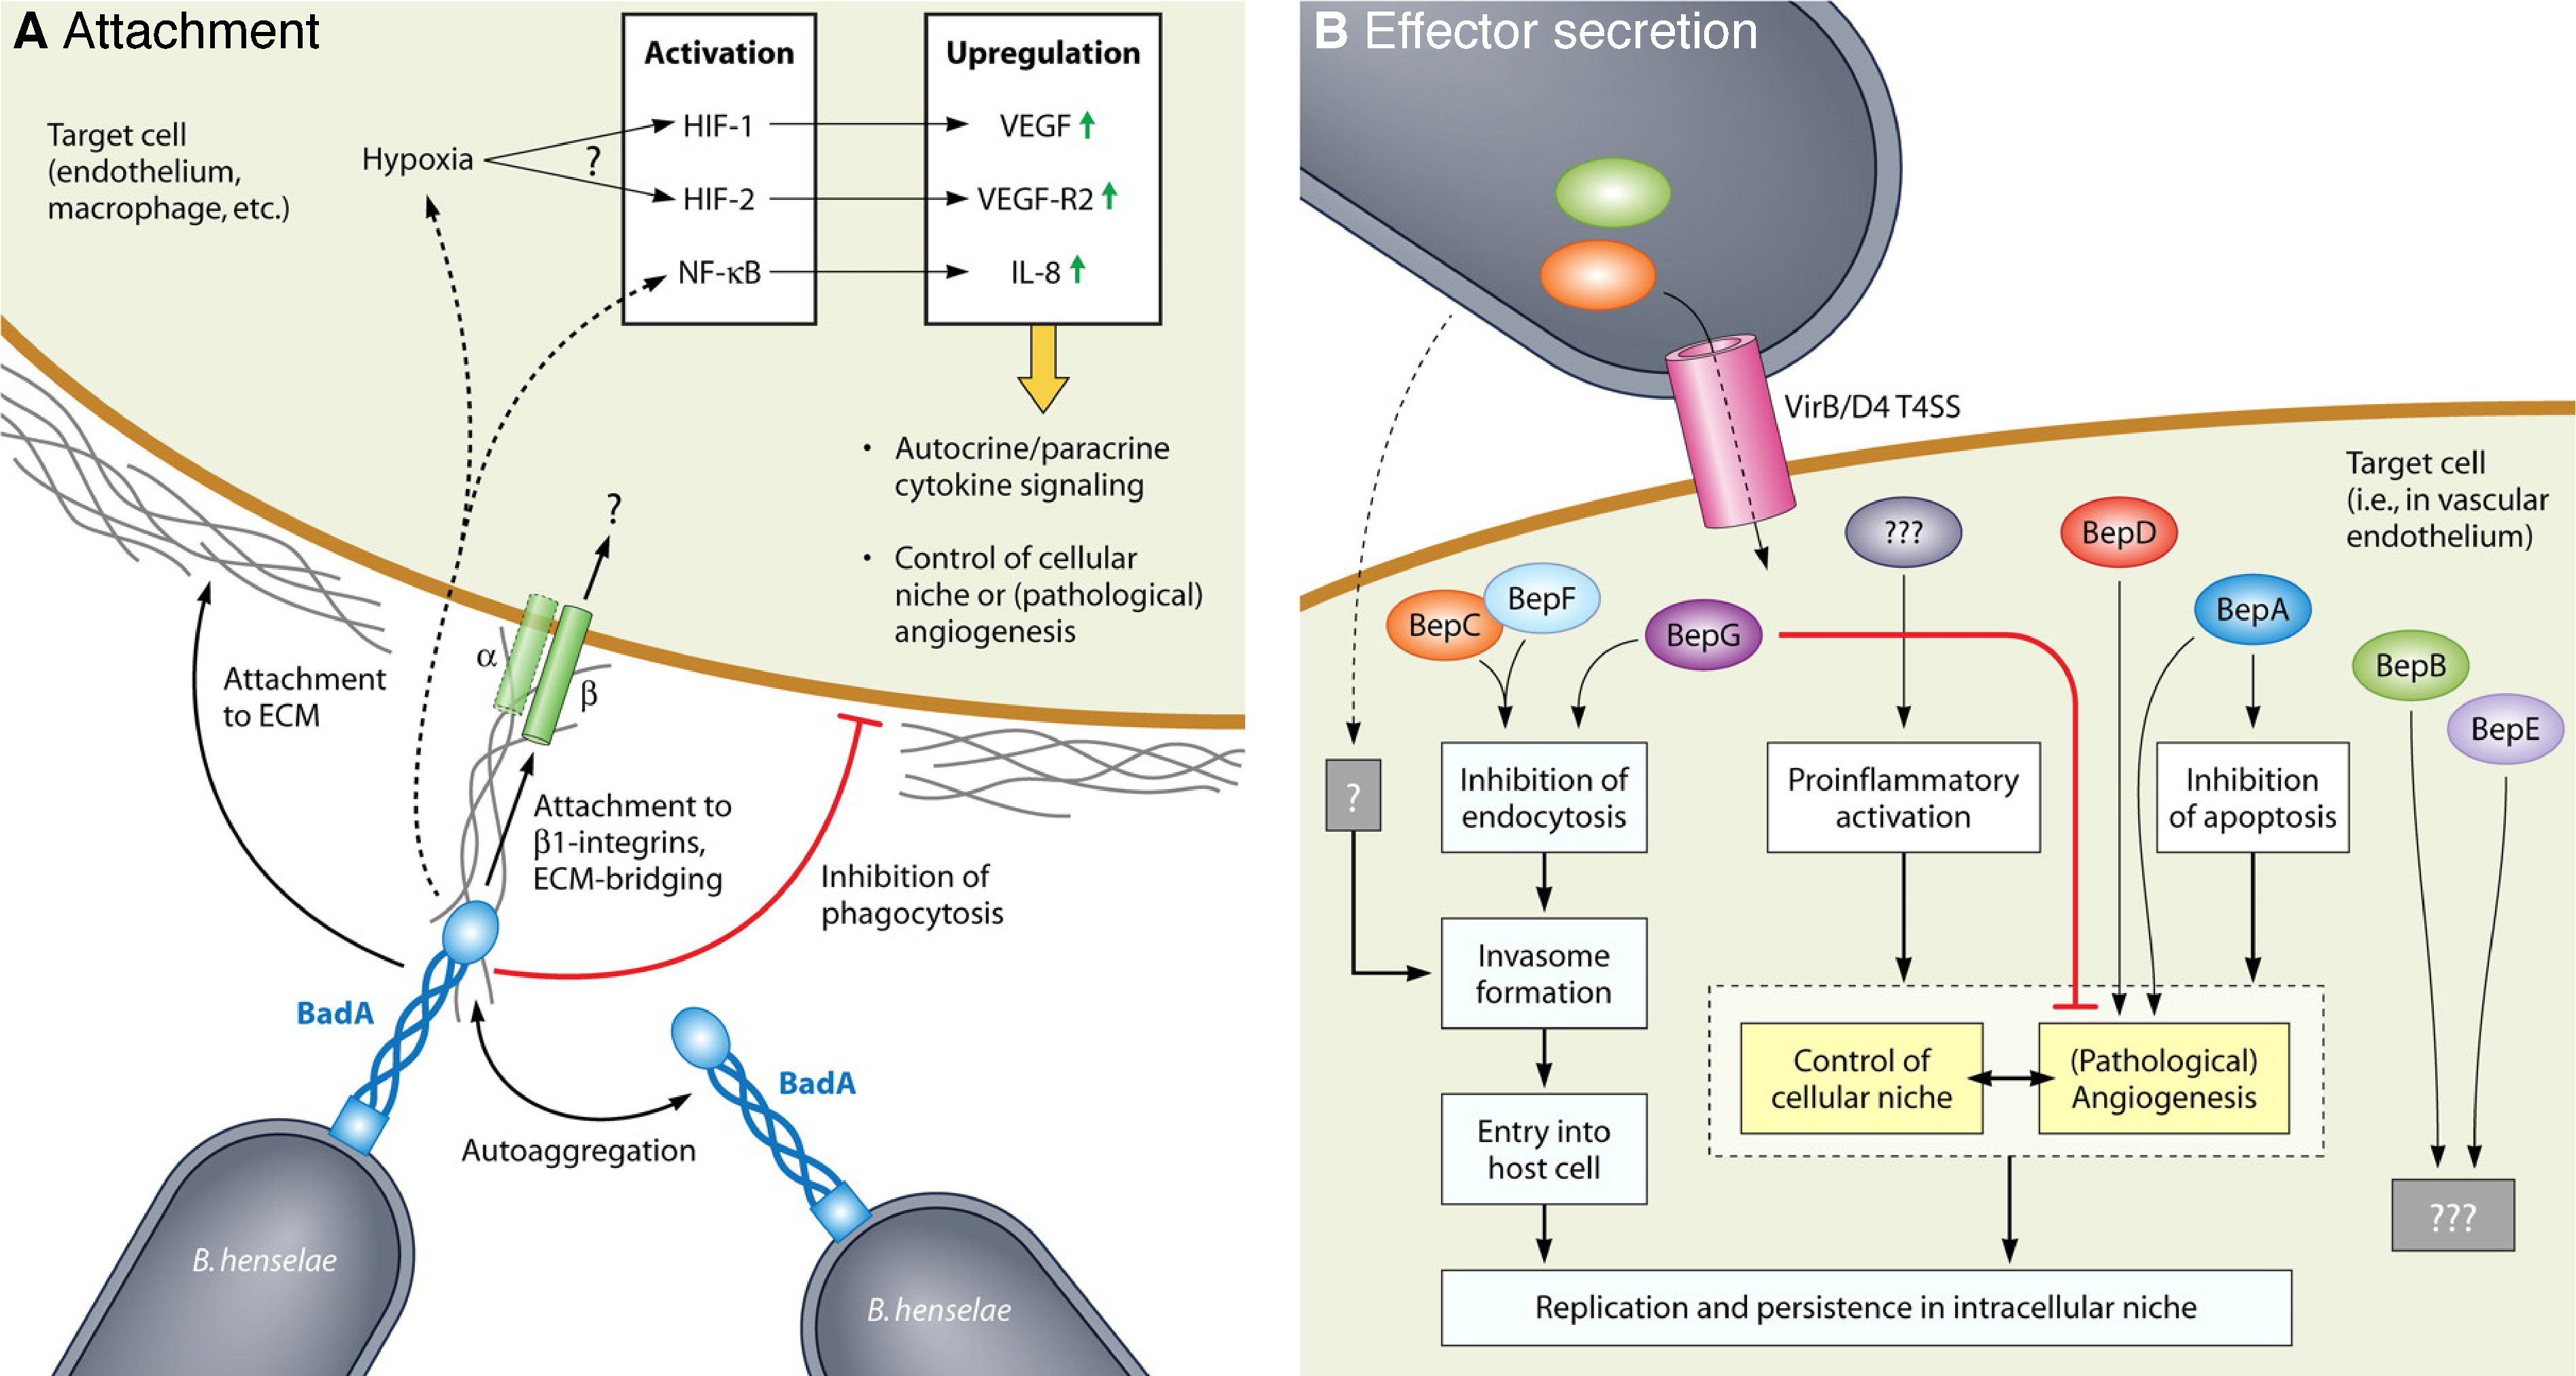
\includegraphics[width=0.75\textwidth]{bartonella}
  \caption[Replication cycle of \textit{Vaccinia viruses} for both intracellular mature and extracellular enveloped virions.]{Capsid proteins VP1 through VP4 form a pseudo $T=3$ icosahedral coat, roughly 30 nm in diameter around the RNA genome (A), which is monopartite, linear, 7.2 kp long and encodes 11 proteins \citep{Harms2012}.}
  \label{fig:bartonella}
\end{figure}

\paragraph{Pathogenesis.}
\textit{B. henselae} are capable of intracellular growth in both epithelial cells, and erythrocytes. Bundle forming type IV pili are essential for binding to target cells, making them important virulence factors. Internalization into red blood cells may be spectrin mediated and the bacterial protein deformin may also be involved. Endothelial receptors involved include \gls{icam-1} uptake is either via endocytosis or by a unique cellular structure termed an invasome.

Vasculogenesis is induced though an increased production in \gls{vegf} by infected host cells. Currently it is poorly understood how the pathogen provokes overexpression but the mechanism has been determined to be protease sensitive.

\paragraph{Epidemiology.}
The role of cats and in particular kittens, as reservoirs to \textit{B. henselae} has been firmly estabished. Infected felines are asymptomatic and show no signs of illness. Cat fleas (\textit{Ctenocephalides felis}) serve as vectors to spread the bacteria among cats and have also been suspected of infecting humans. The main path of transmission to humans however, is through scratches and bites by infected cats. \textit{B. henselae} has also been found in ticks and tick bites prior to contraction of \gls{csd} have been reported.

In the United States, 24000 cases of \gls{csd} are reported yearly, yielding 2000 hospital admissions with an estimated health care cost of \$12 million. Children are more likely to be affected (80\%) and incidence is higher in males (60\%). The seasonal pattern (occurrences higher in fall/winter) is attributed to cat mating patterns, as well as pet acquisition fluctuations.

\subsection{\textit{Brucella Abortus}}

The Danish physician David Bang first isolated \textit{Brucella abortus} in 1895 from cyetic cattle tissue, investigating a contagious disease causing abortions in cows. \textit{B. abortus} are small, unflagellated proteobacteria with a cell wall consisting of an outer layer of \gls{lps} (9 nm) and an inner layer of muramyl mucopeptide complexes (3--5 nm). The Gram-negative cocobacilli appear to have evolved from free-living, soil-dwelling species and are closely related to other human pathogens such as \textit{Bartonella} spp., based on 16S rRNA sequences. Brucella species were investigated for possible use as warfare agents in the mid 20th century by several armed forces. \citep{Atluri2011}

\paragraph{Diseases.}
Brucellosis is a human disease caused by several pathogenic \textit{Brucella} species, most importantly \textit{B. abortus}, \textit{B. melitensis}, \textit{B. canis} and \textit{B. suis}. Onset may be acute or insidious and due to protean symptoms, diagnosis based on clinical presentation alone is difficult. The febrile disease is generalized and may involve many parts of the body, including nervous, skeletal, gastrointestinal, cardiovascular, respiratory and genitourinary systems. Furthermore, as the bacteria spread to other reservoir hosts via their reproductive systems, persistence of infection is crucial to the pathogen and it comes as no surprise that brucellosis can manifest as a chronic disease in humans too.

Fever is the most consistent sign of \textit{Brucella} infection and depending on what specific organs are affected, further symptoms include asthenia, anorexia, nausea, malaise, arthritis, hepatomegaly, splenomegaly, epididymo-orchitis in males, and pulmonary manifestations such as bronchitis or pneumonia. A rare complication (less than 2\%), albeit the most lethal, is infective endocarditis. Invasion of the nervous system occurs in less than 5\% of cases and often results in meningitis or meningoencephalitis with good prognosis under antimicrobial treatment.

\begin{figure}
  \centering
  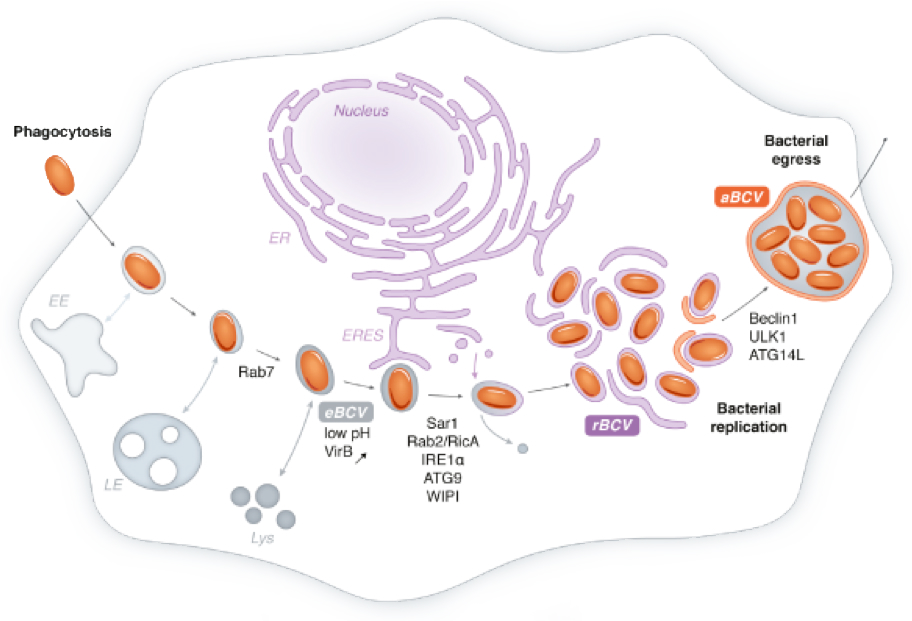
\includegraphics[width=0.95\textwidth]{brucella}
  \caption[Replication cycle of \textit{Vaccinia viruses} for both intracellular mature and extracellular enveloped virions.]{Capsid proteins VP1 through VP4 form a pseudo $T=3$ icosahedral coat, roughly 30 nm in diameter around the RNA genome (A), which is monopartite, linear, 7.2 kp long and encodes 11 proteins \citep{Celli2015}.}
  \label{fig:brucella}
\end{figure}

\paragraph{Pathogenesis.}
Host entry happens primarily via the digestive system but is also possible through the respiratory tract or skin lesions. On the gastrointestinal route, \textit{Brucella} spp. target Peyer's patches (lymphoid nodules localized towards the end of the small intestine) and must therefore pass through acidic conditions in the stomach. This is facilitated by expression of two ureases capable of hydrolyzing urea and producing a protective bicarbonate buffering system. When entering through the respiratory system, \textit{B. abortus} target alveolar macrophages which serve as access point to the lymphatic system therefore facilitating systematic spread.

In order to persist at systemic sites, both active and passive mechanisms for evading the immune system are in place. \Gls{lps} of the outer cell wall disguises the bacteria from \glspl{tlr} and expression of two proteins containing \gls{tir-1} domains actively interferes with \gls{tlr} signaling.

Uptake by macrophages happens via phagocytosis, which is either triggered by nonopsonized bacteria through a lipid raft mediated mechanism or by opsonization. Although opsonin marked bacteria are 10-fold more likely to be ingested, the number of pathogens reaching their replicatory niche within the host cell is higher for nonopsonized bacteria. Maturation of early endosomes into lysosomes is important for successful infection as preventing acidification (through addition of bafilomycin A) or fusion with lysosomes (through suppression of the late-endosomal GTPase Rab7) interferes with bacterial replication. Nonopsonized bacteria finally become associated with rough ER and begin replication in ER derived vacuoles within the \gls{ergic}. Blocking the small GTPase Sar1 inhibits intracellular replication by preventing acquisition of \gls{cop-2} by ER-exit vesicles and the small GTPase Rab2, involved in ER--cis-Golgi traffic, is required for maximal proliferation.

Despite multiplying intra-cellularly in high numbers, host cells are kept alive and are even able to replicate despite infection. Furthermore \textit{Brucella} species are able to interfere with apoptosis, maintaining their replicatory niche, protected from immune response.

\paragraph{Epidemiology.}
Preferred natural reservoir species for \textit{B. abortus} are cattle (\textit{Bos taurus} and \textit{Bos indicus}) and almost all parts of the world are affected. The disease exists in both domestic and wild animals and is most prevalent in Mediterranean countries, North Africa, throughout the Middle East, India, Central Asia, as well as South and Central America. Zoonosis most often occurs through ingestion if unpasteurized milk products but airborne transmission is also possible, putting professionals involved in animal husbandry at risk. Vertical transmission among reservoir hosts can occur through lactation and horizontal transmission is facilitated by mating and placental discharge associated with aborted gestation. Human-to-human transmission is rare (but has been suspected to be possible via sexual intercourse), making humans dead-end hosts. As opposed to \textit{Bartonella}, immunodeficient patients do not seem to be especially susceptible towards \textit{Brucella} infections.

Worldwide, an estimated 500000 new cases of brucellosis occur annually, making it one of the most prevalent zoonoses. Although usually susceptible to combined antibiotic therapies of at least two agents (usually a tetracycline antibiotic combined with an aminoglycoside or rifampin), untreated brucellosis leads to a high degree of morbidity, leading to being classified a neglected zoonosis by the \gls{who}.

\subsection{\textit{Listeria Monocytogenes}}

The short, Gram-positive bacilli are non-sporeforming facultative anaerobes, capable of growing in a wide temperature range (0--50\si{\degree}C) and in many different environments. Flagellation is temperature dependent with flagellin being expressed and assembled into peritrichous flagella around 20--25\si{\degree}C but not at 37\si{\degree}C. First described in 1924 by Murray after isolation from lymph glands of diseased laboratory animals, the pathogen was found to also infect humans four years later. For much of the time since, listeriosis was considered a rare zoonotic disease and did not receive much attention. It was not until the 1980s, when several food-borne listeria outbreaks caused a shift in interest towards the pathogen, which has since become a well studied facultatively intracellular parasite \citep{Farber1991}.

\paragraph{Diseases.}
Maternal and neonatal listeriosis accounts for almost half of all infections. Listeriosis in pregnancy typically manifests in bacteraemia and presents as a self-limiting febrile disease with flu-like symptoms. Many cases, however are asymptomatic and the first sign of infection is abortion or neonatal listeriosis. Maternal infection does not necessarily carry over to the fetus, especially if proper chemotherapy is administered. Perinatal incidences are divided into early and late onset (\textgreater 5 days after parturition), with former cases typically resulting in septicemia and latter cases in meningitis. While in early onset cases the predominant route of transmission is transplacental, the situation is less clear in late onset cases. Both the maternal genital tract during child birth and environmental sources have been implicated. Despite antibiotic treatment, overall mortality rates of 30--40\% are typical and prognosis for early onset disease is worse, as it is often associated with preterm birth and advanced stage of infection. 

Among adults, most cases of listeriosis occur in T-cell deficient individuals. HIV infection, for example, increases incidence 150--300 fold compared to general population control groups. Predisposing conditions include lymphoreticular neoplasms, deliberate immunosuppression (e.g. antirejection treatment after organ transplants), alcoholism and diabetes mellitus. Despite increased susceptibility caused by immunodeficiency, roughly 30\% of all infections affect immunocompetent individuals. In healthy adults, consumption of food contaminated with \textit{L. Monocytogenes} can either lead to self-limiting febrile gastroenteritis with short incubation time (\textless 24 h) or invasive listeriosis with much longer incubation periods (3--4 weeks). The systemic form of infection often manifests as bacteraemia or as a neurological infection, but can also involve endocarditis and spread to other parts of the body. Central nervous system involvement occurs in as much as 75\% of cases and either presents as meningitis or encephalitis. Mortality rates of 35--45\% have been reported for listeriosis in adults.

\begin{figure}
  \centering
  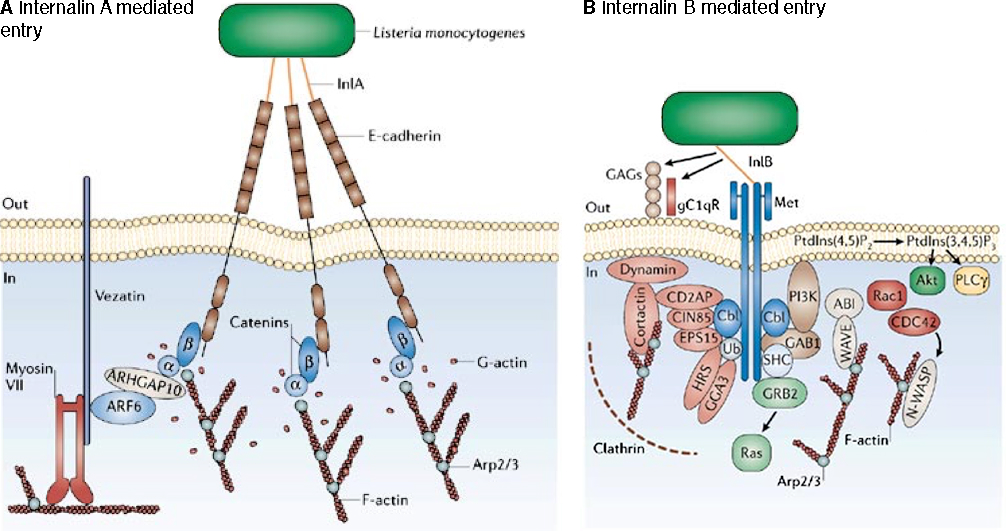
\includegraphics[width=0.8\textwidth]{listeria}
  \caption[Capsid structure and genome of rhinoviruses.]{Capsid proteins VP1 through VP4 form a pseudo $T=3$ icosahedral coat, roughly 30 nm in diameter around the RNA genome (A), which is monopartite, linear, 7.2 kp long and encodes 11 proteins (B). Figures adapted from \cite{Lebreton2015}.}
  \label{fig:listeria}
\end{figure}

\paragraph{Pathogenesis.}
The predominant entry path for \textit{L. Monocytogenes} into the human body is via the gastrointestinal tract, where Peyer's patches are targeted. The bacteria can induce cellular uptake (see section \ref{zipper-mechanism}), even by non-phagocytic host cells via expression of cell-surface associated interanlins. Upon cell entry, the phagosomal membrane is lysed, mediated by haemolysin secretion, and actin polymerization (see section \ref{subsec:actin-motility}) provides means of intracellular movement. Listerial haemolysin (listeriolysin) is acid activated with an optimum around pH 5.5, which is reached in late endosomes and membrane lysis is caused by the formation of large transmembrane pores. Growth and replication occur in the cytoplasm and adjacent cells can be entered by pushing against the plasma membrane and forming a pseudopod-like structure which in turn is taken up the neighbor. The resulting double-membrane vacuole can be escaped by cytolysis.

In an extracellular setting, haemolysins serve to rupture erythrocytes in order to generate free iron, a limiting growth factor. Furthermore the nonspecific immune system has to be evaded and haemolysins have also been shown to be cytotoxic towards leukocytes. Additionally, expression of bacterial superoxide dismutase mitigates the effect of free superoxide radicals which play an important role in killing phagocytized bacteria.

\paragraph{Epidemiology.}
Incidence of listeriosis has initially been increasing since its recognition as food-borne disease but effects of awareness and diagnostic methods are unclear. While typically long incubation periods do pose difficulties for clinical diagnosis, the number of susceptible individuals is on the rise and certain aspects modern processing and handling of foods may be beneficial for growth of \textit{L. Monocytogenes}. Disease rates of 2--15 cases per million population per year have been reported and listeriosis is among the leading case of lethal food-borne pathogen infections. Most recent data, however suggests, that incidence is decreasing again.

Due to its non-fastidious lifestyle, \textit{L. Monocytogenes} has been isolated from a wire array of ecological niches, including soil, sewage and water (both fresh water bodies and estuaries). High persistence (up to 4 years) in soil samples is problematic when contaminated manure is used as fertilizer and biofilm formation poses challenges for eradication from food processing plants. Additionally, the ability to grow in refrigerated foods and resistance towards heat treatment such as pasteurization warrant alertness and special preventive care. Many different foods have been implicated in listeriosis outbreaks, including vegetables (potatoes, radishes and celery), seafood (shrimp, crabmeat and smoked fish), diary products (soft cheese, pasteurized and unpasteurized milk) and meats (poultry, various types of sausages and pâté).

Despite high prevalence in food (studies have found 20--80\% of meat product samples and 1--10\% of diary product samples contaminated with \textit{L. Monocytogenes}), comparatively few successful infections occur. The bacteria are ingested frequently in small doses and stool sample examinations suggest that 10-70\% of investigated populations could be intestinal carriers. While the minimum infectious dose has not been settled definitively, approximations range from $10^6$ to $10^9$ bacteria.

\subsection{\textit{Salmonella} Typhimurium}
\textit{Salmonella} are non-sporulating, Gram-negative bacilli, belonging to the family Enterobacteriaceae. The motile bacteria are able to produce peritrichous flagella and diameters span 0.7 to 1.5 \textmu m while typical lengths range from 2 to 5 \textmu m. They are closely related to the genus \textit{Escherichia}, showing only 15\% chromosomal sequence disparity. Currently, two distinct species, \textit{S. bongori} and \textit{S. enterica}, within the genus \textit{Salmonella} are recognized, both of which are pathogenic towards a wide array of hosts. \textit{S. enterica} is further divided into 6 subspecies, the most relevant of which for human and domestic animal hosts being \textit{enterica}. A large number of serovars (more than 2500) for \textit{S. enterica} subsp. \textit{enterica} have been characterized and due to an originally mistaken classification as separate species, some serovars are designated with shortened names. \textit{S.} Typhimurium, therefore is shorthand for \textit{S. enterica} subsp. \textit{enterica}, serovar Typhimurium and to emphasize that Typhimurium is not a species description it is not italicized.

The first description of the genus \textit{Salmonella} dates back to an investigation into swine fever led by Salmon and Smith in 1885. The newly isolated bacterium was wrongly proposed as the etiological agent, as the disease later tuned out to be caused by a virus \citep{Fabrega2013}.

\paragraph{Diseases.}
Two distinct disease patterns are associated with \textit{Salmonella} spp. infections, typhoid fever and salmonellosis. While the former is exclusively caused by the serovars Typhi and Paratyphi, the latter is associated with several serovars, the most frequent being Enteritidis and Typhimurium, accounting for 65\% and 12\% of cases worldwide. The current and following sections will not discuss typhoid fever.

Salmonellosis is a diarrheal disease with a short incubation period of 6--24 h, followed by nausea, vomiting, loose or liquid bowel movements, abdominal cramps and fever. Clinical features are similar to those of dysentry and other gastroenteric disease and can include bloody and mucosal stool. In most cases, the infection is self-limiting and symptoms fade away within 4 to 7 days. The most common complication is bacteraemia, which presents in 5\% of cases and is more likely to develop in children, especially if malnourished, and immunocompromised individuals. Further manifestations of invasive infections include meningitis, osteomyelitis, cholangitis, pneumonia and endocarditis. While mortality in immonocompetent hosts in developed countries is as low as 0.1\%, it can increase to 77\% for \gls{hiv} positive patients in undeveloped countries.

\begin{figure}[t]
  \centering
  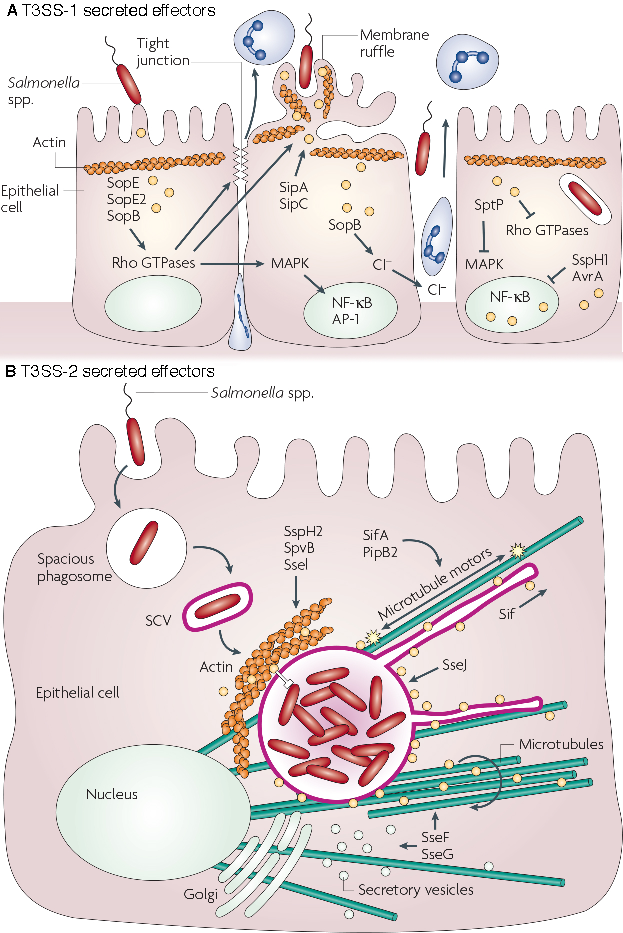
\includegraphics[width=0.7\textwidth]{salmonella}
  \caption[Capsid structure and genome of rhinoviruses.]{Capsid proteins VP1 through VP4 form a pseudo $T=3$ icosahedral coat, roughly 30 nm in diameter around the RNA genome (A), which is monopartite, linear, 7.2 kp long and encodes 11 proteins (B). Figures adapted from \cite{Haraga2008}.}
  \label{fig:salmonella}
\end{figure}

\paragraph{Pathogenesis.}
In order to reach the small intestine, ingested \textit{S.} Typhimurium first are exposed to the hostile environment of the stomach. A set of proteins, summarized as \gls{atr} helps mediate the acidic conditions and improves survival rates. The reamining bacteria subsequently reacht the small bowel and target its epithelial cells, with preference towards \gls{m-cells}. Flagellar motility enables penetration of intestinal mucus secretions and improves the chance of reaching the intestinal walls where adhesion can be established. Fimbriae are important attachment factors, capable of interaction with host-cell laminin and fibronectin and provide an initial platform for pathogen induced phagocytosis via trigger mechanism (see section \ref{trigger-mechanism}). 

\textit{S.} Typhimurium utilize two separate \gls{t3ss} systems for host-cell colonization, the first of which (\gls{t3ss}-1) mediates invasion. In addition to strengthening initial interactions attaching the pathogen to its target, the needle like structure serves as delivery mechanisms, capable of injecting effector proteins, including \gls{sop}E, \gls{sop}E2, \gls{sop}B (also known as SigD) and \gls{sip}A. \Gls{sop}E serves as \gls{gef} and activates \gls{rac-1} and \gls{cdc-42} via \acrshort{gdp}/\acrshort{gtp} exchange, which in turn initiate cytoskeletal rearrangements. \Gls{sop}E2 is a further \gls{gef}, highly homologous to \gls{sop}E and it is assumed to fill in for \gls{sop}E in \textit{Salmonella} strains missing the \gls{sop}E gene. \Gls{sop}B is a phosphatase, capable of hydrolyzing various substrates, including \gls{i13456p5}, which has been linked to intestinal fluid secretion causing diarrhea and \gls{pi45p2}, which is involved with membrane rigidity. Finally, the actin binding protein \gls{sip}A  stimulates stimulates actin polymerization and promotes membrane ruffling.

Upon engulfment, maturation of the phagosome and fusion with lysosomes have to be prevented. Unlike other pathogens that escape the digestive mechanisms of phagocytic vesicles by moving to the cytosol, \textit{Salmonella} replicate inside phagosome-derived \glspl{scv}. In this setting, the second translocation complex (\gls{t3ss}-2) is activated, and used to secrete effectors, including SsaB and SifA, capable of interacting with vesicular trafficking mechanisms and guiding the \gls{scv} away from its original degradation pathway. Furthermore \gls{t3ss}-2 translocated effectors induce actin polymerization events, which guide the \gls{scv} toward a perinuclear position. A last step in creating the intracellular niche needed for replication, is formation of \glspl{sif}, extending outwards from the \gls{scv}. \Gls{t3ss}-2 secretes effectors such as SifA, PipB2, SseF and SseG, which mediate the microtubule dependent processes by bundling and accumulating microtubules and regulating microtubule motor function.

\paragraph{Epidemiology.}
The global disease burden caused by nontyphoidal salmonellosis is estimated at 90 million cases per year and 150000 deaths. Incidence rates are highest in East and Southeast Asia (up to 4000 cases per 100000 population per year) and both developed and undeveloped countries are affected (incidence rates in Africa are estimated at 320 while estimates for Europe are around 690 cases per 100000 population per year). An estimated 80.3 million or 86\% of reported cases are food borne \citep{Majowicz2010}.

In order to control \textit{Salmonella} outbreaks, preventive measures in food production and processing is of major importance. This starts with disease containment in domestic animals, such as vaccination of chickens, enforcing  hygiene standards in manufacturing and distribution facilities and ends with proper preparation, exploiting heat sensitivity of the organisms. As the main route of transmission is fecal--oral, good sanitary infrastructure, treatment of sewage and water processing are crucial prerequisites in combating outbreaks of salmonellosis.
% minimum infectious dose + biofilm formation leading to asymptomatic presistence

\subsection{\textit{Shigella Flexneri}}
Shigellae are small, non-sporeforming, Gram-negative bacilli and belong to the family \textit{Enterobacteriaceae}, along with \textit{Escherichia}, \textit{Salmonella} and \textit{Yersinia}. While flagellar genes are present and their expression is observed under certain conditions, the bacteria are usually described as non-motile and unflagellated. The facultative intracellular parasite shows strong specificity towards human hosts where it typically infects the lower gastrointestinal tract.

\textit{Shigella dysenteriae} was identified as the etiological agent of dysentery by Shiga in 1897 during an epidemic in Japan with 91000 reported cases and a \textgreater 20\% mortality rate. \textit{S. Flexneri} was first described by Flexner in 1900, while investigating diseases endemic to the Philippines. Recent genetic studies suggest, that \textit{Shigella} spp. belong to the species \textit{Escherichia coli}, rather than forming a distinct genus, as only marginal sequence divergence (1.5\%) between \textit{E. coli} and \textit{S. Flexneri} was found \citep{Schroeder2008}.

\paragraph{Diseases.}
Bacillary dysentery is an acute infection of the intestine. Mild cases of the disease are self-limiting and afebrile with diarrhea and possibly vomiting as the only symptoms. In as little as 24 hours after onset, bowel movements usually begin to normalize and the condition is resolved within a few days. More severe cases are accompanied by strong abdominal cramps, fever and watery diarrhea containing blood and mucus, indicative of injury to the intestinal epithelium. While still usually self limiting in healthy individuals, recovery takes 10--14 days and relapses are possible. In immunocompromised patients, young children, especially if malnourished, and elderly individuals, life threatening complications including bacteraemia, renal failure, intestinal perforation and toxic megacolon are more frequent. Involvement of the central nervous system and respiratory tract is rare.

Administration of antibiotics is not recommended in mild to moderate cases as the disease can usually be overcome by the immune system and \gls{amr} in Shigellae is becoming an increasing concern. Oral rehydration therapy is the most effective treatment, helping the body replenish liquids and salts lost due to diarrhea. For severe infections, the use of antibiotics can become necessary and testing for resistance patterns, if possible, is advised.

\begin{figure}
  \centering
  \includegraphics[width=0.95\textwidth]{shigella}
  \caption[Capsid structure and genome of rhinoviruses.]{Capsid proteins VP1 through VP4 form a pseudo $T=3$ icosahedral coat, roughly 30 nm in diameter around the RNA genome (A), which is monopartite, linear, 7.2 kp long and encodes 11 proteins (B). Figures adapted from \cite{Croxen2010}.}
  \label{fig:shigella}
\end{figure}

\paragraph{Pathogenesis.}
Main targets of \textit{S. Flexneri} are mucosa of the distal ileum and colon where they enter epithelial cells from the basolateral side. For initial crossing over from the apical side, action of \gls{m-cells} at Peyer's patches is exploited. These specialized enterocytes constantly sample antigens from the gut lumen and pass them to intraepithelially located dendritic cells and lymphocytes. Upon uptake by basolaterally located macrophages, \textit{S. Flexneri} survive digestive action of the phagosomal vacuole by disrupting the surrounding membrane and initiating host-cell apoptosis, mediated by the bacterial effector protein \gls{ipa}B, capable of acting on a caspase 1 regulated apoptotic pathway. The bacteria are subsequently released into the sub-mucosa, where they induce phagocytosis by normal epithelial cells via trigger mechanism (see section \ref{trigger-mechanism}).

Initial contact between pathogen and target hos cell is mediated by cellular \textalpha\textsubscript{5}\textbeta\textsubscript{1} integrins and binding of \gls{ipa}B to CD44 receptors may initiate first actin rearrangements, preparing the cell for uptake. Subsequent injection of at least 6 effector proteins into the epithelial cytosol through the \gls{t3ss} triggers engulfment of the bacterium in an actin dependent process, involving the small GTPases \gls{rac-1} and \gls{cdc-42}, which recruit the actin nucleation complex \gls{arp-2-3}. \Gls{ipa}C, a component of the translocation complex, is involved in stimulating \gls{rac-1} and \gls{cdc-42} GTPase activity through an unknown mechanism and the secreted effector proteins IpgB1, IpgB2, IpgD and \gls{ipa}A facilitate actin polymerization. IpgD, an inositol phosphate phosphatase, catalyzes the hydrolysis of \acrshort{pi45p2} to \acrshort{pi5p} which promotes disassociation of cytoskeleton and membrane, increasing actin availability and making the plasma membrane more susceptibility to manipulation. The mechanism of action of IpgB2 remains to be resolved, while IpgB1 is assumed to mimic activated \glsrev{rho-g}, a small GTPase, located upstream in the signaling pathway of \gls{rac-1}. Finally, binding of \gls{ipa}A to vinculin induces depolymerization of actin, which is assumed to be important for closing of the phagocytic cup.

The resulting phagocytic vacuole has to be escaped before maturation progresses, which is accomplished in a non-acid dependent fashion, by the translocator proteins \gls{ipa}B, \gls{ipa}C and \gls{ipa}D via membrane lysis. With release into the epithelial cytosol, the replicatory niche of \textit{S. Flexneri} is reached. Actin mediated intracellular motility enables intercellular dissemination (see section \ref{subsec:actin-motility}) and targeting of epithelial tight junctions initiates break-down of the epithelial barrier, providing more pathogens with access to the basolateral side of the gut lining.

Host-cell actin utilization, is driven by activity of two bacterial proteins. VirA is secreted at the forward facing end of the rod shaped bacilli, which promotes degradation of tubulin structures and therefore clearing a path through the dense network of microtubules and surface bound \glsrev{ics}A facilitates actin polymerization at the opposite end. Both \gls{arp-2-3} and \gls{n-wasp} are involved in actin nucleation, the directed nature of which provides the driving force for locomotion.

\paragraph{Epidemiology.}
Estimates by the \gls{who} peg the disease burden caused by \textit{Shigella} spp. at 80 million annual cases worldwide, leading to 700000 deaths. Developing countries are disproportionately affected, representing 99\% of all cases, as are children less than 5 years old, accounting for 70\% of cases and 60\% of deaths. In developed countries, incidence rates of 1--2 per 100000 population are typical and Shigellae are common causes of Traveler's diarrhea.

The predominant route of transmission is fecal--oral, highlighting the importance of sanitary precautions for infection control. Proper treatment of fecal matter is important for preventing contamination of drinking water and inhibiting spreading by disease vectors such as house flies. During acute phases, diseased individuals excrete pathogens in large numbers and as few as 100--200 organisms are sufficient of causing a new infection.

\section{Select Viral Pathogens}

In addition to the previous 5 bacterial pathogens, 3 viruses were selected for study within the InfectX RTD project by SystemsX. This section shortly describes each pathogen in terms of physical features, pathogenesis, epidemiology and diseases caused in humans. For each section, a chapter of \cite{Craighead2000} serves as basis.

\subsection{Adenoviruses}
The family \textit{Adenoviridae} encompasses 5 genera of non-enveloped, medium sized (90 nm diameter) viruses, capable of infecting a broad range of vertebrate hosts. The capsid is of $T=25$ icosahedral symmetry, composed of 720 hexons arranged as 240 trimers which form the triangular facets and 12 penton capsomeres located at the vertices. A homotrimeric fiber glycoprotein protrudes from each vertex, attached to the penton base via interactions of its N-terminal domains and ending in a globular, C-terminal knob. The genome is present as double stranded DNA (Baltimore group I), is non-segmented, linear, 35--35 kb long and encodes 40 proteins.

Adenoviruses were first isolated from human adenoid tissue cultures by Rowe in 1953 and their study led to the discovery of alternative splicing in 1977, a commonly encountered phenomenon among eukaryotes. Currently, 57 serovars are recognized as pathogenic towards humans, all belong to the genus \textit{Mastadenovirus} and are classified into 6 species, labeled A through G. The following sections are mostly concerned with \textit{Human adenovirus C} \citep{Lenaerts2008}.

\paragraph{Diseases.}
In immunocompetent individuals, adenoviruses seldom cause more than transient disease with many infections even occurring subclinically and fatal outcome being very uncommon. Symptomatic cases usually manifest as respiratory tract infections or conjunctivitis and less frequently as hemorrhagic cystitis, nephritis or gastroenteritis. Infections of the oropharynx can spread to the lower respiratory tract, causing bronchitis, bronchiolitis or pneumonia, which can become chronic, leading to desquamated epithelial tissue and long-term damage to the respiratory mucosa. Heart failure and central nervous system involvement can occur in severe cases. Ocular infections range from mild, short-term follicular conjunctivitis to highly contagious keratoconjunctivitis with possible long-term damage to the cornea. \textit{Human adenovirus C} serotypes are mostly associated with respiratory diseases but have also been implicated in eye infections.

Invasive forms of disease are mostly limited to immunocompromised individuals, including transplant recipients, \gls{hiv} infected, hereditary immunodeficient and cancer patients subject to chemotherapy. In addition to the lungs, a wide variety of organs has been reported to be affected, such as partoid glands, liver, gall bladder, colon, brain and kidney and pathological changes range from perivascular cuffing to parenchymal necrosis.

\begin{figure}
  \centering
  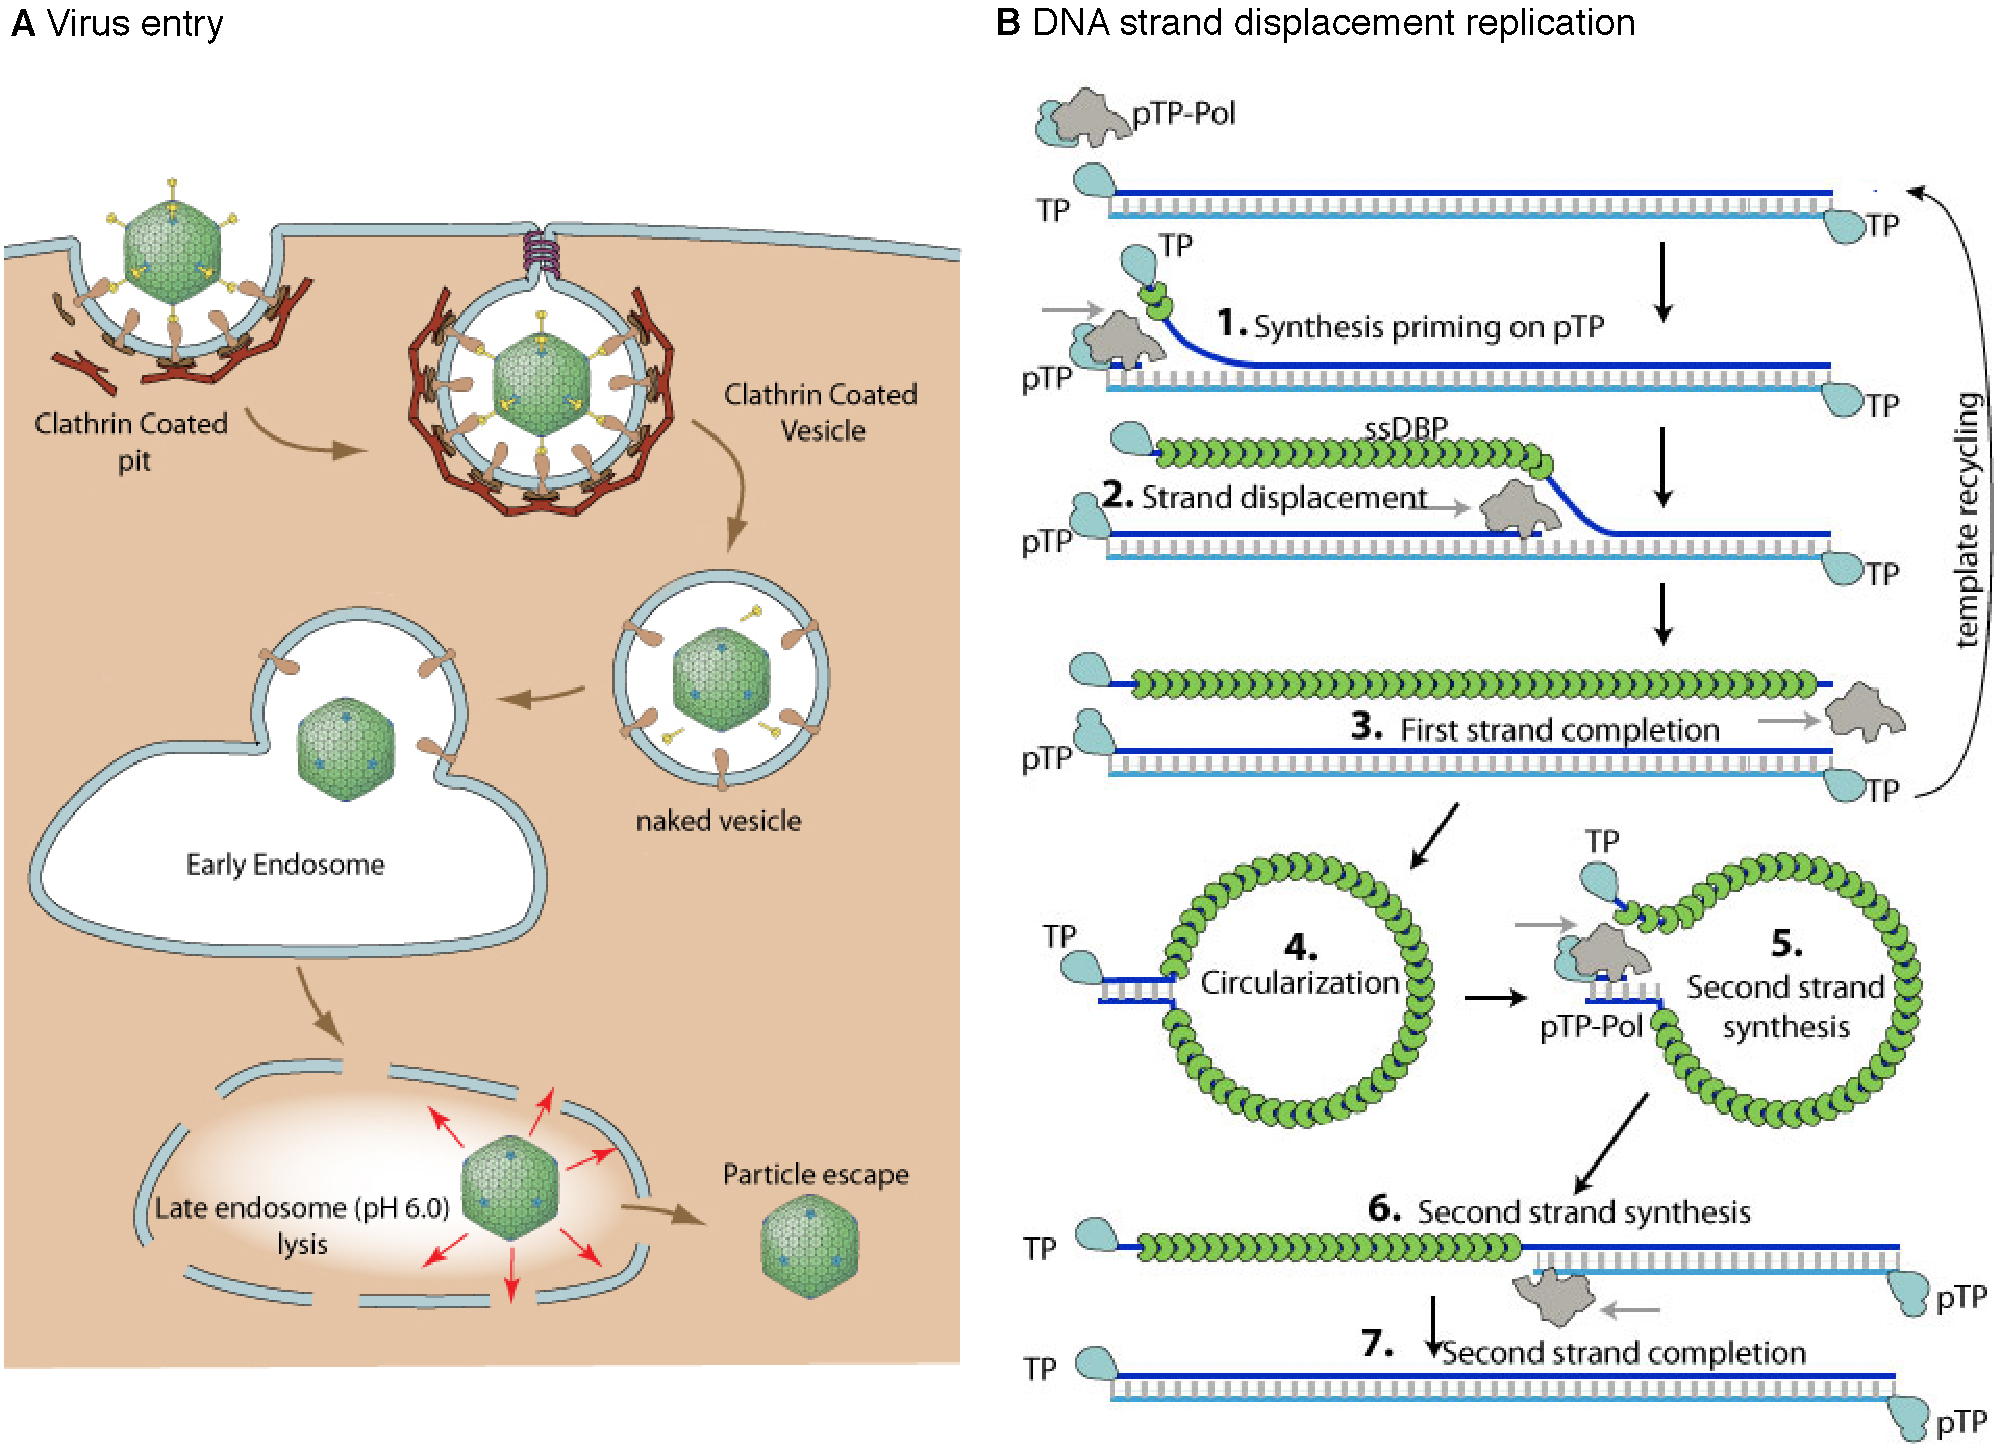
\includegraphics[width=0.95\textwidth]{adenovirus}
  \caption[Capsid structure and genome of rhinoviruses.]{Capsid proteins VP1 through VP4 form a pseudo $T=3$ icosahedral coat, roughly 30 nm in diameter around the RNA genome (A), which is monopartite, linear, 7.2 kp long and encodes 11 proteins (B). Figures adapted from \cite{Hulo2011}.}
  \label{fig:adenovirus}
\end{figure}

\paragraph{Pathogenesis.}
Initial attachment of virions is mediated by interactions between the globular knobs of viral fiber proteins and target cell \glsrevpl{car}. In \textit{Human adenovirus C} infections, cellular heparan sulfate proteoglycans serve as additional attachment factors, reinforcing adhesion. Subsequent binding of penton bases to \textalpha,\textbeta-integrin receptors induces clathrin-mediated endocytosis and leads to loss of viral fiber proteins.

The adenoviral replication cycle is divided into early, intermediate and late stages, with each seeing expression of a typical set of genes. Upon engulfment by the host cell and triggered by endosomal acidification, hexon bound protein VI disassociates from the capsid structure and induces lysis of the endosomal membrane. The remainder of the now cytosolic virion is shuttled to the nucleus by microtubular transport where viral protein IX recruits kinesin thereby procuring capsid disruption. Nuclear penetration is mediated by core protein VII and occurs at \glspl{npc}, leading to transcription of early viral genes by host RNA polymerase II. The resulting proteins manipulate various cellular processes, such as evasion of host immune response (E3), cell cycle (E1A), apoptosis (E1B and E4) and \gls{mrna} transport (E4), while also promoting viral DNA replication (E2). A virally encoded DNA polymerase replicates the genome by DNA strand displacement in a unique protein primed fashion involving \gls{ptp} acting as primer and \gls{dbp}, as well as several host proteins. With onset of replication, translation of late genes by host RNA polymerase II is initiated, leading to the production of structural proteins and proteins required for virion assembly. Encapsidation occurs in the nucleus and progeny virions are released by lysis of the host cell.

\paragraph{Epidemiology.}
Adenoviruses are endemic and ubiquitous, causing an estimated 2--5\%of all respiratory infections. Distribution is worldwide and incidence higher in the first half of the year. Children are frequently infected as serological studies show that by the age of 5 years some 50\% present antibodies towards the most common species, including \textit{Human adenovirus C}. On the order of 1 in every $10^7$ lymphoid cells in the oropharynx harbor fully assembled latent sate virions, making most humans latent carriers. Transmission can both occur via respiratory droplet or fecal-oral routes and virions are very stable towards chemical and physical agents, surviving for long periods outside their host.

Adenovirus outbreaks are a common cause of pneumonia in militaries, leading to the development of live, oral vaccines in the 1960's by the U.S. Army. The only supplier however ceased production and as of 1999, vaccinations could no longer be administered, resulting in reemerging incidence. In the first 5 years after loss of the vaccine, 110000 cases of febrile respiratory illness were reported, of which an estimated 90\% are considered preventable. By October 2011, new vaccine again was available and and has been administered to new recruits since.

\subsection{Rhinoviruses}
Investigations into the etiological agent of the common cold within the British Common Cold Research Unit led to the discovery of rhinoviruses in 1953. Initially classified as a separate genus of the family \textit{Picornaviridae}, recent genomic evidence led to a revised taxonomy, recognizing three species of rhinoviruses (A through C) as members of the genus \textit{Enterovirus}. Over 100 distinct serotypes have been isolated from humans, 74 belong to species A, 25 to B and the newly identified species C, currently under active study, may encompass an additional 55 types.

Rhinovirus virions are small (30 nm in diameter), non-enveloped, with a pseudo $T=3$ icosahedral capsid, consisting of 4 different polypeptides (VP1, VP2, VP3 and VP4) surrounding the RNA genome. There are 60 copies of each structural protein and VP1-3 face towards the outside and are responsible for antigenic diversity, while VP4 faces inwards and anchors the RNA core to the capsid. A canyon formed by VP1 and VP3 serves as receptor binding site. The viral genome consists of monopartite, linear, single stranded, positive sense RNA, roughly 7.2 kb in length and encodes a single polyprotein, which cleaved by viral proteases yields 11 proteins. Instead of a methylated 5' cap, the RNA genome is terminated by a viral protein (VPg) at its 5' end \citep{Jacobs2013}.

\paragraph{Diseases.}
Over half and up to two thirds of all cold-like illnesses are thought to be caused by rhinoviruses. In addition, asymptomatic infections, especially in children are very common with rates among children under 4 years ranging from 12 to 32\%. These surprisingly high numbers may to some extent result from virus persistence in hosts that have recovered in addition to disease that has not broken out. In adults, rates of asymptomatic carriage are significantly lower, reported at 0--2\%.

In immunocompetent individuals, symptomatic disease typically manifests as upper respiratory infection with clinical syndromes associated with common cold, including rhinorrhea, nasal congestion, sore throat, headache and possibly fever and general malaise. Disease is self-limited, incubation periods are between 12 and 72 h and within 7 to 14 days, symptoms wear off. A common complication is acute otitis media, which has been reported to happen in up to 30\% of cases in early childhood. In 41--45\% of investigated middle ear infections, rhinoviruses were detected. Further cavities that are frequently infected are the paranasal sinuses. Nose blowing has been suggested as mechanism for spreading the virus and causing rhinosinusitis.

Initially thought to primarily cause benign upper respiratory infections,  recent data clearly implicates rhinoviruses in more severe lower respiratory infections. Croup, bronchiolitis and \gls{cap} have been associated with rhinovirus infections and studies have shown that in 12, 14 and 18--26\% of respective cases, rhinoviruses were present. Furthermore, a study of children admitted to \glspl{icu} with lower respiratory tract infections detected no other pathogens in 49\% of the patients. Immunocompromised individuals are predisposed to contracting more serious forms of disease, with morbidity and mortality comparable to that of pandemic H1N1 influenza.

While not typically associated with cytopathogenic effects on epithelia of the upper respiratory tract, cell damage to lung tissue, especially among children, has been documented. Thus, rhinoviruses are linked to exacerbations of chronic pulmonary diseases such as asthma, chronic obstructive pulmonary disease and cystic fibrosis.

\begin{figure}
  \centering
  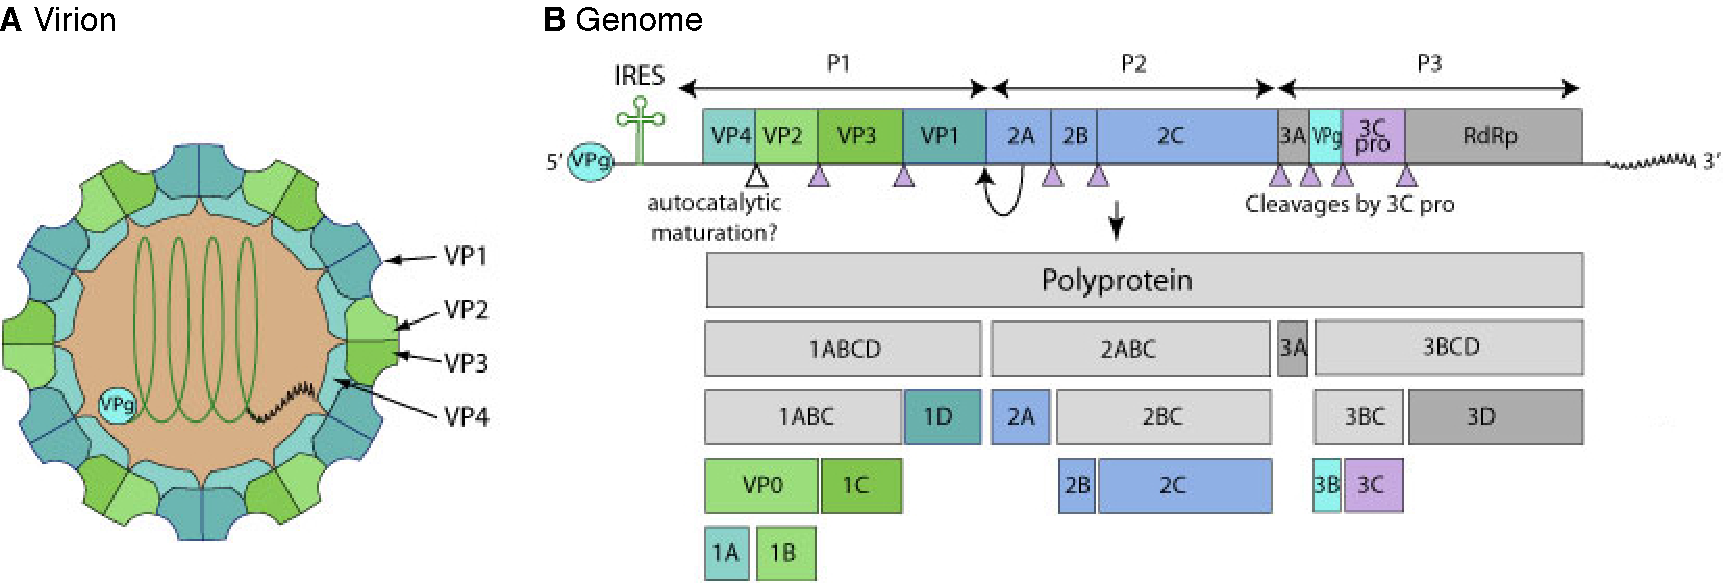
\includegraphics[width=0.95\textwidth]{rhinovirus}
  \caption[Capsid structure and genome of rhinoviruses.]{Capsid proteins VP1 through VP4 form a pseudo $T=3$ icosahedral coat, roughly 30 nm in diameter around the RNA genome (A), which is monopartite, linear, 7.2 kp long and encodes 11 proteins (B). Figures adapted from \cite{Hulo2011}.}
  \label{fig:rhinovirus}
\end{figure}

\paragraph{Pathogenesis.}
Members of rhinovirus species A and B are divided into two group according to their host cell receptors. Members of the major group form interactions with \gls{icam-1} while minor group types (including serotype 1a) associate with \glspl{vldlr}. Attachment of species C have very recently been identified as induced by \gls{cdhr3}. Upon receptor mediated endocytosis, pH dependent conformational changes in capsid structure exposes VP4 which has pore-forming properties and facilitates release of viral genomic material into the cytosol.

Host cell ribosomes readily translate the released positive-sense RNA into polyprotein, which is cleaved in \textit{cis} by 2A and 3Cpro, yielding preproteins P1, P2 and P3 (see figure \ref{fig:rhinovirus}. P1 is digested into structural capsid proteins while P2 and P3 are further processed to produce the replication machinery. Viral RNA-dependent RNA polymerase synthesizes a complementary, negative-sense RNA strand, primed by VPg, which in turn serves as template for many copies of the viral genome. These can be both translated into more protein and in a later stage of replication also be packaged into progeny virions. Final cell export is mediated by host-cell membrane lysis.

\paragraph{Epidemiology.}
Despite most infections with rhinoviruses only resulting in mild disease, economic impact both due to health care costs and loss of productivity is considerable. This is primarily owed to the overwhelming prevalence of these pathogens. Respiratory illnesses attributed to rhinoviral infections occur throughout the world and all year round with peak incidences in early fall and spring. Vaccination efforts so far have been futile, mainly because of the large number of serotypes and lack of individual epidemiological data.

Due to acid-sensitivity, fecal-oral infection is unlikely most person-to-person transmission occurs through aerosols and contact spread either direct of via fomites. Extra-host survival times of hours to days have been reported for indoor environments and up to 2 h on undisturbed skin.

\subsection{Vaccinia}
\textit{Vaccinia virus} is a species within the genus \textit{Orthopoxvirus}, alongside the exceptionally virulent \textit{Variola virus}, the etiological agent of smallpox. Immunological similarities between the two species allows for cross-protection, which coupled with the large discrepancy in pathogenicity presents a fortunate opportunity for artificially inducing acquired immunity. This was recognized by Jenner in 1798, while investigating the zoonosis of \textit{Cowpox virus} and subsequent susceptibility towards contraction of smallpox. The origins of vaccinia are unknown. It has been speculated to have derived from cowpox or smallpox, to be a hybrid of both and of being the prototype orthopoxvirus, as well as descending from an extinct ancestor.

The virions are large and brick shaped, measuring 200 by 250 by 340 nm and exist as both \gls{mv} and \gls{ev}. Structurally they are unusually complex. The linear, double-stranded DNA genome, roughly 200 kb long, is encased in an S-shaped, tube-like nucleocapsid with an outside diameter of 50 nm, a cavity of 10 nm and an overall length of 250 nm. Additionally, 47 viral proteins, of which 16 are involved in early \gls{mrna} synthesis and 28 have no known enzymatic function, are packed into a core structure. The core wall consists of two layers, the palisade (outer) layer which is 17 nm thick and an inner smooth layer, measuring 8 nm across. Centered on the top and bottom faces, two proteinaceous lateral bodies separate core from the surface membrane, forming the virion core into a biconcave disc with dumbbell shaped vertical cross sections. The lipidic surface membrane also consist of two layers, the outermost measuring 9 nm and the innermost domain is 5 nm thick. \Gls{ev} virions are additionally wrapped in a membrane derived from Golgi cisternae \citep{Marennikova2005,Condit2006}.

\paragraph{Diseases.}
While infection with variola causes severe disease manifesting in skin lesions covering the whole body, accompanied by 20--40\% mortality rates, the closely related \textit{Vaccinia virus} is far less invasive. Virulence of the latter pathogen is so low that it has been routinely used as live vaccine against the former. Owing to the massive effort put into the worldwide fight against smallpox led by the \gls{who} in the late 1960's and throughout the 1970's, the disease was found to be eliminated by 1980. At the center of the smallpox eradication program was the administration of freeze-dried, calf lymph derived vaccinia with a bifurcated needle, by multiple pricking of the skin. Towards the end of the initiative, 200 million vaccinations were performed annually.

The predominant reaction to vaccinia inoculation is localized, self-limited disease. After an incubation period of of 3--4 days, a papule with a sunken center develops at the site of infection, accompanied by erythema and swelling. Over the following days the papule increases in size and liquid begins to accumulate within. Fever may develop around days 7--10, possibly followed by malaise, headache and anorexia. Local lymphadenopathy is frequently encountered and days 8--10 typically mark the beginning of involution of the papule, which subsequently drys out and forms a scab.

Of great concern for routine vaccination procedures are complications which inevitably occur in a small numbers. Atypical side effects develop in roughly 1 per mill of cases and potentially life threatening reactions usually manifest as neurological (477.4 cases and 47.0 fatalities per 1 million) or cutaneous disease (278.4 cases and 0.2 fatalities per 1 million). Predisposing conditions for central nervous system involvement are not known and despite decades of inquiry into this pathology, it remains poorly understood. Symptoms range from febrile seizures to severe encephalitis, but so far no  neuropathological characteristics have been identified. Complications affecting the skin and mucous membranes are classified as progressive vaccinia, eczema vaccinatum and generalized vaccinia and disease severity decreases in this order. Predisposing conditions for progressive and generalized vaccinia are immunodeficiencies while a history of eczema is a risk factor for eczema vaccinatum.

\begin{figure}[t]
  \centering
  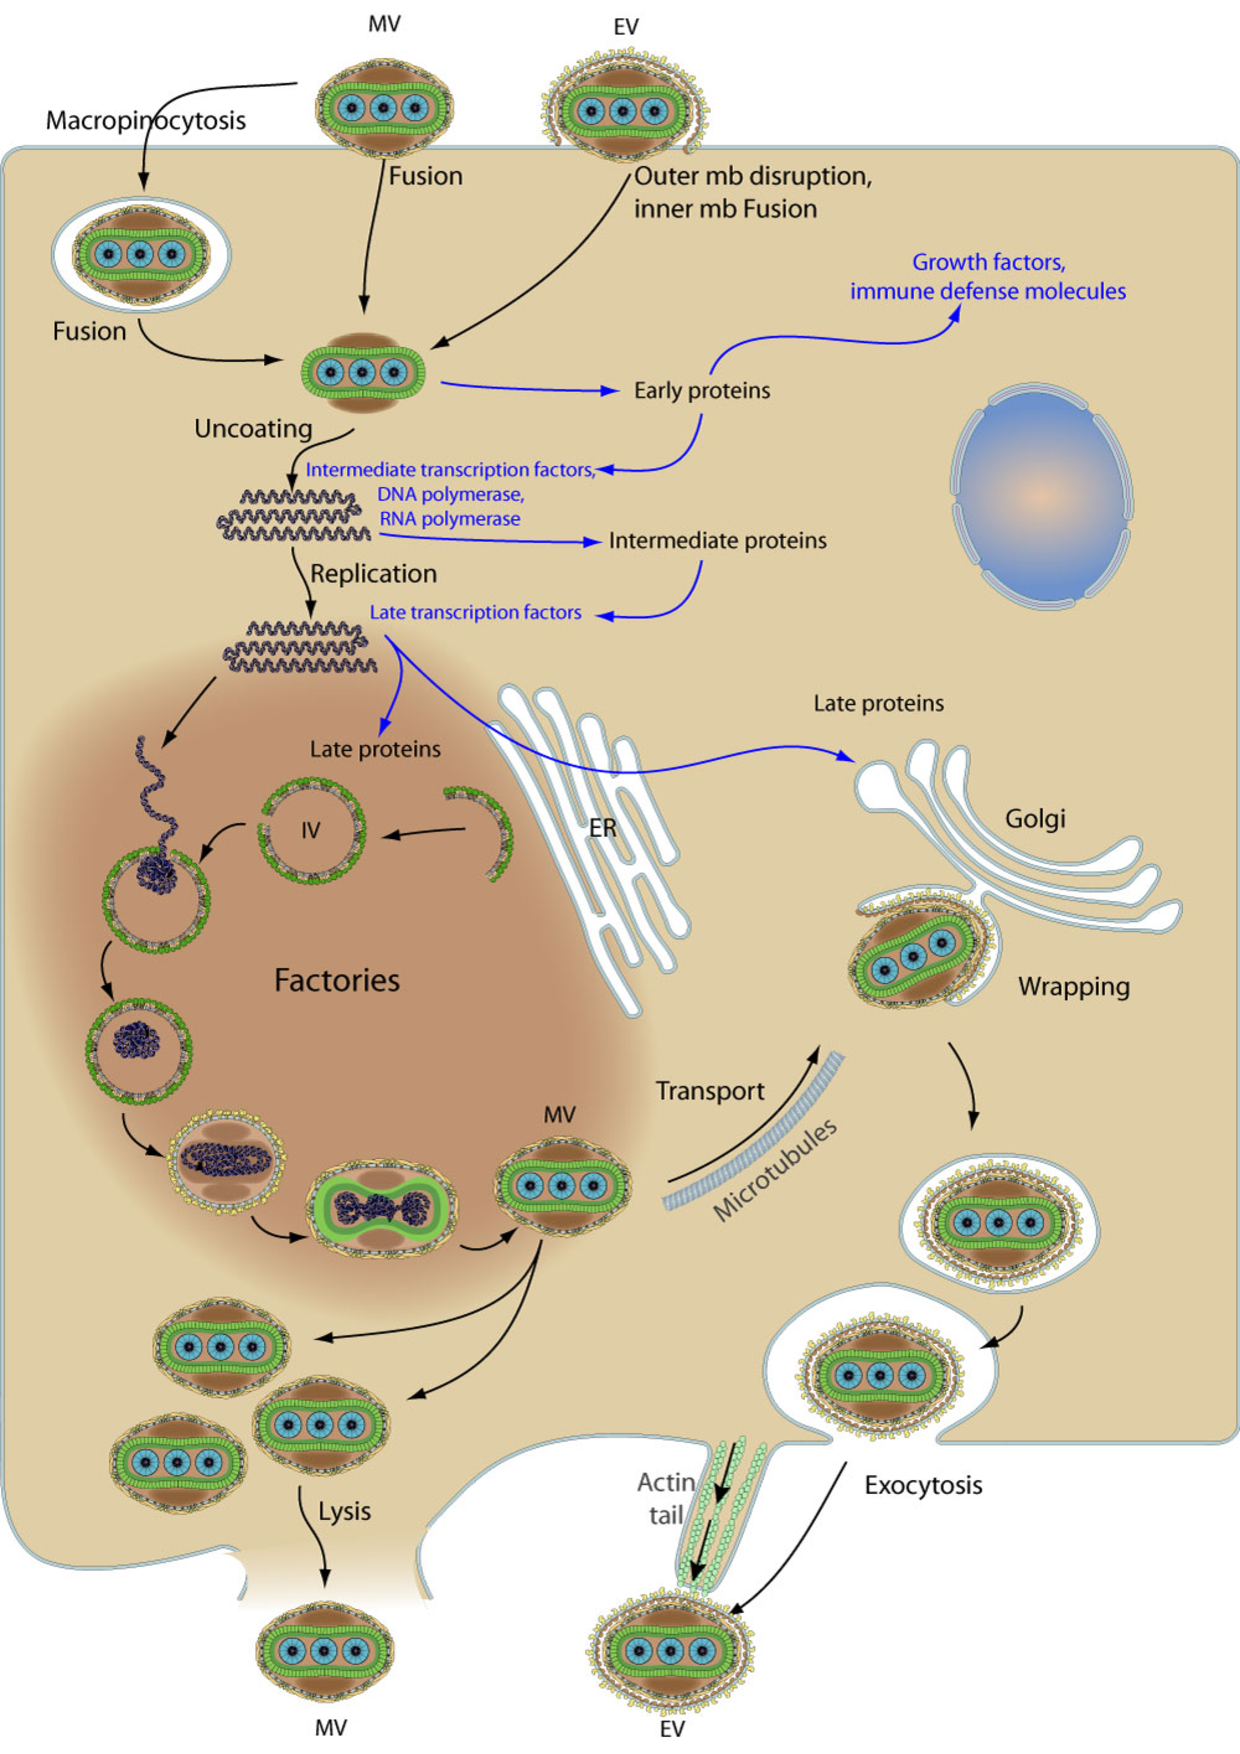
\includegraphics[width=0.75\textwidth]{vaccinia}
  \caption[Replication cycle of \textit{Vaccinia viruses} for both intracellular mature and extracellular enveloped virions.]{Capsid proteins VP1 through VP4 form a pseudo $T=3$ icosahedral coat, roughly 30 nm in diameter around the RNA genome (A), which is monopartite, linear, 7.2 kp long and encodes 11 proteins \citep{Hulo2011}.}
  \label{fig:vaccinia}
\end{figure}

\paragraph{Pathogenesis.}
Initial attachement is mediated by interaction between viral proteins and cellular heparan sulfate chains. For cell entry, various strategies have been reported, depending on the strain under investigation. WR strains induce macropinocytosis and proteins A25/A26 act as fusion suppressors that only lift their embargo under acidic conditions encountered in a maturing endosome, while other strains, such as Copenhagen, present no A25/A26 on their outer membrane and fuse directly with the target plasma membrane. Due to the additional membrane of \glspl{ev}, a differing entry mechanism needs to be emplyed. In a currently not well understood fashion, the outer membrane is lost by non-fusogenic disruption, followed by fusion of the inner virion membrane. All pathways lead to cytosolic localization of virions devoid of their envelope.

Members of the \textit{Poxviridae} family are special among Baltimore group I viruses in that their genome encodes all necessary replicatory proteins, allowing for cytosolic localization. Replication is temporally tightly regulated and consist of distinct phases of early, intermediate and late gene expression. Each class of genes encodes factors capable of initiating the succeeding stage, providing transcription level regulation. Uncoating of the core structure releases early proteins, including RNA polymerases and enzymes for \gls{mrna} processing which start transcribing early genes. At least 50 different products, such as DNA replicatory enzymes, additional RNA polymerase, \gls{mrna} processing machinery, host defense molecules and intermediate gene transcription factors, have been identified and account for 25\% of the viral coding capacity. Early gene transcripts are detectable 20 minutes after cell entry and reach their productive peak within 100 minutes of infection.

Expression of intermediate genes is initiated by accumulation of intermediate  transcription factors and the onset of DNA replication. Only 7 products of this phase are known, which functionally are mostly concerned with host defense, DNA/RNA metabolism and commencement of the final phase. Beginning 100 minutes after infection, intermediate gene transcription reaches its peak at 120 minutes and is thereafter superseded by late gene transcription, beginning 140 minutes after cell entry. Products of the final phase comprise a large number of genes (up to 75\% of the vaccinia genome) and include enzymes needed for initiating replication (RNA polymerase and modification proteins), early transcription factors and structural proteins, as well as virion assembly machinery.

DNA replication not only serves for progeny virions, but also to increase the concentration of templates used for gene expression. Both DNA synthesis and virion assembly occur within factories, readily visualized by electron microscopy as electron dense cytoplasmic inclusion bodies. Owing to the complex virion structure DNA packaging and virion assembly is an involved procedure with is incompletely understood.

\paragraph{Epidemiology.}
It is unknown if a natural reservoir of vaccinia exists It has been speculated that the virus is maintained only within research laboratories and vaccination production facilities, while others have implicated some rodent species as possible reservoir hosts. Small scale zoonotic outbreaks of vaccinia have been documented in Brazil and it was initially suspected that these were linked to vaccine that had escaped into the environment. Recent phylogenetic studies however were able to rule out this explanation but were unable to shed further light into underlying epidemiological mechanisms.

While transmission from vaccinees to unvaccinated individuals is rare, direct contact transmission is possible and such occurrences have been documented. Special care has to be taken to avoid direct contact between recently vaccinated and individuals predisposed towards developing complications.

\section{RNA Interference}
First described only two decades ago, regulation of gene expression by short strands of RNA has become an indispensable tool to both experimental biology and bioinformatics. Recognizing the importance of applications made possible by this discovery, the 2006 Nobel prize in Physiology or Medicine was awarded to Fire and Mello who studied RNA interference in the nematode worm \textit{Caenorhabditis elegans} and published their findings in 1998. Building on studies by Guo and Kemphues, who showed that sense RNA, as well as antisense RNA was capable of suppressing gene expression, Fire, Mello and coworkers found that double stranded RNA was at least ten-fold more effective as silencing agent than individual single stranded fragments. Further investigations showed that several gene regulatory processes, previously thought to be unrelated, were in fact manifestations of RNA interference and that the underlying mechanism was conserved in many if not most eukaryotic organisms \citep{Hannon2002}.

The RNAi pathway can take as input two separate types of RNA molecules, \gls{mirna} and \gls{sirna}, of differing origins. While \glspl{mirna} are endogenous and purposively employed in post-transcriptional regulation of gene expression, \glspl{sirna} are exogenous synthetic or viral inducers of gene suppression, in which case, RNA interference can be viewed as an immune response to foreign genetic material. Parsimony-based phylogenetic analysis of involved genes suggests that the key components to an RNAi system were already present in the last common ancestor of eukaryotes and were subsequently lost or extensivley simplified in some protists. The original function of RNAi is hypothesized to be that of a defense mechanism against genomic parasites as indicated by the extent of its conservation, whereas \gls{mirna}-directed silencing most probably was introduced at a later point in evolution \citep{Cerutti2006}.

\subsection{Molecular Mechanism}
RNA interference refers to three separate mechanisms for regulation of gene expression by small RNAs, as visualized by figure \ref{fig:rnai}. While \glspl{sirna} are involved both in transcriptional and post-transcriptional gene silencing, the \gls{mirna} pathway is focused on translational repression. The severity of action on the targeted genes once again highlights the differing purposes of the \gls{sirna} and \gls{mirna} pathways, one tasked with inhibitory and the other with regulatory measures \citep{Wilson2013,Kim2007,Carthew2009}.

\begin{figure}[t]
  \centering
  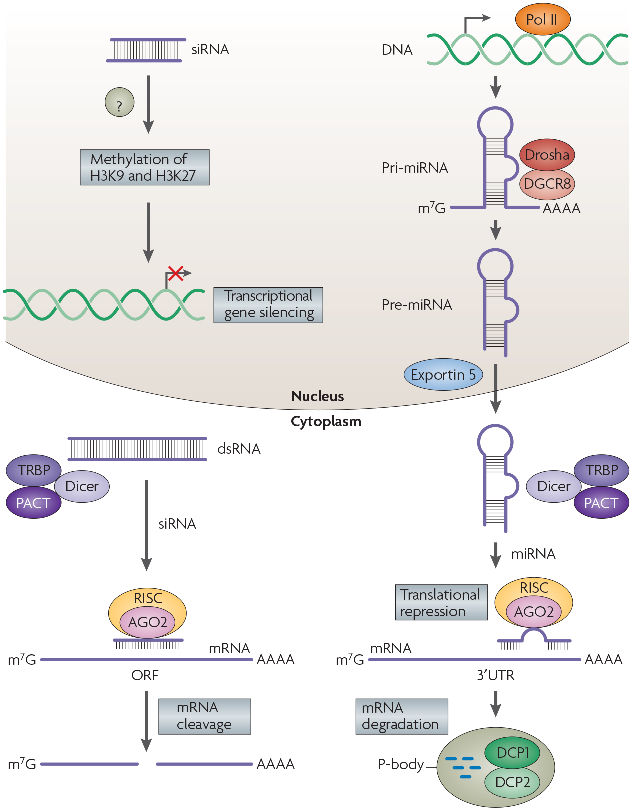
\includegraphics[width=0.7\textwidth]{rnai}
  \caption[The three major pathways of RNA interference.]{RNA interference comprises of three distinct mechanisms that yield control over gene expression. Exogenous double-stranded RNA are processed into \gls{sirna} fragments that both act inside the nucleus as transcriptional silencing agents and in the cytoplasm, post-transcriptionally cleaving \gls{mrna} strands. Endogenous \gls{mirna} is synthesized by RNA polymerase, originates from the nucleus in processed form and mediates milder translational repression \citep{Kim2007}.}
  \label{fig:rnai}
\end{figure}

\paragraph{Translational repression by \gls{mirna}.}
The biogenesis of \gls{mirna} occurs in the nucleus and is initiated by RNA polymerase II transcription of long (\textgreater 1000 nt) \gls{pri-mirna} segments, characterized by double-stranded hairpin loops with single-stranded 5'- and 3'-terminal overhangs which are polyadenylated and capped. Subsequent processing by the microprocessor complex consisting of the RNase III family enzyme Drosha and \glsrev{dgcr8} yields \tilde 60--70 nt stem-loop structured \gls{pre-mirna} fragments. \gls{dgcr8} recognizes \glspl{pri-mirna} by the junction of stem and single-stranded overhang and helps positioning the substrate for endonucleolytic cleavage by Drosha at a site \tilde 11 nt from the junction. Nuclear export is mediated by the transport facilitator exportin-5 and is Ran-GTP dependent.

In the cytoplasm, \glspl{pri-mirna} are targeted by Dicer and the associated dsRNA binding proteins \glsrev{trbp} and \glsrev{pact} for further processing into 21--25 nt dsRNA strands with 2 nt overhangs at the 3' termini and phosphate groups at each of the recessed 5' ends. The mature \glspl{mirna} are loaded onto \gls{ago} by Dicer, which leads to the formation of \gls{risc}. Concomitantly with \gls{risc}-loading, one of the two RNA stands is selected as guide strand whereas its complement (the passenger strand) is ejected and degraded. Thermodynamic asymmetry between the two strands is exploited in this step and the strand with the less stable 5' end is preferred. As opposed to strand separation in \glspl{sirna}, the passenger strand is not cleaved but rather unwound by helicase activity, facilitated by imperfect sequence alignment.

Finally, active \gls{risc}, exposing the \glsdesc{ago}-bound guide strand, interacts with the 3' untranslated region of \gls{mrna} targets and directs translational repression and \gls{mrna} degradation. Sequence homology between \gls{mrna} and the \gls{mirna} seed sequence (the first 2--6 or 2--8 nt from the 5' end) is critical while mismatched nucleotides towards the 3' end of the \gls{mirna} are readily tolerated. The extent of base-pairing influences the subsequent mechanism of silencing, ranging from direct target cleavage (perfect match) over deadenylation (followed by degradation), to nonendonucleolytic translational repression (imperfect match).

\paragraph{Post-transcriptional gene silencing by \gls{sirna}.}
Precursors to \gls{sirna} are long, linear, perfectly base-paired double stranded sequences of RNA, typically of exogenous origin either introduced directly into the cytoplasm, or taken up from the environment. A complex consisting of Dicer and several RNA-binding proteins are responsible for trimming down dsRNA fragments to the appropriate size for loading onto \gls{ago}2. Of the four \glsdesc{ago} family members in humans, capable of associating with \gls{mirna}, only \gls{ago}2 seems to be involved with \gls{sirna}. Furthermore, \gls{ago}2 is the only mammalian \glsdesc{ago} bearing endonucleolytic functionality and therefore capable of directly cleaving targeted \gls{mrna}.

Strand selection is again based on differences in stability of base-pairing at the 5' termini with the weaker interacting end being favored as guide strand. Accuracy of discrimination can be low, leading to incorporation of both strands with equal frequency. In contrast to \gls{mirna} loading, the passenger strand is not merely separated but directly cleaved by \gls{ago}2 and the differing treatment seems to only depend on perfect strand complementarity given in \gls{sirna} and absent in \gls{mirna}. Upon RNA incorporation, \gls{risc} is formed and activated by cleavage of the passenger strand. The 3' guide strand end is bound by the \glsdesc{ago}'s \gls{paz}, while the 5' end interacts with \gls{mid}, closely located to the catalytic RNase H-like \gls{piwi}.

Post-transcriptional gene silencing is accomplished by endonucleolysis of perfectly matching \gls{mrna} precisely at the phosphodiester linkage between bases 10 and 11 relative to the 5' terminus of the \gls{sirna} guide strand. Following cleavage, the target disociates, freeing \gls{risc} for further catalysis, and the \gls{mrna} fragments are degraded by cellular exonucleases. Imperfectly matched \gls{mrna} may be targeted, much like it is the case with \gls{mirna}, leading to \gls{sirna} off-target effects which are of great practical importance.

\paragraph{Transcriptional gene silencing by \gls{sirna}.}
In addition to post transcriptional action of \gls{sirna}, nuclear inhibition of gene transcription has been described in many eukaryotes. Diced \gls{sirna} fragments are transported into the nucleus where they are assembled with a group of proteins, including \gls{ago}1, to form \gls{rits}. Currently only incompletely understood, the \gls{sirna} guide strand is thought to recognize RNA transcripts as the emerge from RNA polymerase II, followed by recruitment of factors that enable covalent modifications of nearby histones. Methylation of lysines 9 and 27 in H3 by histone methyltransferases leads to chromatin compaction and heterochromatin formation. \Gls{rits} has also been shown to induce direct methylation of DNA, repressing gene expression even further.

Contributing to the potency of RNA interference, engagement of \gls{rits} with nascent transcripts activates the \gls{rdrc}, capable of generating secondary \gls{sirna} fragments and therefore amplifying silencing capabilities. The role of this reinforcement mechanism has been firmly established in many eukaryotic RNAi systems with the notable exceptions of vertebrates and insects. Whether a similar system exists in these organisms remains an open question.

\subsection{Biological Function}
The mechanisms of RNA interference have most probably evolved in order to protect against foreign genetic material such as parasitic DNA sequences or viral RNA. Transposable elements (transposons) are DNA sequences that are mobile within the genome, can make up a significant fraction of eukaryotic genomes and are typically considered non-coding. Transposition is mediated by transposases, enzymes often encoded within the transposons themselves, that act on specific sequences at the transposon ends and cause unspecific insertion into new target sites. Retrotransposons move via an RNA intermediate which is reverse transcribed to DNA and inserted, while DNA transposons employ a cut and paste mechanism. Retroviruses therefore can be viewed as transposons and in general, transposable elements are a form of selfish DNA that often incur deleterious effects.

RNAi is an important regulatory force to transposon activity, both by processing transcripts of retrotransposons, thereby reducing their concentration and eliciting epigenetic modifications, as well as transcriptional inhibition via heterochromatin formation. The importance of keeping transposable elements in check is highlighted by their prevalence, with roughly half of the human genome being thought to derive thereof.

Antiviral mechanisms are particularly important in organisms lacking an adaptive immune system as found in vertebrates and exploiting the orthogonality of most genomic systems to double-stranded RNA puts RNA interference in a powerful position. Corroborating this notion is the observation that, in \textit{Drosophila melanogaster}, three key proteins of the RNAi pathway (Dicer-2, \gls{ago}2 and R2D2, a protein involved in \gls{risc} loading) are among the top 3\% in terms of genetic instability. Furthermore, \gls{mirna} pathway paralogs to these three genes (Dicer-1, \gls{ago}1 and R3D1), not being involved in immune response, evolve at a much slower rate \citep{Obbard2009}.

Although small RNA-guided, \gls{ago}-dependent up-regulation of gene expression (termed RNA activation or RNAa) has been described, most regulation of gene expression by \gls{mirna} is of inhibitory nature. This widespread mechanism, consisting of \textgreater 1000 \gls{mirna} sequences (as much as 5\% of the human genome) controls at least 30\% of human genes and is responsible for vital processes including cell growth, tissue differentiation and cell proliferation.

\subsection{Applications}
In \textit{C. elegans}, RNA interference is especially powerful, making it a popular model organism for RNAi. Not only is delivery efficiently possible simply by feeding the nematodes with bacteria such as \textit{E. coli} that carry the desired dsRNA, but the resulting gene silencing effects are hereditary. Moreover, RNAi response is not stoichiometric but catalytic, is amplified in a feedback loop and in many organisms, systemic spread has been documented.

The initial burst of excitement surrounding possible applications was somewhat moderated by difficulties in applying RNAi to mammalian systems. At first it seemed impossible to use this technology in somatic cells as the introduction of dsRNA is typically met with overwhelming non-specific responses, including  \gls{pkr}, which leads to arrest of translation and apoptosis. This issue was shown to be overcome by exclusively using \glspl{sirna} duplexes of 21--23 nt with 2-nt 3' overhangs that mimic Dicer products and are too short for inducing \gls{pkr}. Mammalian RNAi response, however is transient, lacking amplification and spreading mechanisms documented in other organisms (mainly plants and worms) and delivery, especially in vivo remains problematic. A further issue that continues to be an actively researched area of interest is that of \gls{ote}, which considerably complicate the interpretation of phenotypic data.

\paragraph{Gene knockdown studies.}
Large-scale \gls{lof} and modifier or synthetic lethality screens are readily possible by means of RNAi based \gls{hts}. Such experiments usually proceed by arraying libraries of gene specific \glspl{sirna} onto microtiter plates (96 and 384 well formats are common), followed by the addition of liquid cell cultures. After an appropriate transfection time, the cells may be subjected to an additional treatment, such as exposure to drugs or pathogens (modifier screen) or \gls{lof} phenotypes can be investigated directly. Assay readout is performed via optical measurements such as detection of fluorescence or luminescence signals or by microscopic imaging (confocal or wide-field).

Transcriptional reporters, fluorescent dyes that detect enzymatic activity and protein-modification specific antibodies have been employed in plate reader-based investigations which yield a single numerical readout per well. This quantitative approach is contrasted with microscopy based assay read-outs that are able to capture spatial information on antibody stained proteins, fluorescently labeled cellular structures and \gls{gfp} expression, yielding much more data per well. Significant challenges incurred by automated high-content imaging have successfully been addressed by computational image analysis software.

A multitude of sources of technical and biological noise contribute to serious problems in interpretability and comparability of observed data. Common to all high throughput approaches, errors arise from difficulties guaranteeing equal conditions in a large number of parallel experiments. Liquid dispensing errors, temporal disparities caused by bottleneck resources such as imaging equipment and spatial discrepancies, for example inhomogeneous temperature distribution over the plate, are only a few issues that come to mind. Biological sources of error include \glspl{ote}, varying potency of reagents (both the knockdown strength and time required to achieve optimal knockdown may be affected) and obscuration of assay phenotype by the knockdown phenotype (e.g. cell death). Furthermore, incorrect gene models lead to errors in library design and detection may be hampered by weak phenotypes. Replicates, although expensive in large-scale experiments and control wells embedded in every assay plate are indispensable measures in order to assess reproducibility of the data \citep{Echeverri2006,Perrimon2007}.

Despite being a young technology, RNA interference has already proven itself as an invaluable tool and has yielded many insights with significant impact on various fields. A review by \cite{Mohr2010} lists some of these findings which lead to refined understanding of cell proliferations, cancer biology, cell cycle regulation, mitochondrial diseases, signal transduction, RNA biology and pathogen response. 

\paragraph{Biotechnological applications.}
Intercellular, systemic spread of RNAi response in plants and even its heredity over several generations have been documented and it comes as no surprise that the technology is investigated for possible utilization in crop improvement. Removal of plant endotoxins by targeting genes of toxin biosynthesis has been accomplished, leading to the production of decaffeinated coffee plants (knockdown of theobromine synthase), tobacco with reduced concentration of carcinogenic compounds (inhibition of nicotine demethylase activity) and edible cotton seeds (reduction of delta-cadinene synthase leads to low levels of gossypol, a toxic terpenoid), which are naturally rich in dietary protein.

In addition to investigations with consumer health in mind, improvements in environmental resistance have been studied in many organisms. Susceptibility to bacterial and viral pathogen infection has been reduced in rice, bean, barley and lemon, while fungal resistance has been increased in potato, tobacco and wheat. Successful RNAi application as insecticide has been shown in cotton and maize and even improved resistance to parasitic weeds could be demonstrated in transgenic tomato plants. Despite these achievements, concerns over environmental issues and adverse health effects have so far prevented RNAi based genetic modifications from exiting experimental stages \citep{Saurabh2014}.

\paragraph{Therapeutic potential.}
Great promise lies in therapeutic application of RNAi as theoretically, any gene can be targeted, yielding unparalleled flexibility not encountered with typical small molecule drugs. An initial obstacle to harnessing this power in humans is the issue of delivery. Systemic spread of naked \glspl{sirna} is hampered by kidney filtration, phagocytic uptake and degradation by serum RNases. Movement across capillary walls is not readily possible for molecules larger than 5 nm and phagocytes patrol the extracellular matrix, ingesting foreign genetic material. Furthermore, polyanionic macromolecules do not easily penetrate hydrophobic cellular membranes.

Topical or local administration offers advantages, including increased bioavailability and reduced side effects and is therefore preferred for treatment of eye, skin and mucosal diseases, as well as localized tumors. If targets are not localized or difficult to reach, injection into the bloodstream may provide a mode of systemic application. Chemical modification of the RNA backbone (2'-O-methylation or 2'-fluorination of ribose) has been shown to provide resistance to RNase and covalent attachment to cholesterol promotes cellular uptake. Encapsulation of \gls{sirna} in liposomes and cationic polymers are further proven techniques for improving extracellular stability, stimulate endocytosis and facilitate endosomal escape.

Some sort of target selectivity is desirable on order to avoid high dosages, associated concerns of toxicity and potential \glspl{ote} in non-target tissue. Coupling of \gls{sirna} reagents to antibodies specific for \gls{hiv} envelope glycoproteins has been successfully employed for selectively entering infected cells, while aptamers (oligonucleotides specifically engineered for binding a given target), carrying \glspl{sirna} have also been shown to be capable homing mechanisms.

Viral delivery of of RNAi inducing agents presents an alternative technique to the above and in case of retroviral transport vessels, \glspl{shrna} that are reverse transcribed and integrated into the host genome, provide stable expression and prolonged RNAi activity. Adenoviral and \gls{aav} vectors have also been employed, resulting in a more transient response. While health concerns associated with perpetuity of gene therapy no longer apply, repeated administrations may prove problematic, triggering strong immune response and thereby limiting therapeutic potential.

\begin{table}
  \centering
  \caption[A selection of RNAi based drugs in clinical trials.]{A non exhaustive list of RNAi based drugs that currently are in clinical trials. The data was obtained from \cite{McCray2000}}
  \label{tab:rnai-clinical}
  \footnotesize
  \begin{tabular}{L{1.5cm}L{3cm}L{2.5cm}L{2cm}}
    Company &
      Disease &
      Delivery system &
      Status \\
    \hline 
    Alnylam &
      (TTR)-Mediated Amyloidosis &
      siRNA–GalNAc conjugate &
      Phase III recruiting \\
    Alnylam &
      Antitrypsin Deficiency Liver Disease &
      Liposome &
      Phase II recruiting \\
    Alnylam &
      Acute Intermittent Porphyria &
      siRNA–GalNAc conjugate &
      Phase I recruiting \\
    Silenseed &
      Advanced pancreatic cancer &
      Polymer (LODER) &
      Phase III planned \\
    Sylentis &
      Ocular pain &
      Naked \gls{sirna} &
      Phase II completed \\
    Sylentis &
      Open angle glaucoma &
      Naked \gls{sirna} &
      Phase II recruiting \\
    Tacere &
      Chronic hepatitis C &
      \gls{aav} vector &
      Phase II recruiting \\
    Tekmira  &
      Cancers &
      liposome &
      Phase I active
  \end{tabular}
\end{table}

Currently, multiple \gls{sirna} based therapeutics are in clinical trials, including stage III studies (see table \ref{tab:rnai-clinical}). Due to the unprecedented pace at which RNAi technology went from discovery to development of applications, much uncertainty remains surrounding long term effects of exposure to such drugs. Chronic diseases including hepatitis C or \gls{hiv} infections require life-long treatments and consequences of repetitively triggering RNAi response has not been thoroughly studied (unwanted changes to chromatin structure for example, are one area of concern). Apart from safety issues, several implementation aspects require further study. While neurodegenerative diseases have successfully been treated in mouse models via direct injection into the brain, this is not easily feasible in human patients and currently no delivery vehicle capable of crossing the blood-brain barrier. \citep{Kim2007,Whitehead2009},

\chapter{Data}

InfectX is an \gls{rtd} project funded by SystemsX, the Swiss initiative for systems biology with the goal of studying and identifying components of the human infectome for a set of bacterial and viral pathogens. A central effort consists of generating kinome- and genome-wide \gls{sirna} screens for each of the investigated pathogens, capturing image data and performing image analysis. The acquired data is publicly available on the internet at \href{http://www.infectx.ch/databrowser}{the InfectX website}.

\section{InfectX Workflow}
Due to the large scale accompanied by screening multiple libraries, using numerous pathogens and desiring replicates, several labs were involved in carrying out wet-lab experimentation. In order to obtain reproducible results, a strong emphasis was put on developing unified procedures for cell culture, \gls{sirna} transfection, pathogen infection and imaging. Figure \ref{fig:infectx} summarizes the central steps, beginning with \gls{sirna} libraries arrayed onto 384-well plates that are used for transfection of added cells, carrying on with pathogen infection, subsequent microscopic imaging and concluding with computational image analysis. Much of the information contained in this chapter has been published by \cite{Ramo2014} and is summarized for the reader's convenience.

\begin{figure}
  \centering
  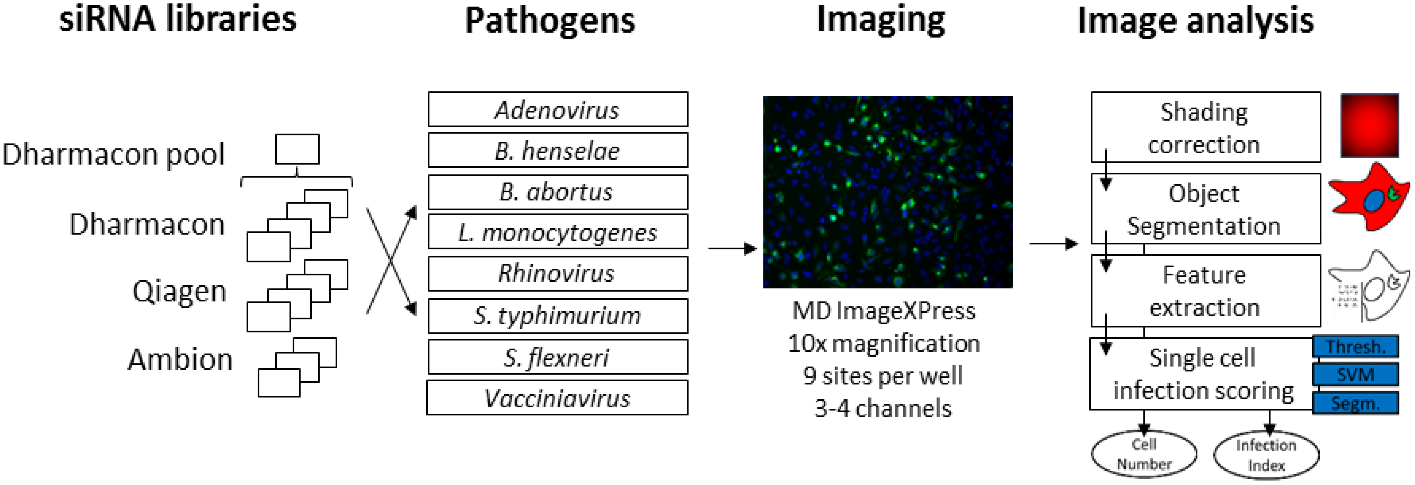
\includegraphics[width=0.95\textwidth]{infectx}
  \caption[InfectX RNAi data acquisition and analysis workflow.]{A total of 11 single \gls{sirna} libraries, pdroduced by 3 separate manufacturers, (4 from Dharmacon, 4 from Quiagen and 3 from Ambion), as well as one pooled library (Dharmacon) were screened with 8 pathogens. Plates were imaged under wide-field microscopes and the resulting images run through an image analysis pipeline. \citep{Ramo2014}.}
  \label{fig:infectx}
\end{figure}

The model system chosen for investigation is HeLa (ATCC CCL-2), the oldest and most wide spread human cell line and a proven system for studying infelicitous disease\footnote{Collected 60 years ago from a cervical adenocarcinoma, these epithelial cells have led to much insight into human cell biology. Prior to their discovery, attempts at growing human tissue in vitro were futile and development of protocols for sustaining cancerous human tissue was thought to hold great promise for cancer research. One of the early successes involving HeLa cells was the development a polio vaccine. For this endeavor, a large amount of human cells were needed and the installment of a production facility capable of meeting the high demand might have contributed significantly to the predominance of these cells. \citep{Masters2002}}. Culturing was performed at \SI{37}{\celsius}, under 5\% \ce{CO2} atmosphere for maintaining optimal pH, using \gls{dmem}  supplemented with 10\% inactivated \gls{fbs}, both supplied by Invitrogen.

While genome-wide \gls{sirna} screens were also produced within the InfectX framework, this report focuses on kinome-wide investigations. Introduced by \cite{Manning2002}, the term kinome refers to the subset of genes encoding protein kinases\footnote{Kinases are part of the larger enzymatic family of transferases and catalyze phosphorylation reactions of the form
\begin{equation}
  \ce{A\bond{-}O\bond{-}PO3^{-2} + H\bond{-}X\bond{-}B <=>> B\bond{-}X\bond{-}O\bond{-}PO3^{-2} + H\bond{-}O\bond{-}A} \label{eq:kinase}
\end{equation}
where A represents the donating (typically \gls{atp}) and B the accepting molecule. Kinases are further subdivided according to the type of acceptor which can be an alcohol, carboxy, nitrogenous or phosphate group, or in case of protein kinases, a tyrosine, serine, threonine or histidine residue.
\begin{align}
  \ce{A\bond{-}O\bond{-}B + H\bond{-}O\bond{-}PO3^{-2} &<=>> A\bond{-}O\bond{-}PO3^{-2} + H\bond{-}O\bond{-}B} \label{eq:phosphorylase} \\
  \ce{A\bond{-}O\bond{-}PO3^{-2} + H\bond{-}OH &<=>> A\bond{-}OH + H\bond{-}O\bond{-}PO3^{-2}} \label{eq:phosphatases}
\end{align}
Phosphorylases are a further group of transferases that involve phosphate but unlike kinases, they utilize inorganic phosphate sources (\ref{eq:phosphorylase}). Often phosphorylases are involved in breaking down biological polymers such as polysaccharides and polynucleotides. Finally, phosphatases catalyze the reverse reaction, the removal of a phosphate group (\ref{eq:phosphatases}).}. As phosphorylation reactions have been identified to constitute the most widespread signaling mechanism in eukaryotic cells, the set of 518 genes identified by \citeauthor{Manning2002} are a popular target for functional genomics studies. Up to 30\% of intracellular proteins may be phosphorylated, leading to 20000 phosphoprotein states, all regulated by expression of varyingly substrate specific kinases \citep{Johnson2005}. Due to the importance of kinases for cell behavior, they represent a major drug target in cancer therapeutics and might therefore also be attractive for \gls{hdt}.

In order to offset potential bias introduced by \gls{sirna} design paradigms employed by manufacturers, libraries from three different companies (Abion, Dharmacon and Qiagen) were obtained. To further account for the effect of \glspl{ote}, several \gls{sirna} sequences per target were used for both pooled and unpooled experiments. The Ambion Silencer Select Human Kinase siRNA Library V4 targets 710 genes of kinases and kinome-associated proteins with 3 sequences each, while the Qiagen HP OnGuard Human Kinase siRNA Set V4.1 comprises of 718 targets and 4 \glspl{sirna} per gene. The Dharmacon Human ON-TARGETplus siRNA Protein Kinase Libraries are designed with 715 genes in mind and are both available in 1 \gls{sirna} per well (unpooled) and 4 \glspl{sirna} per well (pooled) formats.

\begin{table}
  \centering
  \caption[Number of replicates performed for each of the pathogens and \gls{sirna} libraries.]{Number of replicates performed for each of the pathogens and \gls{sirna} libraries. The primary values indicate how many were performed in total while the value in parenthesis represents the number of screens that turned out to be unusable and had to be discarded. The effectively available number of replicates is the difference between the two. \citep{Ramo2014}}
  \label{tab:infectx-replicates}
  \footnotesize
  \begin{tabular}{L{0.2\linewidth}C{0.13\linewidth}C{0.13\linewidth}C{0.13\linewidth}C{0.15\linewidth}}
    Pathogen &
      Dharmacon (1x pooled) &
      Ambion (3x single) &
      Quiagen (4x single) &
      Dharmacon (4x single) \\
    \hline 
    \textit{B. abortus} &
      8 (1 rem.) &
      2 &
      1 &
      2 \\
    \textit{B. henselae} &
      5 (1 rem.) &
      4 (1 rem.) &
      2 (1 rem.) &
      1 \\
    \textit{L. monocytogenes} &
      4 &
      4 (2 rem.) &
      1 &
      1 \\
    \textit{S. flexneri} &
      6 (2 rem.) &
      2 &
      1 &
      1 \\
    \textit{S.} typhimurium &
      7 (4 rem.) &
      3 &
      1 &
      1 \\
    adenovirus &
      8 (1 rem.) &
      2 &
      1 &
      1 \\
    rhinovirus &
      8 (2 rem.) &
      2 &
      1 &
      1 \\
    vaccinia virus &
      2 (1 rem.) &
      2 &
      1 &
      1 \\
    \hline
  \end{tabular}
\end{table}

Depending on library and pathogen, screens were repeated 1--8 times (see table \ref{tab:infectx-replicates}). The primary values denote the total number of replicated performed and the values in parenthesis indicate the number of screens that had to be removed due to issues with transfection, weak signal intensities or usage of a protocol other than the one eventually agreed upon. The Dharmacon pooled screen was used for optimizing the assay procedures which is why for almost all pathogens some replicates had to be removed. The number of available screens is the difference between primary and parenthesized values.

\section{RNA Interference Protocols}
Central to the \gls{sirna} screens produced by InfectX was the effort to develop unified protocols for wet-tab experiments and subsequent analysis. While this approach was successfully implemented for many aspects, some deviations among the pathogens are inevitable, while others are intentionally developed to achieve similar phenotypes. Table \ref{tab:infectx-differences} summarizes some key parameters that vary between pathogens, which include seeded cell number, \gls{moi} and infection times, all optimized to yield infection rates that are of comparable magnitude. The target value for cell number was 1500 per well in order to create densely populated areas interspersed with some empty spaces, leading to cells living on colony edges and infection rates of 30--50\% were aimed for. Pathogen properties made it in some cases impossible th hit these goals and infection rate for \textit{B. abortus} remained low (\tilde 5\%), while being high in \textit{B. henselae} (\tilde 90\%) despite best efforts.

\setlength{\tabcolsep}{0.1em}
\begin{table}
  \begin{minipage}{\textwidth}
  \centering
  \caption[Differences in assay protocols among the 8 pathogens.]{Despite putting much emphasis on using identical protocols throughout all screens, some assay parameters were fine-tuned in order to obtain phenotypes such as infection and cell counts that are similar among the investigated pathogens. \citep{Ramo2014}}
  \label{tab:infectx-differences}
  \footnotesize
  \begin{tabular}{L{0.17\linewidth}C{0.09\linewidth}C{0.09\linewidth}C{0.09\linewidth}C{0.09\linewidth}C{0.09\linewidth}C{0.09\linewidth}C{0.10\linewidth}C{0.10\linewidth}}
    Pathogen &
      \mcrot{1}{l}{60}{Seeded cell number} &
      \mcrot{1}{l}{60}{\Acrshort{moi}} &
      \mcrot{1}{l}{60}{Pathogen entry time} &
      \mcrot{1}{l}{60}{Total infection time} &
      \mcrot{1}{l}{60}{DNA stain} &
      \mcrot{1}{l}{60}{Actin stain\footnote{Phalloidin-based actin stains were supplied by Dyomics and depending on absorption wavelength, different imaging channels were used: GFP for DY-495, RFP for DY-547 and Cy5 for DY-647.}} &
      \mcrot{1}{l}{60}{Pathogen stain} &
      \mcrot{1}{l}{60}{Additional stain\footnote{The Cy3 channel was used Alexa546, staining bacterially secreted InlC, while Cy5 was used for Alexa647, staining cellular \gls{il-8} during imaging.}} \\
    \hline 
    \textit{B. abortus} &
      500 &
      10000 &
      \SI{4}{\hour} &
      \SI{44}{\hour} &
      DAPI &
      DY-547 &
      GFP &
      - \\
    \textit{B. henselae} &
      300 &
      400 &
      \SI{24}{\hour} &
      \SI{24}{\hour} &
      DAPI &
      DY-547 &
      GFP &
      - \\
    \textit{L. monocytogenes} &
      600 &
      25 &
      \SI{1}{\hour} &
      \SI{5}{\hour} &
      DAPI &
      DY-647 &
      GFP &
      Alexa546 \\
    \textit{S. flexneri} &
      600 &
      15 &
      \SI{30}{\minute} &
      \SI{3.5}{\hour} &
      Hoechst &
      DY-495 &
      DsRed &
      Alexa647 \\
    \textit{S.} typhimurium &
      550 &
      80 &
      \SI{20}{\minute} &
      \SI{4}{\hour} &
      DAPI &
      DY-547 &
      GFP &
      - \\
    adenovirus &
      700 &
      0.1 &
      \SI{16}{\hour} &
      \SI{16}{\hour} &
      DAPI &
      DY-647 &
      GFP &
      - \\
    rhinovirus &
      1000 &
      8 &
      \SI{7}{\hour} &
      \SI{7}{\hour} &
      DAPI &
      DY-647 &
      GFP &
      - \\
    vaccinia virus &
      600 &
      0.125 &
      \SI{1}{\hour}\slash \SI{8}{\hour}\footnote{The two values stand for primary and secondary infection times, respectively. The same goes for pathogen dyes.} &
      \SI{24}{\hour} &
      Hoechst &
      DY-647 &
      GFP\slash RFP &
      - \\
  \end{tabular}
  \end{minipage}
\end{table}

The usage of control wells enables diagnosis of possible problems that may occur in RNAi screens, including cytotoxicity of \gls{sirna}, low transfection yields, failure of RNAi pathway induction, dominance of non-specific responses, and therefore should be embedded in every assay plate. Three types of control experiments are typically employed: positive, negative and mock (no \gls{sirna} treatment). Positive controls are used to confirm expected response, while negative controls help distinguish sequence specific from unspecific effects, and mock experiments help to establish a baseline \citep{Sittampalam2004}.

Positive controls ideally constitute of \glspl{sirna} with known effect on the assay under investigation and are therefore often unavailable beforehand. Instead, controls to check transfection efficiency and reporter quality are usually employed. One straightforward possibility for monitoring delivery is by targeting a gene that is vital to the cell. \Gls{kif11}, for example is a gene involved in cell cycle progression, the down-regulation of which is induces apoptosis. Furthermore there are mixtures of \glspl{sirna} available (e.g. AllStars Hs Cell Death Control siRNA by Qiagen) optimized for killing cells by targeting several ubiquitously expressed genes essential for cell survival. The downside of assessing transfection by killing cells is that a potentially toxic effect of the delivery mechanism itself may be masked. This can be mitigated by either performing negative control experiments (which should be done anyways) or by targeting housekeeping genes that are abundantly expressed but do not affect cell viability. Dharmacon suggests three such genes, \gls{ppib}, \gls{gapdh} and \gls{lmna}, for which they sell specially branded control \glspl{sirna} (as does Ambion).

Fluorescent dyes are also frequently employed in positive control experiments, typically by labeling \gls{sirna}, allowing for visual inspection of reagent localization within the cell (nuclear uptake indicates efficient transfection), or by targeting reporter genes. The latter method either allows for confirming that the reporting mechanism (usually expression of \gls{gfp} or luciferase) works as intended, or establishing that \gls{sirna} transfection was successful. Again, \gls{sirna} products targeting the commonly used reporter genes are readily available from manufacturers.

\renewcommand{\arraystretch}{1.1}
\setlength{\tabcolsep}{0.14em}
\begin{table}
\begin{minipage}{\textwidth}
  \centering
  \caption[Control experiments used in the different screens.]{Depending on screen type and pathogen, different genes were targeted for control experiments. Abbreviations: AU, Ambion unpooled; DP, Dharmacon pooled; DU, Dharmacon unpooled; and QU, Qiagen unpooled.}
  \label{tab:infectx-control}
  \footnotesize
  % latex table generated in R 3.2.0 by xtable 1.7-4 package
% Fri Aug  7 21:19:25 2015
\begin{tabular}{rllllllllllllllllllllllllllllllll}
  & \begin{sideways} Adeno AU \end{sideways} & \begin{sideways} Adeno DP \end{sideways} & \begin{sideways} Adeno DU \end{sideways} & \begin{sideways} Adeno QU \end{sideways} & \begin{sideways} \textit{Bartonella} AU \end{sideways} & \begin{sideways} \textit{Bartonella} DP \end{sideways} & \begin{sideways} \textit{Bartonella} DU \end{sideways} & \begin{sideways} \textit{Bartonella} QU \end{sideways} & \begin{sideways} \textit{Brucella} AU \end{sideways} & \begin{sideways} \textit{Brucella} DP \end{sideways} & \begin{sideways} \textit{Brucella} DU \end{sideways} & \begin{sideways} \textit{Brucella} QU \end{sideways} & \begin{sideways} \textit{Listeria} AU \end{sideways} & \begin{sideways} \textit{Listeria} DP \end{sideways} & \begin{sideways} \textit{Listeria} DU \end{sideways} & \begin{sideways} \textit{Listeria} QU \end{sideways} & \begin{sideways} Rhino AU \end{sideways} & \begin{sideways} Rhino DP \end{sideways} & \begin{sideways} Rhino DU \end{sideways} & \begin{sideways} Rhino QU \end{sideways} & \begin{sideways} \textit{Salmonella} AU \end{sideways} & \begin{sideways} \textit{Salmonella} DP \end{sideways} & \begin{sideways} \textit{Salmonella} DU \end{sideways} & \begin{sideways} \textit{Salmonella} QU \end{sideways} & \begin{sideways} \textit{Shigella} AU \end{sideways} & \begin{sideways} \textit{Shigella} DP \end{sideways} & \begin{sideways} \textit{Shigella} DU \end{sideways} & \begin{sideways} \textit{Shigella} QU \end{sideways} & \begin{sideways} Vaccinia AU \end{sideways} & \begin{sideways} Vaccinia DP \end{sideways} & \begin{sideways} Vaccinia DU \end{sideways} & \begin{sideways} Vaccinia QU \end{sideways} \\ 
  \hline
ARF1 &  &  &  &  &  &  &  &  &  &  &  &  &  &  &  &  &  &  &  &  &  &  &  &  &  &  & \checkmark &  &  &  &  &  \\ 
  ARPC3 & \checkmark & \checkmark & \checkmark & \checkmark & \checkmark & \checkmark & \checkmark & \checkmark & \checkmark & \checkmark & \checkmark & \checkmark & \checkmark & \checkmark & \checkmark & \checkmark & \checkmark & \checkmark & \checkmark & \checkmark & \checkmark & \checkmark & \checkmark & \checkmark & \checkmark & \checkmark & \checkmark & \checkmark & \checkmark & \checkmark & \checkmark & \checkmark \\ 
  ATP6V1A & \checkmark & \checkmark & \checkmark & \checkmark & \checkmark & \checkmark & \checkmark & \checkmark & \checkmark & \checkmark & \checkmark & \checkmark & \checkmark & \checkmark & \checkmark & \checkmark & \checkmark & \checkmark & \checkmark & \checkmark & \checkmark & \checkmark & \checkmark & \checkmark & \checkmark & \checkmark & \checkmark & \checkmark & \checkmark & \checkmark & \checkmark & \checkmark \\ 
  Abi1 &  &  &  & \checkmark &  &  &  & \checkmark &  &  &  & \checkmark &  &  &  & \checkmark &  &  &  & \checkmark &  &  &  & \checkmark &  &  &  & \checkmark &  &  &  & \checkmark \\ 
  CBL &  &  &  &  &  &  &  &  &  &  &  &  &  & \checkmark & \checkmark &  &  &  &  &  &  &  &  &  &  &  &  &  &  &  &  &  \\ 
  CDC42 & \checkmark & \checkmark & \checkmark & \checkmark & \checkmark & \checkmark & \checkmark &  & \checkmark & \checkmark & \checkmark &  & \checkmark & \checkmark & \checkmark &  & \checkmark & \checkmark & \checkmark & \checkmark & \checkmark & \checkmark & \checkmark &  & \checkmark & \checkmark & \checkmark &  & \checkmark & \checkmark & \checkmark & \checkmark \\ 
  CDH4 &  &  &  & \checkmark &  &  &  & \checkmark &  &  &  & \checkmark &  &  &  & \checkmark &  &  &  & \checkmark &  &  &  & \checkmark &  &  &  & \checkmark &  &  &  & \checkmark \\ 
  CFL1 &  &  &  &  &  &  &  &  &  &  &  &  &  &  &  &  &  &  &  &  &  &  & \checkmark &  &  &  &  &  &  &  &  &  \\ 
  CHUK &  &  &  &  &  &  &  &  &  &  &  &  &  &  &  &  &  &  &  &  &  &  &  &  &  &  & \checkmark &  &  &  &  &  \\ 
  CLTC &  &  &  &  &  &  &  &  &  &  &  &  &  & \checkmark & \checkmark &  &  &  &  &  &  &  &  &  &  &  &  &  &  &  &  &  \\ 
  DNM2 &  &  &  &  &  &  &  &  &  &  &  &  &  & \checkmark & \checkmark &  &  &  &  &  &  &  &  &  &  &  &  &  &  &  &  &  \\ 
  FRAP1 &  &  & \checkmark & \checkmark &  &  &  & \checkmark &  &  &  & \checkmark &  &  &  & \checkmark &  &  & \checkmark & \checkmark &  &  &  & \checkmark &  &  &  & \checkmark &  &  &  & \checkmark \\ 
  GFP 1\footnote{\label{fn:gfp}GFP targeting \gls{sirna} sequences are provided by Ambion (Ambion Silencer eGFP; GFP 1) and Dharmacon (GFP Duplex III; GFP 2).} & \checkmark &  &  &  & \checkmark &  &  &  & \checkmark &  &  &  & \checkmark &  &  &  & \checkmark &  &  &  & \checkmark &  &  &  & \checkmark &  &  &  & \checkmark &  &  &  \\ 
  GFP 2\textsuperscript{\ref{fn:gfp}} & \checkmark & \checkmark & \checkmark & \checkmark &  & \checkmark & \checkmark & \checkmark &  & \checkmark & \checkmark & \checkmark &  & \checkmark & \checkmark & \checkmark & \checkmark & \checkmark & \checkmark & \checkmark &  & \checkmark & \checkmark & \checkmark &  & \checkmark & \checkmark & \checkmark &  & \checkmark & \checkmark & \checkmark \\ 
  ITGAV &  &  &  &  &  &  &  &  &  &  &  &  &  &  &  &  &  &  &  &  &  &  & \checkmark &  &  &  &  &  &  &  &  &  \\ 
  ITGB1 &  &  &  & \checkmark &  &  & \checkmark & \checkmark &  &  & \checkmark & \checkmark &  &  &  & \checkmark &  &  &  & \checkmark &  &  &  & \checkmark &  &  &  & \checkmark &  &  &  & \checkmark \\ 
  Kif11 & \checkmark & \checkmark & \checkmark & \checkmark & \checkmark & \checkmark & \checkmark & \checkmark & \checkmark & \checkmark & \checkmark & \checkmark & \checkmark & \checkmark & \checkmark & \checkmark & \checkmark & \checkmark & \checkmark & \checkmark & \checkmark & \checkmark & \checkmark & \checkmark & \checkmark & \checkmark & \checkmark & \checkmark & \checkmark & \checkmark & \checkmark & \checkmark \\ 
  Kill\footnote{A positive control cell killer is provided by Qiagen (AllStars Hs Cell Death Control)} &  &  &  & \checkmark &  &  &  & \checkmark &  &  &  & \checkmark &  &  &  & \checkmark &  &  &  & \checkmark &  &  &  & \checkmark &  &  &  & \checkmark &  &  &  & \checkmark \\ 
  MAP3K7 &  &  &  & \checkmark &  &  &  & \checkmark &  &  &  & \checkmark &  &  &  & \checkmark &  &  &  & \checkmark &  &  &  & \checkmark &  &  & \checkmark & \checkmark &  &  &  & \checkmark \\ 
  MET &  &  &  & \checkmark &  &  &  & \checkmark &  &  &  & \checkmark &  & \checkmark & \checkmark & \checkmark &  &  &  & \checkmark &  &  &  & \checkmark &  &  &  & \checkmark &  &  &  & \checkmark \\ 
  MOCK & \checkmark & \checkmark & \checkmark & \checkmark & \checkmark & \checkmark & \checkmark & \checkmark & \checkmark & \checkmark & \checkmark & \checkmark & \checkmark & \checkmark & \checkmark & \checkmark & \checkmark & \checkmark & \checkmark & \checkmark & \checkmark & \checkmark & \checkmark & \checkmark & \checkmark & \checkmark & \checkmark & \checkmark & \checkmark & \checkmark & \checkmark & \checkmark \\ 
  NOD1 &  &  &  &  &  &  &  &  &  &  &  &  &  &  &  &  &  &  &  &  &  &  &  &  &  &  & \checkmark &  &  &  &  &  \\ 
  PAK1 &  &  &  &  &  &  &  &  &  &  &  &  &  &  &  &  &  &  &  &  &  &  &  &  &  &  &  &  &  &  & \checkmark & \checkmark \\ 
  PI4KA &  &  &  &  &  &  &  &  &  &  &  &  &  &  &  &  &  &  &  &  &  &  &  &  &  &  & \checkmark &  &  &  &  &  \\ 
  PI4KB &  &  &  & \checkmark &  &  &  & \checkmark &  &  &  & \checkmark &  &  &  & \checkmark &  &  &  & \checkmark &  &  &  & \checkmark &  &  &  & \checkmark &  &  &  & \checkmark \\ 
  PIK3R1 &  &  &  &  &  &  &  &  &  &  &  &  &  & \checkmark & \checkmark &  &  &  &  &  &  &  &  &  &  &  &  &  &  &  &  &  \\ 
  PRKCA &  &  & \checkmark & \checkmark &  &  &  &  &  &  &  &  &  &  &  &  &  &  & \checkmark & \checkmark &  &  &  &  &  &  &  &  &  &  &  &  \\ 
  PSMA6 &  &  &  &  &  &  &  &  &  &  &  &  &  &  &  &  &  &  &  &  &  &  &  &  &  &  &  &  &  &  & \checkmark & \checkmark \\ 
  PSMC3 &  &  &  & \checkmark &  &  &  & \checkmark &  &  &  & \checkmark &  &  &  & \checkmark &  &  &  & \checkmark &  &  &  & \checkmark &  &  &  & \checkmark &  &  & \checkmark & \checkmark \\ 
  PXN &  &  & \checkmark & \checkmark &  &  & \checkmark & \checkmark &  &  & \checkmark & \checkmark &  &  &  & \checkmark &  &  & \checkmark & \checkmark &  &  &  & \checkmark &  &  &  & \checkmark &  &  &  & \checkmark \\ 
  RAB7A &  &  &  &  &  &  &  &  &  &  &  &  &  &  &  &  &  &  &  &  &  &  & \checkmark &  &  &  &  &  &  &  &  &  \\ 
  RAC1 &  &  & \checkmark & \checkmark &  &  & \checkmark &  &  &  & \checkmark &  &  &  &  &  &  &  & \checkmark & \checkmark &  &  &  &  &  &  &  &  &  &  & \checkmark & \checkmark \\ 
  Rab2 &  &  &  &  &  &  & \checkmark &  &  &  & \checkmark &  &  &  &  &  &  &  &  &  &  &  &  &  &  &  &  &  &  &  &  &  \\ 
  SNX9 &  &  & \checkmark & \checkmark &  &  &  &  &  &  &  &  &  &  &  &  &  &  & \checkmark & \checkmark &  &  &  &  &  &  &  &  &  &  &  &  \\ 
  Scra 1\footnote{\label{fn:scram}Scrambled \gls{sirna} sequences are provided by Ambion (Silencer Select Negative Control; Scra 1) and Dharmacon (ON-TARGETplus Non-targeting Control; Scra 2).} & \checkmark &  &  &  & \checkmark &  &  &  & \checkmark &  &  &  & \checkmark &  &  &  & \checkmark &  &  &  & \checkmark &  &  &  & \checkmark &  &  &  & \checkmark &  &  &  \\ 
  Scra 2\textsuperscript{\ref{fn:scram}} & \checkmark & \checkmark & \checkmark & \checkmark &  & \checkmark & \checkmark & \checkmark &  & \checkmark & \checkmark & \checkmark &  & \checkmark & \checkmark & \checkmark & \checkmark & \checkmark & \checkmark & \checkmark &  & \checkmark & \checkmark & \checkmark &  & \checkmark & \checkmark & \checkmark &  & \checkmark & \checkmark & \checkmark \\ 
  TLN1 &  &  &  &  &  &  & \checkmark &  &  &  & \checkmark &  &  &  &  &  &  &  &  &  &  &  &  &  &  &  &  &  &  &  &  &  \\ 
  TSG101 &  &  &  &  &  &  &  &  &  &  &  &  &  &  &  &  &  &  &  &  &  &  &  &  &  &  &  &  &  &  & \checkmark & \checkmark \\ 
  \end{tabular}


\end{minipage}
\end{table}

Negative controls should lack homology with known targets in order to separate non-specific effects from sequence specific silencing. Such \glspl{sirna} are therefore engineered to contain a passenger strand seed region (the first 2--6 nt from the 5' end) that matches no known gene and and generally have poor overall sequence identity between passenger strand and any known gene. One way of generating such a sequence is taking an assay \gls{sirna} and randomizing the order of nucleotides while keeping the nucleotide composition unchanged (i.e. scrambling the sequence). Multiple proposals are usually generated and subsequently checked for applicability by sequence alignment to the target genome. While scrambling has the advantage that a possible effect of nucleotide composition is removed, it is infeasible for large-scale screens and often a set of predefined sequences sold by manufacturers (for example Silencer Select Negative Control from Ambion, ON-TARGETplus Non-targeting Control siRNAs from Dharamcon or AllStars Negative Control siRNA from Qiagen) is used instead (while still being called scrambled controls). 

Table \ref{tab:infectx-control} lists the \gls{sirna} control experiments that were performed throughout all screens and indicates the set of controls each screen contains. Common to all pathogens and all libraries are the previously mentioned positive control Kif11, one of two \gls{gfp} targeting sequences, scrambled \glspl{sirna}, as well as mock experiments. Additionally, several controls for general infection mechanisms were included in most screens, including ATP6V1A (a \ce{H^+} transporting ATPase, responsible for acidification of endocytic and lysosomal vesicles), ARPC3 (\acrshort{arp23}), and \gls{cdc-42}, both part of actin-dependent processes surrounding pathogen uptake and \gls{abm}. Some controls however are specific to a subgroup of pathogens or single pathogens and include the following (grouped by pathogen).
\begin{description}[leftmargin=0.5cm]
\item[\textit{Bartonella}\slash \textit{Brucella}:] The small GTPase Rab2 is required for anterograde \gls{er}--Golgi transport, capable of interacting with RicA of \textit{B. abortus} \citep{DeBarsy2011} and TLN1 (talin 1) has been determined to be necessary for invasome formation in \textit{B. henselae} infection via \textbeta\textsubscript{1} signaling \citep{Truttmann2011}.
\item[\textit{Listeria}:] During endocytosis of \textit{L. monocytogenes}, the ubiqutin ligase Cbl is a recruited to the site of entry and seems to be involved in InlB mediated, clathrin dependent (CLTC encodes the heavy chain 1 component of clathrin) bacterial uptake \citep{Veiga2005}. DNM2 (dynamin-2) is a further protein involved in host entry and PIK3R1 is a phosphatidylinositol 3-kinase, downstream to Met, the cellular receptor to InlB.
\item[\textit{Salmonella}:] The actin-modulating protein CFL1 (cofilin-1), responsible for actin depolymerization, the cellular integrin receptor ITGAV and RAB7A, a small GTPase that regulates vesicular trafficking, have all been shown to be hits in a salmonella invasion screen \citep{Misselwitz2011}.
\item[\textit{Shigella}:] Down regulation of ARF1 (a \gls{gtp} binding protein involved in vesicle trafficking) and phosphatidylinositol 4-kinase PI4KA has been suspected of interfering with pathogen entry, while suppression of CHUK\slash NOD1 (both involved in \gls{nf-kb} signaling) may inhibit \gls{il-8} production by uninfected bystander cells, thereby possibly promoting infection \citep{Kasper2012}. 
\item[Adenovirus\slash rhinovirus:] SNX9 regulates dynamin assembly and is therefore crucial to viral endocytosis and PRKCA is a Ser-\slash Thr-specific protein kinase responsible for a wide array of regulatory signals. PRKCA might be involved in influenza virion buddying and has been implicated in playing a role in intracellular proliferation of hepatitis \citep{Kanehisa2000}.
\item[Vaccinia virus:] The Ser-\slash Thr-specific protein kinase PRKCA is targeted by \gls{cdc-42}\slash \gls{rac-1} and has been shown to be required for \gls{mv} entry \citep{Mercer2008}. Up-regulation of PSMA6 (a proteasome complex component) enables evasion of intracellular immune surveillance \citep{Zhou2014} and TSG101, ubiquitin-conjugating enzyme, hampers \gls{ev} production \citep{Honeychurch2007}. 
\end{description}

Many of these pathogen specific positive control targets are not well established and while some have been previously been identified and validated, others represent best guesses and might not serve their purpose particularly well. Controls wells are typically located at the plate border (rows A and P; columns 1, 2, 23 and 24) and the different control experiments were replicated multiple times on each plate.

For all screens, \gls{sirna} transfection was carried out by adding \SI{25}{\micro\litre} of RNAi\-MAX\slash DMEM (\SI{0.1}{\micro\litre}\slash \SI{24.9}{\micro\litre}) transfection agent to \SI{1.6}{\pico\mol} siRNA diluted in \SI{5}{\micro\litre} RNase-free \ce{ddH2O} contained in each of the 384 wells per screening plate. After \SI{1}{\hour} incubation at room temperature, the required number of cells were added (see table \ref{tab:infectx-differences}), suspended in \SI{50}{\micro\litre} DMEM\slash 16\% \gls{fbs}. Plates were subsequently incubated for \SI{72}{\hour} at \SI{37}{\celsius} and 5\% \ce{CO2}, followed by the pathogen specific infection procedure (see section \ref{sec:pathogen-protocols} for details). Following infection, cells were fixed in \gls{pfa} and stained for DNA, F-actin and additional pathogen specific markers (see table \ref{tab:infectx-differences}). Plates were sealed prior to imaging.

\section{Image Acquisition and Data Processing}
Imaging was performed both at the University of Basel and the Light Microscopy and Screening Center of ETH Z\"urich, using ImageXpress micro (IXM) HCS wide-field microscopes from Molecular Devices, equipped with Thermo Scientific CataLyst Express robotic plate handlers capable of storing and serving up to 45 plates. Lumencor Spectra X solid-state light engines (LED light sources), 10x S Fluor objective lenses by Nikon with a numerical aperture of 0.45 and Photometrics CoolSNAP HQ 14-bit CCD cameras, resolving $1392 \times 1040$ pixels (individual pixel size of $\SI{6.45}{\micro\meter} \times \SI{6.45}{\micro\meter}$), complete the hardware setup. Channel selection is assay specific and stain dependent Semrock filters (DAPI\slash Hoechst, GFP\slash FITC\slash Alexa488, Cy3, Cy5, Quadband DAPI-GFP-mCherry-Cy5) are employed (see table \ref{tab:infectx-differences} for details).

Wells are divided into $3 \times 3$ grids for most plates while some $2 \times 3$ site images exist too, with no spacing and no overlap, and Molecular Devices MetaXpress High-Content Image Acquisition and Analysis Software was used for recording images. Software parameters include no gain, well bottom as autofocus target, site-specific autofocusing, enabling of laser-based focusing and no shading correction. For each imaging channel, focus Z-offset was selected manually and exposure time was automatically calculated. In cases of poor dynamic range or overexposure, manual correction to exposure time was applied. Upon imaging, data was transferred to iBrain2\slash screeningBee \citep{Rouilly2012} for further processing.

\subsection{Data Handling (iBrain2\slash screeningBee)}
In case of microscopy based \gls{sirna} screening experiments, a complex task of data handling and processing follows the imaging stage. A wealth of data is generated by imaging devices\footnote{A genome-wide screen (\tilde 27000 individual experiments) in 384 well format involves 70--100 plates depending on the number of controls per plate. Each plate yields 10000--14000 images (384 wells, 9 sites and 3--4 channels), leading to 700000--1400000 individual images and requiring multiple terabytes of storage.} which has to be accessibly and redundantly stored. Furthermore, analysis of image data is a processing intensive task that quickly becomes reliant on \gls{hpc} resources, entailing specialized requirements due to the oftentimes shared and centralized nature of such systems. The authors of iBrain2 summarize the key steps in RNAi \gls{hcs} data processing as follows \citep{Rouilly2012}:
\begin{enumerate}
\item \textbf{Data acquisition.} The raw data of \gls{sirna} screens is produced as digital images by microscopy. Acqusition times of several hours per plate are typical and a single plate yields \tilde \SI{20}{\giga\byte} of data.
\item \textbf{Permanent storage.} Due to infeasibility of re-screening plates, all raw data has to be stored in a sufficiently redundant manner. Furthermore, the permanent data store has to be able to serve portions of the dataset quickly and efficiently.
\item \textbf{Temporary data staging to \gls{hpc}.} In order for the compute cluster not to be bound by network latency, it is often necessary to stage the data to be analyzed to local scratch space. This step becomes superfluous whenever the permanent storage system is directly integrated in the cluster's high-speed network.
\item \textbf{Data analysis.} Many aspects of processing a large number of images are embarrassingly parallel and a cluster environment is ideally suited to tackle this computation intensive task.
\item \textbf{Permanent storage of results.} Some results produced by the analysis procedure will be saved back to the permanent storage system. While it may be sensible to save storage space and carry out some procedures on the fly, this is not feasible for all analysis routines.
\item \textbf{Publication and archiving.} Upon completion of the project, some data will be made availably publicly and all data worth keeping is moved to an archival system capable of cheap long-term storage where quick retrieval is unimportant.
\end{enumerate}

The requirements outlined above led to the development of iBrain2 as a modular workflow manager capable of setting up reproducible procedures. The software is implemented in Java and uses an XML-based format for defining workflows. Furthermore, it interfaces with other open source projects, such as openBIS \citep{Bauch2011} which can be used as storage system and CellProfiler \citep{Carpenter2006,Kamentsky2011}, a popular tool for analyzing cell based image material. Within InfectX, not iBrain2 itself is used, but a derivative thereof called screeningBee, featuring tighter openBIS integration and a large set of CellProfiler extensions.

\subsection{Image Analysis (CellProfiler)}
Prior to the development and release of CellProfiler in 2006, large-scale screens were routinely evaluated though tedious and labor intensive visual inspection by expert biologists. While humans are able to perceive and contextualize image data in ways that computers still struggle to emulate, a lot of detail is lost though human interpretation. Small differences are hard to spot, leading to subtle patterns being missed and humans focus on a handful of features, not being able to take into account the plethora of information encoded in crowded images. Furthermore, human study of image data leads to qualitative evaluations, while computational analysis yields a potentially large number of quantitative measures. Lastly and perhaps most importantly, human based assessment of imagery coming from a project the size of InfectX is simply infeasible. In the words of \citeauthor{Carpenter2006}, the authors of CellProfiler, consequences of implementing computational image analysis for \gls{hts} are as follows:

\begin{quote}
With the successful application of sophisticated image analysis methods, the bottleneck of image-based genome-wide screens is now moving downstream to data visualization, exploration, and statistical analysis in order to accommodate the number and richness of measurements that result from image-based genome-wide assays.
\end{quote}

CellProfiler is an open-source software solution catering to the needs of \gls{hts} screening initiatives and providing a customizable, modular platform for cellular image analysis. CellProfiler processing is based on modules which are placed in sequential to form a pipeline, usually starting out with image processing, followed by object identification and concluded by calculation of feature measurements on these objects. The pipeline's modules and settings can be saved to a configuration file, in order to ensure reproducibility and transferability of workflows. The original version of CellProfiler was written in MATLAB and a more recent version 2 has been ported to python. InfectX procedures are based on version 1 \citep{Carpenter2006}.

The InfectX image analysis routine starts out with metadata collection and image quality assessment modules, followed by shading correction. Detecting out of focus images, wells that show signs of experimental error or problematic plates, however is still largely carried out by humans. Position dependent illumination and sensor inhomogeneities need to be corrected for, as they lead to decreased sensitivity in darker areas and make comparison of intensity based features between objects belonging to different areas of the image problematic.

Shading correction, while offered by a default module of CellProfiler, is implemented in a module developed specifically for InfectX. A shading model is generated per microscope, lamp, channel, pathogen and assay which can simply be applied to all corresponding images. This reduces the computational complexity of shading correction significantly and avoids errors associated with an automated procedure being applied to a diverse range of instances. Shading models are produced by overlaying images and calculating histograms per pixel position, yielding robust estimates for foreground intensities and by fixed offsetting, also estimates for background intensities. Subsequently, a foreground model is calculated and applied, leading to conservatively corrected images. With only little shading remaining, reliable object segmentation is possible, the result of which are used to calculate a further, final shading model based on pixel histograms and average object intensities.

Illumination corrected images are stitched together, channel separated and forwarded to CellProfiler modules for segmentation and feature calculation. Cell identification is a hard problem, especially if clumps are present. Whenever objects are present that can easily be identified, such as nuclei if DNA was stained, these are identified first (primary objects), facilitating identification of secondary objects, e.g. cells. In case of clumped cells, a three step algorithm is employed: clumps are recognized, then the dividing lines are defined and finally, some resulting objects may be removed or merged based on measurements such as size or shape.

Several modules developed in-house are used during the feature extraction stage, extending CellProfiler functionality to specific requirements including invasome and bacterial aggregate detection, more efficient neighbor feature measurement and collection of various properties per sub-cellular object. The features calculated by the CellProfiler pipeline are explored more in-depth in section \ref{sec:scf-data}. All results produced by image analysis are saved to an openBIS instance.

\begin{figure}
  \centering
  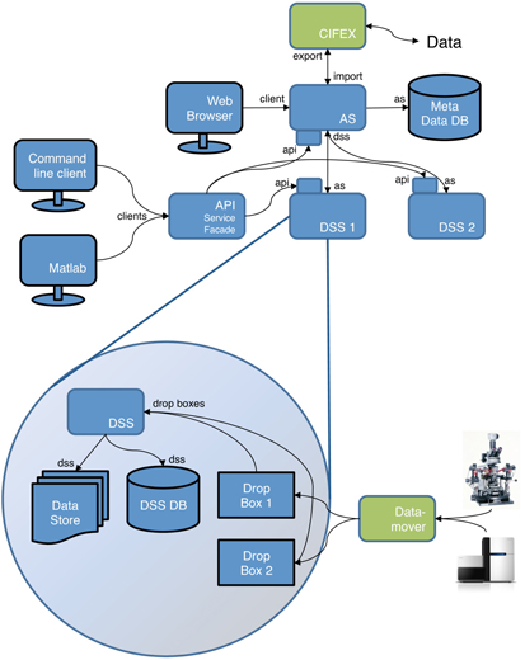
\includegraphics[width=0.7\textwidth]{openbis}
  \caption[Overview of the openBIS architecture and a more in-depth look at the data storage implementation.]{An openBIS instance is deployed as a service consisting of an application server (AS) and one or more data store servers (DSSs). At both levels, clients can interact with the system to query, fetch or deposit data. \citep{Bauch2011}.}
  \label{fig:openbis}
\end{figure}

\subsection{User Accessible Data Storage (OpenBIS)}
The authors of openBIS (open Biology Information System) argue that the availability of a domain specific information management system plays an important role in data-driven biological research, serving as a basis for management of large amounts of experimental data and acting as both a source and a sink for analysis procedures. Furthermore, such a system should provide a user interface capable of visualizing complex dependency structures and a set of \glspl{api} for accessing the stored data programmatically \citep{Bauch2011}. Finally, it should be possible to make a subset of the data available to the public, providing a simplified interface of the browsing and searching capabilities.

In order for openBIS to be applicable to the broad range of scenarios it is intended for, extensibility and transparent interfaces are paramount, as is scalability and performance. To address the latter aspect, separation of bulk data from metadata is a guiding principle. Both ingestion of high-throughput, high-content data as well as serving it to users and analysis routines is CPU, I/O and network intensive and therefore should not be performed on the same system as user-facing metadata queries which only deals with comparably inexpensive tasks that scale well. Additionally, scalability requires that bulk data storage may be distributed among several systems.

With these requirements in mind, openBIS is designed to consist of an \gls{as}, dealing with metadata, serving user queries such as searches and visualizing dependencies via the browser based graphical user interface, as well as one or several \glspl{dss} that handle the bulk data. Communication between the two layers is asynchronous.

All datasets in openBIS are immutable. While this is potentially wasteful in terms is storage resources, it can be argued that storage space is cheap and such an architecture improves traceability of constant evolution of analysis procedures and corresponding results. Datasets are subject to a hierarchical structure paradigm consisting of the entities \begin{enumerate*}[label=\itshape (\arabic*)] \item\textit{Data Space}, \item\textit{Project}, \item\textit{Experiment}, and \item\textit{Sample} \end{enumerate*}. In the example of \gls{hts} data, a sample represents a plate and associated datasets include raw images, feature measurements and infection scores. Metadata can be provided either in unstructured form which is handled as attachments associated with project, experiment or sample entities, or as structured objects (consisting of name, label, description and value) that are linked to experiments, samples and datasets.

Data storage by a \gls{dss} follows a hybrid model consisting of a relational database, storing index information, file metadata and selected results, in addition to flat-file data store which can be distributed between several file systems. Management of fill state of the associated storage shares and data distribution is all managed by the individual \glspl{dss}. Some data presentation task handled by \glspl{dss} include data visualizations such as plate heatmaps and assembly of multichannel images, as well as overlay of analysis results (e.g. segmentation).

Ingestion of new data can either be triggered by web import, custom software talking to the corresponding \gls{api} or simply by adding to folders that are monitored by a \gls{dss} as dropboxes. Responding to write activity, the highly customizable ETL (extract, transform, load) routine extracts metadata, creates datasets annotated with metadata in the \gls{as} database, links them to the appropriate entities and adds the new datasets to the data store. Export of data is either browser based or can be handled by provided command line tools, accessing openBIS via a Java service facade. Two separately designed tools are integrated for used with openBIS: CIFEX and Datamover. The former enables browser based transfer of large files and supports interruption  of transfers as well as checksumming for file integrity, while the latter can be used to automatically transfer data off of an instrument computer into a dropbox folder via SSH or rsync protocols.

\section{Single Cell Feature Data}
\label{sec:scf-data}
The set of accessible single cell features varies among screens and pathogens to some extent. While there are some general features, such as geometry, intensity and texture of nuclear and cellular objects available for every plate dataset, others, including invasome and \gls{il-8} features are specific to a subset of the pathogens, while others still, such as certain neighbor features or Vononoi cell segmentation were only recently added to the feature extraction pipeline and therefore have not yet been calculated for all screens. Such discrepancies are not treated by this overview which focuses on general aspects of currently available single cell features.

Nomenclature of single cell features follows a hierarchical pattern consisting of an object specifier, a measurement group, the measurement name itself and the imaging channel it was applied to, as follows:
\begin{center}
\texttt{<object>.<group>\_<measurement>\_<channel>}
\texttt{Cells.Intensity\_MedianUpperTenPercentIntensity\_CorrDNA}
\end{center}
In the above example, the measured objects are cells, the feature is of intensity type, the feature name indicates that it represents the mean of intensities above the upper decile and the channel description reveals that DNA stain values are used. Throughout the different screens, 14 single cell feature objects are available:

\begin{figure}
  \centering
  \includegraphics[width=0.95\textwidth]{segmentation}
  \caption[Object detection of nuclei, perinuclei, Voronoi cells and cell bodies along with potential pitfalls.]{Object identification is started with easily recognizable nuclei, which become primary objects and serving as basis for detecting secondary objects. Problems with nuclei detection include superfluous splitting (a) and failure to separate some touching objects (c). Mostly results are acceptable and some touching nuclei are correctly separated (b). Perinuclei extend the nuclear border and therefore suffer from problems introduced in nuclear recognition. Further issues include overlap with extracellular space (d) and small perinuclear area in densely populated areas (e). Voronoi cells further extend the nuclear area and often grow beyond cell boundaries (f). Finally, cell segmentation is a hard problem due to irregular shapes, variability in size and inhomogeneities in actin distribution (h). Results suffer from falsely identified nuclei (g and i).}
  \label{fig:segmentation}
\end{figure}

\begin{description}[leftmargin=0.5cm]
\item[Nuclei:] Using the DNA channel, nucleus recognition is fairly accurate owing to generally uniform morphology of nuclei, uniform distribution of DNA and good contrast of DNA staining. The current implementation for segmentation is based on Otsu's method which converts a monochromatic image into a binary image by finding an appropriate threshold, effectively separating foreground from background. Objects that have an Euler characteristic $\chi \le 0$ are filled and apparently clumped objects are split. Finally, objects outside of an allowed size range are discarded (mostly dust particles which are too big and pathogen DNA which yields objects that are too small). Nuclei represent primary objects with serve as basis for the detection of secondary objects (see figure \ref{fig:segmentation}, A).
\item[PeriNuclei:] The perinuclear region is defined as an extension of the nuclear border by 8 pixels and removal of the nucleus itself. As some pathogens establish their replicatory niche in this region it lends itself to closer investigation. Furthermore the border is only dependent on the reliably established nuclear object. Potential pitfalls include extension of the perinuclear region into extracellular space or neighboring cell when the nucleus is located close to the plasma membrane, as well as reduced area whenever cells are clustered, as perinuclear regions may not overlap (see figure \ref{fig:segmentation}, B).
\item[VoronoiCells:] Simultaneously extending all nuclei by maximally 24 pixels or until a neighboring border is met leads to Voronoi cells. This type of defining cell bodies is very prone to extending into extracellular space, as the actin channel is not taken into account (see figure \ref{fig:segmentation}, C).
\item[Cells:] The cell body border is determined by propagation segmentation based on thresholding. Starting from the nucleus, the cytoplasmic region is extended until the intensity gradient changes abruptly, indicating either the beginning of background, or the boundary to a neighboring cell. Non-uniform actin intensity patterns, irregular shape, large variability in size and frequent touching of neighbors makes this a hard problem and results can be unreliable. Common to all secondary objects, errors in determining primary objects will propagate and lead to cells erroneously being cut up or aggregated. Furthermore, borders to neighbors are frequently not determined correctly, but significant discrepancies among human expert labeling are to be expected in such situations as well (see figure \ref{fig:segmentation}, D).
\item[ExpandedNuclei:] Serving as precursors to PeriNuclei objects, these objects are not further quantified and only have coordinates and number of perinuclear children (almost exclusively 1) associated.
\item[Bacteria/Viruses/Pathogen:] Due to the heterogeneity between pathogens, detection is assay specific. Generally, pathogens are primary objects and not derived of cell nuclei. In \textit{Bartonella} and \textit{Brucella} screens, large and small pathogen clusters are segmented using Otsu's method on the pathogen channel. Individual bacteria in \textit{Listeria} screens, \glspl{scv} in \textit{Salmonella} screens and small\slash medium pathogen clusters in both \textit{Shigella} and rhinovirus screens are identified using wavelet decomposition of the pathogen channel, while for adenovirus screens, detection of large pathogen aggregates relies on propagation outwards from nuclei, much like cell body identification but using the pathogen channel. For vaccinia virus, direct pathogen segmentation is currently not possible.
\item[IntBacteria/ExtBacteria:] In \textit{Bartonella} assays, different stains were used for intracellular (\acrshort{gfp}) and extracellular (Cy5) bacteria which consequently can be distinguished during image analysis. This is helpful to prevent bacteria the are sit on top or below a cell from being considered intracellularly located.
\item[BlobBacteria:] Specific to \textit{Brucella} screens, these large bacterial aggregates do not have any real measurements associated, except coordinates.

\begin{figure}
  \centering
  \includegraphics[width=0.95\textwidth]{actin-features}
  \caption[Detection of two actin based structures, CometTails and Invasomes.]{Both CometTails and Invasomes are detected on actin channels, which poses difficulties due to noisy background. Invasomes are characterized by their ring-shaped morphology (a), while CometTails appear as actin streaks (c). Currently invasome detection yields many false-positives (b).}
  \label{fig:actin-features}
\end{figure}

\item[Invasomes:] As one of two internalization structures in \textit{Bartonella} infection, invasomes are characterized as actin surrounded large bacterial aggregates. Exploiting this morphology, the current invasome detection uses a ring template to search the actin channel for candidates and exploits the intensity difference to the cell mean for confirmation. Unfortunately, this yields many false positives. Improvements are being discussed but have yet to be implemented (see figure \ref{fig:actin-features}, A).
\item[IL8:] In \textit{Shigella} assays, cellular \gls{il-8} was stained in order to study proinflammatory response of uninfected bystander cells. Due to these objects having their own channel, segmentation is fairly straightforward.
\item[CometTails:] Specific to \textit{Listeria} screens, the telltale signs of \gls{abm} can be identified as dense strokes on the actin channel. CometTails contain only few measurements beyond their location (see figure \ref{fig:actin-features}, B).
\item[Neighbors:] While not representing detected objects themselves, features involving identities of adjacent objects are summarized within this category.  Features of this category allow construction of both a binary adjacency matrix and a weighted adjacency matrix corresponding to each object type, with weights representing the length of common border.
\end{description}

Once images are segmented into objects, measurements are applied to the individual image areas. Dependent on object class, the number and types of available features differ, sometimes owing to systematic causes and at other times, only due to differences in implementations of per-object feature recognition. The most commonly available features are grouped into categories \textit{AreaShape}, \textit{Intensity}, \textit{Texture}, \textit{RadialDistribution}, \textit{Location}, \textit{Neighbors\slash IdentityOfNeighbors\slash Per\-centTouchingNeighbors} and \textit{Parent\slash Children}.

\renewcommand{\arraystretch}{1.5}
\setlength{\tabcolsep}{0.2em}
\begin{table}
  \begin{minipage}{\textwidth}
  \centering
  \caption[List of AreaShape features with corresponding descriptions.]{List of AreaShape features with corresponding descriptions. Some information is taken from the CellProfiler manual \citep{Carpenter2006}.}
  \label{tab:areashape-feats}
  \footnotesize
  \begin{tabular}{L{0.25\linewidth}L{0.7\linewidth}}
    Feature name &
      Feature description \\
    \hline 
    Area &
      The number of pixels enclosed by the object border. \\
    Eccentricity\footnote{\label{fn:ellipse} The corresponding ellipse is defined as the best fitting ellipse in the sense that it has identical second moments compared to the original object \citep{Rocha2002}.} &
      Ratio of the distance between the foci and major axis length of the corresponding ellipse. The value is between 0 (circle) and 1 (line segment).\\
    EulerNumber &
      1 minus the number of holes within the object, assuming 8-connectivity. \\
    Extent &
      Area of the object divided by the area of the bounding box. \\
    FormFactor &
      Calculated as $4\pi*area/perimeter^2$. Equals 1 for a perfectly circular object. \\
    <Spec>AxisLength\textsuperscript{\ref{fn:ellipse}} &
      Spec\,=\,\{Major, Minor\}; The major\slash minor axis length (in pixels) of the corresponding ellipse. \\
    Orientation\textsuperscript{\ref{fn:ellipse}} &
      The angle (ranging from \SI{-90}{\degree} to \SI{90} {\degree}) between the x-axis and the major axis of the corresponding ellipse \\
    Perimeter &
      The total number of pixels around the object boundary. \\
    Solidity &
      Proportion of the pixels in the convex hull that are also part of the object, i.e. $area_{object}/area_{conv. hull}$. \\
    <Sub\footnote{\label{fn:subcellular} Naming of these features currently is fairly heterogeneous with possible prefixes \textit{PerObj}, \textit{SubCellBacteria}, \textit{SubCellViruses}, \textit{SubCell}. All are based on the set of subcellularly located pathogens.}>Area &
      The total number of pixels enclosed by all subcellular pathogen object borders. \\
    <Sub\textsuperscript{\ref{fn:subcellular}}><Stat\footnote{\label{fn:statistics} The statistics applied in order to describe the underlying distributions are mean, median, lower and upper quartiles, standard deviation and sum.}>Distance\-ToNuclNorm &
      Distances between the nucleus and all subcellular pathogen objects are normalized and a summary statistic is applied. \\
    <Sub\textsuperscript{\ref{fn:subcellular}}><Stat\textsuperscript{\ref{fn:statistics}}>Distance\-ToNucl &
      Distances from nucleus to all subcellular pathogen objects are calculated and a summary statistic is applied.\\
    <Sub\textsuperscript{\ref{fn:subcellular}}><Stat\textsuperscript{\ref{fn:statistics}}>Pairwise\-Distance &
      A summary statistic is applied to all pairwise distances between subcellular pathogen objects. \\
    <Sub\textsuperscript{\ref{fn:subcellular}}><Stat\textsuperscript{\ref{fn:statistics}}>Shortest\-Distance &
      For each subcellular pathogen object, the shortest distance among all distances to other subcellular objects is selected and a summary statistic is applied to the collection of shortest distances. \\
  \end{tabular}
  \end{minipage}
\end{table}

Features belonging to the AreaShape category are not applied to a specific imaging channel but serve to summarize geometric properties of detected objects (\textit{cf.} table \ref{tab:areashape-feats}). When applied to actin channel objects that cannot reliably be segmented, such as cell bodies, some caution has to be exerted, as these features are strongly affected by upstream errors. Nevertheless, this group constitutes features that are among the most frequently used for analysis procedures. Some infection phenotypes, for example membrane ruffling encountered during trigger-type host entry mechanisms are captured by some of these features (FormFactor is able to measure raggedness).

\begin{figure}
\centering
  \begin{tikzpicture}
    \GraphInit[vstyle=Classic]
    \SetVertexNoLabel
    \tikzset{VertexStyle/.style = {shape = circle, fill = black, minimum size = 5pt, inner sep=0pt}}
    \grEmptyPath[form=2,x=0,y=0,RA=0.5,rotation=90]{11}
    \grEmptyPath[form=2,x=3,y=0,RA=1,rotation=90,prefix=b]{6}
    \SetUpEdge[lw=0.75pt,color=black]
    \Edge(a10)(b0)
    \Edge(a9)(b0)
    \Edge(a8)(b0)
    \Edge(a7)(b0)
    \Edge(a6)(b0)
    \Edge(a5)(b0)
    \Edge(a4)(b0)
    \Edge(a3)(b0)
    \Edge(a6)(b1)
    \Edge(a7)(b1)
    \Edge(a6)(b2)
    \Edge(a7)(b2)
    \Edge(a6)(b3)
    \Edge(a7)(b3)
    \Edge(a10)(b4)
    \Edge(a9)(b4)
    \Edge(a8)(b4)
    \Edge(a7)(b4)
    \Edge(a5)(b4)
    \Edge(a10)(b5)
    \Edge(a9)(b5)
    \Edge(a8)(b5)
    \Edge(a7)(b5)
    \Edge(a5)(b5)
    \tikzset{AssignStyle/.append style = {left=6pt}}
    \AssignVertexLabel[size=\footnotesize]{a}{UpperTwoPercent,UpperFivePercent,UpperTenPercent,LowerQuartile,UpperQuartile,Std,Median,Mean,Min,Max,Integrated}
    \tikzset{AssignStyle/.append style = {right=12pt}}
    \AssignVertexLabel[size=\footnotesize]{b}{\textless Sub\textgreater\ (e.g. SubCellLowerQuartile),UpperTwoPercent (e.g. MeanUpperTwoPercent),UpperFivePercent (e.g. MeanUpperFivePercent),UpperTenPercent (e.g. MedianUpperTenPercent),Edge (e.g. MaxIntensityEdge),Weighted (e.g. IntegratedWeighted)}
  \end{tikzpicture}
  \caption[Intensity features and possible modifiers.]{Common summary statistics that are applied to intensity data, along with their possible modifiers. The subcellular intensity features have different prefixes, including SubCellBacteria, SubCellCometTails, SubCellViruses, PerObject and SubCell.}
  \label{fig:intensity-features}
\end{figure}

Intensity features mostly consist of summary statistics being applied to all or a portion of per channel intensity data within a given object. The functions used to describe the underlying distributions are sum (Integrated), lower quartile, maximum (Max), mean, median, minimum (Min), standard deviation (Std), upper quartile, upper vigintile (UpperFivePercent), upper decile (UpperTenPercent) and upper 50-quantile (UpperTwoPercent). Additional features are generated by using certain functions only on the object border pixels, yielding IntensityEdge features (e.g. IntegratedIntensityEdge) and by only including the upper 10\%, 5\% and 2\% of the data. Weighted features are calculated by extracting weights from a corresponding grayscale image and multiplying individual intensity values before applying the summary statistic. Restricting the data to subcellular pathogen objects yields features such as SubCellLowerQuartile. For a complete list of modifiers and implemented combinations, refer to figure \ref{fig:intensity-features}. The only currently available intensity feature that is not shown in \ref{fig:intensity-features} is MassDisplacement, which quantifies the distance between the centers of gravity in the gray-level representation of the object and the binary representation of the object.

All texture measurements are either based on Haralick features \citep{Haralick1973} or Gabor wavelet features \citep{Gabor1946}, as implemented in CellProfiler and are calculated per image channel. The gray-level co-occurrence matrix $G_k$ with dimensions $n \times n$ where n is the number of gray levels serves as basis for Haralick's texture features \citep{Carpenter2006}.

\begin{equation}
  G_k = \begin{bmatrix}
    p(1,1) & p(1,2) & \cdots & p(1,n) \\
    p(2,1) & p(2,2) & \cdots & p(2,n) \\
    \vdots  & \vdots  & \ddots & \vdots  \\
    p(n,1) & p(n,2) & \cdots & p(n,n) 
  \end{bmatrix}
\end{equation}

Element $p(i,j)$ is calculated by counting the number of times, a pixel with value $i$ is adjacent to a pixel with value $j$, divided by the total number of comparisons. Consequently, $p(i,j)$ can be thought of as representing a probability. Moreover, assuming 8-connectivity, 4 different types of adjacency are possible: horizontal, vertical, top left to bottom right diagonal and top right to bottom left antidiagonal, yielding 4 co-occurrence matrices $G_k, k\in\{1,2,3,4\}$. First, some notation to more compactly represent statistics developed by \citeauthor{Haralick1973}:

%% TODO: either cite webpage or rewrite paragraph

\begin{gather*}
\begin{align*}
p_x(i) &= \sum_{j=1}^{n} p(i,j), & p_y(j) &= \sum_{i=1}^{n} p(i,j), \\
p_{x+y}(k) &= \mathop{\sum_{i=1}^{n}\sum_{j=1}^{n}}_{i+j=k} p(i,j), &
  p_{x-y}(k) &= \mathop{\sum_{i=1}^{n}\sum_{j=1}^{n}}_{\lvert i-j\rvert=k} p(i,j), \\
%  \mu_x &= \Erw[p_x], & \mu_y &= \Erw[p_y], \\
%  \sigma_x &= \sqrt{\Var(p_x)}, & \sigma_y &= \sqrt{\Var(p_y)}, \\
  HX &= -\sum_{i=1}^{n} p_x(i) \log\left(p_x(i)\right), &
  HY &= -\sum_{i=1}^{n} p_y(i) \log\left(p_y(i)\right),
\end{align*}\\
\begin{split}
  HXY1 &= -\sum_{i=1}^{n} \sum_{j=1}^{n} p(i,j) \log\left(p_x(i)p_y(j)\right), \\
  HXY2 &= -\sum_{i=1}^{n} \sum_{j=1}^{n} p_x(i)p_y(j) \log\left(p_x(i)p_y(j)\right)
\end{split}
\end{gather*}

Means and standard deviations of $p_x$ and $p_y$ are represented by $\mu_x$, $\mu_y$, $\sigma_x$ and $\sigma_y$, respectively, while $HX$ and $HY$ are the entropies of $p_x$ and $p_y$. Of the 14 features developed by  \citeauthor{Haralick1973}, 13 are included with CellProfiler:

\begin{align}
\text{AngularSecondMoment} & &
  f_1 &= \sum_{i=1}^n \sum_{j=1}^n p(i,j)^2 \\
\text{Contrast} & &
  f_2 &= \sum_{k=0}^{n-1} k^2 \left(\mathop{\sum_{i=1}^{n}\sum_{j=1}^{n}}_{\lvert i-j\rvert=k} p(i,j)\right) \\
\text{Correlation} & &
  f_3 &= \frac{\sum_{i=1}^n \sum_{j=1}^n (ij) p(i,j)-\mu_x\mu_y}{\sigma_x\sigma_y}\\
\text{Variance} & &
  f_4 &= \sum_{i=1}^n \sum_{j=1}^n (i-\mu)^2 p(i,j)\\
\text{InverseDifferenceMoment} & &
  f_5 &= \sum_{i=1}^n \sum_{j=1}^n \frac{1}{1+(i-j)^2} p(i,j)\\
\text{SumAverage} & &
  f_6 &= \sum_{i=2}^{2n} i p_{x+y}(i)\\
\text{SumVariance} & &
  f_7 &= \sum_{i=2}^{2n} (i-f_8)^2 p_{x+y}(i)\\
\text{SumEntropy} & &
  f_8 &= -\sum_{i=2}^{2n} p_{x+y}(i) \log\left(p_{x+y}(i)\right)\\
\text{Entropy} & &
  f_9 &= -\sum_{i=1}^n \sum_{j=1}^n p(i,j) \log\left(p(i,j)\right)\\
\text{DifferenceVariance} & &
  f_{10} &= \sum_{i=0}^{n-1} i^2 p_{x-y}(i)\\
\text{DifferenceEntropy} & &
  f_{11} &= -\sum_{i=0}^{n-1} p_{x-y}(i) \log\left(p_{x-y}(i)\right)\\
\text{InfoMeas1} & &
  f_{12} &= \frac{f_9-HXY1}{\max\{HX,HY\}}\\
\text{InfoMeas2} & &
  f_{13} &= \left(1-\exp\left[-2(HXY2-f_9)\right]\right)^{\frac{1}{2}}
\end{align}

The individual statistics are averaged over the four co-occurrence matrices to yield a single value per object per imaging channel. Computation of Haralick features is comparably inexpensive and the resulting texture characterization has successfully been used in image-based classification scenarios. Gabor filters on the other hand are more complicated and their application can incur signinificant computational cost. They quantify striped texture that is parallel to a given angle and sets of Gabor filters at certain angles are frequently used for pattern recognition tasks such as optical character recognition or fingerprint recognition. The directions for which Gabor filters are applied to segmented objects are the x- and y-axes, yielding the features GaborX and GaborY.

RadialDistribution features contain 3 measurements that are applied to each image channel. Given an object, it's area is divided into bins formed by concentric rings, where the center is the point that is the farthest from any edge. FracAtD records the fraction of total stain contained in a given bin, MeanFrac normalizes the fraction of total stain with the fraction of pixels of a given bin and RadialCV determines the coefficient of variation of intensity within a ring, calculated over 8 slices. Features of this category are calculated for invasome objects (4 bins) in \textit{Bartonella} screens and are used for infection scoring. Invasomes are characterized by a ring like appearance and the concentration of intensity within this ring can be detected by the FracAtD feature.

Location features store the coordinates of the center of mass for each object (Center\_X, Center\_Y), while Parent\slash Children features represent hierarchical relationships between objects (e.g. nucleus to cell). All child features are composed as \textit{<Parent>.Children\_<Child>\_Count} and summarize the number of object of a given child type that are contained within objects of a given parent type. When a child object overlaps with multiple parent objects, it is counted multiple times. Examples include the number of invasomes within a cell or the number of virions within a nucleus. Parent features as named as \textit{<Child>.Parent\_<Parent>} and \textit{<Child>.Parent\_<Parent>\_OverlapPercent}. The former type holds indices of all parent objects which is only a single number in case of child objects that are completely contained within their parents, but may also be a vector of numbers whenever overlap with multiple parent objects occurs, while the latter feature type quantifies the extent of overlap. Non-scalar Parent features were only recently added to the analysis pipeline and are therefore currently not available in all screens. The previous procedure only considered the largest child and therefore yielded one value per object.

Features belonging to the Neighbors category are NumberOfNeighbors, PercentTouching, FirstClosestObjectNumber, FirstClosestXVector, FirstClosestYVector, SecondClosestObjectNumber, SecondClosestXVector, SecondClosestYVector and AngleBetweenNeighbors. In order to correct for slight segmentation errors, objects are expanded by a fix number of pixels (2 for objects such as Cells and Bacteria, 8 for VoronoiCells) prior to being analyzed for their neighborhood. NumberOfNeighbors counts the total number of neighboring object of the same type, \{First, Second\}ClosestObjectNumber store indices of the respective objects, while PercentTouching reports the length of common border with all neighboring objects after object expansion has been performed. Distances are available in the form of \{First, Second\}Closest\{X, Y\}Vector and AngleBetweenNeighbors holds the angle formed by connection the center of the current object with its closest and second closest neighbors.

Two final groups of features are named IdentityOfNeighbors and PercentTouchingNeighbors. These are different from most previous measurement types (the only exception being parent--child relationships with multiple children) in that they are vector-valued per object. The same object expansion rules as in Neighbors category features apply and IdentityOfNeighbors stores the respective indices while PercentTouchingNeighbors holds the length of common border per neighbor. The features of this group can be used to generate binary and weighted adjacency matrices, with weights representing the extent of inter-object interface.

\section{Infection Scoring}
\label{sec:infection-scoring}
Reliable identification of infection is central to image-based \gls{sirna} screens involving pathogens, as the per well infection index (number of infected cells divided by total number cells in the given well) is the phenotype of main interest. Binary predictors were developed both in the form of \glspl{svm} and decision trees. Currently the most reliable results are achieved using \gls{dtis} but for quality control purposes it is important to routinely compare results obtained with different methods in order to spot possible problems as indicated by discrepancies.

Classification by an \gls{svm} yields the $(p-1)$-dimensional hyperplane from $p$-dimensional data points that best separates the data into two groups in the sense that the margin between data and plane is maximized. Sample point that lie on the margin are called support vectors. As a supervised learning procedure, training data has to be available (e.g. obtained by expert labeling) in order to produce a model that can subsequently be used to predict the category of new data instances. CellClassifier, the software used for \gls{svm} classification is described in \cite{Ramo2009}. For pathogens that exhibit a clear binary infection pattern (for example \textit{S} typhimurium or vaccinia virus), good result can be obtained using this method (\textgreater 99\% accuracy), but whenever the infection phenotype is more gradual (for example \textit{L. monocytogenes}), result are not always satisfactory. For all pathogens, 3--5 features were hand-picked and plate-wise Z-scored prior to \gls{svm} learning.

\begin{figure}
  \centering
  \begin{tikzpicture}
    \node [decision={$> 0.075$}{$\le 0.075$}] {
      \texttt{Cells.Intensity\_MeanIntensity\_\\CorrPathogen}
    }
    [decision tree]
    child { node [infected] { infected } }
    child { node [decision={$> 0.085$}{$\le 0.085$}] { 
    \texttt{PeriNuclei.Intensity\_\\MeanIntensity\_CorrPathogen} } 
      child { node [infected] { infected } }
      child { node [decision={$> 0.115$}{$\le 0.115$}] { 
      \texttt{Nuclei.Intensity\_MeanIntensity\_\\CorrPathogen} } 
        child { node [infected] { infected } }
        child { node [healthy] { not infected } }
      }
    };
  \end{tikzpicture}
  \caption[Decision tree for adenovirus infection scoring.]{For adenovirus infection scoring, the decision tree classifier checks if enough pathogen is detected within the cell body, the perinuclear region or the nucleus. The threshold decreases as the region of interest concentrates on areas associated with progressively involved in infection.}
  \label{fig:dectree-adeno}
\end{figure}

Decision trees are a classification method that can be visualized by a binary tree with internal nodes serving as decisions and external nodes representing outcomes. Logically, this corresponds to a set of AND\slash OR-linked statements and geometrically, the decision boundary is no longer linear (as in the case of \glspl{svm}), but piecewise linear with segments being parallel to the coordinate axes. Applying this scheme to infection classification necessitates defining a set of features and finding suitable thresholds. Once a good model has been identified, application and interpretation are straightforward and result have proven to be reliable. One down-side of \gls{dtis} is that decision thresholds are affected by plate-specific parameters (e.g. quality of staining, microscope illumination) and therefore have to be adjusted on plate-by-plate basis (see table \ref{tab:dectree-thresh} for the different sets of threshold currently used).

Adenovirus infection scoring is based on \gls{gfp} signal intensity which varies across the cell body and concentrates within the nucleus. Strictly dependent on the amount of virus added to the cells, severity of infection is described well by signal intensity on the pathogen channel. The relevant features therefore include \textit{Cells.Intensity\_MeanIntensity\_CorrPathogen}, \textit{PeriNuclei.Intensity\_MeanIn\-tensity\_CorrPathogen} and \textit{Nuclei.Intensity\_MeanIntensity\_CorrPathogen}. The corresponding decision tree is shown in figure \ref{fig:dectree-adeno}.

\begin{figure}
  \centering
  \begin{tikzpicture}
    \node [decision={$> 0.800$}{$\le 0.800$}] { 
      \texttt{Invasomes.Intensity\_MaxIntensity\_\\Corr1Pathogen}
    }
    [decision tree]
    child { node [infected] { infected } }
    child { node [decision={$> 0.075$}{$\le 0.075$}] { 
    \texttt{Invasomes.Intensity\_MeanIntensity\_\\Corr1Pathogen} } 
      child { node [infected] { infected } }
      child { node [decision={$> 0.085$}{$\le 0.085$}] { 
      \texttt{Invasomes.Intensity\_UpperQuartile-\\Intensity\_Corr1Pathogen} }
        child { node [infected] { infected } }
        child { node [decision={$> 12.00$}{$\le 12.00$}] { 
        \texttt{Invasomes.AreaShape\_Area} }
          child { node [decision={$< 1000$}{$\ge 1000$}] { 
            \texttt{Invasomes.AreaShape\_Area} }
            child { node [decision={$< 0.060$}{$\ge 0.060$}] { 
              \texttt{Invasomes.RadialDistribution\_\\FracAtD\_Corr1Actin\_1} }
              child { node [infected] { infected } }
              child { node [healthy] { not infected } }
            }
            child { node [healthy] { not infected } }
          }
          child { node [healthy] { not infected } }
        }
      }
    };
  \end{tikzpicture}
  \caption[Decision tree for \textit{Bartonella} infection scoring.]{Decision tree for \textit{Bartonella} infection scoring. In order to detect bona-fide invasomes, the first three or-linked decisions assemble a list of candidates while the following three and-linked decisions discard some erroneously included instances. In order to obtain the desired cell-based infection score, invasomes are mapped to cellular objects in a subsequent step.}
  \label{fig:dectree-bartonella}
\end{figure}

One mode of pathogen entry in \textit{Bartonella} infection is via specialized invasome structures which can be described by an actin ring surrounding a large bacterial aggregate. These structures are detected on the actin channel, currently with a fair amount of false positives. Therefore, the pathogen channel intensity is taken into account by thresholding maximum, mean and upper quartile pathogen intensities within all invasome structures while remaining false positives are excluded based on size and radial distribution of actin intensity. Cells that contain one or more invasome structures that meet the criteria depicted in figure \ref{fig:dectree-bartonella} are considered infected.

The remaining decision trees are shown in section \ref{sec:app-dectree} but will be described here. \textit{Brucella} infection scoring is based on \gls{gfp} mean intensities across the objects, Nuclei, PeriNucle and Cell body, which captures the typical infection pattern of large micro colonies spread throughout the cell accurately. In \textit{Listeria} on the other hand, pathogen presence is evaluated though measuring bacterially secreted InlC on the Cy3 channel. The employed proxy depends on the amount of pathogen that is present and accumulates in the perinuclear region. Measurements used are mean nuclear intensity, mean perinuclear intensity and nuclear upper quartile intensity.

The infection pattern for rhinovirus is characterized by cytoplasmic vial factories and virions are identified though stained anti-mouse \gls{igg}, measured on the \gls{gfp} channel. Targeted features are mean upper ten percent intensities in nuclei, perinuclei and Voronoi cells. For \textit{Shigella} screens, a strand incapable of \gls{abm} was employed (\textDelta\textit{vir}G), leading to accumulation of micro colonies in nuclear vicinity. Expression of pathogen marker DsRed, a form of \gls{rfp}, only occurs intracellularly, therefore alleviating the problem of including extracellular objects.

\Gls{dtis} in the remaining two pathogens is even simpler, requiring only two features each. \textit{Salmonella} screens depend on SubCellBacteria object segmentation, for which mean intensity and area features are relevant. The strain used for screening contains a \gls{gfp} expressing plasmid that is controlled by an SPI2 (ssaG)-dependent promoter. Therefore only intracellular bacteria are measured, allowing for reliable infection scoring.

%% TODO: add descriptions of infection patterns of the remaining pathogens
%% TODO: add shigella dectree

\chapter{R Package singleCellFeatures}
\label{ch:singlecellfeatures}

The format in which CellProfiler feature data is stored is only of limited suitability for exploratory data analysis. CellProfiler was originally implemented in the proprietary MATLAB language but has recently been ported to Python as version 2.x, in order to move away from the drawbacks of relying on a closed-source, commercial interpreter. Unfortunately, InfectX workflows are all based on CellProfiler 1.x and there are no current plans for updating to version 2.x. Consequently, all available single cell feature data is stored as MATLAB (Level 5) MAT-files.

The way in which storage is organized, while apt for working with a limited number of features corresponding to an entire plate, is unfitting if a large number of features belonging only to a subset of cells (e.g. all cells in a specific well) are of interest. Features are saved plate-wise in individual, gzip-compressed files, typically 1--\SI{3}{\mega\byte} in size and making the data contained in several hundred (depending on pathogen and generation the analysis pipeline, 500--700 features exist) such files available to an R session\footnote{Using R version 3.2.0 \citep{RCoreTeam2015}, installed as precompiled binaries running under Mac OS 10.10.5 on a \SI{3.4}{\giga\hertz} Intel Core i7-2600 platform (iMac12,2) with \SI{32}{\giga\byte} RAM. Whenever computational timing information is given and nothing else is specified, this is the reference system used to obtain the measurements.}, using R.matlab version 3.2.0, \cite{Bengtsson2015}, takes on the order of \SI{30}{\minute}.

As MATLAB does not constitute a tool that is particularly popular in the field of statistics and does not provide many of the convenience functions, available to R, that are much appreciated in exploratory data analysis, it was decided to convert single cell feature data as generated by CellProfiler 1.x into a format natively accessible by an R environment. Due to the amount of time involved, this cannot be performed as a first step of every analysis and owing to the amount of storage necessary, it makes little sense to be carried out beforehand for all plates. Therefore, a system is needed, capable of fetching data that is not available locally, preprocessing it for direct access by R and storing the results for future use.

Furthermore, data-structures were developed, representing the hierarchy of single cell \gls{hts} data and capable of accommodating some associated metadata. Methods for operations that are frequently performed on such data are implemented in order to simplify many analysis tasks. With growing complexity of the code-base, it was decided to create an R-package that bundles the described capabilities.

Two similar projects, cellHTS2 \citep{Boutros2006} and RNAither \citep{Rieber2009}, both hosted on Bioconductor \citep{Huber2015}, were looked at but none of them fulfilled the requirements imposed by the InfectX datasets. While cellHTS2 is designed for microarray data or \gls{sirna} data obtained by a plate reader (yielding a scalar value per well), RNAither can handle data at the single cell level. It is, however, geared towards running analysis on a single feature, obtained on a single imaging channel and cannot accommodate the heterogeneity of data available from the InfectX image analysis pipeline. In addition, RNAither is neither optimized for the large amount of data associated with several hundred features, nor does it provide the sought after tools for handling such a dataset, rather than implementing a fixed analysis procedure that can be readily applied to a single intensity feature. The newly developed singleCellFeatures therefore constitutes a further step in the evolution of R packages for \gls{sirna} data analysis, starting with cellHTS2 which is generalized in a vertical fashion by RNAither with the increase in resolution from wells to cells, which in turn is extended horizontally by singleCellFeatures to include many different features.

Much effort during development of singleCellFeatures was spent for ensuring the necessary flexibility to accommodate any possible kind of feature and for implementing some crucial sections in a way that is efficient enough for interactive usage. The former task is achieved by allowing features to consist of a single value per well, a single value per cell or a vector of values per cell and only minimally relying feature naming conventions, while the latter issue is best illustrated by the following introductory example.



\begin{knitrout}
\definecolor{shadecolor}{rgb}{0.969, 0.969, 0.969}\color{fgcolor}\begin{figure}
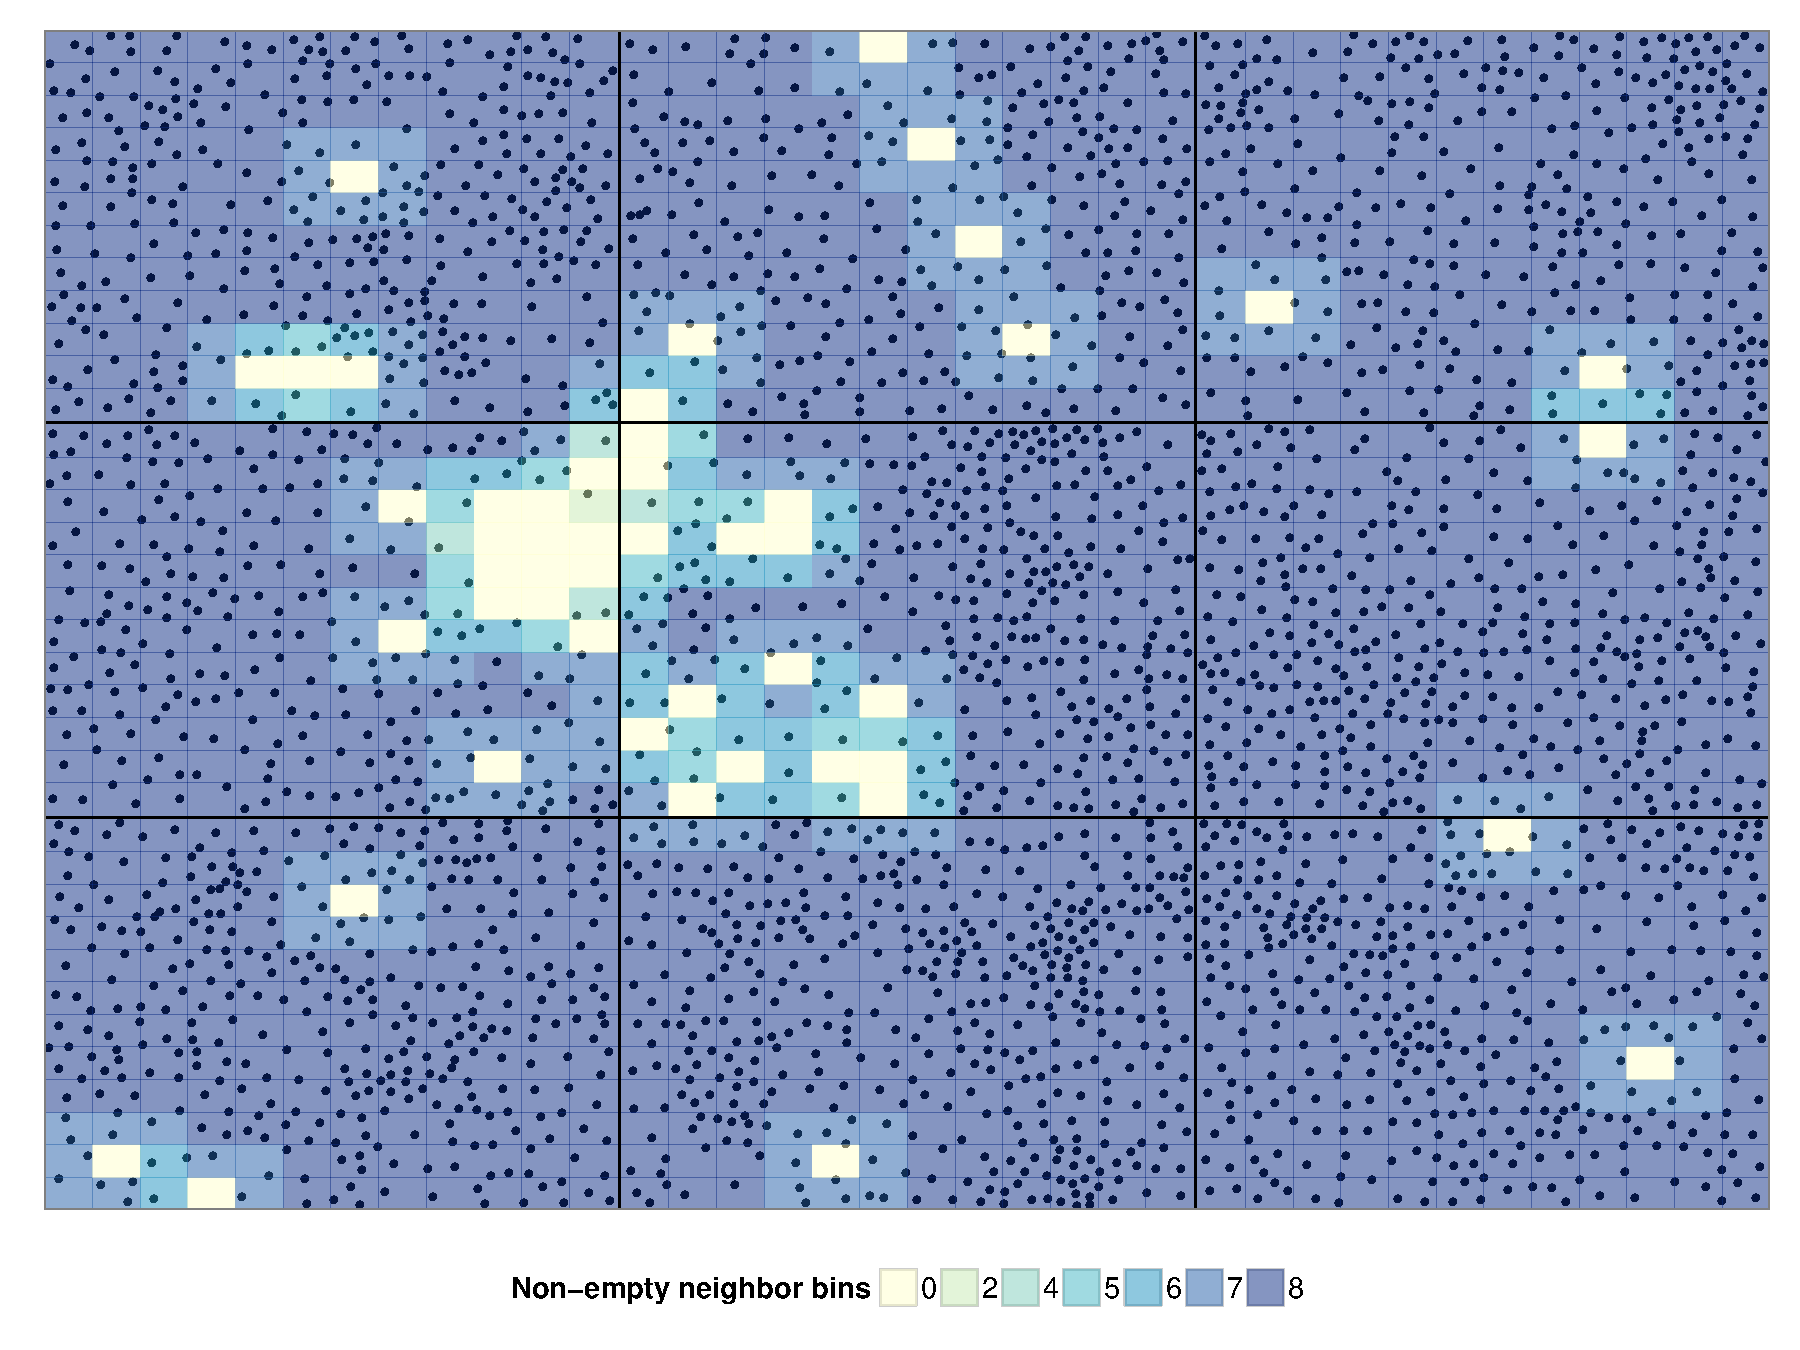
\includegraphics[width=\maxwidth]{figures/R/scf-intro/plot-scf-intro_plot-1} \caption[Visualization of cell colony edge detection by 2D binning.]{Cell colony edges are detected by 2D binning of cell center locations. Dots represent cell centers within the well H6 of plate J107-2C. Each of the nine images is segmented into 12 horizontal and 12 vertical sections yielding 144 tiles (1296 bins for the entire well). The tiles are colored according to the number of non-empty neighboring bins.}\label{fig:scf-intro_plot}
\end{figure}


\end{knitrout}


\label{ex:efficiency}
As proposed by \cite{Knapp2011} and \cite{Snijder2012}, the population context of each cell may significantly influence some morphological properties, as well as confound phenotypic information that is measured during feature extraction and therefore has to be accounted for. They propose several features that may act as proxies to characterize aspects of population context, one of which is whether a cell is located towards the border of a colony or is surrounded by cells in all directions. In order to approximate this information from location data, images are divided into 2-dimensional bins or facets and the number of cells per bin is counted. Cells that are located adjacent to one or more bins that are empty are considered edge cells and cells surrounded by non-empty bins are center cells. Figure \ref{fig:scf-intro_plot} visualizes the concept by color-coding facets according to the number of non-empty neighbors.

\begin{rlisting}{float=p}{Calculation of population context features as implemented by \citeauthor{Knapp2011}.}{In order to detect whether a cell is located towards the border of a colony or is surrounded by neighboring cells, each well is divided into 2-dimensional bins and the number of cells per bin is counted. As implemented by \citeauthor{Knapp2011}, all bins are iterated, each of the 8 possible directions (2 vertical, 2 horizontal and 4 diagonal) is checked for an empty neighbor and the corresponding binary value (at least one neighbor is empty) is saved to the current group of cells.}{edgepos}
\begin{knitrout}\footnotesize
\definecolor{shadecolor}{rgb}{0.969, 0.969, 0.969}\color{fgcolor}\begin{kframe}
\begin{alltt}
\hlstd{edgepos} \hlkwb{<-} \hlkwa{function}\hlstd{(}\hlkwc{x}\hlstd{,} \hlkwc{y}\hlstd{,} \hlkwc{img}\hlstd{,} \hlkwc{n}\hlstd{) \{}
  \hlstd{empty} \hlkwb{<-} \hlkwd{logical}\hlstd{()}
  \hlstd{xst} \hlkwb{<-} \hlstd{img[}\hlnum{1}\hlstd{]} \hlopt{/} \hlstd{n}
  \hlstd{yst} \hlkwb{<-} \hlstd{img[}\hlnum{2}\hlstd{]} \hlopt{/} \hlstd{n}
  \hlstd{sgrid} \hlkwb{<-} \hlkwd{matrix}\hlstd{(}\hlnum{0}\hlstd{,} \hlkwc{nrow}\hlstd{=n,} \hlkwc{ncol}\hlstd{=n)}
  \hlkwa{for} \hlstd{(i} \hlkwa{in} \hlnum{1}\hlopt{:}\hlstd{n) \{}
    \hlkwa{for} \hlstd{(j} \hlkwa{in} \hlnum{1}\hlopt{:}\hlstd{n) \{}
      \hlstd{ispos} \hlkwb{<-} \hlstd{(x} \hlopt{>} \hlstd{(i} \hlopt{-} \hlnum{1}\hlstd{)} \hlopt{*} \hlstd{xst)} \hlopt{&} \hlstd{(x} \hlopt{<=} \hlstd{(i} \hlopt{*} \hlstd{xst))} \hlopt{&}
               \hlstd{(y} \hlopt{>} \hlstd{(j} \hlopt{-} \hlnum{1}\hlstd{)} \hlopt{*} \hlstd{yst)} \hlopt{&} \hlstd{(y} \hlopt{<=} \hlstd{(j} \hlopt{*} \hlstd{yst))}
      \hlstd{sgrid[i, j]} \hlkwb{<-} \hlkwd{sum}\hlstd{(ispos)}
    \hlstd{\}}
  \hlstd{\}}

  \hlkwa{for} \hlstd{(i} \hlkwa{in} \hlnum{1}\hlopt{:}\hlstd{n) \{}
    \hlkwa{for} \hlstd{(j} \hlkwa{in} \hlnum{1}\hlopt{:}\hlstd{n) \{}
      \hlstd{ispos} \hlkwb{<-} \hlstd{(x} \hlopt{>} \hlstd{(i} \hlopt{-} \hlnum{1}\hlstd{)} \hlopt{*} \hlstd{xst)} \hlopt{&} \hlstd{(x} \hlopt{<=} \hlstd{(i} \hlopt{*} \hlstd{xst))} \hlopt{&}
               \hlstd{(y} \hlopt{>} \hlstd{(j} \hlopt{-} \hlnum{1}\hlstd{)} \hlopt{*} \hlstd{yst)} \hlopt{&} \hlstd{(y} \hlopt{<=} \hlstd{(j} \hlopt{*} \hlstd{yst))}
      \hlstd{isempty} \hlkwb{<-} \hlstd{F}
      \hlkwa{if} \hlstd{((i} \hlopt{>} \hlnum{1}\hlstd{)} \hlopt{&&} \hlstd{(j} \hlopt{>} \hlnum{1}\hlstd{)} \hlopt{&&} \hlstd{(sgrid[i} \hlopt{-} \hlnum{1}\hlstd{, j} \hlopt{-} \hlnum{1}\hlstd{]} \hlopt{==} \hlnum{0}\hlstd{))}
        \hlstd{isempty} \hlkwb{<-} \hlstd{T}
      \hlkwa{else if} \hlstd{((i} \hlopt{>} \hlnum{1}\hlstd{)} \hlopt{&&} \hlstd{(sgrid[i} \hlopt{-} \hlnum{1}\hlstd{, j]} \hlopt{==} \hlnum{0}\hlstd{))}
        \hlstd{isempty} \hlkwb{<-} \hlstd{T}
      \hlkwa{else if} \hlstd{((i} \hlopt{>} \hlnum{1}\hlstd{)} \hlopt{&&} \hlstd{(j} \hlopt{<} \hlstd{n)} \hlopt{&&} \hlstd{(sgrid[i} \hlopt{-} \hlnum{1}\hlstd{, j} \hlopt{+} \hlnum{1}\hlstd{]} \hlopt{==} \hlnum{0}\hlstd{))}
        \hlstd{isempty} \hlkwb{<-} \hlstd{T}
      \hlkwa{else if} \hlstd{((j} \hlopt{>} \hlnum{1}\hlstd{)} \hlopt{&&} \hlstd{(sgrid[i, j} \hlopt{-} \hlnum{1}\hlstd{]} \hlopt{==} \hlnum{0}\hlstd{))}
        \hlstd{isempty} \hlkwb{<-} \hlstd{T}
      \hlkwa{else if} \hlstd{((j} \hlopt{<} \hlstd{n)} \hlopt{&&} \hlstd{(sgrid[i, j} \hlopt{+} \hlnum{1}\hlstd{]} \hlopt{==} \hlnum{0}\hlstd{))}
        \hlstd{isempty} \hlkwb{<-} \hlstd{T}
      \hlkwa{else if} \hlstd{((i} \hlopt{<} \hlstd{n)} \hlopt{&&} \hlstd{(j} \hlopt{>} \hlnum{1}\hlstd{)} \hlopt{&&} \hlstd{(sgrid[i} \hlopt{+} \hlnum{1}\hlstd{, j} \hlopt{-} \hlnum{1}\hlstd{]} \hlopt{==} \hlnum{0}\hlstd{))}
        \hlstd{isempty} \hlkwb{<-} \hlstd{T}
      \hlkwa{else if} \hlstd{((i} \hlopt{<} \hlstd{n)} \hlopt{&&} \hlstd{(sgrid[i} \hlopt{+} \hlnum{1}\hlstd{, j]} \hlopt{==} \hlnum{0}\hlstd{))}
        \hlstd{isempty} \hlkwb{<-} \hlstd{T}
      \hlkwa{else if} \hlstd{((i} \hlopt{<} \hlstd{n)} \hlopt{&&} \hlstd{(j} \hlopt{<} \hlstd{n)} \hlopt{&&} \hlstd{(sgrid[i} \hlopt{+} \hlnum{1}\hlstd{, j} \hlopt{+} \hlnum{1}\hlstd{]} \hlopt{==} \hlnum{0}\hlstd{))}
        \hlstd{isempty} \hlkwb{<-} \hlstd{T}
      \hlstd{empty[ispos]} \hlkwb{<-} \hlstd{isempty}
    \hlstd{\}}
  \hlstd{\}}
  \hlkwd{return}\hlstd{(empty)}
\hlstd{\}}
\end{alltt}
\end{kframe}
\end{knitrout}

\end{rlisting}

Code listing \ref{lst:edgepos} constitutes an adaption of the implementation developed by \citeauthor{Knapp2011}, which is kindly provided as supplement to their publication. While iterating over all facets, only exploiting vectorization within facets and heavily relying on if-else logic, might be feasible when using datasets of the size the authors provide as demonstration material, combined with permanently storing the results, such an approach is impractical with datasets as produced by InfectX. Still, even for their datasets, the authors warn that:

\begin{quote}
These [population context feature] computations require considerable amounts of memory, and will take some time. This must be done for each of the input files, and will produce an output file containing the input data plus computed population features.
\end{quote}

\begin{rlisting}{float=p}{A more efficient implementation of calculating population context features, developed for singleCellFeatures.}{Due to the larger number of cells per well and the increase in image resolution as compared to data used in \cite{Knapp2011}, calculation of border/center population context features have to be carried out in a more efficient manner, which can be accomplished by fully vectorizing the problem.}{facetBorder}


\begin{rcode}
facetBorder <- function(x, y, img, facet) {
  facet.size <- img / facet
  # calculate facets (2d binning)
  x.bin <- ceiling(x / facet.size[1])
  y.bin <- ceiling(y / facet.size[2])
  # initialize empty grid/border matrices
  grid <- matrix(0, facet[2], facet[1])
  # calculate col-major grid index for each object
  index <- y.bin + (x.bin - 1) * facet[2]
  # summarize as counts
  counts <- table(index)
  # fill grid with counts
  grid[as.numeric(names(counts))] <- counts
  grid.res <- grid
  grid <- grid > 0
  # extend grid with a frame of ones
  grid.ext <- rbind(rep(1, (facet[1] + 2)),
                    cbind(rep(1, facet[2]), grid, rep(1, facet[2])),
                    rep(1, (facet[1] + 2)))
  # set up stencil
  row <- rep(rep(1:facet[2], facet[1]))
  col <- rep(1:facet[1], each=facet[2])
  colP1 <- col + 1
  colM1 <- col - 1
  rowP1 <- row + 1
  rowP2 <- row + 2
  nrowP <- facet[2] + 2
  stencil <- cbind(row   + colM1 * nrowP, # northwest neighbor
                   row   + col   * nrowP, # north neighbor
                   row   + colP1 * nrowP, # northeast neighbor
                   rowP1 + colP1 * nrowP, # west neighbor
                   rowP2 + colP1 * nrowP, # east neighbor
                   rowP2 + col   * nrowP, # southwest neighbor
                   rowP2 + colM1 * nrowP, # south neighbor
                   rowP1 + colM1 * nrowP) # southeast neighbor
  # apply stencil row-wise to grid
  border <- apply(stencil, 1, function(ind, mat) {
    return(sum(mat[ind]))
  }, as.numeric(grid.ext))
  # map col-major object index to border array
  return(border[index])
}
\end{rcode}


\end{rlisting}



\newcommand{\knitrScfRnaicellTotal}{\SI{2899.83}{\second}}
\newcommand{\knitrScfRnaicellEdgepos}{\SI{2892.67}{\second}}
\newcommand{\knitrScfRnaicellPercentage}{99.8\%}
\newcommand{\knitrScfRnaicellCellnoMean}{464}
\newcommand{\knitrScfRnaicellCellnoSd}{168}

An execution of the code, using the supplied exemplary dataset (number of cells per well: $\mu=\knitrScfRnaicellCellnoMean$, $\sigma=\knitrScfRnaicellCellnoSd$; 15 bins in x-direction and 15 bins in y-direction) reveals that of the \knitrScfRnaicellTotal\ spent on calculating population context features, \knitrScfRnaicellEdgepos\ (\knitrScfRnaicellPercentage\ of the total time) is spent on determining positions within colonies. This performance can be expected to deteriorate significantly, using InfectX data, due to a ten-fold increase in cell counts and more importantly a 3-fold rise in resolution in both x- and y direction. The surge in dataset size entails an increase in number of bins needed, to obtain sensible results (the example in figure \ref{fig:scf-intro_plot} is divided into 36 bins per dimension) and runtime scales as $\mathcal{O}(n^2)$ in number of bins per dimension.

Neither the high computational cost, and consequently not even storing the results, however are necessities, as demonstrated by a slightly optimized implementation (see listing \ref{lst:facetBorder}). Fully vectorizing the problem no longer requires the extensive use of if-else logic and due to R being an interpreted language, built for operating on vectors, such an approach can be expected to bring about compelling speed improvements. Vectorization is achieved by calculating the indices of the 8 neighboring bins for each facet and applying this stencil to the 2-dimensional matrix containing binary empty/non-empty information per bin. This efficiently yields the number of empty neighbors for each facet which then can be mapped to cells by their column-major grid indices. An additional advantage of the presented implementation is that the number of empty neighbors is obtained for free whereas the code proposed by \citeauthor{Knapp2011} would perform even worse if modified to produce this supplementary information, as the full set of if-statements has to be run to the end for each facet.



\newcommand{\knitrScfBenchmarkFacetMean}{\SI{7.77}{\milli\second}}
\newcommand{\knitrScfBenchmarkFacetSd}{\SI{2.69}{\milli\second}}
\newcommand{\knitrScfBenchmarkFacetTotal}{\SI{2.98} s}
\newcommand{\knitrScfBenchmarkEdgeMean}{\SI{515.85}{\milli\second}}
\newcommand{\knitrScfBenchmarkEdgeSd}{\SI{14.66}{\milli\second}}
\newcommand{\knitrScfBenchmarkEdgeTotal}{\SI{198.08}{\second}}
\newcommand{\knitrScfBenchmarkSpeedup}{66}

Benchmarking the two implementations reveals that a \knitrScfBenchmarkSpeedup -fold speedup is easily achievable only by completely vectorizing the problem. While the original code takes \knitrScfBenchmarkEdgeTotal\ per plate (384 iterations of the same well; $\mu=\knitrScfBenchmarkEdgeMean$, $\sigma=\knitrScfBenchmarkEdgeSd$; well H6 of plate J107-2C), total runtime is reduced to \knitrScfBenchmarkFacetTotal\ ($\mu=\knitrScfBenchmarkFacetMean$, $\sigma=\knitrScfBenchmarkFacetSd$, per well).

Such time-savings might not look that significant at first sight. But within the context of the available data, consequences of critical optimizations are of great value. First of all, interactive data analysis is sensitive to waiting times that exceed a few minutes and due to there not only being a single location feature to be analyzed, but rather 5--10, several minutes per feature are impractical. Moreover, if run-times can be sufficiently reduced, this makes it possible to run calculations on the fly instead of constantly saving results. Apart from the obvious downsides arising from storage overhead, management of result caches leads to practical issues whenever the workflow is under development and thus subject to constant change. Caches have to be invalidated and recomputed and the system overseeing these processes has to be made aware of changes, as well as understand where they apply.\footnote{On an anectotal note, Philip Karlton, a software engineer and former Netscape executive is quoted as saying: ``There are only two hard things in Computer Science: cache invalidation and naming things,'' corroborating the claim that it is desirable to avoid caching altogether whenever possible.} Furthermore, updating batches of data at once incurs substantial cost which might even be expended in vain if not all data is used before the next update triggers recomputation. Just in time generation of derived features is preferable over ahead of time calculation and the benefits clearly justify some optimization efforts.



\newcommand{\knitrScfFullPlateNSamp}{10}
\newcommand{\knitrScfFullPlateSampWell}{A1, A6, B1, B23, B9, E11, E14, I4, N20, P2}
\newcommand{\knitrScfFullPlateMyTime}{\SI{8.04}{\second}}
\newcommand{\knitrScfFullPlateRnaicellTime}{\SI{41.14}{\hour}}

When looking at runtimes of the original implementation obtained for benchmarking (\knitrScfBenchmarkEdgeTotal) and for a single execution on the supplied exemplary dataset (\knitrScfRnaicellEdgepos) side by side, a large discrepancy stands out. The two values are not directly comparable, as they are created with individual binning and differently sized datasets. But instead of explaining the divergence, these factors separate the two values even further, as the benchmarked time was obtained using a dataset roughly ten times larger and taking into account 6-fold more bins (225 versus 1296). Running the code of \citeauthor{Knapp2011} with InfectX data, as to be expected, takes significantly longer and determining cell position within colony for a single location feature over an entire plate is estimated to run for \knitrScfFullPlateRnaicellTime.\footnote{Due to the long running time, not all wells are processed, but \knitrScfFullPlateNSamp\ wells are randomly sampled and the mean per well is extrapolated to the full plate. The used wells are \knitrScfFullPlateSampWell\ of plate J107-2C. Moreover, it has to be emphasized once again, that the reported time-span corresponds only to the calculation of a single location feature, several of which are typically available.} The exact same results can be computed within \knitrScfFullPlateMyTime\ by the code integrated in singleCellFeatures through vectorization as discussed previously and by splitting the data into wells.

Listing \ref{lst:edgepos} does not entirely reproduce the code of \citeauthor{Knapp2011}, but constitutes a simplified version intended for highlighting the importance of vectorization and is adapted for comparison with the optimized variant. Originally, the nested for-loops iterating the bins (lines 6--12 and 14--37), are enclosed by an additional for-loop, iterating the wells. Data is stored as a large \mintinline{text}{data.frame} and all operations are performed on full-length vectors. The enormous number of comparisons resulting from this setup leads to serious performance issues, which are amplified when increasing the number of cells from $\sim 180000$ to $\sim 10^6$ per plate. Such observations, along with other considerations lead to development of a more sophisticated data structure for storing single cell feature data (see section \ref{sec:s3-objects}), which splits the data into smaller units and consequently eliminates constant comparisons against well indices for per-well operations.

The following sections discuss some design aspects and implementation issues of singleCellFeatures, beginning with data structures developed for representing single cell feature data, continuing with how data is acquired and locally cached, management of metadata and concluding with some tools for manipulating datasets as well as providing the data to third-party tools. This architectural overview is complemented by a more practical section in appendix \ref{ch:scf-manual}. For all coding, the style guide outlined in \cite{Wickham2014} was followed and \cite{Wickham2015} served as an invaluable reference, along with the extensive documentation supplied by \cite{RCoreTeam2015}. Package documentation is in-source with \mintinline{text}{.Rd} files generated by roxygen2 \citep{Wickham2015a}, which are accessible from within the R help system upon installation of the package.

\section{S3 Classes}
\label{sec:s3-objects}
\Gls{oop} in R can be achieved by any one of the three distinct object systems S3, S4 and \glspl{rc}. While the RC system resembles the \gls{oop} style most people coming from languages such as Java or C++ are familiar with, by implementing message-passing, some features such as mutability (in-place modification of objects) and pass-by-reference semantics violate common expectations of R users. S3 and S4 objects are built on the concept of generic function \gls{oop}, which does not associate methods with classes, but employs a special type of function, called a generic function, that is responsible for method dispatch. Of the two, S3 classes are more loosely organized, lacking the formal definitions of the S4 system which can describe both representation and (multiple) inheritance. Furthermore, S4 objects are capable of multiple dispatch and all code used for creating and manipulating S4 objects is not part of base R but supplied by the methods package, which introduces the new \mintinline{text}{@} operator, for accessing object slots.

Much base functionality in R is implemented using S3 classes, including lm and glm objects, the support for which has been available to R from its very beginning. The methods package for S4 objects is attached by default since version 1.7.0, but fewer packages make use of the newer syntax, some examples being the base package stats4 and CRAN packages Matrix and lme4. Bioconductor packages on the other hand are frequently designed on top of S4 classes. \Gls{rc} was only introduced with R 2.12 as part of the methods package and therefore currently does not enjoy widespread adoption. The limitations of S3 were found to be unproblematic for the planned feature set of singleCellFeatures and due to the attractive simplicity of this scheme, several objects are implemented as S3 classes.

\subsection{Metadata Objects}


\newcommand{\knitrScfMetadatNumCol}{44}
\newcommand{\knitrScfMetadatPlateQualityStat}{\mintinline{text}{UNKNOWN}, \mintinline{text}{GOOD}, \mintinline{text}{BAD} and \mintinline{text}{WARNING}}
\newcommand{\knitrScfMetadatPlateQualityFrac}{87\%}
\newcommand{\knitrScfMetadatPlateTypes}{\mintinline{text}{ScreeningPlate}, \mintinline{text}{CheckerBoard} and \mintinline{text}{MockPlate}}
\newcommand{\knitrScfMetadatSpaces}{\mintinline{text}{INFECTX} and \mintinline{text}{INFECTX_PUBLISHED}}
\newcommand{\knitrScfMetadatGeneset}{\mintinline{text}{Drug}, \mintinline{text}{Validation}, \mintinline{text}{MicroRNAome}, \mintinline{text}{Genome} and \mintinline{text}{Kinome}}
\newcommand{\knitrScfMetadatLibrary}{\mintinline{text}{Selleck}, \mintinline{text}{Ambion}, \mintinline{text}{Sigma}, \mintinline{text}{Dharmacon} and \mintinline{text}{Qiagen}}
\newcommand{\knitrScfMetadatWellQualityStat}{\mintinline{text}{UNKNOWN}, \mintinline{text}{WARNING} and \mintinline{text}{BAD}}
\newcommand{\knitrScfMetadatWellQualityFrac}{92\%}

\label{sec:metadata-objects}
Metadata is extracted from aggregate files (see section \ref{sec:aggregate-files}) and used to generate both plate-level and well-level metadata objects. These consist of key-value pairs stored as lists and accompany all plate-level and well-level data objects generated by singleCellFeatures. The R class attribute names are \mintinline{text}{PlateMeta data} or \mintinline{text}{WellMetadata} and both are associated with a superordinate object name \mintinline{text}{Metadata} in order to simplify method dispatch in cases where a function is able to operate on both object types. Table \ref{tab:plate-metadata} shows the 12 slots along with short descriptions that constitute a \mintinline{text}{PlateMetadata} object, while table \ref{tab:well-metadata} does the same for objects of type \mintinline{text}{WellMetadata} (20 key-value pairs in total). Several slots, namely \mintinline{text}{plate.barcode}, \mintinline{text}{plate.quality}, \mintinline{text}{experiment.name}, \mintinline{text}{experiment.pathogen}, \mintinline{text}{experiment.geneset} and \mintinline{text}{experiment.library}, are redundant and therefore only listed in table \ref{tab:plate-metadata}.

\renewcommand{\arraystretch}{1.5}
\setlength{\tabcolsep}{0.2em}
\begin{table}
  \centering
  \caption[Key-value pairs constituting the \mintinline{text}{PlateMetadata} structure.]{\mintinline{text}{PlateMetadata} structures consist of 12 key-value pairs intended to capture all relevant plate-wide metadata.}
  \label{tab:plate-metadata}
  \footnotesize
  \begin{tabular}{L{0.25\linewidth}L{0.7\linewidth}}
    Key name &
      Description \\
    \hline 
    \mintinline{text}{plate.barcode} &
      The unique identifier assigned to every plate, for example \mintinline{text}{KB02-1L}. \\
    \mintinline{text}{plate.quality} &
      Plate quality descriptors are \knitrScfMetadatPlateQualityStat, but currently most (\knitrScfMetadatPlateQualityFrac) are assigned the label \mintinline{text}{UNKNOWN}. \\
    \mintinline{text}{plate.type} &
      Possible values for plate type are \knitrScfMetadatPlateTypes\ and different types are characterized by their control layout. \\
    \mintinline{text}{experiment.space} &
      The first hierarchy level of data organization in openBIS. Current spaces are \knitrScfMetadatSpaces \\
    \mintinline{text}{experiment.group} &
      The group level is used to sort data according to pathogen (e.g. \mintinline{text}{ADENO_TEAM}). \\
    \mintinline{text}{experiment.name} &
      At the experiment level, data is grouped into screens. An example value is \mintinline{text}{ADENO-DP-K1}. \\
    \mintinline{text}{experiment.pathogen} &
      While the pathogen is already encoded in the openBIS hierarchy of InfectX, this is not necessarily so. In case of a different setup, the treatment applied to the screen can be saved separately. \\
    \mintinline{text}{experiment.geneset} &
      Different sets of genes are investigated throughout all screens and possible values are \knitrScfMetadatGeneset. \\
    \mintinline{text}{experiment.replicate} &
      Designates the replicate number of the current plate (see table \ref{tab:infectx-replicates}). \\
    \mintinline{text}{experiment.library} &
      Manufacturers that provide \gls{sirna} reagents to InfectX are \knitrScfMetadatLibrary. \\
    \mintinline{text}{experiment.batch} &
      Alphanumeric identifier for the batch in which the current plate was put through the wet-lab procedure. \\
    \mintinline{text}{counts.quantiles} &
      The lower and upper 5\% quantiles for cell counts over all 3456 images of the plate, determined in order to detect bad wells. \\
    \hline 
  \end{tabular}
\end{table}

\begin{table}
  \centering
  \caption[Metadata key-value pairs that make up \mintinline{text}{WellMetadata} objects.]{Analogously to \mintinline{text}{PlateMetadata} objects, \mintinline{text}{WellMetadata} classes consist of several key-value pairs. All slots that appear in both \mintinline{text}{Metadata} definitions (\mintinline{text}{plate.barcode}, \mintinline{text}{plate.quality}, \mintinline{text}{experiment.name}, \mintinline{text}{experiment.pathogen}, \mintinline{text}{experiment.geneset} and \mintinline{text}{experiment.library}) are excluded from this overview. Please refer to table \ref{tab:plate-metadata} for more information.}
  \label{tab:well-metadata}
  \footnotesize
  \begin{tabular}{L{0.25\linewidth}L{0.7\linewidth}}
    Key name &
      Description \\
    \hline 
    \mintinline{text}{well.row} &
      Capitalized alphabetic index of the current well row ($\in \{ A, B, \dotsc, P \}$). \\
    \mintinline{text}{well.col} &
      Integer-valued column index of the current well ($\in \{ 1, 2, \dotsc, 24 \}$). \\
    \mintinline{text}{well.index} &
      Well indices are calculated from row and column location and represent linearized, row-major well positions within plates ($\in \{ 1, 2, \allowbreak\dotsc, 384 \}$). \\
    \mintinline{text}{well.type} &
      Descriptor for the type of well, the most important of which include \mintinline{text}{SIRNA}, \mintinline{text}{POOLED_SIRNA} and \mintinline{text}{CONTROL}. \\
    \mintinline{text}{well.quality} &
     Possible values for this field are \knitrScfMetadatWellQualityStat, while most wells currently are set to \mintinline{text}{UNKNOWN} (\knitrScfMetadatWellQualityFrac). \\
    \mintinline{text}{gene.name} &
      Gene symbol corresponding to the targeted gene \citep{Gray2013}. \\
    \mintinline{text}{gene.id} &
      Entrez Gene ID of the targeted gene \citep{Maglott2011}. \\
    \mintinline{text}{sirna.name} &
      The \gls{sirna} catalog ID as specified by the manufacturer. \\
    \mintinline{text}{sirna.sequence} &
      Full sequence of the 5'-3' \gls{sirna} antisense (guide) strand added to the current well. \\
    \mintinline{text}{sirna.seed} &
      The seed sequence (nucleotides 2--9 from the 5' end) of the 5'-3' \gls{sirna} guide strand. \\
    \mintinline{text}{sirna.target} &
      Sense sequence of the \gls{sirna} target. \\
    \mintinline{text}{counts.cells} &
      The cell count of the current well. \\
    \mintinline{text}{counts.pathogen} &
      Count of recognized pathogen objects (in \textit{Bartonella} screens, the number of invasomes). \\
    \mintinline{text}{counts.infection} &
      Number of infected cells according to \gls{dtis}. \\
    \hline 
  \end{tabular}
\end{table}

Having metadata structures available alongside the objects holding single cell features facilitates manipulation of the data as all relevant information is bundled and does not have to be managed separately by the user. Furthermore, information stored in \mintinline{text}{well.type} can be used for normalization (sometimes it is desirable to only normalize non-control wells) and fields like \mintinline{text}{gene.name}, \mintinline{text}{gene.id} or \mintinline{text}{sirna.name} are used often for selecting the desired subset of data. The two slots \mintinline{text}{plate.quality} and especially \mintinline{text}{well.quality} hold promise for automatically discarding bad data, but current annotation levels leave much to be desired (\knitrScfMetadatPlateQualityFrac\ and \knitrScfMetadatWellQualityFrac, respectively, are labeled as \mintinline{text}{UNKNOWN}) due to the large amount of manual labor that is involved. Perhaps, if some form of automatic quality assessment is developed or if the results from focus detection are utilized to enhance data quality comments, these fields could be put to better use.

Originally, inspired by the cellHTS2 package, it was planned to use public databases for collecting further metadata, such as gene ontology, chromosomal location, gene function summaries and homology. The bioconductor package biomaRt \citep{Durinck2005,Durinck2009} can be used to query several web services, including Ensembl, Uniprot and Reactome with gene IDs \citep{Maglott2011} and retrieve gene annotations. Furthermore, \gls{sirna} sequences could be used for investigating \glspl{ote} and developing methods in order to correct for corresponding effects. Unfortunately, time constrains so far have prevented such ideas from being explored further.

\subsection{Data Objects}
Central to the presented R package are data structures that hold single cell feature data. Instead of just storing all data as a large \mintinline{text}{data.frame} as in RNAither, a more complex scheme was developed that represents the physical hierarchy of \gls{hts} datasets. This has both the advantage of presenting an intuitive structure of the data that can easily be navigated by the user, as well as efficiency benefits. Selecting cells from a well does not involve $10^6$ integer comparisons, but finding a slot in a list structure of length 384 (for consequences of the former approach, see the introductory example staring on page \pageref{ex:efficiency}).

Three types S3 objects represent the levels, data can be sorted by: 6 or 9 \mintinline{text}{ImageData} classes are assembled into a \mintinline{text}{WellData} object (which is additionally associated with a \mintinline{text}{WellMetadata} object) and 384 \mintinline{text}{WellData} structures, together with a \mintinline{text}{PlateMetadata} instance, compose a \mintinline{text}{PlateData} object. The respective collections of child objects are gathered in list structures named \mintinline{text}{data} (figure \ref{fig:scf-platedata} presents a visualization of this hierarchy). Name attributes are organized similarly as for metadata objects, with a superordinate tag \mintinline{text}{Data} assigned in addition to the individual descriptors, in order to be able to define functions that can be applied to all data objects in the same way.

The next logical level is the screen (\gls{sirna} library), but clustering several \mintinline{text}{PlateData} objects is infeasible with current hardware. As R keeps all loaded objects in memory and a plate consisting of \tilde 600 features on \tilde$10^6$ cells requires \tilde \SI{8}{\giga\byte}, only large memory systems could handle such data structures.\footnote{A large memory Euler node (a centralized \gls{hpc} resource provided by the ETH Z\"urich) was successfully used to operate on a collection of 8 \mintinline{text}{PlateData} objects for screen wide normalization trials, but the required \tilde \SI{220}{\giga\byte} of memory are currently not commonly available to desktop environments. Simply keeping the data in memory is not all that is required, as algorithmic overhead has to be factored in as well.}

\begin{figure}
  \centering
  \begin{tikzpicture}[%
    leaf/.style={grow=down,xshift=1em,anchor=west, edge from parent path={%
      (\tikzparentnode.south) |- (\tikzchildnode.west)}
    },
    level 1/.style={sibling distance=18em},
    level 2/.style={sibling distance=4em},
    level 3/.style={sibling distance=14em},
    level 4/.style={sibling distance=4em},
    vertex style/.style={
      draw=#1,
      thick,
      fill=#1!70,
      text=white,
      minimum width=1cm,
      minimum height=0.5cm,
      font=\footnotesize
    }
  ]
    \node[vertex style=Turquoise]{PlateData}
    [edge from parent fork down]
    child{node[vertex style=SeaGreen] {PlateMetadata}
      child[leaf,level distance=6ex] {%
        node[vertex style=BurntOrange]{plate.barcode}}
      child[leaf,level distance=12ex] {%
        node[vertex style=BurntOrange]{plate.quality}}
      child[leaf,level distance=18ex] {%
        node[vertex style=BurntOrange] {plate.type}}
      child[leaf,level distance=24ex] {%
        node[vertex style=BurntOrange] {\ldots}}
      child[leaf,level distance=30ex] {%
        node[vertex style=BurntOrange] {experiment.library}}
    }
    child {node[vertex style=MidnightBlue] {data}
      child {node[vertex style=Turquoise] {A1}}
      child {node[vertex style=Turquoise] {A2}
        child {node[vertex style=SeaGreen] {WellMetadata}
          child[leaf,level distance=6ex] {%
            node[vertex style=BurntOrange]{well.index}}
          child[leaf,level distance=12ex] {%
            node[vertex style=BurntOrange]{well.type}}
          child[leaf,level distance=18ex] {%
            node[vertex style=BurntOrange] {gene.name}}
          child[leaf,level distance=24ex] {%
            node[vertex style=BurntOrange] {\ldots}}
          child[leaf,level distance=30ex] {%
            node[vertex style=BurntOrange] {sirna.sequence}}
        }
        child {node[vertex style=MidnightBlue] {data}
          child {node[vertex style=Turquoise] {img\_11}
            child[leaf,level distance=6ex] {%
              node[vertex style=BurntOrange]{image.index}}
            child[leaf,level distance=12ex] {%
              node[vertex style=BurntOrange]{\ldots}}
            child[leaf,level distance=18ex] {%
              node[vertex style=MidnightBlue]{data.vec}}
            child[leaf,level distance=24ex] {%
              node[vertex style=MidnightBlue]{data.mat}}
            child[leaf,level distance=30ex] {%
              node[vertex style=MidnightBlue] {data.lst}}
          }
          child {node[vertex style=Turquoise] {img\_12}}
          child {node[vertex style=Turquoise] {\ldots}}
          child {node[vertex style=Turquoise] {img\_33}}
        }
      }
      child {node[vertex style=Turquoise] {\ldots}}
      child {node[vertex style=Turquoise] {P24}}
    };
  \end{tikzpicture}
  \caption[Data structure used for representing a complete plate of single cell data.]{Single cell data is organized according to the hierarchy imposed by \gls{hts} experiment design. Plates are divided into wells which are subdivided into images and Metadata objects (green) are attached at each level. Data objects provided by singleCellFeatures are in light blue and contain lists of subordinate objects (dark blue), while Metadata objects consist of key-value pairs (orange).}
  \label{fig:scf-platedata}
\end{figure}

The slots of \mintinline{text}{ImageData} objects are \mintinline{text}{plate} (barcode), \mintinline{text}{well.index} (linear, row-major, $\in \{ 1, 2, \dotsc, 384 \}$), \mintinline{text}{well.row} ($\in \{ A, B, \dotsc, P \}$), \mintinline{text}{well.col} ($\in \{ 1, 2, \dotsc, 24 \}$), \mintinline{text}{image.index} (linear, row-major, $\in \{ 1, 2, \dotsc, 6 \} \lor \{ 1, 2, \dotsc, 9 \}$, depending on number of imaging sites), \mintinline{text}{image.row} ($\in \{ 1, 2 \} \lor \{ 1, 2, 3 \}$, for 6 and 9 image wells, respectively), \mintinline{text}{image.col} ($\in \{ 1, 2, 3 \}$, independent on total number of images), \mintinline{text}{image.total} ($\in \{ 6, 9 \}$), \mintinline{text}{counts.quantiles} (the lower and upper 5\% quantiles of plate-wide, image level cell counts), \mintinline{text}{counts.cells}, \mintinline{text}{data.vec}, \mintinline{text}{data.mat} and \mintinline{text}{data.lst}.

Actual feature data is split according to dimensionality with respect to images or detected objects within images. Scalar-valued entities (such as object counts, minima, maxima, etc.) are saved into \mintinline{text}{data.vec} which represents the concatenated data as a vector-valued \mintinline{text}{data.frame} (in order to accommodate both numerical and character fields). Vector-valued features (the bulk of single cell data) are assembled into matrices, dependent on object counts, which are added to \mintinline{text}{data.mat}. While there are typically as many nuclei as cells, those features can be merged into the same matrix, but pathogen objects require their own data structure, as pathogen counts are different from cell counts. Furthermore, it may happen that cellular features come in different lengths due to segmentation errors. A final group of features is vector-valued per cell (matrix-valued per image) and is saved to the \mintinline{text}{data.lst} node. Currently, neighbor features are detected and converted to sparse adjacency matrices, using the Matrix package \citep{Bates2015}, while others, such as parent\slash child features, are represented by nested list structures.

One obvious advantage of the proposed data representation is storage efficiency for values that apply to groups of cells, such as plate and well-level metadata or all features of the \mintinline{text}{data.vec} group. When using a large matrix for all data, this information has to be duplicated \tilde 400 times at image level, \tilde 3500 times at well level and \tilde $10^6$ times at plate level, incurring significant storage overhead. This can be mitigated somewhat by using factors and the resulting structures can still be handled well by current hardware, but nonetheless, parsimony is desirable. For these reasons, metadata objects at image level were not developed, as they unnecessarily inflate object size, despite this breaking recursive symmetry. Instead, only the minimally necessary information for identifying the data source is attached at this level.

In retrospect, it is debatable whether spiting data into images is sensible or creates unnecessary computational overhead in traversing nested lists. At the time of original implementation it was unclear if all images could be treated equally and having this level of granularity available seemed important. With access to some practical experience in working with such structures, this feature may not be worth the complexity it entails. Splitting the data at well level, however has proven to be worthwhile.

\subsection{Auxiliary Objects}
\label{sec:auxiliary-objects}
Several additional S3 objects are implemented in an auxiliary capacity. Both \mintinline{text}{PlateLocation} and \mintinline{text}{WellLocation} classes serve to communicate the identity and location of datasets, while \mintinline{text}{PlateAggregate} and \mintinline{text}{MatData} objects are used for caching purposes.

Objects representing data locations are simple key-value lists that are instantiated with a barcode in case of \mintinline{text}{PlateLocation} or a barcode and a row\slash column specification for \mintinline{text}{WellLocation} objects. Subsequent population of slots \mintinline{text}{space}, \mintinline{text}{group} and \mintinline{text}{experiment} is performed by lookup of the information in the \mintinline{text}{plate.database} table (see section \ref{sec:plate-database}), which is an optimization measure necessary to speed up creation times severely hampered by retrieving the values from large aggregate files. The information contained in \mintinline{text}{DataLocation} (the class attribute to specify any of the two location types) objects uniquely specifies where the described dataset is located on openBIS and in local file-system cache and these classes are mainly used for unifying package-internal communication.

\begin{rlisting}{float=t}{Exemplary application of \mintinline{text}{DataLocation} objects.}{Mostly used for internal communication of dataset identity and location both within openBIS and the local file system, \mintinline{text}{DataLocation} objects simplify certain tasks such as lookup of cache files.}{getCacheFilenameData}


\begin{rcode}

getCacheFilenameData <- function(x) {
  UseMethod("getCacheFilenameData", x)
}

getCacheFilenameData.WellLocation <- function(x) {
  config <- configGet()
  name <- paste0(x$plate, "_", x$row, x$col, "_sc_all.rds")
  path <- paste(config$dataStorage$dataDir, x$space, x$group, 
    x$experiment, x$plate, "WellData", name, sep = "/")
  return(path)
}

getCacheFilenameData.PlateLocation <- function(x) {
  config <- configGet()
  name <- paste0(x$plate, "_sc_all.rds")
  path <- paste(config$dataStorage$dataDir, x$space, x$group, 
    x$experiment, x$plate, name, sep = "/")
  return(path)
}

getCacheFilenameData.default <- function(x) {
  stop("can only deal with DataLocation (PlateLocation/WellLocation) objects.")
}

\end{rcode}


\end{rlisting}

Before introduction of \mintinline{text}{DataLocation} objects, a fair amount of redundant code was necessary for simple tasks such as saving or retrieving cache files. Identity of datasets was mostly specified by passing plate barcodes\slash experiment names and from that information, paths were assembled. Cumbersome casting of letter case, splitting strings to separate pathogen from library and adding setup-specific strings (such as \mintinline{text}{_TEAM}, which added as suffix to an all caps pathogen name yields the openBIS project name) to generate the appropriate values determining local file paths, as well as performance issues due to constant lookups of the same information can altogether be avoided by using specialized objects containing all neccessary information. Furthermore, the S3 method dispatch system can be put to use for specifying different behavior dependent on the object that is used as function argument. For a small illustration of such as use case, see code listing \ref{lst:getCacheFilenameData}.

The two remaining auxiliary objects are both used for caching purposes. Due to the narrow purpose of \mintinline{text}{DataLocation} a lookup table containing all required information can be created, that remains small enough to be loaded quickly. This is not possible for creating metadata objects, as most aggregate file columns are required for this process. In order to prevent repeated loading of these large files (100--\SI{200}{\mega\byte}, plate-level excerpts are cached as \mintinline{text}{PlateAggregate} objects whenever first accessed. The resulting files are small (\tilde \SI{100}{\kilo\byte}) and can be attached quickly. The data structure is simple, containing of two slots \mintinline{text}{plate} and \mintinline{text}{data}, the former holding a \mintinline{text}{PlateLocation} object and the latter a \mintinline{text}{data.frame} storing the relevant 384 rows of the corresponding aggregate file.

Finally, \mintinline{text}{MatData} is a type of \mintinline{text}{Data} object, that can be though of as a precursor to a \mintinline{text}{PlateData} object. The reason for its existence lies in the dynamic nature of this project. Many parts of singleCellFeatures evolved considerably and constant change poses problems for cached data structures. Originally, \mintinline{text}{PlateData} objects themselves were saved to the local file system but whenever their implementation was modified, all instances had to be invalidated and rebuilt (which initially took \tilde\SI{45}{\minute} per plate). In order to improve the situation, not \mintinline{text}{PlateData} objects are written to disk, but a data structure that holds all MATLAB feature data in a large nested list, as it is imported into R. Two slots are available to a \mintinline{text}{MatData} object, one called \mintinline{text}{meta} and intended for holding a \mintinline{text}{PlateMetadata} object and the oder is named \mintinline{text}{data} and stores all single cell features.

This successfully addresses the outlined problem, since the raw data will not change frequently (it still can occur that for example new features are developed\footnote{The system is build with a fair amount of flexibility, as there are methods available for adding new features to existing \mintinline{text}{MatData} structures, including automatic invalidation of downstream well caches. Therefore, extraction of new features does not require the rebuild of whole \mintinline{text}{MatData} objects.}, or better segmentation is employed), but introduces a new issue: build up of \mintinline{text}{PlateData} objects from \mintinline{text}{MatData} has to be reasonably fast due to this being the first step in every interactive session. Some aspects of how this is achieved is discussed in section \ref{sec:data-access}.

None of these auxiliary data structures are implemented as S3 objects for simply defining a set of fields, but much rather for their capability of using generic functions that specify how a specific procedure is applied to the different object variants. While this by itself is not an indispensable feature, as one could simple choose different but related names for the set of procedures, it is greatly appreciated for helping to organize code into functional units. Furthermore, this reduces the amount of redundant code by allowing the same function name to be applied in different contexts (for examples of this, see listings \ref{lst:feature-compat} and \ref{lst:convert}).

\section{Data Access}
\label{sec:data-access}
The core capability of singleCellFeatures is seamlessly providing the user with single cell data and doing this within time-frames that are suitable for interactive usage. As already discussed in the introduction to this chapter, some form of local caching is necessary to to meet these goals, as downloading data from openBIS and especially loading a large number of MATLAB \mintinline{text}{.mat} files into R takes a considerable amount of time.

Several tools were developed, beginning with search capabilities in order to locate the datasets of interest, followed by a set of functions that sort the queried data into units such that fetching is as economical as possible thusly minimizes waiting times and trigger retrieval from a multilevel cache system. All of this is handled in the background with no user intervention required. The following short example is intended for highlighting the effectiveness of the proposed system.



\begin{rflow}
time <- system.time({
  plates <- findPlates(contents="MTOR",
                       experiments="brucella-du-k[12]")
  wells  <- findWells(contents=c("MTOR", "SCRAMBLED"),
                      plates=unlist(plates))
  data   <- getSingleCellData(wells)})
\end{rflow}

\newcommand{\knitrScfFindGetDemoTime}{\SI{44}{\second}}
\newcommand{\knitrScfFindGetDemoSize}{\SI{1.22}{\giga\byte}}
\newcommand{\knitrScfFindGetDemoLengthW}{104}
\newcommand{\knitrScfFindGetDemoLengthP}{8}


In order to retrieve data from all plates containing wells with \gls{sirna} directed against \gls{mtor}, a list of \mintinline{text}{PlateLocations} is generated by \mintinline{text}{findPlates}. Acting on that structure, \mintinline{text}{findWells} selects all wells containing scrambled control \gls{sirna}, as well as \gls{mtor} knockdown wells and returns a list of \mintinline{text}{WellLocations}. Retrieving the resulting \knitrScfFindGetDemoLengthW\ wells, spread over \knitrScfFindGetDemoLengthP\ plates (\knitrScfFindGetDemoSize\ of data), is accomplished within \knitrScfFindGetDemoTime. In this case, all well data was read from cache, but apart from an increase in runtime, the same code snippet can be used irrespective of local cache state and will produce identical results. Figuring out how to proceed most efficiently in any case is handled by singleCellFeatures.

\begin{figure}
  \centering
  \begin{tikzpicture}[%
    decision style/.style={%
      diamond, draw=#1, on grid, thick, fill=#1!70, inner sep=2pt, aspect=2, 
      text=white, text width=5em, text centered, font=\footnotesize
    },
    block style/.style={%
      rectangle, draw=#1, on grid, thick, fill=#1!70, rounded corners,
      minimum height=3em, inner sep=4pt, minimum width=7em, text=white,
      text width=5em, text centered, font=\footnotesize
    },
    cloud style/.style={%
      ellipse, draw=#1, on grid, thick, fill=#1!70, minimum height=3em,
      minimum width=6em, inner sep=2pt, text=white, text width=5em,
      text centered, font=\footnotesize
    },
    line style/.style={%
      draw, -latex'
    }
  ]
  % Place nodes
  \node [cloud style=SeaGreen] (dataLoc) {%
    List of \mintinline{text}{DataLocation} objects};
  \node [block style=SeaGreen, left = 3.75cm of dataLoc] (find) {%
    Find data (wells, plates)};
  \node [block style=Turquoise, right = 3.75cm of dataLoc] (sort) {%
    Sort \mintinline{text}{DataLocations} by plate};
  \node [decision style=Turquoise, below = 2.5cm of dataLoc] (onlyWell) {%
    Were only cached wells requested?};
  \node [cloud style=Turquoise, below = 2.5cm of find] (done) {%
    Add to results};
  \node [block style=Turquoise, below = 2.5cm of sort] (iterate) {%
    Iterate plates};
  \node [decision style=BurntOrange, below = 2.5cm of iterate] (plateCache) {%
    Does \mintinline{text}{MatData} cache exist?};
  \node [decision style=BurntOrange, below = 2.5cm of plateCache] (matFiles) {%
    Are \mintinline{text}{.mat} files present?};
  \node [block style=BurntOrange, below = 2.5cm of matFiles] (download) {%
    Download data from openBIS};
  \node [block style=BurntOrange, left = 3.75cm of matFiles] (import) {%
    Import \mintinline{text}{.mat} data into R, save
    \mintinline{text}{MatData} cache};
  \node [cloud style=BurntOrange, left = 3.75cm of plateCache] (plateData) {%
    Build \mintinline{text}{PlateData} object};
  \node [decision style=Turquoise, left = 3.75cm of plateData] (wellReq) {%
    Were any uncached wells requested?};
  \node [block style=Turquoise, left = 3.75cm of import] (wellCache) {%
    Extract wells, cache \mintinline{text}{WellData} objects};
  % Draw edges
  \path [line style] (find) -- (dataLoc);
  \path [line style] (dataLoc) -- (sort);
  \path [line style] (sort) -- (iterate);
  \path [line style] (iterate) -- (onlyWell);
  \path [line style] (done.north) |-(0cm,-1.25cm)-| (iterate.north);
  \path [line style] (onlyWell) |-(0cm,-3.75cm)-| node[pos=0.25,above]{%
    no}(plateCache);
  \path [line style] (onlyWell) -- node[above]{yes}(done);
  \path [line style] (plateCache) -- node[right]{no}(matFiles);
  \path [line style] (matFiles) -- node[right]{no}(download);
  \path [line style] (download) -| (import);
  \path [line style] (matFiles) -- node[above]{yes}(import);
  \path [line style] (plateCache) -- node[above]{yes}(plateData);
  \path [line style] (import) -- (plateData);
  \path [line style] (plateData) -- (wellReq);
  \path [line style] (wellReq) -- node[right]{no}(done);
  \path [line style] (wellReq) -- node[right]{yes}(wellCache);
  \path [line style] (wellCache.west) |-(-5.75cm,-7.5cm)|- (done.west);
  \end{tikzpicture}
  \caption[Simplified view of the steps involved in loading single cell data.]{Three separate procedures are involved in loading single cell data. First, the functions \mintinline{text}{findPlates} and \mintinline{text}{findWells} can be used to run queries and retrieve a list of \mintinline{text}{DataLocation} objects (green) which is passed on to the function \mintinline{text}{getSingleCellData} (blue). Data requests are sorted according to plate and the list of plates is iterated. Dependent on request and availability of caches, \mintinline{text}{DataLocation} objects are assembled (orange) and returned to the calling function. This diagram represents a simplified view and several additional features complicate the underlying logic. For example, only a subset of features can be requested, in which case, writing of well caches has to be handled separately. Furthermore, checks for data completeness and consistency are employed that may alter the outlined execution path and mechanisms for recovery from unsuccessful imports are also in place but not shown.}
  \label{fig:scf-data-import}
\end{figure}

The most important steps in this procedure are visualized by figure \ref{fig:scf-data-import}. For sake of brevity, several aspects that complicate the logic underlying data access are omitted from the diagram. Some examples include recovery from failed downloads or imports, checks for completeness and consistency of the fetched data, issues involving metadata and the ability to only retrieve a subset of single cell feature, which requires special attention to down-stream caching. Color coding corresponds to the functional units searching (green), ordering the query and executing individual fetches (blue), as well as building the required data structures (orange). 

Searching relies on search indexes that are stored as a single plate database and pathogen specific well databases in order to be carried out quickly and economically. These lookup tables are derived from metadata contained in aggregate files and are described in detail in sections \ref{sec:plate-database} and \ref{sec:aggregate-files}. Further information regarding search functionality, such as arguments recognized by the two functions and how exactly search strings are matched is available in section \ref{sec:dataset-search}. The resulting list of \mintinline{text}{DataLocation} objects is passed to the function \mintinline{text}{getSingleCellData}, which acts as a conduit between searches and fetches.

The inquiry has to be ordered plate wise, in case uncached wells are sought from different plates. If such requests are carried out interleaved, large plate caches are read redundantly, entailing unnecessary overhead. The plates involved are iterated and it is checked if only cached wells are requested, in which case they are read from disk and added to the result structure. If uncached wells need to be made available or a complete plate is solicited, the corresponding \mintinline{text}{PlateData} object has to be built, the particularities which (orange nodes in figure \ref{fig:scf-data-import}) will be explored throughout the following subsections. Finally, if only wells were requested, they are extracted from the \mintinline{text}{PlateData} structure and added to the list of results and if the complete plate data is of interest it is returned as-is.

Green and blue nodes in figure \ref{fig:scf-data-import} can be bypassed entirely if only few single data structures are of interest. Instantiating a single \mintinline{text}{WellData} object, for example, that is not cached, will trigger the build up of a \mintinline{text}{PlateData} structure, followed by the extraction of that well. This, of course is inefficient, if multiple wells of the same plate are needed, as the plate structure is repeatedly created and discarded. In such a scenario, the functions described above can be utilized, or \mintinline{text}{PlateData} object itself can be instantiated, following well extraction initiated by the user (via the functionality provided by \mintinline{text}{extractWells}). These concepts are best illustrated by a quick example:

\label{ex:dataobject-instantiation}
\begin{rflow}
# set up a few data location objects
well.locs <- list(WellLocation("J107-2C", "H", 6),
                  WellLocation("J107-2C", "G", 23))
# inefficient if well caches do not exist, as the corresponding plate
# cache will be loaded twice, otherwise quickest option
wells <- lapply(well.locs, WellData)
# best if plate data already loaded or well caches inexistent
plate <- PlateData(convertToPlateLocation(well.locs[[1]]))
wells <- extractWells(plate, well.locs, keep.plate=FALSE)
# singleCellFeatures figures out how to proceed optimally
wells <- getSingleCellData(well.locs)
\end{rflow}

The remainder of the current section will focus on topics revolving around data provisioning itself, involving data acquisition, caching and build-up of \mintinline{text}{PlateData} structures (orange nodes in figure \ref{fig:scf-data-import}).

\subsection{Data Download}
Fetching data from openBIS, in case neither corresponding MATLAB files, nor a \mintinline{text}{MatData} cache file exists,\footnote{A third scenario that will trigger data download is manual override. If, for some reason cached data gets corrupted, or if a newer version of a dataset is available on openBIS, the user can choose to re-download individual plates. In addition, removal of all caches can be triggered, but for most circumstances this presents too drastic a measure.} is performed by issuing a system call and running the Java command line executable that is supplied with openBIS. Currently, three different types of files can be downloaded

\begin{center}
\mintinline{text}{HCS_ANALYSIS_CELL_FEATURES_CC_MAT}
\mintinline{text}{HCS_ANALYSIS_CELL_DECTREECLASSIFIER_MAT}
\mintinline{text}{HCS_ANALYSIS_CELL_THRESHOLDEDINFECTIONSCORING_MAT}
\end{center}

and the downloading routine can be run in two different modes, one targeting single cell feature files (filtering for the first file type, \mintinline{text}{FEATURES_CC}), while the other is intended for fetching \gls{dtis} results and prefers \mintinline{text}{DECTREECLASSIFIER} but falls back to \mintinline{text}{THRESHOLDEDINFECTIONSCORING} when the former is unavailable. The two types of infection scores represent two generations of \gls{dtis} procedures (distinct from \gls{svm} based scoring which were used before) and while the newer files are available for many plates, there are some that have not yet been updated. The downloaded set of files can further be refined by supplying a regular expression that is passed on the Java utility, but this will prevent downstream caches from being created (at well level) and create a plate level cache that is incomplete (can be completed without re-fetching the already downloaded data). All \mintinline{text}{.mat} files are saved to a temporary location within the directory structure managed by singleCellFeatures.

\subsection{Data Import}
Following completion of all download tasks, the resulting list of files is read into R using the function \mintinline{text}{readMat} of R.matlab \citep{Bengtsson2015}. For unknown reasons this function sometimes fails to import a file,\footnote{Failure is rare and does not seem to be dependent on file-level corruption, as retrying the same file usually resolves the problem. Furthermore, so far, no patterns could be made out, in that affected files appear to be somewhat random. The issue was not investigated further as a pragmatic approach resolved the problem.} which is caught, the affected file is saved into a special directory and import is allowed to continue. Due to this being the most time-consuming step in data provisioning, the results are stored as incomplete \mintinline{text}{MatData} caches and functionality for completing the data structure as opposed to entirely rebuilding it, are available. The function \mintinline{text}{rebuildCache} automatically retries files that failed during initial import and is capable of re-downloading individual features from openBIS that are missing from the \mintinline{text}{MatData} structure without user intervention.\footnote{The necessity for re-downloading is distinct from re-importing. While the latter arises from the possibility of failed reads of \mintinline{text}{.mat} files, the former is a consequence of problems that surround the openBIS hardware implementation of InfectX. Due to infrastructure work during much of the time of this project, it could not be guaranteed that the downloaded set of features comprises the full set of available features. This issue is remedied by checking for completeness of the local feature-set after build-up of a \mintinline{text}{MatData} structure in combination with semi-autonomous and cheap addition of individual features in case some are found to be missing.}\footnote{\label{fn:feat-check}Missingness currently is determined by comparison to a pathogen specific list of features. While being a very simple approach, it may lead to false positives (features that are indicated to be missing but do not exist), as well as false negatives (features that are present but indicated to be superfluous), as the set of features is not only pathogen specific, but also dependent on the analysis pipeline version. Improvements to this scheme are feasible (for example querying openBIS metadata directly or creating screen level lists) but not implemented due to time constraints and acceptable performance of the current system (see section \ref{sec:feature-lists} for more information).} Furthermore, the location of manually downloaded files can be specified in order for them to be added to the data structure and down stream caches of \mintinline{text}{WellData} structures are automatically removed whenever the \mintinline{text}{MatData} object is rewritten, as they are no longer valid.

Upon successful assembly of a \mintinline{text}{MatData} object, it is written to disk. Due to the large size of these objects (a typical plate is \tilde \SI{8}{\giga\byte} in size) good and efficient compression is essential both from a perspective of economically utilizing storage space, as well as from the viewpoint of time consumption. All major compression programs (bzip2, gzip, xz and zip) offer a parameter to adjust the speed\slash file size trade-off (usually an integer between 1 and 9) but a high compression ratio entails significant performance penalties. For storage of \mintinline{text}{MatData} objects, smallest file sizes were obtained using xz with flags \mintinline{text}{-9} or \mintinline{text}{-e}, which were on the order of 1--\SI{1.5}{\giga\byte}.

\begin{rlisting}{float=t}{Wrapper around pigz in order to speed up compression times for \mintinline{text}{MatData} objects.}{Compression with base library functions is not sufficiently performant, leading to the implementation of functions wrapping around \mintinline{text}{readRDS}\slash\mintinline{text}{saveRDS} that are capable of exploiting parallelized compression algorithms. The best overall compromise between compression\slash decompression speed and file size was obtained with pigz at compression level setting \mintinline{text}{-9}.}{pigz}


\begin{rcode}

saveRDSMC <- function(object, file, threads = getNumCores()) {
  message("using ", threads, " threads for compression.")
  con <- pipe(paste0("pigz -p ", threads, " -9 -f > ", file), "wb")
  saveRDS(object, file = con)
  on.exit(if (exists("con")) close(con))
}

readRDSMC <- function(file) {
  con <- pipe(paste0("pigz -d -k -c ", file))
  object <- tryCatch({
    readRDS(file = con)
  }, error = function(err) {
    stop("could not read file\n", file, ":\n", err)
  }, finally = {
    if (exists("con")) close(con)
  })
  return(object)
}

\end{rcode}


\end{rlisting}

While slightly longer compression times might be worth the savings in storage space, the time required for decompression is critical, as it will be the first step of every analysis procedure. Unfortunately, retrieval of highly compressed xz files is too slow for this application. Moreover, parallelized implementations lbzip2, p7zip, PBZIP2, pigz and xz with option \mintinline{text}{-T} were tested and and the best overall compromise is achieved using pigz with option \mintinline{text}{-9}, as shown in code listing \ref{lst:pigz}. Typical file sizes using this procedure are 1.5--\SI{2}{\giga\byte} for a complete \mintinline{text}{MatData} object and compression takes around \SI{10}{\minute}.

After the plate cache file is written, all successfully read \mintinline{text}{.mat} files are deleted, while failed files are kept for subsequently re-attempting import. Whenever the cache is read from disk, it is checked for feature completeness and the user is informed of deviations from the expected state. Due to the current implementation this is prone to some erroneous warnings especially for older plates that have not been updated to the newest feature extraction procedures (see footnote \ref{fn:feat-check}), upon which reporting is based.

\subsection{Creation of \mintinline{text}{Data} Structures}
Irrespective of whether a given plate is already in cache or is requested for the first time, every \mintinline{text}{PlateData} structure is built from a \mintinline{text}{MatData} object. As mentioned in section \ref{sec:auxiliary-objects}, the motivation behind this is creating independence between the implementation of \mintinline{text}{PlateData} structures and the data itself and consequently no longer invalidating cached plate data by making changes to its representation. This requires the conversion of \mintinline{text}{MatData} into \mintinline{text}{PlateData} to be reasonably fast and much effort was invested in reducing the amount of time needed for this step.

The critical section in this process is creating the individual \mintinline{text}{ImageData} objects from the list structure resembling how single cell features are stored by CellProfiler. Listing \ref{lst:splitImages} displays a segment of the code involved and while it might appear cluttered at first sight and the context of many variables is unclear, it is reproduced in order to highlight some important aspects. At this point in execution, among other things, the features have been sorted into groups according to their dimensions. Every feature is represented by a list containing as many slots as there are images on a plate and each slot holds a further list structure, the length of which is used for sorting. Single element objects are grouped into \mintinline{text}{vec} and handled by the code in lines 4--10, lists with multiple scalar elements are added to \mintinline{text}{mat} and treated by lines 12--29, while entries that constitute of a further nesting level are stored in \mintinline{text}{lst} and dealt with by lines 31--73. With this structure established, the outermost \mintinline{text}{apply}-type function sets up an index that moves through all lists simultaneously and in each step, the data corresponding to the given image is extracted and molded into an \mintinline{text}{ImageData} structure.

\afterpage{\clearpage\begin{rlisting}{enlarge bottom finally by=0.75cm, nofloat}{An excerpt of the code resposible for converting \mintinline{text}{MatData} into \mintinline{text}{PlateData} objects.}{Due to the heterogeneity of InfectX datasets, build up of \mintinline{text}{PlateData} structure is fairly involved, as many edge cases have to be handled. Moreover, every instantiation of a \mintinline{text}{PlateData} object is preceded by the conversion from a \mintinline{text}{MatData} structure, requiring quick turnover. This code excerpt shows the section responsible for building \mintinline{text}{ImageData} objects from a nested list structure akin to what is produced by CellProfiler, by moving through all lists simultaneously and in building an image data object in every iteration. The three sections \mintinline{text}{vec}, \mintinline{text}{mat} and \mintinline{text}{lst} correspond to different types of features that are grouped according to their dimensions.}{splitImages}
\begin{rcode}
data$data <- plyr::llply(1:tot.nimgs, function(ind, data, name,
                                               n.imgs, quants, counts) {
  if(length(data$vec) > 0) {
    vec <- lapply(data$vec, function(group, ind) {
      return(data.frame(lapply(group, function(feature, i) {
        return(feature[[i]])
      }, ind), stringsAsFactors=FALSE, check.names=FALSE, check.rows=FALSE))
    }, ind)
  } else {
    vec <- NULL
  }
  if(length(data$mat) > 0) {
    mat <- lapply(data$mat, function(group, ind) {
      n.rows <- length(group[[1]][[ind]])
      grp <- vapply(group, function(feature, i) {
        return(unlist(feature[i]))
      }, double(n.rows), ind)
      names <- colnames(grp)
      if(is.null(names)) names <- names(grp)
      n.cols <- length(names)
      dim(grp) <- c(n.rows, n.cols)
      colnames(grp) <- names
      rownames(grp) <- NULL
      return(grp)
    }, ind)
  } else {
    mat <- NULL
  }
  if(length(data$lst) > 0) {
    lst <- mapply(function(group, gname, ind) {
      if(gname == "IdentityOfNeighbors") {
        return(lapply(group, function(feature, i) {
          # build sparse adjacency matrices
          l <- length(feature[[i]])
          if(l > 1) {
            p <- c(0, cumsum(sapply(feature[[i]],
                             function(x) length(x[[1]]))))
            j <- unlist(feature[[i]])
            return(sparseMatrix(j=j, p=p, dims=c(l, l)))
          } else return(NULL)
        }, ind))
      } else if(gname == "PercentTouchingNeighbors") {
        return(lapply(group, function(feature, i) {
          if(length(feature[[i]]) > 1) return(unlist(feature[[i]]))
          else return(NULL)
        }, ind))
      } else {
        return(lapply(group, function(feature, i) return(feature[i]), ind))
      }
    }, data$lst, names(data$lst), list(ind=ind), SIMPLIFY=FALSE)
  } else {
    lst <- NULL
  }
  if(!is.null(lst$PercentTouchingNeighbors) & 
     !is.null(lst$IdentityOfNeighbors)) {
    lst$PercentTouchingNeighbors <- mapply(function(feat, fname, mats) {
      object <- unlist(strsplit(fname, 
                                "Neighbors.PercentTouchingNeighbors"))[2]
      mat <- mats[[grep(paste0("Neighbors.IdentityOfNeighbors", object),
                        names(mats))]]
      if(is.null(mat)) {
        return(feat)
      } else {
        return(sparseMatrix(j=mat@i, p=mat@p, x=feat, dims=dim(mat),
               index1=FALSE))
      }
    }, lst$PercentTouchingNeighbors, names(lst$PercentTouchingNeighbors),
       list(mats=lst$IdentityOfNeighbors), SIMPLIFY = FALSE)
  }
  return(ImageData(name, ind, n.imgs, quants, counts[ind], vec, mat, lst))
}, data$data, getBarcode(plate), n.imgs, data$meta$counts.quantiles,
cell.counts, .progress=progress.bar)
\end{rcode}
\end{rlisting}}

Scalar-valued features with respect to images are saved into a \mintinline{text}{data.frame}, as they typically present a mixture of numerical and character data. In order to speed up assembly, several checks are omitted that are performed by default when instantiating a \mintinline{text}{data.frame}. The predominant type of feature is vector valued at image level and therefore presents the most attractive target for optimization. Originally, here too, \mintinline{text}{data.frames} were created but switching to plain matrices, improves timings considerably. Special care has to be taken to ensure the correct dimensions of the resulting objects, preventing instances with only one member from being turned into vectors, as well as providing matrices with zero rows and a named column dimension in cases where no object is present. This level of consistency is important to reduce the amount of downstream code dedicated to checking dimensions and handling special cases.

The loop over list slot \mintinline{text}{mat} in line 14 iterates subgroups which are determined in order to create separate matrices for image objects with differing numbers per well. While there are typically as many cells as there are nuclei, the count of pathogen objects will be different and corresponding features therefore have to be saved into separate structures. Naming of these subgroups is determined by majority rule of involved object types. Furthermore, the use of \mintinline{text}{vapply} instead of \mintinline{text}{lapply} in line 16 yields a critical performance improvement by pre-specification of the return type which is a numeric vector of length \mintinline{text}{n.rows}.

Finally, features that consist of nested lists at cell level are handled either by building adjacency matrices in case of neighbor features or by preserving their nested structure and attaching them as-is. Identification of neighbor features, unfortunately, constitutes one of the rare occurrences of resorting to hard-coded name-matching. IdentityOfNeighbors features are stored as a list with one slot per cell, in turn containing a list of indices of all cells that have been identified as neighbors. The code in line 38 converts this information into row pointers and together with the vectorized form of all indices, this can be directly used to create a sparse matrix in \gls{crs} format.

The second type of specially handled neighbor features, PercentTouchingNeighbors, cannot be addressed in the same loop, due to the incomplete \gls{lil} storage that was chosen for representation. Regular \gls{lil} format requires each value to be associated with the column index while the row index is provided by the encompassing list (or vice versa). In this case, the nested index is omitted, as it is already contained in the corresponding IdentityOfNeighbors feature. Therefore identity features are processed first and only when guaranteed to be available, a second loop matches pairs of neighbor features, reuses the sparsity structure and populates the new matrix with linearized percentage values (line 68). Iterating twice could be avoided, by pre-sorting the features but as only an handful are available per plate this makes little difference performance-wise.

The resulting data in \mintinline{text}{vec}, \mintinline{text}{mat} and \mintinline{text}{lst} is used to build one \mintinline{text}{ImageData} object per iteration, which is returned to the parent environment. The other variables in line 74 constitute the image level metadata. This segment typically takes about a minute to execute, which is complemented by roughly another minute spent on reading a \mintinline{text}{MatData} cache file from disk. Assembling image objects into \mintinline{text}{WellData} structures is quick as only a regrouping of already built up objects is required. The major bottleneck here is fast generation of \mintinline{text}{WellMetadata} objects, one of which is attached to every \mintinline{text}{WellData} structure. This is achieved by using metadata caches in the form of \mintinline{text}{PlateAggregate} objects (see section \ref{sec:auxiliary-objects}). While there still is room for improvement, current performance is deemed sufficient for interactive usage and together with well-level caching, waiting times for data provisioning steps are minimal.

The reordering of data that is performed in the code segment shown requires roughly double the memory of a complete plate dataset, restricting usage of singleCellFeatures to hardware with upwards of \SI{16}{\giga\byte} of RAM available. Some attempts were made at reducing the memory footprint which theoretically need not be as high. Whenever an \mintinline{text}{ImageData} object is instantiated, the corresponding raw data could be evicted from memory, cutting maximal memory usage back in half. Unfortunately such schemes so far have been met with significant performance impairments, leading to acceptance of memory limitations for the time being. Parallelization of \mintinline{text}{PlateData} object generation was explored but could not be implemented in a way that guaranteed stable performance. The main problem is that forked R processes have no way of triggering garbage collection among each other and it can happen that one process starves the others of available memory, slowing execution significantly.

There are many more issues that have to be handled when building \mintinline{text}{PlateData} objects from single cell features, due to considerable heterogeneity among InfectX datasets. One small example is that there is no way of knowing whether 6 or 9 images are available per well other than looking at the length of feature lists (2304 slots correspond to 6 images and 3456 slots are obtained with 9 images). Another factor, however can influence list length, as CellProfiler omits empty slots at the end. Taken together this means that the number of slots alone cannot be used to deduce the number of images per well with certainty. Of course, a simple heuristic resolves the issue, as it is very unlikely that the last $>1000$ images on a plate are empty, but such aspects have to be dealt with nevertheless.\footnote{As a matter of personal opinion, I find the benefits of saving minute amounts of storage by occasionally omitting a handful of empty list slots at the end of some feature vectors to be clearly offset by the amount of code needed to handle resulting corner cases.}

\section{Dataset Manipulation}
Functionality surrounding manipulation of singleCellFeature data objects can be divided into 4 categories. First, there are augmentation and normalization functions used to generate new or modified data from existing features by aggregation or contextualization. Extraction and clean-up functions serve to distill the data and remove unneeded bulk, while validation procedures are implemented in order to check completeness and consistency of the data.

Lastly there is a function \mintinline{text}{meltData} which turns a \mintinline{text}{data} object into the smallest possible set of \mintinline{text}{data.frames} for making the data available to the rich environment of statistical analysis capabilities presented by R. A helper function accompanying data melting is also available and can be used to massage a molten structure into a single final \mintinline{text}{data.frame}, ready for external analysis. The following subsections discuss each of the outlined categories.

\begin{knitrout}
\definecolor{shadecolor}{rgb}{0.969, 0.969, 0.969}\color{fgcolor}\begin{figure}

{\centering 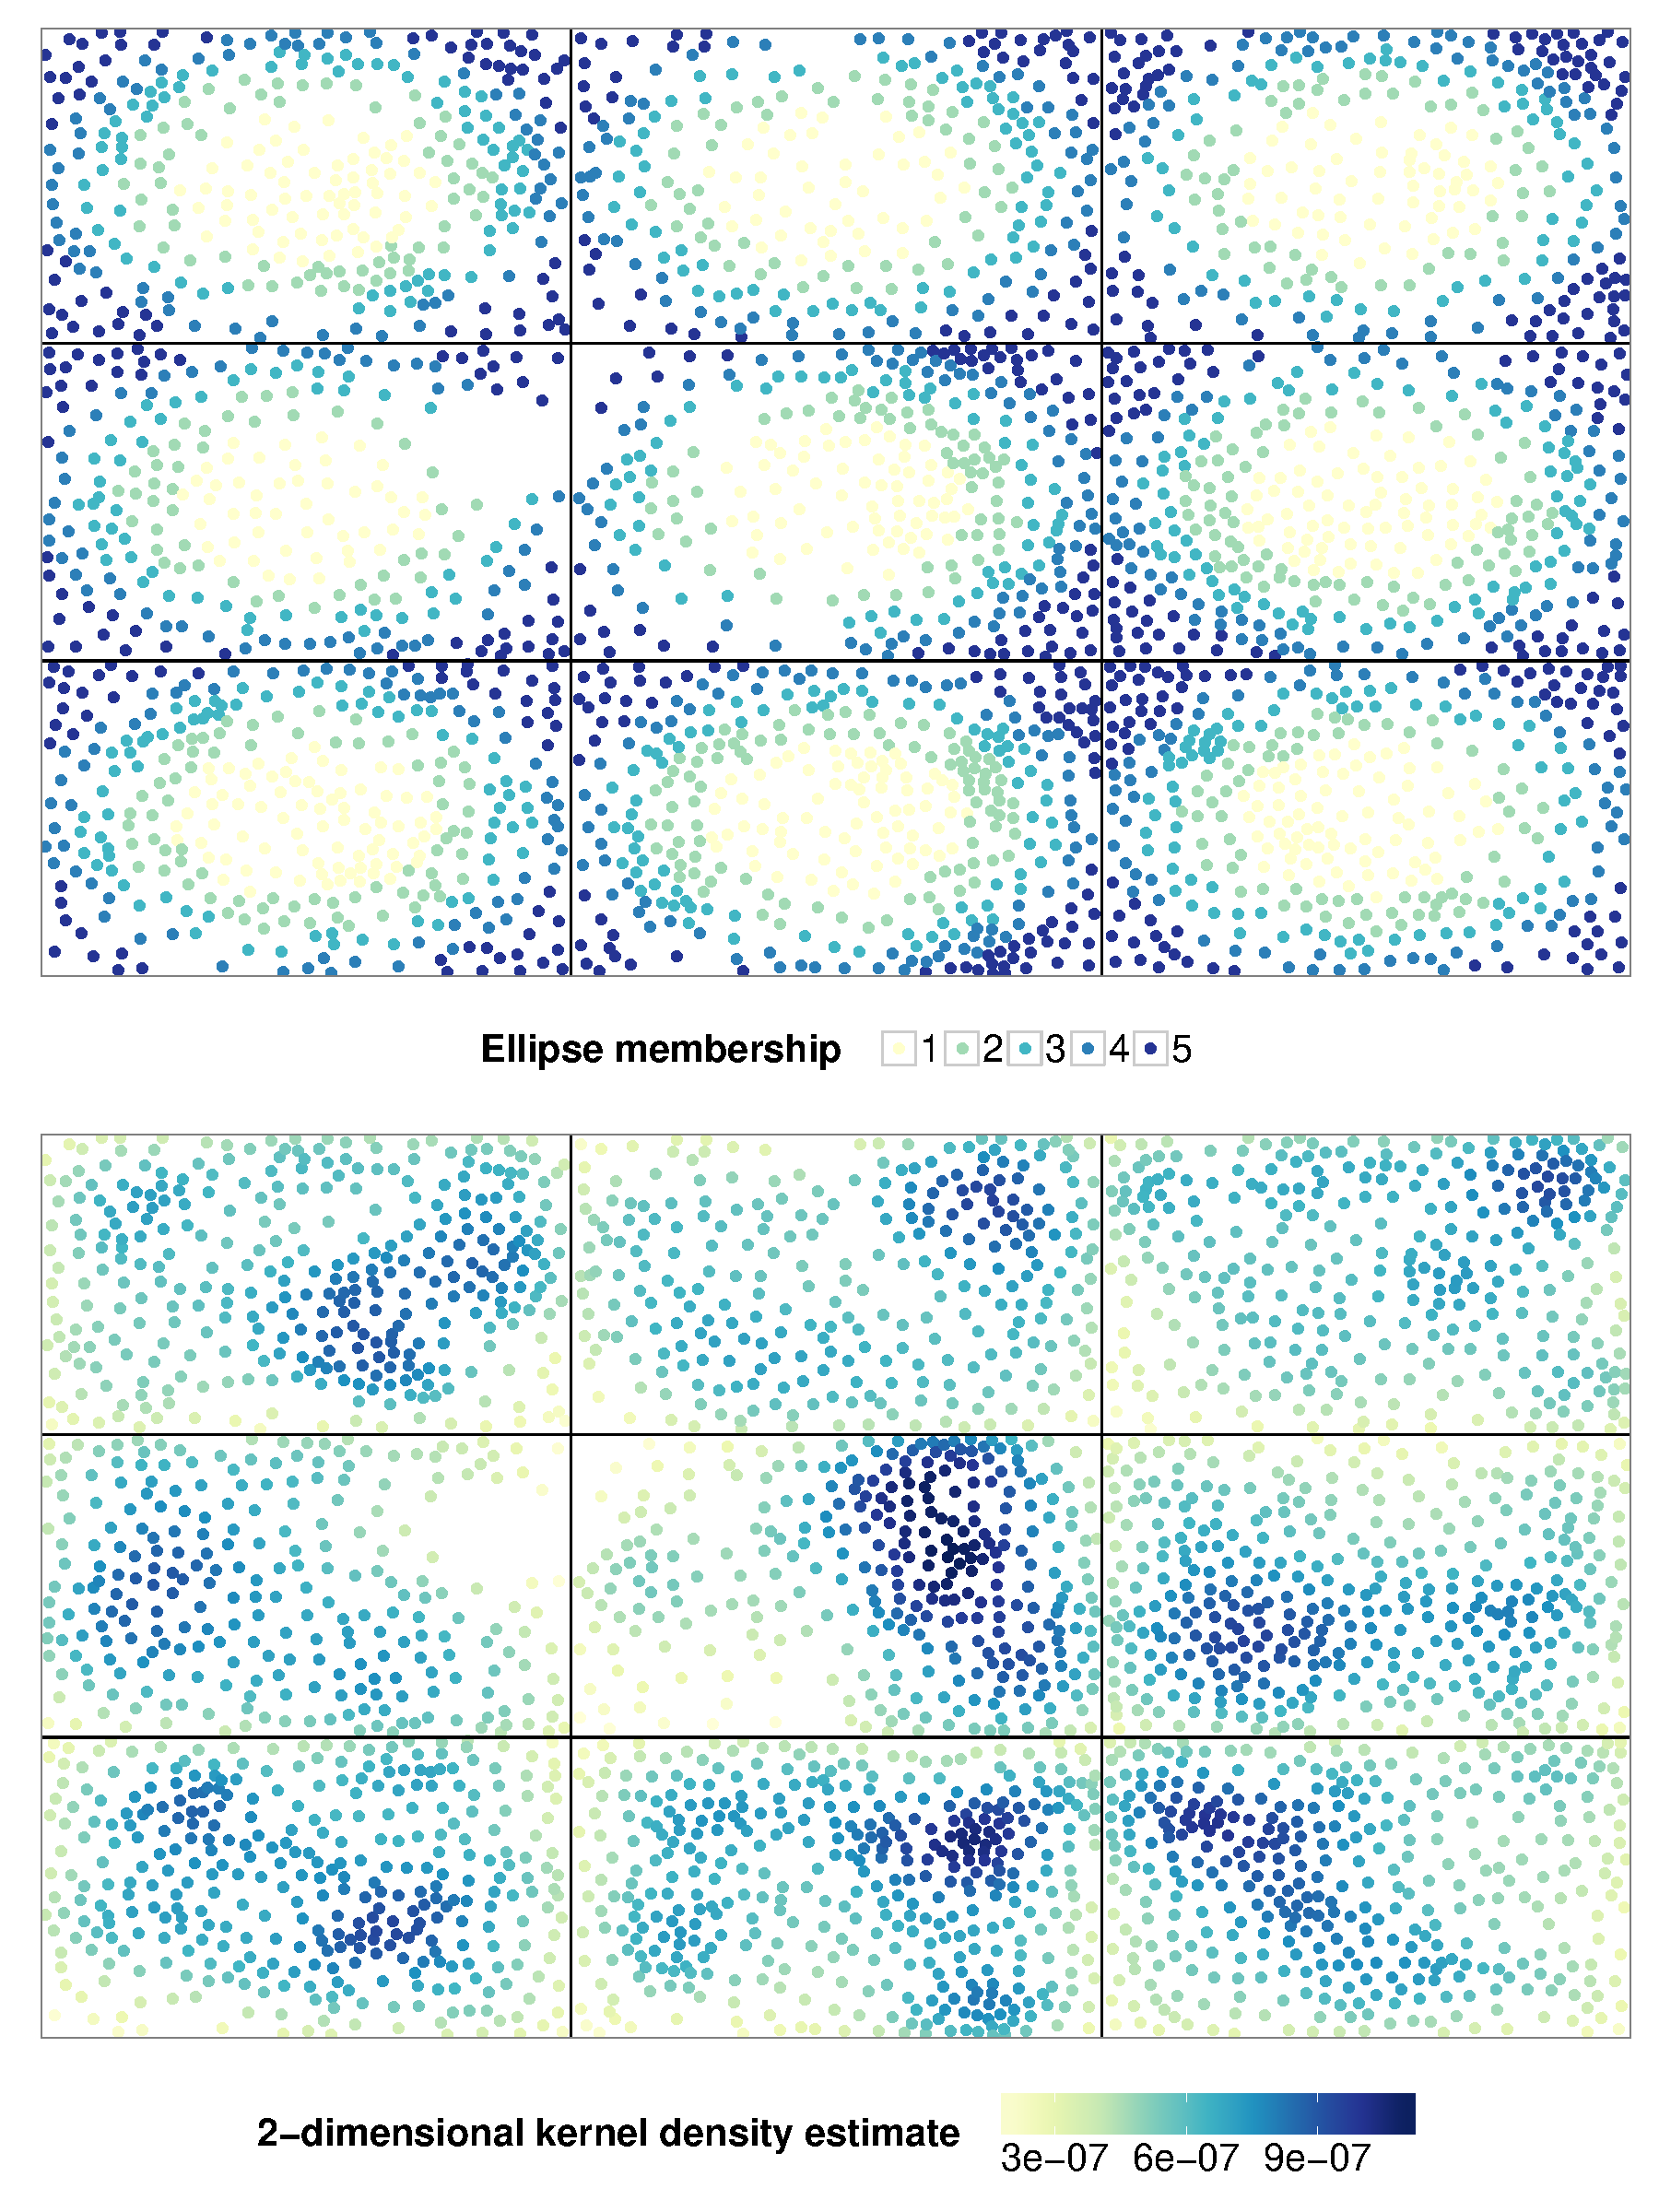
\includegraphics[width=.8\linewidth]{figures/R/augmentationFeatures-scf-augFeat_plot-1} 

}

\caption[Examples of coordinate augmentation functions as implemented in singleCellFeatures.]{Two examples of coorinate augmentation functions aiming at producing useful information from coordinates of cellular objects. The first image shows the discretized elliptic distance (5 bins of equal area) from individual image centers which could be relevant because of deteriorating optical properties of microscope lenses, while the second diagram visualized the 2-dimensional density of cellular objects, an important population context feature. Data is taken from well H6 of plate J107-2C.}\label{fig:scf-augFeat_plot}
\end{figure}


\end{knitrout}


\subsection{Feature Augmentation and Normalization}
Location features by themselves are useless, as they are represented as two vectors of individual coordinate values. If these coordinates, however are somehow contextualized, they hold the key to a considerable amount of information. Two examples of coordinate augmentation functions are visualized in figure \ref{fig:scf-augFeat_plot}. The top view is created by separating data points into concentric ellipses which might be relevant for normalizing against technical issues, such as optical properties of microscope lenses that degrade towards image borders (e.g. vignetting and sharpness). The bottom diagram shows 2-dimensional kernel density estimates as calculated by the CRAN package sm \citep{Bowman2014} which represents another population context feature as proposed by \cite{Knapp2011} and \cite{Snijder2012}.

Several additional features can be generated from object locations, all handled by \mintinline{text}{augmentCordinateFeatures}, including ellipses with respect to well center (instead of individual images centers), continuous distance from both image and well centers, as well as membership to 2-dimensional rectangular bins (both at well and image levels). Binning is accompanied by annotation with properties such as number of empty neighboring bins (see introductory example to this chapter) or their location within image and well (e.g. image border, image corner, image border that coincides with well border, image edge that is internal with respect to well, etc.).

The location of image within well can be used to generate a set of shifted coordinate features in order the describe object location not with respect to site, but well (calculated by \mintinline{text}{augmentImageLocation}). All these procedure have to be implemented in a very efficient manner, as they are used to process \tilde $10^6$ cells and cannot take more than seconds per feature in oder to be used interactively. Some aspects of this have already been covered earlier and while there is much more to discuss, the interested reader is directed to the publicly hosted \href{https://github.com/nbenn/singleCellFeatures}{source code}. All procedures can be applied at plate, well, and where applicable, at image level, owing to the S3 method dispatch system and the recursive implementation of data structures outlined in figure \ref{fig:scf-platedata}.

Another set of augmentation functions is directly aimed at data normalization. First there is \mintinline{text}{augmentAggregate}, which serves to calculate aggregate values on groups of objects (for example all cells in an image, all infected cells in a well or all pathogens throughout a plate). One argument that can be supplied as \mintinline{text}{func.aggr}, identifies an arbitrary function that produces a scalar from a vector of values (e.g. \mintinline{text}{min}, \mintinline{text}{max}, \mintinline{text}{mean}, \mintinline{text}{median}, \mintinline{text}{var}, \mintinline{text}{mad}, \mintinline{text}{sum}, etc.) and thusly performs the data summarization. An additional capability of note is the ability to include the 4 neighbors (north, east, south, west) when operating at well level in order to somewhat stabilize the results.

The function \mintinline{text}{augmentBscore} is only able to operate at plate level and produces row, column and plate effect estimates for each of the features specified by applying the \mintinline{text}{medpolish} procedure of the R stats package. Technical artifacts in \gls{hts} experiments can manifest as horizontally (for example due to a clogged pipette) or vertically striped patterns (e.g. degradation of microscope illumination) and B-scoring is a proven approach for correcting such issues. As is customary in B-scoring, control wells were originally excluded from the procedure. Unfortunately the way in which the layout of many InfectX plates is designed, this causes problems when control wells are to be used for analysis, as they occupy entire rows\slash columns for which the corresponding row and column effects are unavailable. Interleaving \gls{sirna} wells with control wells would alleviate the problem but place \gls{sirna} wells at the plate border, which is undesirable as well. Currently, control wells are included in B-scoring.

In order to perform data normalization itself, the user has two procedures at his disposal: \mintinline{text}{normalizeData}, which may be applied at every hierarchy level and \mintinline{text}{augmentMars}, which is only available to \mintinline{text}{PlateData} objects. The former function can accept regular expressions to specify the set of features it is to be applied to, as well as two sets of features that may have been generated by \mintinline{text}{augmentAggregate} for scaling and centering of the data. A small example might better convey what is possible with \mintinline{text}{normalizeData}:

\begin{rflow}
# fetch a complete plate dataset
data <- PlateData(PlateLocation("J107-2C"))
# discard any non-infected cells
data <- extractCells(data, infected=TRUE)
# regular expressions for selecting AreaShape, Intensity and Texture
# features of cellular objects
feat.sel <- c(".AreaShape_", ".Intensity_", ".Texture_")
feat.drp <- c("^Bacteria.", "^BlobBacteria.")
# calculate plate level median values for all selected features
data <- augmentAggregate(data, features=feat.sel, drop=feat.drp,
                         func.aggr="median", level="plate")
# calculate well level mad values for all selected features
data <- augmentAggregate(data, features=feat.sel, drop=feat.drp,
                         func.aggr="mad", level="well", neighbors=TRUE)
# normalize all selected values by robust Z-scoring
data <- normalizeData(data, select=feat.sel, drop=feat.drp,
                      values=".",
                      center="Aggreg_P_median$",
                      scale="Aggreg_N_mad$")
\end{rflow}

Any one of the center\slash scale parameters may be set to \mintinline{text}{NULL} and together with the flexibility of \mintinline{text}{augmentAggregate} a great range of possible normalization schemes can be applied. In this example a robust variant of Z-scoring is used, but only centering or scaling data is readily possible, as is using other summary functions (for example, \mintinline{text}{mean} and \mintinline{text}{var}, which would lead to regular Z-scoring).

One noteworthy implementation aspect is concerned with the great number of regular expressions that have to be executed. For each image, the set of selected features is iterated and within each iteration, the corresponding center and scale feature has to be found among the union of all available features (which, due to the non-destructive operation of all augmentation functions can grow up to 2000--3000). Furthermore, features are organized in a nested list (remember: at top level, they are sorted into \mintinline{text}{data.vec}, \mintinline{text}{data.mat} and \mintinline{text}{data.lst} categories and within each further subdivision into groups according to number of objects is possible). Constant traversal and matching of the same feature pairs (or triplets) is inefficient, as it is identical for all images. Therefore, a stencil of feature indices that specify locations within the nested structure, is precomputed and applied for each individual image. This optimization makes execution of a normalization scheme over a complete plate possible within \SI{90}{\second} for a setup as in the above example (only infected cells) or \SI{2}{\minute} for a full dataset.

The second normalization procedure, \mintinline{text}{augmentMars}, fits a fixed \gls{mars} model for each selected feature and returns the residuals as normalized feature values. Model fitting is performed by the CRAN package earth \citep{Hastie2015} and due to the large number of individual models that are involved, this is the most expensive operation in any singleCellFeatures analysis routine, taking on the order of \SI{25}{\minute} per plate. Normalization will be discussed more in depth in chapter \ref{ch:data-analysis}.

All augmentation and normalization functions operate in a non-destructive manner in the sense that they leave the original values intact and save results to copies of the features they were specified to operate on. In the above example, all features processed by the first application of \mintinline{text}{augmentAggregate} are saved with the added suffix \mintinline{text}{Aggreg_P_median}, which is used by \mintinline{text}{normalizeData} for identification as centering value. It is left to the user to discard sets of features that are no longer needed. While some space savings are possible, owing to the nested hierarchical model of \mintinline{text}{PlateData} structures (for example row and column effects of B-scoring do not have to be duplicated for every object, as would be the case in an entirely matrix based setup), objects holding several thousand features can become unwieldy. This is usually not a problem, as only a subset of original and derived features are needed leading to elimination of intermediate values by the user.

\subsection{Data Filtering}
Several functions for filtering datasets are available. Extraction of individual cells is possible via \mintinline{text}{extractCells} which may be applied at every plate, well or image level. Currently, the only available criterion is infection, but addition of a further group of parameters such as a vector of features, a set of order relations and corresponding thresholds could be added easily and would allow for arbitrary filtering with cellular granularity. At the next hierarchical tier, \mintinline{text}{extractImages}, available to \mintinline{text}{PlateData} and \mintinline{text}{WellData} objects, can be used to select individual images either keeping the superordinate data structure intact or discarding it, yielding a naked list. Finally, data extraction at well level is possible using \mintinline{text}{extractWells}, which owing to circumstance is only available to plate objects. Again the the user may keep the encompassing plate structure or throw it out.

Dropping or extracting a subset of features may be accomplished by calling the function \mintinline{text}{extractFeatures} on any type of \mintinline{text}{Data} structure. Either a vector of regular expressions can be used to select features, followed by application of a further vector of regular expressions for removing erroneously selected instances, or a vector of feature names can be supplied that is matched exactly. Again, for performance reasons, when run at plate scale, the large number of repeated regular expressions causes speed issues and in such cases, the feature names are worked out once for the first and reused in all subsequent wells.

The function \mintinline{text}{cleanData}, which may act on plates and wells, is currently used for eliminating image sites with very few or too many cellular objects. This measure serves to combat segmentation issues and eliminate some technical artifacts such as bad focus. Images are selected according to image-level cell count quantiles and the user can choose whether to do away with only the upper or lower 5\%, or discard data symmetrically. Having well quality annotation metadata available, the procedure is planned to be extended to also remove wells that carry the label \mintinline{text}{BAD} but as of yet this has not been a priority due to the predominance of missing labels.

Further, related functionality is provided by \mintinline{text}{makeFeatureCompatible}, which can be used to ensure that multiple \mintinline{text}{Data} objects, supplied as a list, share the same features. For dealing with data heterogeneity, the intersection of individual feature sets is computed using the base function \mintinline{text}{Reduce} and subsequently extracted from each object. In order to illustrate the brevity with which such procedures can be implemented owing to R's broad range of library functions, coupled with convenience functions available to singleCellFeatures, the source to this function is reproduced in listing \ref{lst:feature-compat}. This procedure can be applied to any combination of \mintinline{text}{PlateData}, \mintinline{text}{WellData} and \mintinline{text}{ImageData}, owing to generic functions and the S3 method dispatch system.

\subsection{Ensuring Dataset Consistency}
Despite efforts to design data structure modifying functions in such a way that prevents introducing inconsistencies, there if no formal safe-guarding and due to how S3 objects are designed, the user can do whatever he pleases (for example removing features only in a subset of wells). Therefore, several procedures exist, that can be used to ensure that some assumptions made throughout the code base (such as an identical set of features throughout a plate) still hold. Checking whether the set of features per se is complete can be done with \mintinline{text}{checkCompletenessFeature}, which has been introduced earlier as the function that checks \mintinline{text}{PlateData} objects before well caches are written and reports on the state of \mintinline{text}{MatData} caches following their retrieval.

\begin{rlisting}{float=t}{The function \mintinline{text}{makeFeatureCompatible} can be used to ensure an identical feature set among the supplied objects.}{Used for reducing the supplied list of objects to the common set of features, this function serves as an illustration of the conciseness that is possible due to R's range of library functions coupled with functionality implemented in singleCellFeatures.}{feature-compat}
\begin{rcode}
makeFeatureCompatible <- function(lst) {
  # input validation
  stopifnot(sapply(lst, function(x) any(class(x) == "Data")))
  # check objects for internal consistency
  stopifnot(sapply(lst, checkConsistency))
  # get individual feature lists
  features <- lapply(lst, getFeatureNames)
  # produce intersection of feature lists
  intersection <- Reduce(intersect, features)
  # extract intersection from each object
  res <- lapply(lst, extractFeatures, features=intersection)
  return(res)
}
\end{rcode}
\end{rlisting}

Both functions \mintinline{text}{checkCompletenessImage} and \mintinline{text}{checkCompletenessWell} are concerned with structural integrity of the respective structures in the sense that they contain the expected number of sub-structures. In case of images, two possibilities exist, which have to be handled, whereas plates are currently fixed to a 384 well-layout. Finally, \mintinline{text}{checkConsistency} is slightly more involved, as no fixed template exists that can be matched. At well level, the method builds an image-level prototype consisting of metadata such as well name, plate barcode and the structuring of features alongside feature names themselves and compares this among all images. At plate level, the procedure is applied recursively, and requires 384 additional comparisons to check coherence among wells.

Listing \ref{lst:feature-compat} contains an example application of a consistency check, which is required due to reliance on \mintinline{text}{getFeatureNames}. As this function is employed in several speed-critical settings, it simply extracts the feature set of a single image and does not check if every other image contains the same set of features. Due to the intent behind \mintinline{text}{makeFeatureCompatible} this however has to be enforced.

\subsection{Data Melting\footnote{Naming of this functionality is inspired by the pair of functions \mintinline{text}{cast} and \mintinline{text}{melt}, provided by the CRAN package reshape2 \citep{Wickham2007}.}}
One of the most important functions for every analysis procedure that relies on external tools, is \mintinline{text}{meltData} which turns the supplied \mintinline{text}{Data} structure into the smallest possible set of \mintinline{text}{data.frames} (see listing \ref{lst:meltdata}). At image level, the data representation does not have to be significantly altered apart from merging of some metadata fields into the data nodes in preparation of loss of structure conveying this information (examples include image and well indices, as well as plate barcode). At well level, the corresponding data structures are combined using \mintinline{text}{rbind} (for \mintinline{text}{vec} and \mintinline{text}{mat} features), while the \mintinline{text}{bdiag} function (from the Matrix package) is used for creating block diagonal adjacency matrices.

Well metadata is written into a special group under the \mintinline{text}{vec} node, thereby avoiding replication and consequent storage blowup (see listing \ref{lst:meltdata}, line 8 and following). A similar procedure for both storing metadata and concatenating subordinate data-structures is applied at plate level, yielding a nested list grouped by top level slots \mintinline{text}{vec}, \mintinline{text}{mat} and \mintinline{text}{lst}, which are further subdivided into \mintinline{text}{data.frames} corresponding to objects with different counts (Bacteria, BlobBacteria and Cells in case of the \mintinline{text}{mat} node shown in listing \ref{lst:meltdata}).

\afterpage{\clearpage\begin{rlisting}{nofloat}{Output structure of a complete plate as returned by \mintinline{text}{meltData}.}{While not a proper code listing, this represents a heavily truncated output view as produced by applying \mintinline{text}{str} on the result returned by \mintinline{text}{meltData} after having processed a complete plate.}{meltdata}
\begin{rcode}
List of 3
 $ vec:List of 3
  ..$ Image:'data.frame': 3456 obs. of  32 variables:
  .. ..$ Image.Count_Bacteria    : num [1:3456] 289 156 137 19 0 62 36 37 ...
  .. ..$ Image.Count_BlobBacteria: num [1:3456] 288 125 137 19 0 46 29 25 ...
  .. ..$ Well.Index              : num [1:3456] 1 1 1 1 1 1 1 1 1 2 ...
  .. .. [list output truncated]
  ..$ Well :'data.frame': 384 obs. of  15 variables:
  .. ..$ Well.Index     : num [1:384] 1 2 3 4 5 6 7 8 9 10 ...
  .. ..$ Well.Gene_ID   : chr [1:384] "523" "none" "none" "none" ...
  .. ..$ Well.siRNA_Name: chr [1:384] "ATP6V1A" "SCRAMBLED" "MOCK" "MOCK" ...
  .. .. [list output truncated]
  ..$ Plate:'data.frame': 1 obs. of  6 variables:
  .. ..$ Plate.Barcode  : chr "J101-2C"
  .. ..$ Plate.Quality  : chr "UNKNOWN"
  .. ..$ Experiment.Name: chr "BRUCELLA-DU-K1"
  .. .. [list output truncated]
 $ mat:List of 3
  ..$ Bacteria    :'data.frame':  388625 obs. of  51 variables:
  .. ..$ Bacteria.AreaShape_PerObjArea_CorrPathogen      : num [1:388625] ...
  .. ..$ Bacteria.Intensity_MassDisplacement_CorrPathogen: num [1:388625] ...
  .. ..$ Well.Index                                      : num [1:388625] ...
  .. .. [list output truncated]
  ..$ BlobBacteria:'data.frame':  222981 obs. of  7 variables:
  .. ..$ BlobBacteria.Location_Center_X: num [1:222981] 1.25 42.45 3 5 6.33 ...
  .. ..$ BlobBacteria.Location_Center_Y: num [1:222981] 130 210 119 111 138 ...
  .. ..$ Well.Index                    : num [1:222981] 1 1 1 1 1 1 1 1 1 1 ...
  .. .. [list output truncated]
  ..$ Cells       :'data.frame':  945851 obs. of  529 variables:
  .. ..$ Cells.AreaShape_Area        : num [1:945851] 141389 2104 2466 ...
  .. ..$ Cells.AreaShape_Eccentricity: num [1:945851] 0.893 0.554 0.928 ...
  .. ..$ Cells.AreaShape_EulerNumber : num [1:945851] 1 1 1 1 1 1 1 1 1 1 ...
  .. .. [list output truncated]
 $ lst:List of 2
  ..$ IdentityOfNeighbors     :List of 3
  .. ..$ Neighbors.IdentityOfNeighbors_Cells_2
                 :Formal class 'lgCMatrix' [package "Matrix"] with 6 slots
  .. .. .. ..@ i       : int [1:4746004] 8 4 7 2 6 9 19 4 9 10 ...
  .. .. .. ..@ p       : int [1:945843] 0 1 1 2 3 6 7 11 12 13 ...
  .. .. .. ..@ Dim     : int [1:2] 945842 945842
  .. .. .. ..@ Dimnames:List of 2
  .. .. .. .. ..$ : chr [1:945842] "A1_2" "A1_2" "A1_2" "A1_2" ...
  .. .. .. .. ..$ : NULL
  .. .. .. ..@ x       : logi [1:4746004] TRUE TRUE TRUE TRUE TRUE TRUE ...
  .. .. .. ..@ factors : list()
  .. .. [list output truncated]
  .. [list output truncated]
\end{rcode}

\end{rlisting}}

Acting on the structure resulting from running \mintinline{text}{meltData}, is the utility function \mintinline{text}{moveFeatures}, which is capable of relocating features between nodes \mintinline{text}{vec}, \mintinline{text}{mat} and \mintinline{text}{lst}. It can be used, for example, when a metadata feature, such as gene name needs to be available per cell, or the opposite way round, when a cellular feature should be included in the matrix representing per well features. Whether the selected data vectors have to be expanded, or collapsed, the function automatically determines which replication pattern to use or how to aggregate data (using the specified summary function) in order to meet the target dimensions. In practice, this is of great usefulness, combining space saving attributes of the molten data structure with the ability to expand user selected features for simplified interface with external procedures.

\section{Utility and Convenience Functions}
A multitude of specialized convenience functions for working with the described S3 objects were developed alongside to the functionality discussed above. Much of this code is used internally throughout the project, and where sensible, the methods are exported to the package namespace and hence made available to the user. Examples are functions for visualizing data, utilities for managing the package and cache objects, various getter functions to directly access and extract certain information from custom classes and conversion procedures for certain object pairs. Due to diversity and extent these additional features unfortunately cannot be covered in their entirety and only a selection is highlighted and briefly discussed.

\paragraph{Visualization.}
Heatmaps and box-plots can be used to visualize certain features in a plate wide context and bubble plots at a single image level are currently under development. An exemplary view, resulting from applying the function \mintinline{text}{plateHeatmap} to the feature Nuclei.AreaShape\_Area, aggregating data at well level by calculating the mean and using a logarithmic color scale is shown in figure \ref{fig:scf-heatmap}. Control wells are marked by black borders, while actual \gls{sirna} experiments are indicated by white rectangles. Tile coloring can be specified by supplying the function with a vector of colors that is interpolated to produce a gradient and the color scale is chosen by a function valued parameter (e.g. \mintinline{text}{identity} which is default, \mintinline{text}{log} or \mintinline{text}{sqrt}), while the data summary method is indicated analogously (e.g. \mintinline{text}{mean}, \mintinline{text}{median}, \mintinline{text}{var}, \mintinline{text}{mad}, etc.).

Plate-level box plots are a bit unwieldy for print media, are therefore not shown, but provide a useful method of spotting wells which might contain untrustworthy data. Bubble plots, thought for overlaying individual images with some feature data are partially implemented but the automatic image fetching from openBIS still requires some work. Such visualizations are primarily used for validating sensibility of feature data, by providing side-by side comparison with raw image data.

\begin{knitrout}
\definecolor{shadecolor}{rgb}{0.969, 0.969, 0.969}\color{fgcolor}\begin{figure}

{\centering 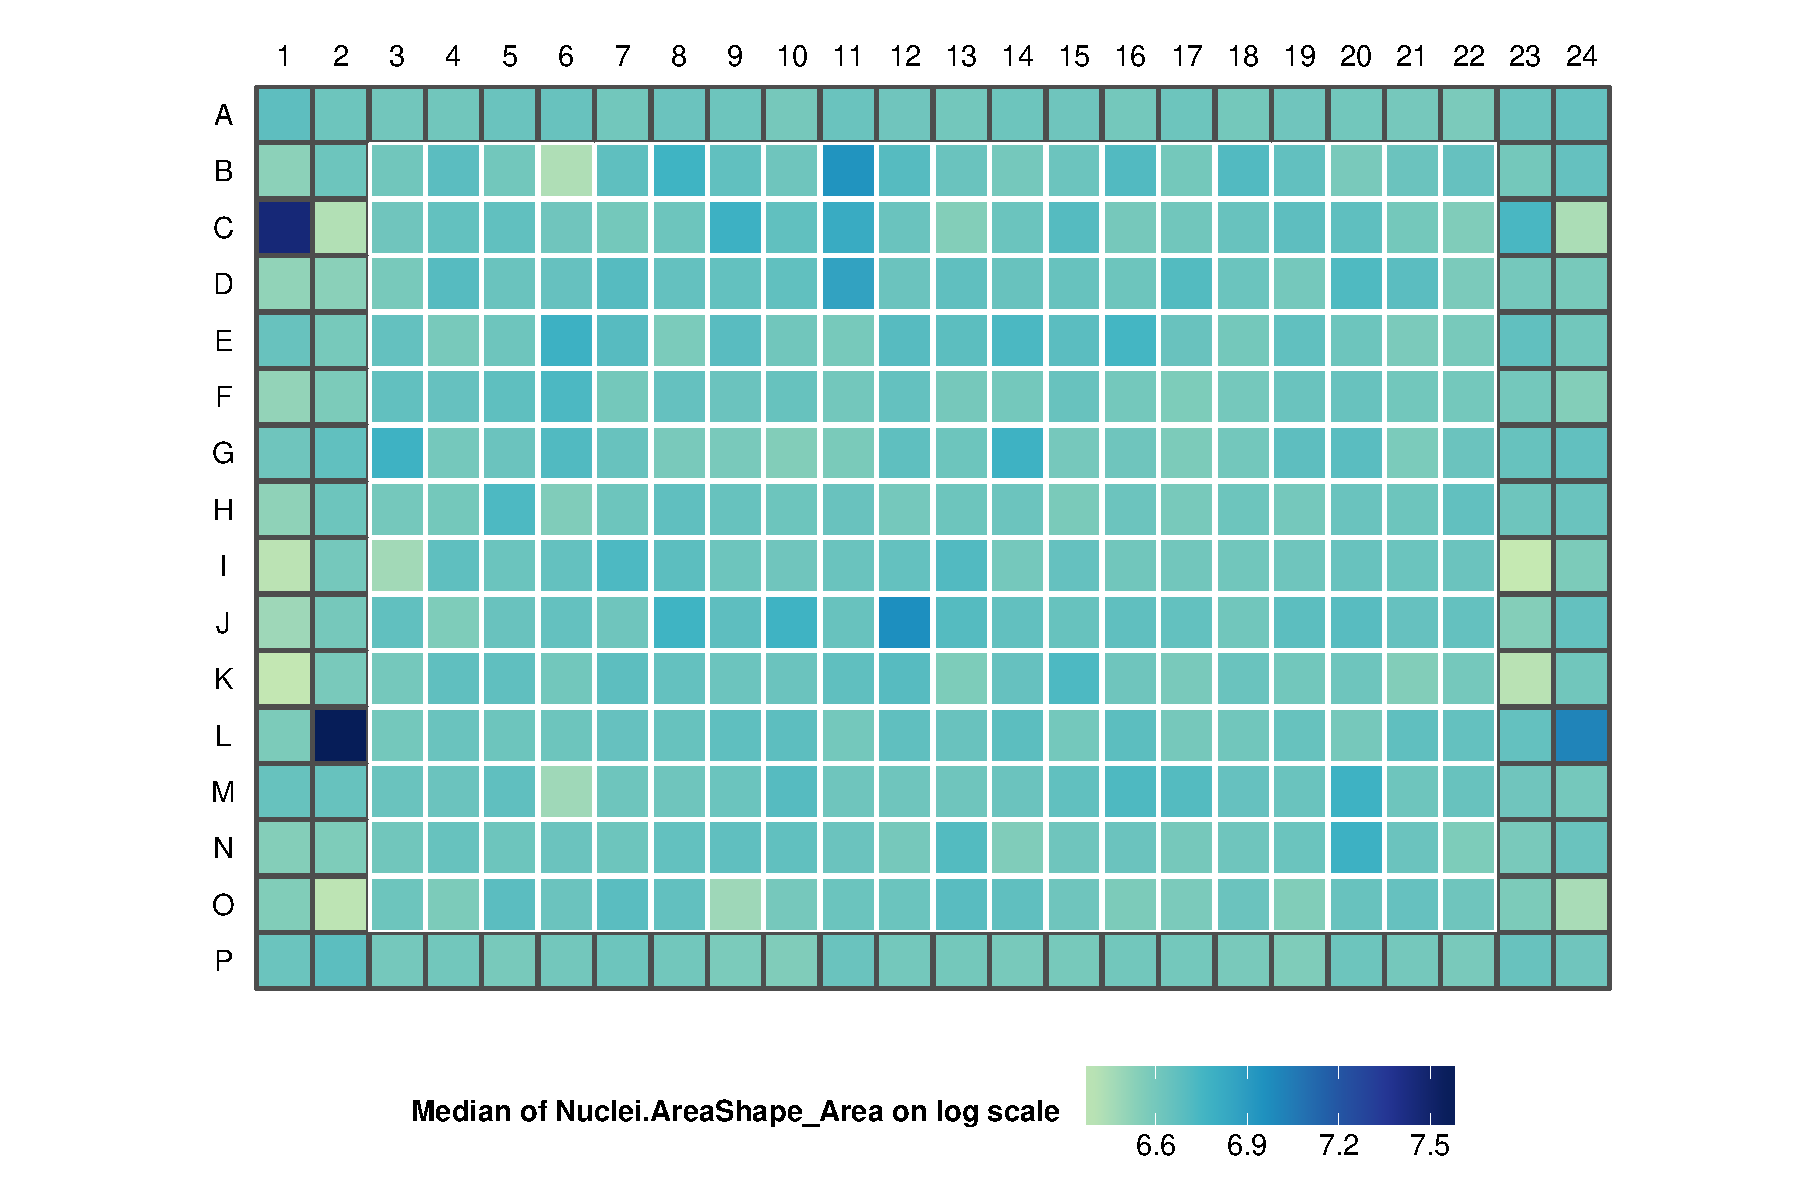
\includegraphics[width=.95\linewidth]{figures/R/heatmap-demo-scf-heatmap-1} 

}

\caption[An example heatmap plot as produced by \mintinline{text}{plateHeatmap}.]{Several visualization procedures are integrated with singelCellFeatures. In this example, the median of the feature Nuclei.AreaShape\_Area is shown on a logarithmic scale. Two parameters of \mintinline{text}{plateHeatmap} are functions so that the user can customize both, how data per well is summarized and on what scale colors are determined. The plate is J101-2C (wells C1, L2, C23 and L24 contain cell killer \gls{kif11} \gls{sirna}).}\label{fig:scf-heatmap}
\end{figure}


\end{knitrout}


\paragraph{Package utilities.}
Functions of this group have been mentioned in several places and comprise of tools for metadata coverage assessment, configuration management, cache updating and invalidation, as well as database management. A report on the discrepancy between plates that have single cell features available and datasets that are represented by metadata is generated each time the package is attached to an R session (using the \mintinline{text}{.onLoad} hook). The corresponding function, run as \mintinline{text}{wellDatabaseCoverage(TRUE)} can be used to display a detailed overview of current metadata coverage at well level which is particularly important for searching.

Configuration management relies on a yaml based file used storing system specific parameters (see section \ref{sec:install-package}). Setter functions, as well as getters for location and content, in addition to an initiation routine that sets up an empty template for user editing, are available for its manipulation and access.

In order to curate the lookup tables used for search and various speed critical, metadata dependent processes, each database type has a corresponding update function available (\mintinline{text}{updateDatabaseFeatures}, \mintinline{text}{updateDatabasePlate} and \mintinline{text}{updateDatabaseWells}). As all metadata available to singleCellFeatures is static and does not reflect new additions to openBIS, section \ref{sec:update-metadata} describes how to update the underlying files and the above tools can recreate the databases using updated source data.

While cache-related functionality has primarily been covered from a perspective of creation and retrieval, several additional functions for managing the set of cached objects are at the users disposal. Metadata and well caches can be flushed (rebuilding is comparably cheap) and reports on the extent of plate level caches can be compiled. Moreover, \mintinline{text}{rebuildAllMatDataCaches} implements a procedure that iterates all plate cache objects and determines if any improvements are available. This can be used, for example after batch-downloading many plates to trigger retry of features that failed to import in applicable plates, or in case some features did not download, selectively initiate re-fetching. A further application is if new features become available, the function can be used to specifically start the respective downloads and imports into existing objects eliminating the need of having to re-process affected plates completely (which is an expensive operation).

Furthermore, for the package to be usable in a cluster environment, resource allocation has to be respected. Parallelized sections are using foreach \citep{Weston2014} alongside the doParallel backend \citep{Weston2014a} and it needs to be ensured that forked processes only run on the allowed cores. The function \mintinline{text}{getNumCores}, for example, can be used to determine the number of available cores by either reading the corresponding environmental variable set by Platform LSF, or by using \mintinline{text}{detectCores} of doParallel.

\begin{rlisting}{float=t}{A convenience function that converts its argument into a \mintinline{text}{PlateLocation} object.}{Many convenience functions are available to singleCellFeatures, one of which can be used to convert its argument into a \mintinline{text}{PlateLocation} object. A further example of such a simple, single purpose method is the getter function \mintinline{text}{getBarcode}, which extract the barcode from the object it is called upon.}{convert}
\begin{rcode}
convertToPlateLocation <- function(x) {
  UseMethod("convertToPlateLocation", x)
}

convertToPlateLocation.DataLocation <- function(x) {
  barcode <- getBarcode(x)
  return(PlateLocation(barcode))
}

convertToPlateLocation.Data <- function(x) {
  barcode <- getBarcode(x)
  return(PlateLocation(barcode))
}

convertToPlateLocation.PlateAggregate <- function(x) {
  return(x$plate)
}

convertToPlateLocation.default <- function(x) {
  stop("can only deal with PlateData/MatData/WellLocation objects.")
}
\end{rcode}
\end{rlisting}

\paragraph{Convenience functions.}
This section covers a diverse range of methods including many getters for S3 objects and short, narrow purpose functions for common tasks. It is unfitting to describe these tools in their entirety and the interested reader is encouraged to look at the publicly hosted source code, or look though the manual pages that come with the package and are browsable through the R help system. Listing \ref{lst:convert} shows one instance of such a function which can be used to create a \mintinline{text}{PlateLocation} object out of the supplied data structure, thereby converting the argument into a plate location specification. The example on page \pageref{ex:dataobject-instantiation} provides a real-world application of such a conversion function.

The reasoning for using multiple description attributes for objects can be illustrated by means of this code excerpt:\footnote{As a reminder, for instance, both \mintinline{text}{PlateLocation} and \mintinline{text}{WellLocation} are also \mintinline{text}{DataLocation} objects and the same pattern holds for other groups of S3 classes.} As the function \mintinline{text}{getBarcode} (one of the aforementioned getter functions) is defined for all \mintinline{text}{Data} classes, four functions acting on \mintinline{text}{MatData}, \mintinline{text}{PlateData}, \mintinline{text}{WellData} and \mintinline{text}{ImageData} can be written as one by creating this additional level of hierarchy in object type naming, thereby reducing redundant code. In this case, one could even combine the functions that act on \mintinline{text}{DataLocation} and \mintinline{text}{Data} objects if an attribute grouping those classes were available. However, to avoid overly complex attribute relationships, only functionally related classes are gathered.

\paragraph{Interface to \acrshort{glm} routines.}
Currently still under development, several functions that interface with \gls{glm} routines are available to the user. Originally intended for building a model that discriminates two gene knockdown experiments based on single cell features, the function \mintinline{text}{prepareDataforGlm} can take two lists of wells and make the data ready for analysis with \gls{glm} by concatenating and annotating the wells with a response vector. Additional options are sampling based splitting of data into testing and training sets and dropping of features that by themselves separate the data into the two knockdown groups.

Due to issues in logistic regression, caused by data that is separated into the two groups that are modeled by a hyperplane, \mintinline{text}{analyzeSeparation} can be used for preliminary investigation of this aspect. The procedure will first check if individual features separate the data, followed by looking at all $n \choose 2$ pairs of features. Unordered \textit{k}-tuples may be explored up to a user defined threshold but with several 100 features to be considered, the number of sets resulting from $k > 2$ becomes prohibitively large and the function will skip iteration k and above if ${n \choose k} > 250000$. In a final step, all features are considered simultaneously, solving the problem with a linear programming approach, using the CRAN package lpSolveAPI \citep{Konis2007,Konis2014}. A further data issue that has to be dealt with is rank deficiency and the procedure \mintinline{text}{makeRankFull} can be used in this capacity. Features that either have zero variance or comprise of highly correlated columns, are removed prior to analysis.

A parallelized function for investigating the stability of the largest n coefficients in \gls{glm}, the set of features as determined by stepwise \gls{glm}, or the set of nonzero coefficients in regularized \gls{glm} analysis is available as the function \mintinline{text}{glmBootstrapStability}. For both stepwise and plain \gls{glm}, the functions \mintinline{text}{glm} and \mintinline{text}{step} of the R stats package are used, while regularized fitting is performed by \mintinline{text}{glmnet} \citep{Friedman2010a}. A user specified fraction of the data (default 0.7) is sampled in each iteration and the resulting coefficients are stored for subsequent counting and tabulation. Unfortunately, there currently are unresolved issues regarding data normalization, making this type of analysis infeasible. Therefore all \gls{glm} oriented routines are subject to change.


\chapter{Data Analysis}
\label{ch:data-analysis}

The initial goal of this master's thesis was concerned with modeling different infection patterns as influenced through \cgls{sirna} mediated gene knockdown. By fitting a \cgls{glm} model, using the large set of available cellular features, described in section \ref{sec:scf-data}, as predictor variables and the membership to one of two wells as binary response, it was conjectured that it is possible to determine a subset of most influential features. Unfortunately, to present date, this could not be executed in a sensible manner.

In order the make the substantial amount of single cell data, obtained from several large-scale, high throughput \cgls{sirna} screens performed by the InfectX consortium, available to an environment for statistical analysis, an R packages was developed, which is described in chapter \ref{ch:singlecellfeatures}. Building on this crucial piece of infrastructure, the current chapter will explore some of the data analysis that was performed, beginning a short introduction into the theory of \cglspl{glm} and continuing with preliminary findings that motivate the investigation of desirable normalization schemes. A final outlook on potential improvements will conclude this chapter.

\section{Statistical Models}
Many algorithms for binary classification exist, including decision trees, \cglspl{svm}, Bayesian networks, neural networks and \cglspl{glm}, some of which have been encountered in previous sections due to their application in infection scoring (see section \ref{sec:infection-scoring}). As neither prediction not classification per se are of main interest, binary logistic regression presents an attractive method due to availability of closed-form coefficient and model statistics. Therefore, modeling of \cgls{sirna} effects on cellular features is performed, using the glm function provided by the R stats package \citep{RCoreTeam2015}.

A large number of binary comparisons are possible with the given datasets. In order to focus on attractive wells in the sense that there is reason to assume they might be biologically interesting, the $n \choose 2$ possible combinations of wells (within a single plate, where $n=384$, \tilde 70000 pairs can be formed), are narrowed down using a \cgls{pmm} as derived by \citet{Ramo2014}. Of the resulting hit list, several genes are selected and compared to wells containing scrambled \cgls{sirna} reagents, which should provide a good choice for usage as control. A possible alternative to scrambled experiments are mock wells but owing to the complete absence of \cgls{sirna} molecules, the difference in treatment of cells is only increased and hence it can be argued that they provide biased comparisons.

\subsection{Generalized Linear Models}
Modeling the relationship among variables is one of the most important applications of statistical theory. The study of regression analysis (and the closely related notion of correlation) started to form towards the end of the 19th century with Sir Francis Galton's study of height heredity in humans and his observation of regression towards the mean. Over the next few years, Udny Yule and Karl Pearson cast the developed concepts into precise mathematical formulation, in turn building on work performed by Adrien-Marie Legendre and Carl Friedrich Gauss who developed the method of least squares almost a century earlier \citep{Allen1997}.

A multiple linear regression model can be written in matrix-vector form as
\begin{equation}
  y = X \beta + \epsilon \label{eq:lin-reg}
\end{equation}
where $y \in \R^n$ is the vector of observations on the dependent variable, the design matrix $X \in \R^{n \times p}$ contains data on the independent variables, $\beta \in \R^p$ is the $p$-dimensional parameter vector and the error term $\epsilon \in \R^n$ captures effects not modeled by the regressors.

In order to estimate unknown coefficients $\beta_i$, the ordinary least squares estimator minimizes the residual sum of squares, the squared differences between observed responses and their predictions according to the linear model.
\begin{subequations}
\begin{align}
  \Hbeta &= \argmin_{\beta} \norm{y - X \beta}^2 \\
         &= (X^T X)^{-1} X^T y \label{eq:ols-estimate}
\end{align}
\end{subequations}
Some assumptions are typically associated with linear regression models that yield desirable attributes for the estimates (e.g. statistical tests of significance). None of these restrictions are imposed on the explanatory variables; they can be continuous or discrete and combined as well as transformed arbitrarily. Furthermore, in practice, it is irrelevant whether the covariates are treated as random variables or as deterministic constants. With exception of the field of econometrics it appears that the majority of literature adheres to the latter interpretation and therefore, statements will not explicitly be conditional on covariate values.
\begin{description}
  \item[Linearity.] The relationship between dependent and independent variables is assumed to be linear in coefficients (after suitable transformations of regressors) and individual effects additive. If this cannot be satisfied, a linear model is not suitable.
  \item[Full rank.] For the matrix $X^T X$ to be invertible, it has to have full column rank $p$. Therefore $n \geq p$ and all covariates must be linearly independent.
  \item[Exogeneity.] All independent variables should be known exactly i.e. contain no measurement or observation errors as only the mean squared error of the dependent variable is minimized. Additionally, all important causal factors have to be included in the model. Exogeneity implies $\E[\epsilon_i] = 0 \forall i$, as well no correlation between regressors and error terms \citep{Hayashi2000}.
  \item[Spherical errors.] This includes both homoscedasticity or constant error variance, $\E[\epsilon_i^2] = \sigma^2 \forall i$, and uncorrelated errors $\E[\epsilon_i \epsilon_j] = 0 \forall i \neq j$. These two conditions can be written more compactly as $\Var(\epsilon) = \sigma^2I_{n \times n}$.
  \item[Normality.] For the estimated coefficients to gain some additional desirable characteristics, it can be required that the errors $\epsilon_i$ be jointly normally distributed. Together with the above restrictions on expectation and variance, this yields $\epsilon \mathbin{\sim} \N_n(0, \sigma^2 I_{n \times n})$.
\end{description}

Violations of these assumptions have varying consequences. In situations of perfect collinearity, the ordinary least squares estimator $\Hbeta$ as defined in \eqref{eq:ols-estimate} does not exist. Recovering such a situation is possible by using a generalized matrix inverse (for example the Moore--Penrose pseudoinverse) or by dropping the corresponding variables. High correlation inflates coefficient variances, which may be countered by employing a regularization scheme like ridge regression. Failure to fulfill exogeneity, for example by omitting relevant explanatory variables, leads to regressors that are correlated with the error term, which in turn yields invalid (biased and inconsistent) \cgls{ols} estimates. The method of instrumental variables can help to produce an unbiased estimator nonetheless.

The assumption of spherical errors ensures that the least squares estimator is the best linear unbiased estimator in the sense that it has minimal variance among all linear unbiased estimators. Heteroscedasticity and autocorrelation do not yield biased coefficient estimates but can introduce bias in \cgls{ols} estimates of variance, causing inaccurate standard errors. Such a situation calls for generalized least squares estimation, such as weighted least squares for when the data is not homoscedastic ($\sigma^2$ is vector-valued but off-diagonal elements of $\Var(\epsilon)$ are zero), or feasible generalized least squares which can be applied in case of heteroscedasticity and\slash or correlation between errors. Whenever the condition of spherical errors does not hold, \cgls{ols} is inefficient and generalized least squares estimators have smaller variance.

Finally, normality provides the framework necessary for applying common hypothesis testing, yielding t-statistics, p-values and confidence intervals for coefficients, as well as an F-statistic for the model as a whole. Furthermore, under normality assumptions, the \cgls{ols} estimator and \cgls{mle} coincide. Quantile regression and other forms of robust regression, such as M estimators may restore validity of inference when errors do not follow a normal distribution.

Modeling data to a dichotomous response variable with \cgls{ols} methodology, while readily possible, often is a bad choice due to violations of several of the above assumptions. First of all, normal distributions are continous with support $x \in \R$ and thusly a categorical variable cannot be normally distributed. Homoscedasticity does not hold either, as can easily be seen in a geometric argument: any line with nonzero slope, fitted to a set of $Y$ with $Y_i \in \{0,1\}$, will produce residuals that vary linearly. Finally and perhaps most importantly, a linear model is unsuitable due to missing constraints on the range of fitted values. While this by itself could be dealt with, the concept of additivity within this context raises questions of its own when fitted values are thought of as probabilities. Linear behavior throughout the range of 0 (impossible) to 1 (certain) makes little sense for most practical applications, as typically, some flattening is expected when approaching either end of the spectrum.

In view of the above considerations it becomes clear that some sort of extension to ordinary linear regression is needed in order to deal with binary response variables. A theory, unifying several previously separately treated statistical models, including linear regression, \cgls{anova}, logistic regression, Poisson regression and multinomial response, was developed by John Nelder, Robert Wedderburn and Peter McCullagh in the early 1970's \citep{Nelder1972,McCullagh1989} and is known as \acrfull{glm}. Much of this section is based on \citep{McCullagh1989}.

In order to accommodate the newly added extensions, the classical linear model is rewritten as

\begin{equation}
  \E[Y] = \mu \text{ where } g(\mu) = \eta \text{ and } \eta = X \beta,
\end{equation}

yielding a three-part specification, consisting of

\begin{enumerate}[label=(\alph*)]
  \item the \textit{random component}; $Y$ is distributed according to a member of the exponential family,\footnote{Many of the predominately used distributions belong to the exponential family, including but not restricted to Bernoulli, binomial, Poisson, exponential and normal distributions. Common to all members, the probability density function can be written as
  \begin{equation}
    f(x;\theta) = h(x) e^{\theta^\intercal T(x)-A(\theta)}
  \end{equation}
  where $\theta$ is the vector of parameters, $T(x)$ the vector of sufficient statistics, $A(\theta)$ the cumulant generating function and $h(x)$ the base measure. In case of the Bernoulli distribution
  \begin{equation}
    f(k;\pi) = \pi^k (1-\pi)^{1-k}\label{eq:bern-pmf}
  \end{equation}
  this gives $h(k) = 1$ $T(k) = k$, $\theta = \log\frac{\pi}{1-\pi}$ and $A(\theta) = \log(1+e^\theta)$. Restricting \cglspl{glm} to exponential family distributions makes it possible to stay within the framework of maximum likelihood parameter estimations, as given this restriction, \cgls{mle} yields the best parameter estimator with respect to minimal variance.}
  \item the \textit{systematic component}; a linear predictor is given by $\eta = X\beta$,
  \item and the \textit{link} between random and systematic components, expressed as the link function $g(\cdot)$, such that $\eta = g(\mu)$; in case of normally distributed Y, $\mu = \eta$ (identity link).
\end{enumerate}

\renewcommand{\arraystretch}{2}
\setlength{\tabcolsep}{0.2em}
\begin{table}
  \centering
  \caption[Link functions of common univariate distributions of the exponential family.]{Common univariate distributions of the exponential family alongside mean and canonical link functions.}
  \label{tab:glm-links}
  \footnotesize
  \begin{tabular}{L{0.18\linewidth}L{0.18\linewidth}L{0.18\linewidth}L{0.18\linewidth}L{0.18\linewidth}}
    Distribution &
      Support &
      Link name &
      Link function &
      Mean function \\
    \hline 
    Normal &
      $(-\infty, +\infty)$ &
      identity &
      $\eta = \mu$ &
      $\mu = X\beta$\\
    Poisson &
      $\{0, 1, 2, \dotsc\}$ &
      log &
      $\eta = \log(\mu)$ &
      $\mu = e^{X\beta}$\\
    Binomial &
      $\{0, 1, \dotsc, N\}$ &
      logit &
      $\eta = \log\left(\frac{\mu}{1-\mu}\right)$ &
      $\mu = \frac{e^{X\beta}}{1+e^{X\beta}}$\\
    Gamma &
      $(0, +\infty)$ &
      reciprocal &
      $\eta = -\mu^{-1}$ &
      $\mu = -(X\beta)^{-1}$\\
    Inverse Gaussian &
      $(0, +\infty)$ &
      inverse squared &
      $\eta = -\mu^{-2}$ &
      $\mu = (-2X\beta)^{-1/2}$\\
  \end{tabular}
\end{table}

Mean and canonical link functions for several common univariate distributions belonging to the exponential family are shown in table \ref{tab:glm-links}. Binary response can be interpreted as 
\begin{equation}
  Y_i \mathbin{\sim} \Bern(\pi_i)
\end{equation}
with
\begin{equation}
  \pi_i = \P(Y_i=1) = 1 - \P(Y_i=0).
\end{equation}
Therefore, $\pi_i$ can be thought of as the probability of one outcome (i.e. success) and its complement ($1-\pi_i$) corresponds to the probability of the other outcome (failure). Each experimental unit that yields one outcome is associated with a vector of independent variables $x_i = (x_{i,1}, x_{i,2}, \dotsc, x_{i,p})$ and the goal of regression in this context becomes modeling the relationship between response probability $\pi_i$ and explanatory variables $x_{i}$. A suitable link function for Bernoulli distributed response, as discussed above, is required to map the unit interval onto the whole real line and preferably be shaped sigmoidally in order accurately describe increasingly likely as well as increasingly unlikely events. Three possibilities are often considered within this context,

\begin{enumerate}[label=(\alph*)]
  \item the \textit{logit} or logistic function
  \begin{equation}
    g(\pi) = \log\left(\frac{\pi}{1-\pi}\right),
  \end{equation}
  \item the \textit{probit} or inverse normal function
  \begin{equation}
    g(\pi) = \Phi^{-1}(\pi),
  \end{equation}
  with $\Phi(\cdot)$ denoting the cumulative distribution function of the normal distribution,
  \item and the \textit{complementary log-log} function
  \begin{equation}
    g(\pi) = \log\left(-\log(1-\pi)\right).
  \end{equation}
\end{enumerate}

All three functions are continuous and increasing on $(0,1)$ and the first two are symmetric in the sense that $g(\pi) = -g(1-\pi)$, while the third is not. Using a logit link function, the probability of a positive response can therefore be written as
\begin{equation}
  \pi_i = \frac{e^{x_i^\intercal \beta}}{1+e^{x_i^\intercal \beta}}
\end{equation}
and the model is, slightly rearranged, stated as
\begin{equation}
  \log\left(\frac{\pi_i}{1-\pi_i}\right) = x_i^\intercal \beta = \sum_{j=1}^p x_{i,j}\beta_j.\label{eq:log-model}
\end{equation}

where $x_i$ is shorthand for the $i$-th row $(x_{i,1}, x_{i,2}, \dotsc, x_{i,p})$ of the design matrix $X$. Consequently, of a unit change in a covariate $x_{i,j}$ will increase the corresponding probability log-odds by a multiplicative factor $\exp(\beta_j)$, as can easily be seen by exponentiating expression \ref{eq:log-model}.

The likelihood of a set of parameter values $\pi$, given the data $y$, is equal to the probability of the data, given the parameters. Hence, in a logistic regression model (see expression \ref{eq:bern-pmf} for the probability mass function of a Bernoulli distribution), we have

\begin{subequations}
\begin{align}
  L(\beta; y) = \P(y \given \beta) &= \prod_{i=1}^n \pi_i^{y_i} (1-\pi_i)^{1-y_i} \label{eq:lik-any} \\
  &= \prod_{i=1}^n \frac{e^{x_i^\intercal \beta y_i}}{1+e^{x_i^\intercal \beta}} \label{eq:lik-logit}
\end{align}
\end{subequations}

and expressed, for reasons of convenience, as log-likelihood

\begin{subequations}
\begin{align}
  l(\beta; y) &= \sum_{i=1}^n y_i \log(\pi_i) + (1-y_i) \log(1-\pi_i) \label{eq:loglik-any} \\
  &= \sum_{i=1}^n x_i^\intercal \beta y_i -  \log\left(1+e^{x_i^\intercal \beta}\right). \label{eq:loglik-logit}
\end{align}
\end{subequations}

Both expressions \ref{eq:lik-logit} and \ref{eq:loglik-logit} are derived using the logit link function but any other of the proposed links can be used to substitute $\pi_i$ in equations \ref{eq:lik-any} and \ref{eq:loglik-any}. In order to find the maximum likelihood estimates
\begin{equation}
\Hbeta = \argmax_{\beta} l(\beta; y), 
\end{equation}

the first derivative of $l(\beta; y)$ with respect to $\beta_j$ in required:

\begin{subequations}\label{eq:firstder}
\begin{align}
  \frac{\partial l(\beta)}{\partial \beta_j} &= \sum_{i=1}^n \frac{y_i - \pi_i}{\pi_i (1-\pi_i)} \frac{d \pi_i}{d \eta_i} \frac{\partial \eta_i}{\partial \beta_j} \label{eq:firstder-any} \\
  &= \sum_{i=1}^n \left(y_i - \frac{e^{x_i^\intercal \beta}}{1+e^{x_i^\intercal \beta}}\right) x_{i,j} . \label{eq:firstder-logit}
\end{align}
\end{subequations}

Again, \ref{eq:firstder-logit} is obtained from \ref{eq:firstder-any} by using a logit link, and consequently substituting 

\begin{equation*}
  \frac{d \pi_i}{d \eta_i} = \frac{-e^{-\eta_i}}{(1+e^{-\eta_i})} \text{,\ \ } \eta_i = x_i^\intercal \beta \text{\ \ and\ \ } \frac{\partial \eta_i}{\partial \beta_j} = x_{i,j}.
\end{equation*}

The log-likelihood maximum is found by setting the first derivatives in \ref{eq:firstder} to zero and solving for $\beta$. No closed form solutions to the resulting equations exist and therefore numerical algorithms such as Newton-Raphson are usually used, which under the given circumstances can be formulated as an \cgls{irls} regression problem. Newton's method attempts to find the root $x_r$ of a differentiable function $f(x)$ by starting with an initial guess $x_0$ and iterating

\begin{equation}
  x_{n+1} = x_n - \frac{f(x_n)}{f^\prime(x_n)}.
\end{equation}

When a good initial guess is made and some restrictions on $f(x)$ apply, the rate of convergence is quadratic\footnote{Given a function$f(x)$, that is three-times differentiable in an interval $I^\ast= [a,b]$ such that $a < x_r < b$ and $f^\prime(x_r) \neq 0$, there exists an interval $I = [x_r-\delta, x_r+\delta]$, with $\delta > 0$ for which every $x_0 \in I$ converges quadratically towards $x_r$ \citep{Schwarz2006}.} and even if certain conditions do not hold, or the starting point is not suitably chosen, the algorithm may still converge towards the root. Returning to maximum likelihood notation of expression \ref{eq:firstder}, a Newton-Raphson iteration can be written as

\begin{equation}
  \beta^{(n+1)} = \beta^{(n)} - \frac{l^\prime(\beta^{(n)})}{l^{\prime\prime}(\beta^{(n)})}.\label{eq:nr-loglik}
\end{equation}

The second derivative of the log likelihood with respect to $\beta$, as needed in \ref{eq:nr-loglik} is

\begin{equation}
  \frac{\partial^2 l(\beta)}{\partial \beta_j\partial \beta_k} = -\sum_{i=1}^n \frac{1}{\pi_i (1-\pi_i)} \left(\frac{d \pi_i}{d \eta_i}\right)^2 \frac{\partial \eta_i}{\partial \beta_j} \frac{\partial \eta_i}{\partial \beta_k},
\end{equation}

which, in matrix form, can be written as

\begin{equation}
   \frac{\partial^2 l(\beta)}{\partial \beta\partial \beta^\intercal} = -X^\intercal W X,
\end{equation}

with the $n \times n$ diagonal matrix $W$

\begin{equation*}
  W = \diag\left\{\frac{1}{\pi_i (1-\pi_i)} \left(\frac{d \pi_i}{d \eta_i}\right)^2\right\} \text{,\ \ as\ \ } \frac{\partial \eta_i}{\partial \beta_j} = x_{i,j} \text{\ \ and \ \ } \frac{\partial \eta_i}{\partial \beta_k} = x_{i,k}.
\end{equation*}

In the case of logistic regression, $W$ simplifies to $w = \diag\{\pi_i (1-\pi_i)\}$ and $l^\prime(\beta)$ can be written in matrix form as $l^\prime(\beta) = X^\intercal (y - \pi)$.

Using these results, expression \ref{eq:nr-loglik} is rewritten as

\begin{equation}
  \beta^{(n+1)} = \beta^{(n)} + \frac{X^\intercal (y - \pi)}{X^\intercal W X},
\end{equation}

which is iterated until the updates become smaller than a threshold and convergence is said to have been reached. In order to reformulate Newton-Raphson as an \cgls{irls} problem, $\beta^{(n)}$ is substituted by

\begin{equation*}
  \beta^{(n)} = \frac{X^\intercal W X}{X^\intercal W X} \beta^{(n)},
\end{equation*}

yielding

\begin{subequations}
\begin{align}
  \beta^{(n+1)} &= \left(X^\intercal W X\right)^{-1} X^\intercal W \left(X \beta^{(n)} + W^{-1} (y - \pi)\right) \\
  &= \left(X^\intercal W X\right)^{-1} X^\intercal W z \label{eq:irls}
\end{align}
\end{subequations}

where expression \ref{eq:irls} corresponds to a weighted least squares problem with response

\begin{equation*}
  z = X \beta^{(n)} + W^{-1} (y - \pi).
\end{equation*}

Therefore each iteration of equation \ref{eq:irls} solves weighted regression on a transformed version of the response, called the adjusted dependent variable. At each step, the current estimate of $\beta$, $\beta^{(n)}$, is used to compute new weights $W$ and consequently a new value for the adjusted variable $z$, which in turn is used for computing the minimizer for

\begin{equation}
  \beta^{(n+1)} = \argmin_{\beta} \left(z-X\beta^{(n)}\right)^{-1} W \left(z-X\beta^{(n)}\right),
\end{equation}

providing new values $\beta^{(n+1)}$.

%\subsection{Regularization}
%Two regularization schemes, ridge regression and lasso regression, will be introduced very briefly due to their availability in glmnet.
% esl p61

\subsection{Parallel Mixed Model}
As a way of exploiting multi-tier replication, typically involved in \cgls{sirna} screening, starting at the level of individual sequences, different sequences targeting the same gene and as is the case for InfectX, different treatments in the form of varying pathogens, \citeauthor{Ramo2014} developed a \acrfull{pmm}, capable of gaining statistical power from structural parallelism. All following remarks are adapted from the referenced publication and the topic is only outlined briefly for completeness sake. The interested reader is directed to \citet{Ramo2014} for more information. The model as proposed is written as

\begin{equation}
  y_{pgs} = \mu_p + a_g + b_{pg} + \epsilon_{pgs},
\end{equation}

where $y_{pgs}$ represents the per-well phenotype (e.g. infection score), which is described as the sum of a fixed effect $\mu_p$ for pathogen $p$, as well as random effects $a_g$ for gene $g$, $b_{pg}$, a correction for gene $g$ within pathogen $p$, and an error term $e_{pgs}$. The overall effect of gene knockdown $g$ under pathogen treatment $p$ therefore is 

\begin{equation}
  c_{pg} = a_g + b_{pg},
\end{equation}

and a positive estimated effect corresponds to enhanced infection levels, while a negative $c_{pg}$ value indicates reduced infectivity. Random effects are distributed as $a_g \mathbin{\sim} \N(0, \sigma_a^2)$, $b_{pg} \mathbin{\sim} \N(0, \sigma_b^2)$ and $\epsilon_{pgs} \mathbin{\sim} \N(0, \sigma_\epsilon^2)$, while estimation is carried out by the \acrshort{cran} package lme4, using restricted maximum likelihood. Hits are selected according to an estimated local \cgls{fdr} which assumes that a mixture of two distributions corresponding to genes that are no hits ($f_0$) and genes that actually are hits ($f_1$), generates the overall distribution. Furthermore, it is surmised that $f_0 \mathbin{\sim} \N(0, \sigma_a^2+\sigma_b^2)$ and $f_0 \mathbin{\sim} \N(\theta, \sigma_a^2+\sigma_b^2)$, i.e. the two distributions are identical except for a shift in mean by $\theta$. The overall distribution can be expressed as $f(c_{pg}) = \pi_0 f_0(c_{pg}) + (1-\pi_0) f_1(c_{pg})$, where $\pi_0$ is the proportion of true hits. Finally, the \cgls{fdr} is defined as



\begin{knitrout}
\definecolor{shadecolor}{rgb}{0.969, 0.969, 0.969}\color{fgcolor}\begin{figure}

{\centering 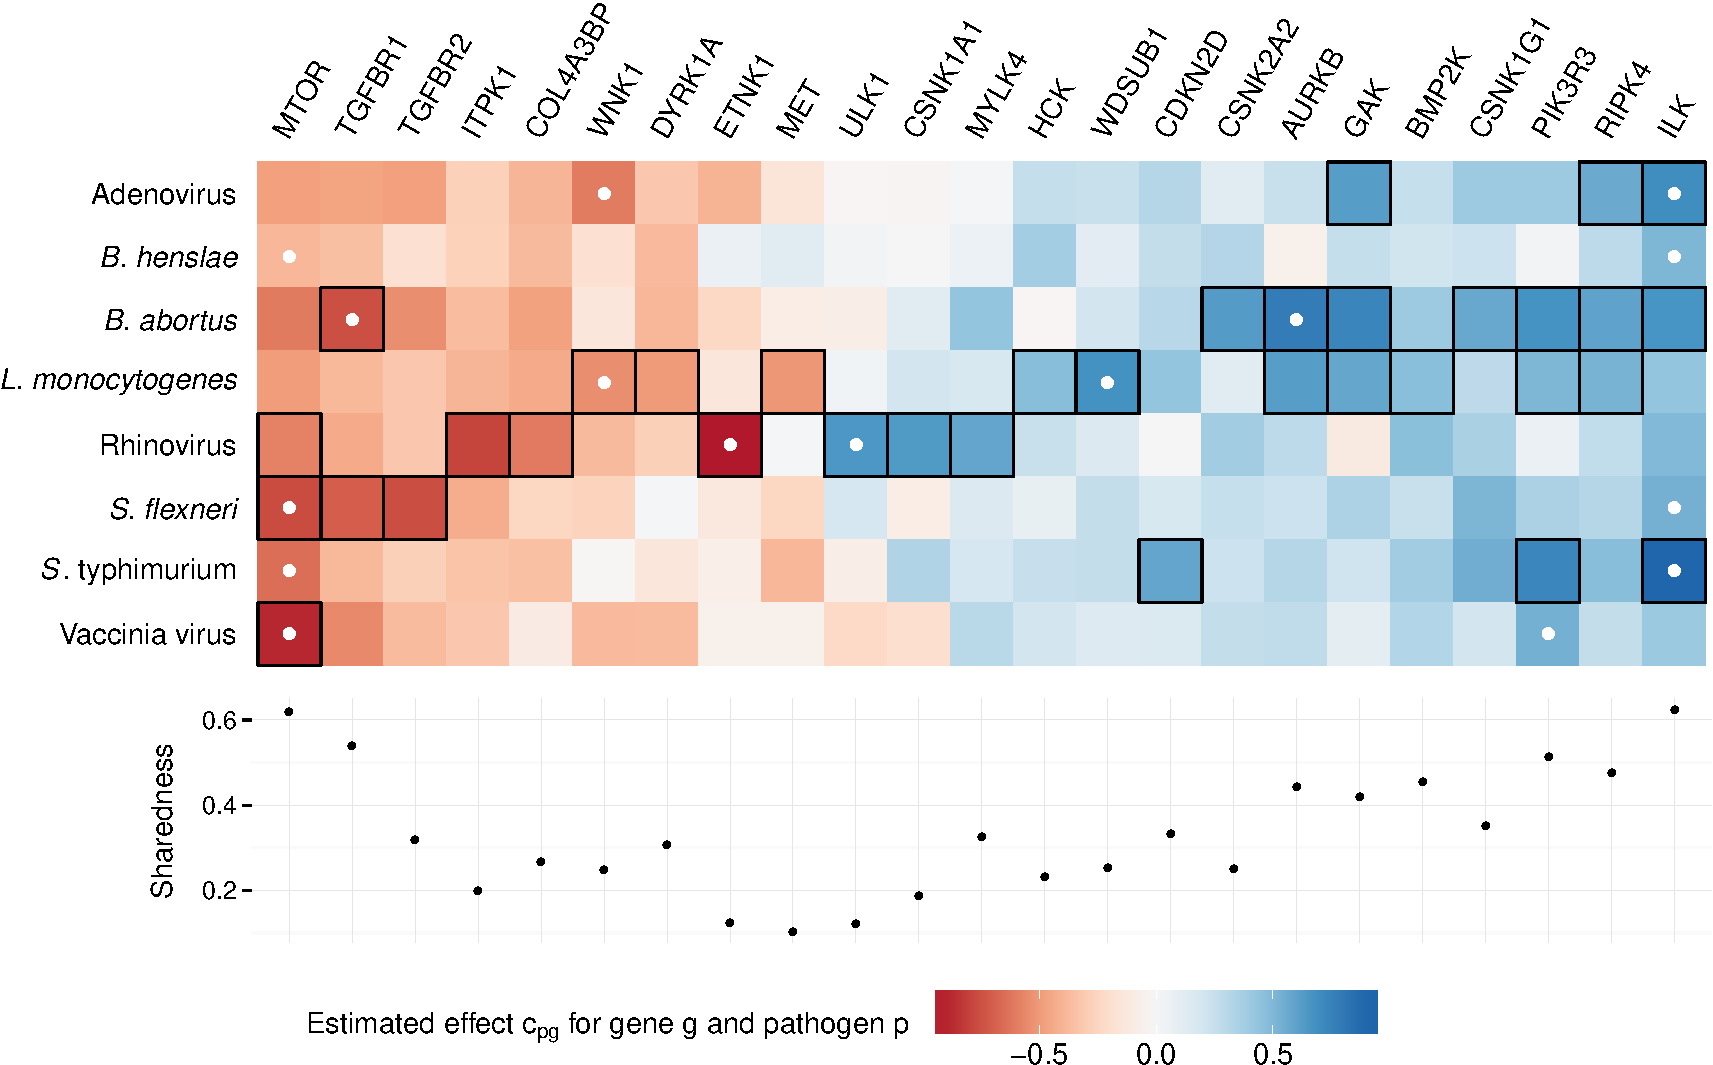
\includegraphics[width=.95\linewidth]{figures/R/pmm-pmm-heatmap-1} 

}

\caption[Heatmap plot showing significant genes for InfectX kinome screens as determined by pmm.]{A heatmap plot as produced by the Bioconductor package pmm, which displays all genes that were determined to be significant hits (FDR < 4; indicated by black borders) for at least one pathogen. Genes are ordered by average c\textunderscript{pg} values and both extrema are marked with white dots, while the sharedness score is shown as a scatterplot below. All available kinome screens were taken into consideration.}\label{fig:pmm-heatmap}
\end{figure}


\end{knitrout}




\begin{equation}
  \fdr(c_{pg}) = q_{pg} = \frac{\pi_0 f_0(c_{pg})}{f(c_{pg})}
\end{equation}

and represents the probability that the effect for a given gene and pathogen is a false discovery. Figure \ref{fig:pmm-heatmap} displays a visualization obtained by applying the PMM package (available on Bioconductor) to kinome-wide InfectX screens. Color-coding corresponds to estimated $c_{pg}$ effects and columns are sorted according to descending mean values. Only genes are included where the estimated \cgls{fdr} is below 0.4 for at least one pathogen (indicated by black borders), suggesting that up to 40\% of individual hits may be superfluous. Centered white dots indicate the maximum and minimum $c_{pg}$ value for each pathogen. For each gene, a sharedness score is displayed as well. This quantity is defined as

\begin{equation}
  s_g = \frac{1}{2} \left(\left(1-\frac{1}{P}\sum_{p=1}^P q_{pg}\right) + \frac{\sum_{p=1}^P \mathds{1}_{q_{pg} < 1}}{P}\right)
\end{equation}

and quantifies how common a hit gene is among pathogens by describing both the extent of downward shift from 1 of the mean $q_{pg}$ value (over all $P=8$ pathogens), as well as the fraction of pathogens that contribute $q_{pg} < 1$ instances.

\section{Preliminary Findings}
Due to the high degree of redundancy in feature extraction during image analysis, a significant amount of correlation among features can be expected. Measurements of objects describing similar image segments, as well as features that build on related concepts, such as mean, median or integrated intensities, will obviously yield similar values and cause a dependence structure that has to be dealt with in statistical analysis. Figure \ref{fig:analysis-correlation} visualizes the issue by showing a heatmap representation of a correlation matrix, obtained from all available \textit{AreaShape}, \textit{Intensity} and \textit{Texture} features for a \textit{Brucella} plate using Dharmacon \cgls{sirna} (J110-2D) and a randomly sampled subpopulation of cells (10\%).

The three feature groups can easily be spotted as diagonal blocks with high within group and lower between group correlation, and the situation is worst for intensity features due to the extensive set of measurements quantifying similar properties (see figure \ref{fig:intensity-features}). The texture segment is subdivided into four groups, corresponding from bottom left to top right to \textit{Cells}, \textit{Nuclei}, \textit{PeriNuclei} and \textit{VoronoiCells}. Absent off-diagonal correlation between nuclear and perinuclear regions is due to mutual exclusivity, whereas the off-diagonal correlation of cell and Voronoi cell features is due to significant overlap.

\begin{knitrout}
\definecolor{shadecolor}{rgb}{0.969, 0.969, 0.969}\color{fgcolor}\begin{figure}

{\centering 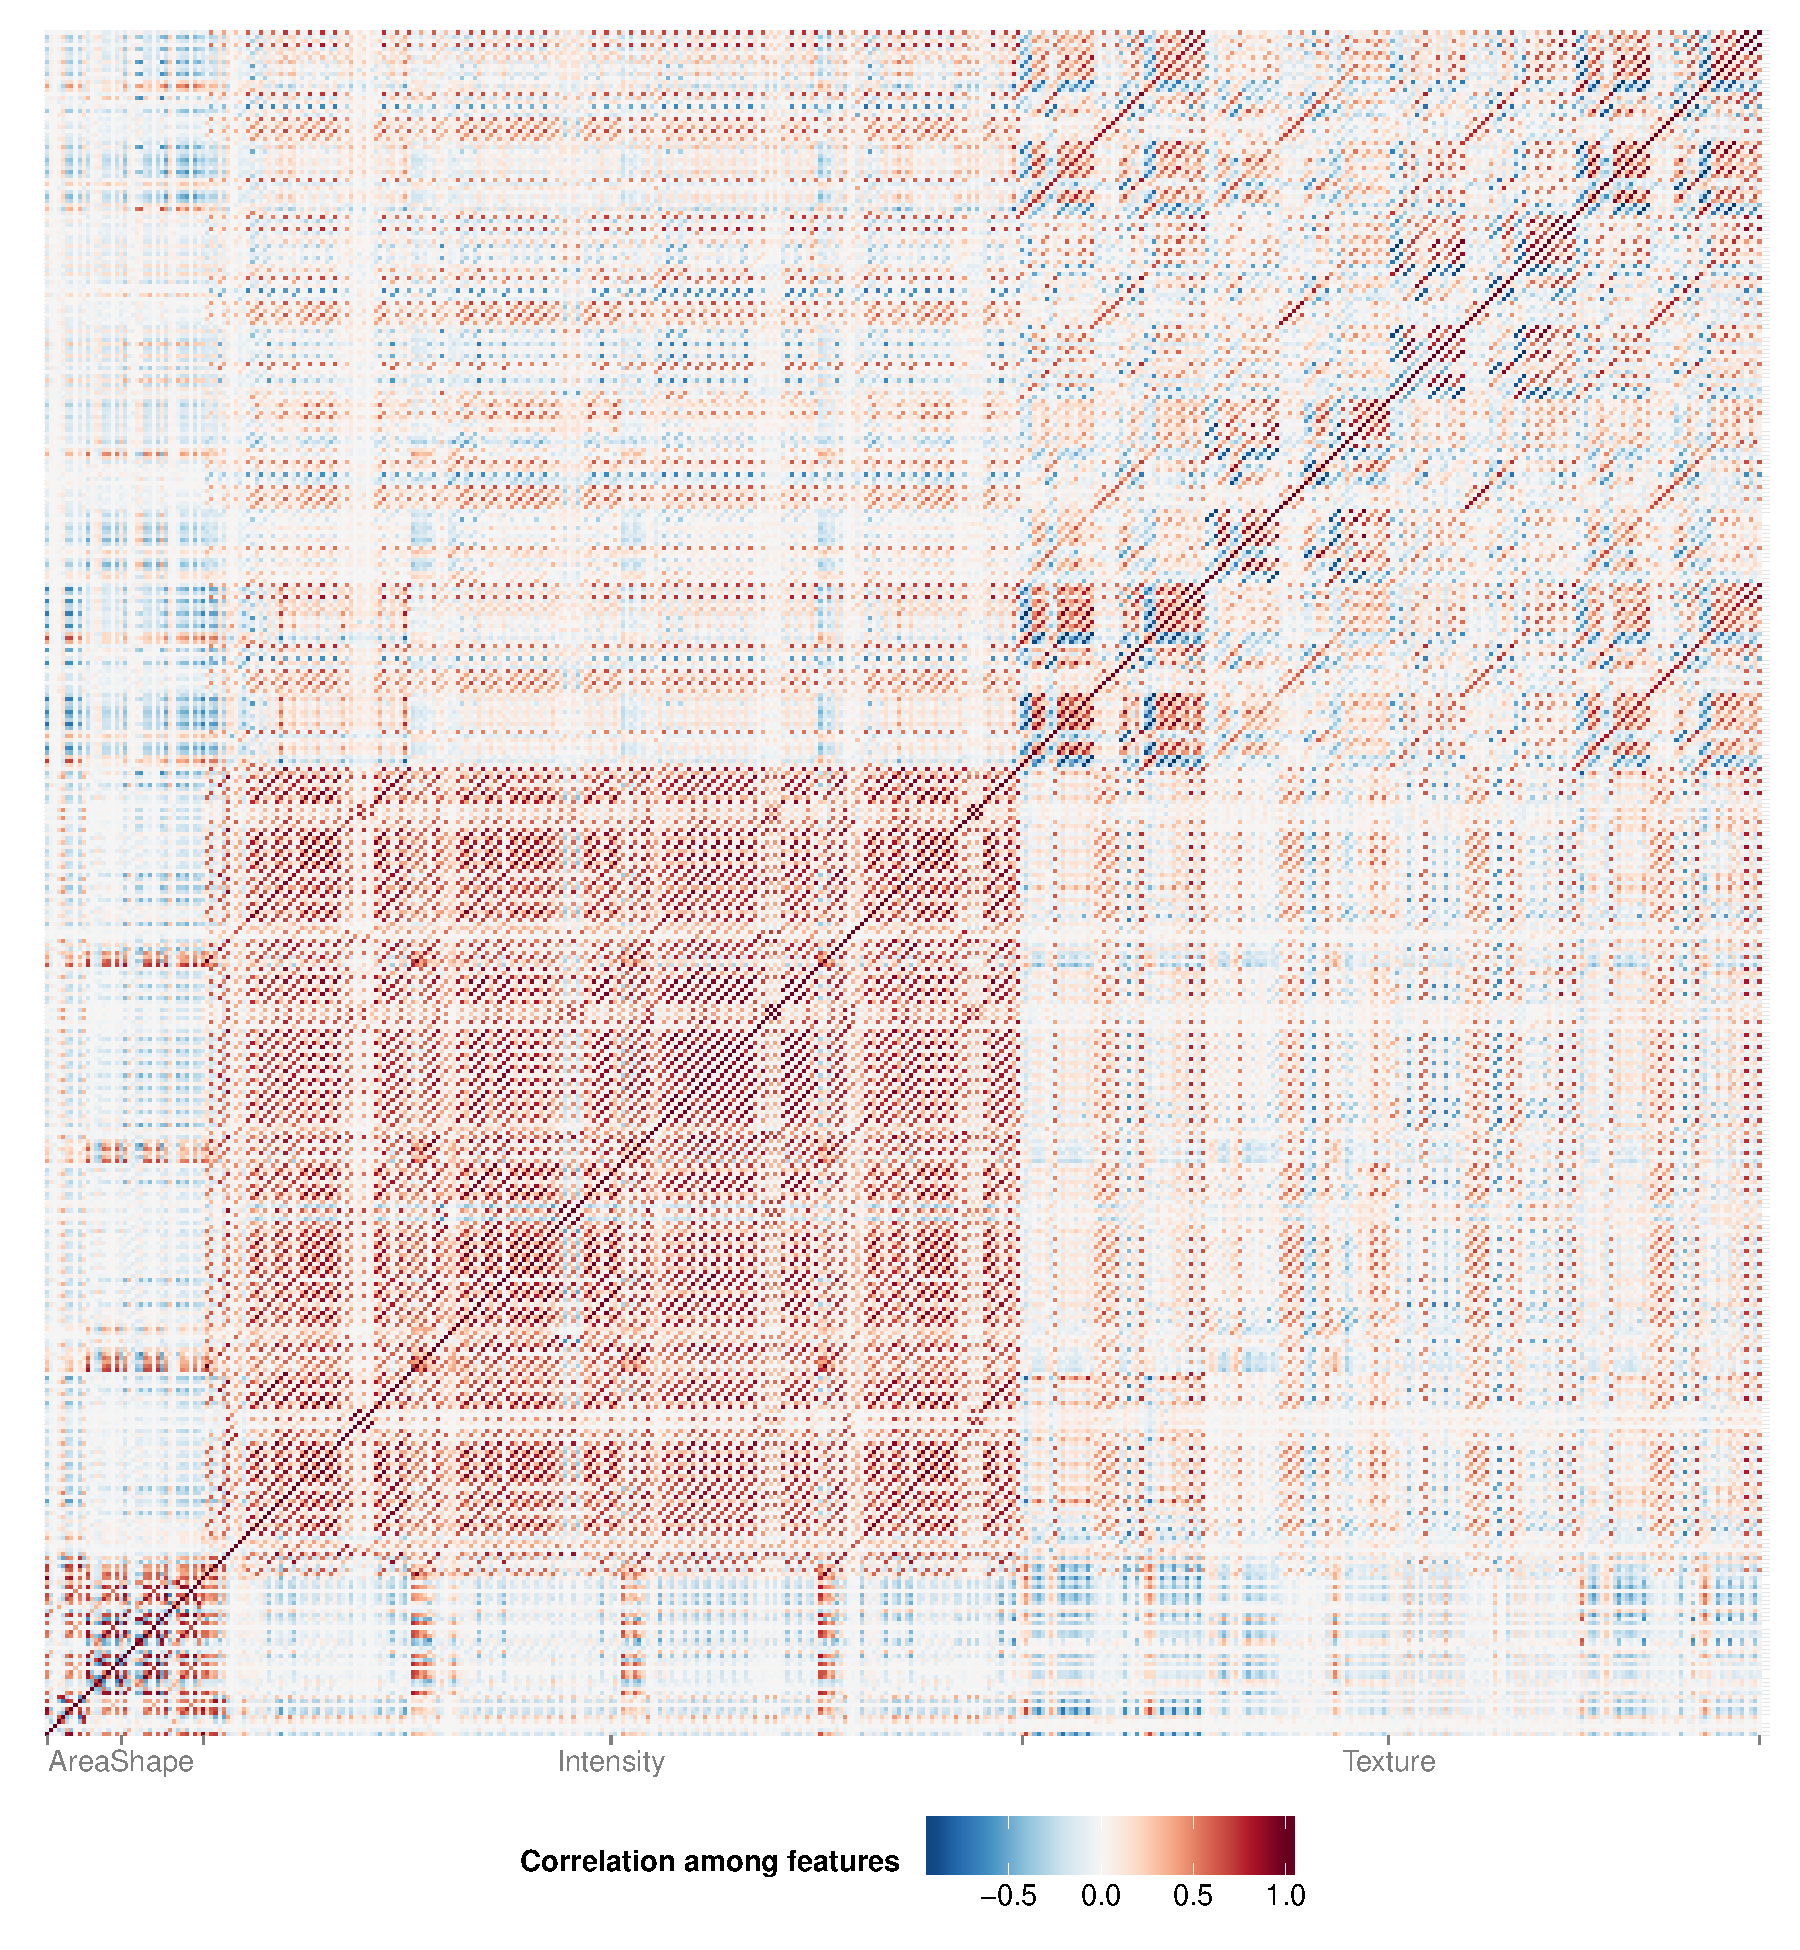
\includegraphics[width=\maxwidth]{figures/R/correlation-heatmap-analysis-correlation-1} 

}

\caption[Heatmap representation of correlation among single cell features.]{A heatmap representation of the correlation matrix obtained by sampling 10\% of single cell feature data available for plate J110-2D illustrates severe correlation among many features that is typical for all datasets. This comes as no surprise due to the redundancy in measured features. The three diagonal blocks correspond to three groups of features, \textit{AreaShape}, \textit{Intensity} and \textit{Texture}.}\label{fig:analysis-correlation}
\end{figure}


\end{knitrout}



In order to deal with this data issue, features are transformed to the coordinate system of \cglspl{pc} prior to \cgls{glm} model fitting. When employing \cgls{pca}, typically the first 10\% (or 30--50) of \cglspl{pc} capture around 90\% of the overall variance in the data, corroborating the above claim of significant correlation among feature vectors. A further problem that is present in many datasets is that pairs of wells can be perfectly separated. This causes problems in maximum likelihood estimation, as affected coefficients are allowed to grow arbitrarily large, but is not unexpected given the large design space. \cGls{pca} provides a tool for addressing the issue by encouraging only inclusion of a subset of \cglspl{pc} and thus reducing dimensionality.

Several \cgls{glm} model fits, based on principal component regression are summarized in table \ref{tab:glm-1}. For the same plate is used in figure \ref{fig:analysis-correlation} (J110-2D, \textit{Brucella}, Dharmacon unpooled, replicate 1), well pairs corresponding to the genes identified by \cgls{pmm} as down-hits, \ACRshort{mtor} (H6) and \ACRshort{pik3r3} (K8), as well as up-hits, \ACRshort{ripk4} (G17) and \ACRshort{tgfbr1} (M4), are formed with all available scrambled wells of the given plate. In order to establish a baseline of sorts, scrambled wells are also paired with each other.

For describing how well the discrepancy between the two input wells is captured, some model characteristics, alongside scores for predictions, are reported. The AIC is a goodness of fit estimate, constituting of the maximized log-likelihood $l$, as well as a penalty term for model size $k$, and is defined as

\begin{equation}
  \aic = 2k - 2l(\Hpi; y).
\end{equation}

Deviance values require caution when interpreted as a goodness-of-fit criterion, especially when used as an absolute measure, rather than being employed in a comparative capacity for nested models (analysis of deviance). The glm function of the R stats package reports both null deviance, defined as

\begin{equation}
  D^{(0)}(y; \pi^{(0)}) = 2l(\widetilde{\pi}; y) - 2l(\pi^{(0)}; y),
\end{equation}

and residual deviance as

\begin{equation}
  D(y; \Hpi) = 2l(\widetilde{\pi}; y) - 2l(\Hpi; y).
\end{equation}

The saturated model $\widetilde{\pi}$ contains as many parameters as there are data observations ($n$) and consequently represents the maximally possible likelihood. The null model $\pi^{(0)}$ contains only an intercept term (i.e. $y = constant$), while the proposed model $\Hpi$ attempts to explain the data using $p+1$ parameters (one for each covariate and an intercept). Finally, the values reported in table \ref{tab:glm-1} as $\Delta\textsubscript{deviance}$ are obtained as

\begin{equation}
  \Delta\textsubscript{deviance} = D^{(0)}(y; \pi^{(0)}) - D(y; \Hpi),
\end{equation}

therefore describing the difference between the quality of fit of the null model to that of the estimated model. Similarly, for the degrees of freedom, 

\begin{equation}
  \Delta\textsubscript{df} = \text{df}_\text{null} - \text{df}_\text{res} = n-1 -(n-(p+1)) = p.
\end{equation}

Under certain assumptions,\footnote{Deviance is only distributed as $\chi^2$ in the limit where for each $i \in \{1, 2, \dotsc, n\}$, the number of identical covariate rows $x_i$ grows to infinity. For continuous regressors, this is typically not the case, as the number of unique $x_i$ will often be very close to $n$. In case of binomially distributed response, the possibility of over-dispersion causes additional issues, which are not further described, as this does not apply to the current situation. Nevertheless, \citeauthor{Nelder1972} state that ``[t]he $\chi^2$ approximation is usually quite accurate for differences of deviances even though it is inaccurate for the deviances themselves.''} $\Delta\textsubscript{deviance} \mathbin{\sim} \chi^2_p$, and therefore a p-value for the significance of the model fit can be calculated. This is not reproduced, as all fits provide highly significant evidence against the null hypothesis, which assumes the fitted model to be no better than the null model.

\renewcommand{\arraystretch}{1.5}
\setlength{\tabcolsep}{0.25em}
\begin{table}
  \centering
  \caption[\cGls{glm} model summaries based on principal components for several well pairings.]{Summaries of several \cgls{glm} models obtained by pairing wells corresponding to the genes \ACRshort{mtor} (H6), \ACRshort{pik3r3} (K8), \ACRshort{ripk4} (G17) and \ACRshort{tgfbr1} (M4) with all available scrambled wells on the same plate (J110-2D). Comparisons among scrambled wells serve as baseline (the scrambled row corresponds to well G1). Model fit is summarized by \cgls{aic}, the difference in deviance and degrees of freedom (both between null and fitted models), as well as prediction scores. The following models suffer from separated data: \ACRshort{mtor} (A24, G1, J2), \ACRshort{pik3r3} (E24, G1, G23, H2, L23), \ACRshort{ripk4} (E2, G23, H2, J2, L1) and Scrambled (A24, G23, H24, J24, L23).}
  \label{tab:glm-1}
  \footnotesize
  \vspace{5px}
  \begin{tabular}{llcccccccccccc}

 &  & A2 & A24 & E2 & E24 & G1 & G23 & H2 & H24 & J2 & J24 & L1 & \multicolumn{1}{c}{L23} \\ 
\hline
\nopagebreak MTOR & \nopagebreak AIC  & \multicolumn{1}{r}{1492} & \multicolumn{1}{r}{3251} & \multicolumn{1}{r}{1601} & \multicolumn{1}{r}{3140} & \multicolumn{1}{r}{1406} & \multicolumn{1}{r}{3541} & \multicolumn{1}{r}{1578} & \multicolumn{1}{r}{3139} & \multicolumn{1}{r}{1484} & \multicolumn{1}{r}{3213} & \multicolumn{1}{r}{1698} & \multicolumn{1}{r}{3781} \\
 & \nopagebreak \textDelta\textsubscript{deviance}  & \multicolumn{1}{r}{3343} & \multicolumn{1}{r}{1734} & \multicolumn{1}{r}{3205} & \multicolumn{1}{r}{2249} & \multicolumn{1}{r}{3552} & \multicolumn{1}{r}{1431} & \multicolumn{1}{r}{2785} & \multicolumn{1}{r}{1756} & \multicolumn{1}{r}{3436} & \multicolumn{1}{r}{1562} & \multicolumn{1}{r}{3152} & \multicolumn{1}{r}{1377} \\
 & \nopagebreak \textDelta\textsubscript{df}  & \multicolumn{1}{r}{46} & \multicolumn{1}{r}{48} & \multicolumn{1}{r}{48} & \multicolumn{1}{r}{47} & \multicolumn{1}{r}{46} & \multicolumn{1}{r}{48} & \multicolumn{1}{r}{48} & \multicolumn{1}{r}{48} & \multicolumn{1}{r}{48} & \multicolumn{1}{r}{48} & \multicolumn{1}{r}{47} & \multicolumn{1}{r}{48} \\
 & \rule{0pt}{1.7\normalbaselineskip}Accuracy  & \multicolumn{1}{r}{0.93} & \multicolumn{1}{r}{0.78} & \multicolumn{1}{r}{0.91} & \multicolumn{1}{r}{0.79} & \multicolumn{1}{r}{0.91} & \multicolumn{1}{r}{0.75} & \multicolumn{1}{r}{0.9} & \multicolumn{1}{r}{0.78} & \multicolumn{1}{r}{0.93} & \multicolumn{1}{r}{0.78} & \multicolumn{1}{r}{0.89} & \multicolumn{1}{r}{0.78} \\
 & \nopagebreak MCC  & \multicolumn{1}{r}{0.86} & \multicolumn{1}{r}{0.55} & \multicolumn{1}{r}{0.82} & \multicolumn{1}{r}{0.56} & \multicolumn{1}{r}{0.83} & \multicolumn{1}{r}{0.49} & \multicolumn{1}{r}{0.8} & \multicolumn{1}{r}{0.55} & \multicolumn{1}{r}{0.86} & \multicolumn{1}{r}{0.56} & \multicolumn{1}{r}{0.78} & \multicolumn{1}{r}{0.56} \\
\rule{0pt}{1.7\normalbaselineskip}PIK3R3 & \nopagebreak AIC  & \multicolumn{1}{r}{4471} & \multicolumn{1}{r}{4280} & \multicolumn{1}{r}{4075} & \multicolumn{1}{r}{4954} & \multicolumn{1}{r}{3509} & \multicolumn{1}{r}{3742} & \multicolumn{1}{r}{3401} & \multicolumn{1}{r}{4396} & \multicolumn{1}{r}{3779} & \multicolumn{1}{r}{3212} & \multicolumn{1}{r}{4170} & \multicolumn{1}{r}{3214} \\
 & \nopagebreak \textDelta\textsubscript{deviance}  & \multicolumn{1}{r}{882} & \multicolumn{1}{r}{1245} & \multicolumn{1}{r}{1244} & \multicolumn{1}{r}{1044} & \multicolumn{1}{r}{1990} & \multicolumn{1}{r}{1769} & \multicolumn{1}{r}{1404} & \multicolumn{1}{r}{1025} & \multicolumn{1}{r}{1672} & \multicolumn{1}{r}{2068} & \multicolumn{1}{r}{1200} & \multicolumn{1}{r}{2512} \\
 & \nopagebreak \textDelta\textsubscript{df}  & \multicolumn{1}{r}{48} & \multicolumn{1}{r}{49} & \multicolumn{1}{r}{50} & \multicolumn{1}{r}{49} & \multicolumn{1}{r}{49} & \multicolumn{1}{r}{49} & \multicolumn{1}{r}{49} & \multicolumn{1}{r}{49} & \multicolumn{1}{r}{50} & \multicolumn{1}{r}{49} & \multicolumn{1}{r}{49} & \multicolumn{1}{r}{49} \\
 & \rule{0pt}{1.7\normalbaselineskip}Accuracy  & \multicolumn{1}{r}{0.71} & \multicolumn{1}{r}{0.71} & \multicolumn{1}{r}{0.76} & \multicolumn{1}{r}{0.69} & \multicolumn{1}{r}{0.77} & \multicolumn{1}{r}{0.8} & \multicolumn{1}{r}{0.74} & \multicolumn{1}{r}{0.75} & \multicolumn{1}{r}{0.77} & \multicolumn{1}{r}{0.81} & \multicolumn{1}{r}{0.7} & \multicolumn{1}{r}{0.84} \\
 & \nopagebreak MCC  & \multicolumn{1}{r}{0.41} & \multicolumn{1}{r}{0.42} & \multicolumn{1}{r}{0.51} & \multicolumn{1}{r}{0.38} & \multicolumn{1}{r}{0.54} & \multicolumn{1}{r}{0.6} & \multicolumn{1}{r}{0.47} & \multicolumn{1}{r}{0.49} & \multicolumn{1}{r}{0.55} & \multicolumn{1}{r}{0.63} & \multicolumn{1}{r}{0.4} & \multicolumn{1}{r}{0.67} \\
\rule{0pt}{1.7\normalbaselineskip}RIPK4 & \nopagebreak AIC  & \multicolumn{1}{r}{4064} & \multicolumn{1}{r}{5554} & \multicolumn{1}{r}{3596} & \multicolumn{1}{r}{6047} & \multicolumn{1}{r}{3076} & \multicolumn{1}{r}{4918} & \multicolumn{1}{r}{3161} & \multicolumn{1}{r}{5055} & \multicolumn{1}{r}{3366} & \multicolumn{1}{r}{4580} & \multicolumn{1}{r}{4094} & \multicolumn{1}{r}{4731} \\
 & \nopagebreak \textDelta\textsubscript{deviance}  & \multicolumn{1}{r}{1751} & \multicolumn{1}{r}{455} & \multicolumn{1}{r}{2179} & \multicolumn{1}{r}{498} & \multicolumn{1}{r}{2900} & \multicolumn{1}{r}{1075} & \multicolumn{1}{r}{2037} & \multicolumn{1}{r}{837} & \multicolumn{1}{r}{2560} & \multicolumn{1}{r}{1153} & \multicolumn{1}{r}{1740} & \multicolumn{1}{r}{1506} \\
 & \nopagebreak \textDelta\textsubscript{df}  & \multicolumn{1}{r}{48} & \multicolumn{1}{r}{49} & \multicolumn{1}{r}{49} & \multicolumn{1}{r}{49} & \multicolumn{1}{r}{48} & \multicolumn{1}{r}{49} & \multicolumn{1}{r}{49} & \multicolumn{1}{r}{49} & \multicolumn{1}{r}{50} & \multicolumn{1}{r}{49} & \multicolumn{1}{r}{49} & \multicolumn{1}{r}{49} \\
 & \rule{0pt}{1.7\normalbaselineskip}Accuracy  & \multicolumn{1}{r}{0.81} & \multicolumn{1}{r}{0.65} & \multicolumn{1}{r}{0.81} & \multicolumn{1}{r}{0.61} & \multicolumn{1}{r}{0.85} & \multicolumn{1}{r}{0.72} & \multicolumn{1}{r}{0.82} & \multicolumn{1}{r}{0.64} & \multicolumn{1}{r}{0.84} & \multicolumn{1}{r}{0.71} & \multicolumn{1}{r}{0.79} & \multicolumn{1}{r}{0.74} \\
 & \nopagebreak MCC  & \multicolumn{1}{r}{0.61} & \multicolumn{1}{r}{0.29} & \multicolumn{1}{r}{0.61} & \multicolumn{1}{r}{0.22} & \multicolumn{1}{r}{0.7} & \multicolumn{1}{r}{0.44} & \multicolumn{1}{r}{0.62} & \multicolumn{1}{r}{0.27} & \multicolumn{1}{r}{0.67} & \multicolumn{1}{r}{0.42} & \multicolumn{1}{r}{0.57} & \multicolumn{1}{r}{0.48} \\
\rule{0pt}{1.7\normalbaselineskip}Scrambled & \nopagebreak AIC  & \multicolumn{1}{r}{4673} & \multicolumn{1}{r}{2480} & \multicolumn{1}{r}{4366} & \multicolumn{1}{r}{2843} & \multicolumn{1}{c}{--} & \multicolumn{1}{r}{2130} & \multicolumn{1}{r}{3731} & \multicolumn{1}{r}{2800} & \multicolumn{1}{r}{4673} & \multicolumn{1}{r}{1651} & \multicolumn{1}{r}{4670} & \multicolumn{1}{r}{1885} \\
 & \nopagebreak \textDelta\textsubscript{deviance}  & \multicolumn{1}{r}{670} & \multicolumn{1}{r}{3032} & \multicolumn{1}{r}{941} & \multicolumn{1}{r}{3140} & \multicolumn{1}{c}{--} & \multicolumn{1}{r}{3368} & \multicolumn{1}{r}{1065} & \multicolumn{1}{r}{2610} & \multicolumn{1}{r}{765} & \multicolumn{1}{r}{3615} & \multicolumn{1}{r}{687} & \multicolumn{1}{r}{3827} \\
 & \nopagebreak \textDelta\textsubscript{df}  & \multicolumn{1}{r}{48} & \multicolumn{1}{r}{48} & \multicolumn{1}{r}{49} & \multicolumn{1}{r}{48} & \multicolumn{1}{c}{--} & \multicolumn{1}{r}{48} & \multicolumn{1}{r}{49} & \multicolumn{1}{r}{49} & \multicolumn{1}{r}{49} & \multicolumn{1}{r}{47} & \multicolumn{1}{r}{48} & \multicolumn{1}{r}{48} \\
 & \rule{0pt}{1.7\normalbaselineskip}Accuracy  & \multicolumn{1}{r}{0.69} & \multicolumn{1}{r}{0.89} & \multicolumn{1}{r}{0.69} & \multicolumn{1}{r}{0.86} & \multicolumn{1}{c}{--} & \multicolumn{1}{r}{0.88} & \multicolumn{1}{r}{0.74} & \multicolumn{1}{r}{0.85} & \multicolumn{1}{r}{0.7} & \multicolumn{1}{r}{0.92} & \multicolumn{1}{r}{0.65} & \multicolumn{1}{r}{0.9} \\
 & \nopagebreak MCC  & \multicolumn{1}{r}{0.38} & \multicolumn{1}{r}{0.77} & \multicolumn{1}{r}{0.39} & \multicolumn{1}{r}{0.73} & \multicolumn{1}{c}{--} & \multicolumn{1}{r}{0.76} & \multicolumn{1}{r}{0.46} & \multicolumn{1}{r}{0.7} & \multicolumn{1}{r}{0.4} & \multicolumn{1}{r}{0.83} & \multicolumn{1}{r}{0.31} & \multicolumn{1}{r}{0.81} \\
\rule{0pt}{1.7\normalbaselineskip}TGFBR1 & \nopagebreak AIC  & \multicolumn{1}{r}{3897} & \multicolumn{1}{r}{4968} & \multicolumn{1}{r}{3807} & \multicolumn{1}{r}{5529} & \multicolumn{1}{r}{3683} & \multicolumn{1}{r}{4825} & \multicolumn{1}{r}{3244} & \multicolumn{1}{r}{4969} & \multicolumn{1}{r}{3589} & \multicolumn{1}{r}{3887} & \multicolumn{1}{r}{4335} & \multicolumn{1}{r}{4722} \\
 & \nopagebreak \textDelta\textsubscript{deviance}  & \multicolumn{1}{r}{2018} & \multicolumn{1}{r}{1147} & \multicolumn{1}{r}{2069} & \multicolumn{1}{r}{1135} & \multicolumn{1}{r}{2400} & \multicolumn{1}{r}{1273} & \multicolumn{1}{r}{2040} & \multicolumn{1}{r}{1025} & \multicolumn{1}{r}{2439} & \multicolumn{1}{r}{1944} & \multicolumn{1}{r}{1599} & \multicolumn{1}{r}{1626} \\
 & \nopagebreak \textDelta\textsubscript{df}  & \multicolumn{1}{r}{47} & \multicolumn{1}{r}{48} & \multicolumn{1}{r}{49} & \multicolumn{1}{r}{48} & \multicolumn{1}{r}{48} & \multicolumn{1}{r}{48} & \multicolumn{1}{r}{49} & \multicolumn{1}{r}{48} & \multicolumn{1}{r}{49} & \multicolumn{1}{r}{48} & \multicolumn{1}{r}{48} & \multicolumn{1}{r}{48} \\
 & \rule{0pt}{1.7\normalbaselineskip}Accuracy  & \multicolumn{1}{r}{0.81} & \multicolumn{1}{r}{0.71} & \multicolumn{1}{r}{0.8} & \multicolumn{1}{r}{0.69} & \multicolumn{1}{r}{0.81} & \multicolumn{1}{r}{0.71} & \multicolumn{1}{r}{0.8} & \multicolumn{1}{r}{0.7} & \multicolumn{1}{r}{0.85} & \multicolumn{1}{r}{0.8} & \multicolumn{1}{r}{0.77} & \multicolumn{1}{r}{0.77} \\
 & \nopagebreak MCC  & \multicolumn{1}{r}{0.6} & \multicolumn{1}{r}{0.41} & \multicolumn{1}{r}{0.6} & \multicolumn{1}{r}{0.39} & \multicolumn{1}{r}{0.62} & \multicolumn{1}{r}{0.42} & \multicolumn{1}{r}{0.57} & \multicolumn{1}{r}{0.38} & \multicolumn{1}{r}{0.69} & \multicolumn{1}{r}{0.59} & \multicolumn{1}{r}{0.53} & \multicolumn{1}{r}{0.53} \\
\hline 
\end{tabular}


%\newcommand{\knitrDataGlm1PerSepScram}{pasteAnd(names(perfect.sep$Scrambled)[which(perfect.sep$Scrambled)])}
%\newcommand{\knitrDataGlm1PerSepMtor}{pasteAnd(names(perfect.sep$MTOR)[which(perfect.sep$MTOR)])}
%\newcommand{\knitrDataGlm1PerSepTgfbr1}{pasteAnd(names(perfect.sep$TGFBR1)[which(perfect.sep$TGFBR1)])}
%\newcommand{\knitrDataGlm1PerSepRipk4}{pasteAnd(names(perfect.sep$RIPK4)[which(perfect.sep$RIPK4)])}
%\newcommand{\knitrDataGlm1PerSepPik3r3}{pasteAnd(names(perfect.sep$PIK3R3)[which(perfect.sep$PIK3R3)])}

\end{table}

Moving along to prediction scores, table \ref{tab:glm-1} shows both accuracy and \cgls{mcc} values obtained by separating 20\% of data for each group from training data and evaluating predictions using test data. Accuracy is defined as

\begin{equation}
  \text{Acc} = \frac{n_{tp} + n_{tn}}{n_p+n_n}
\end{equation}

where $n_{tp}$ represents the number of true positives, $n_{tn}$ the count of true negatives and $p$, $n$ the number of positive and negative instances, respectively. The \acrshort{mcc} \citep{Matthews1975} can be evaluated as

\begin{equation}
  \text{Mcc} = \frac{n_{tp} n_{tn} - n_{fp} n_{fn}}{\sqrt{(n_{tp} + n_{fp})(n_{tp} + n_{fn})(n_{tn} + n_{fp})(n_{tn} + n_{fn})}}
\end{equation}

and $n_{fp}$, $n_{fn}$ correspond to false positives and false negatives. Values for \cgls{mcc} range from $-1$ (total disagreement) to $1$ (perfect prediction), and the midpoint $0$ indicates random prediction.

Given these model characteristics, two patterns emerge: (1) the ability to distinguish two wells is dependent on well distance within the plate and (2) the differences among scrambled wells, in terms of computed quality of fit estimates, are comparable to those that are observed when modeling the discrepancy between hit genes and control wells. To make the first claim, well locations are required: \ACRshort{mtor} (H6), \ACRshort{pik3r3} (K8), \ACRshort{ripk4} (G17), \ACRshort{tgfbr1} (M4) and Scrambled (A2, A24, E2, E24, G1, G23, H2, H24, J2, J24, L1 and L23). For both \ACRshort{mtor} and \ACRshort{tgfbr1}, which represent early-row, down-hit genes, an alternating sequence is clearly discernible and is characterized by lower AIC, larger $\Delta\textsubscript{deviance}$ and better predictive power for wells that are closer together, while the opposite holds for comparisons among scrambled wells. The effect is less distinct for \ACRshort{pik3r3} and \ACRshort{ripk4} which both are located more towards the plate center and are identified as up-hits. For \ACRshort{ripk4} the alternations are still noticeable albeit, as in scrambled, polarity is reversed. This is indicative of some technical artifacts contained in the data, that dominate biological features of interest. Furthermore, the excellent predictions that can be made based on membership to either one of a scrambled well pair is disconcerting, as biologically they should be equivalent. Again, technical effects seemingly dominate.

In 18 of the 59 models displayed in table \ref{tab:glm-1}, a warning regarding perfectly separated data is issued by the glm routine (in the example of \ACRshort{mtor}, wells A24, G1 and J2). For this particular case, the matter is not further investigated, as it does not have obviously relevant consequences.\footnote{For other inquiries, not reported here, perfect separation was addressed by reducing the number of \cglspl{pc} or using regularized procedures. Furthermore the issue was studied by solving associated linear programming problems in order to explicitly find the separating hyperplane and thus determine whether this is actually part of the data or caused by numerical shortcomings of the glm implementation. In an example by \citeauthor{Gelman2007} it is shown that a response such as \mintinline{text}{y <- rep (c(1,0),c(10,5))} in a model containing only an intercept, will trigger the separation warning dependent on starting values (i.e. using \mintinline{text}{start=2.6}, glm runs fine, whereas \mintinline{text}{start=2.7} issues the warning). A further effect known to cause problems under certain circumstances, especially for convergence, is the Hauck-Donner phenomenon. As it turns out, separating hyperplanes can reliably be determined, most probably owing in part to the high dimensional setting (with respect to predictor variables).} Affected data points appear in line with well pairs where no complete data separation is possible and the above arguments still hold if possibly questionable data is excluded (albeit patterns are less clearly distinguishable).

Apart from the results shown, many similar investigations were performed, using other datasets and\slash or slightly different methods. Further \textit{Brucella} plates were considered, pooled \cgls{sirna} experiments, libraries from Ambion and Qiagen, as were several \textit{Salmonella} plates and for some inquiries, cell population was limited to infected only. Method-wise, ridge and elastic net penalized regression (glmnet), other glm implementations, such as glm2 (\citet{Marschner2011}; uses a more robust fitting procedure), brglm (\citet{Kosmidis2007}; deals with data separation by penalized maximum likelihood) and bayesglm (\citet{Gelman2007}; regularizes coefficients though a weakly informative prior distribution), as well as step-wise model building (using the step function of the R stats package) was explored.

% bootstrapped stuff

All analysis performed clearly indicates that for the intended type of modeling, an effective normalization scheme has to be developed that is able to capture technical effects (and perhaps even spurious biological artifacts), without destroying phenotypic information coming from gene knockdown and pathogen infection. Attempts of achieving this are outlined in the following section.

\section{Data Normalization}
\label{sec:data-normalization}
The large amount of technical variation, coupled with treating biological systems, which in turn are associated with their own inherent noise, make the analysis of \cgls{hts} data a challenging endeavor, requiring thorough normalization methods. The poor reproducibility that often afflicts \cgls{sirna} experiments may in part be addressed and even resolved with the development of effective corrections that do not negatively affect phenotypes of interest. The following sections outline two types of normalization approaches, plate and well level corrections via Z-scoring\slash B-scoring and using residuals of a \cgls{mars} model at single cell level, as well as the application of such procedures to InfectX datasets.

\subsection{Plate and Well Level Normalization}
In order to correct \cgls{sirna} data for experimental artifacts at plate and well levels, two schemes have become standard practice, Z-scoring and B-scoring \citep{Malo2006}. The former is widely known (outside the field of \cgls{sirna} analysis) and is defined as

\begin{equation}
  z_{ij} = \frac{x_{ij} - \mu_j}{\sigma_j}, \quad i=1, \dotsc, n \enspace \text{and} \enspace j=1, \dotsc, m
\end{equation}

where $n$ is the number of cells, $m$ the number of features and $x_{.j}$ the data vector of feature j to be normalized, while $\mu_j$ represents the sample mean and $\sigma_j$ the sample standard deviation of feature j, as

\begin{equation}
  \mu_j = \frac{1}{n} \sum_{i=1}^n x_{ij} \quad \text{and} \quad \sigma_j = \sqrt{\frac{1}{n-1} \sum_{i=1}^n (x_{ij}-\mu_j)^2}.
\end{equation}

Applying Z-scoring therefore both centers data around zero and scales dispersion to unit variance. B-scoring is more domain specific and deals with row and column effects that have been discussed previously (e.g. pipetting issues, leading to horizontal patterns or temporal effects such as decay of actin stain intensity, resulting in a vertically oriented gradient, when imaging is performed column-wise). B-scoring can be expressed as

\begin{equation}
  b_{rcp} = \frac{\epsilon_{rcp}}{\mad(r)} = \frac{x_{rcp} - (\Hmu_p + \widehat{\alpha}_{rp} + \widehat{\beta}_{cp})}{\mad(r)}, \quad r=1, \dotsc, N \enspace \text{and} \enspace c=1, \dotsc, M,
\end{equation}

where $N$ is the number of plate rows and $M$ the number of plate columns (in the present setup 16 and 24 respectively). Estimates for row and column effects, $\widehat{\alpha}_{rp}$ and $\widehat{\beta}_{cp}$, are obtained by fitting a two-way median polish algorithm. Together with an estimate for plate average $\Hmu_p$, these three parameters are used to determine a residual $\epsilon_{rcp}$, which divided by the \cgls{mad} over the whole plate, yields the B-scored value $b_{rcp}$. Median polishing proceeds by augmenting the plate layout with an additional column and row as

\begin{equation*}
  \begin{array}{cccc|c}
    \epsilon_{1,1,p} & \epsilon_{1,2,p} & \cdots & \epsilon_{1,M,p} & \alpha_{1,p} \\
    \epsilon_{2,1,p} & \epsilon_{2,2,p} & \cdots & \epsilon_{2,M,p} & \alpha_{2,p} \\
    \vdots  & \vdots  & \ddots & \vdots & \vdots \\
    \epsilon_{N,1,p} & \epsilon_{N,2,p} & \cdots & \epsilon_{N,M,p} & \alpha_{N,p} \\
    \hline
    \beta_{1,p} & \beta_{2,p} & \cdots & \beta_{M,p} & \mu_{p} \\
  \end{array}
\end{equation*}

and initializing the values as $\epsilon_{rcp} = x_{rcp}$ and $\alpha_{rp} = \beta_{cp} = \mu_p = 0$. A row sweep consists of iterating all rows, calculating the median of $(\epsilon_{i,1,p}, \epsilon_{i,2,p}, \dotsc, \epsilon_{i,M,p})$ for each row $i$, subtracting the resulting value from $(\epsilon_{i,1,p}, \epsilon_{i,2,p}, \dotsc, \epsilon_{i,M,p})$ and adding it to $\alpha_{i,p}$. The same procedure is also applied to the column effect row where the median of $(\beta_{1,p}, \beta_{2,p}, \dotsc, \beta_{M,p}$ is subtracted from $(\beta_{1,p}, \beta_{2,p}, \dotsc, \beta_{M,p}$ and added to $\mu_p$). A column sweep is carried out analogously and the two procedures are alternated until all rows and columns of residuals have median zero, as do the vectors of row and column effects (or fall below a threshold close to zero). Usually only a couple of sweeps in each direction (\tilde 2) are needed. The results are non-unique as they depend on whether row or column sweeps are put first. Furthermore, using means instead of medians yields a least squares decomposition as in two-way \cgls{anova} without iteration, which is less robust towards outliers \citep{Brown2006,Venables2002}. The \cgls{mad} is defined as

\begin{equation}
  \mad(x) = \median\left(\abs{x_k-\median(x)}\right).
\end{equation}

and therefore provides an estimation of data spread which is more robust towards outliers as other measures of dispersion, such as standard deviation.

While B-scoring has proven to be a capable normalization tool for data coming from a plate reader or phenotypic data like infection scores as generated from InfectX screens, where there is a single value per well to be adjusted for experimental artifacts, the situation for single cell feature data is much more complex. Ideally, Z-scoring and B-scoring are able to correct for issues at plate and well level, but data hierarchy goes beyond that for InfectX datasets. For example, data can be split into images which are captured individually, possibly with different imaging parameters and therefore may require differing treatment.

\subsection{Multivariate Adaptive Regression Splines}
At cellular level of granularity, an abundance of additional sources of noise may directly be addressed. This includes technical issues, as well as biological variability. Examples for the former are location of cell within the well which might be relevant due some degree of curvature of the well bottom, inducing focusing problems towards well borders, or location of cell within image, possibly affecting cellular features due to varying optical properties moving away from the image center (e.g. vignetting, decrease in sharpness, chromatic aberration, etc.). Biological sources of noise are even more plentiful and therefore increasingly harder to address. Obvious targets include general cell state parameters, such as cell cycle stage or whether the cell is apoptotic with the difficulty here being reliably determining these factor variables.

Work by \citeauthor{Snijder2012} elucidates the importance of cellular population context in cell-to-cell variability. In a comprehensive analysis of virally perturbed \cgls{sirna} screens they demonstrate that parameters such as local cell density, population size and cell location within cellular aggregates significantly alter measured phenotypes. Building on these results, \citeauthor{Knapp2011} propose a normalization scheme by fitting a \cgls{mars} model to a selection of features that represent the cellular population context (among other technical parameters) and using only the residuals for further analysis.

\cGls{mars} is an nonparametric regression procedure for finding a piecewise linear solution. No assumptions on data distributions are made and \cgls{mars} represents a capable method for high-dimensional settings with respect to predictor variables. The following short introduction into \cgls{mars} modeling is largely based on \citet{Hastie2009}. Basis functions of the form

\begin{equation}
  (x_j-t)_+ = \max(0, x_j-t) =
  \begin{cases}
    x_j-t,& \text{if } x_j > t\\
    0,              & \text{otherwise},
  \end{cases}
\end{equation}

and $(t-x_j)_+$, which are combined as reflected pairs, are used for describing the model surface. Such linear splines contain a knot at value $t$, separating the function support into a zero part and a nonzero domain, which for the reflected version are swapped with opposite slope. Despite each basis function only depending on a single covariate ($j \in \{1, 2, \dotsc, p\}$), they are considered as functions over the complete predictor space $\R^p$. Model building proceeds by maintaining two sets of reflected pairs, candidates and active pairs, where the active set initially contains only a constant term and candidates include all $2np$ possible functions with knots at each observed value $x_{ij}$

\begin{equation}
  C = \left\{(x_j-t)_+, (t-x_j)_+ \given t\in\{x_{1j}, x_{2j}, \dotsc, x_{nj}, \} \land j\in\{1, 2, \dotsc, p\} \right\}.
\end{equation}

A \cgls{mars} model has the form

\begin{equation}
  g(x) = \mu + \sum_{m=1}^M \beta_m h_m(x),
\end{equation}

where the coefficients $\beta_m$ represent slopes of basis functions $h_m(\cdot)$ which can either be chosen from individual functions in C or by forming products of functions from the set of candidates C and thereby directly model interactions between variables. The active set is initialized with $A=\{h_0(x)=1\}$ and in an iterative procedure, for $k=1, 2, \dotsc, M$, the best pair of functions $\{h_{2k-1}(x), h_{2k}(x)\}$ with respect to the largest reduction in residual sum of squares is chosen and added to the active set, whereby the new additions are products of a reflected pair from the candidate set with a function $h_l(x)$ of the active set

\begin{subequations}
\begin{align}
  h_{2k-1}(x) &= h_l(x) \cdot (x_j-t)_+ \\
  h_{2k}(x) &= h_l(x) \cdot (t-x_j)_+.
\end{align}
\end{subequations}

The $2k$ coefficients are estimated by least squares and in each step the model grows by two basis functions. Termination of the iteration process occurs when a preset number of basis functions have been added to the active set, typically leading to a model that over-fits the data. A pruning scheme follows that from each pair of functions $\{h_{2k-1}(x), h_{2k}(x)\}$, removes the one that yields the smaller increase in residual sum of squares. In order to determine the right amount of backwards elimination and find the best model $\widehat{g}_\lambda^{\ *}(x)$, for each stage, a \cgls{gcv} score is computed for the current model $\widehat{g}_\lambda(x)$. Another possibility is performing cross validation but this is often foregone due to computational expense. The \cgls{gcv} criterion is defined as

\begin{equation}
  \text{gcv}(\lambda) = \frac{1}{n}\frac{\sum_{i=1}^n \left(y_i-\widehat{g}_\lambda(x_i)\right)^2}{\left(1-\frac{C(\lambda)}{n}\right)^2},
\end{equation}

where cost complexity term $C(\lambda)$ represents the effective number of parameters, computed as a sum of the number of linearly independent basis functions with the product of a smoothing parameter $d$ and the total number of terms. The value of $d$ is typically 2 (additive model) or 3 (higher orders allowed) and controls the amount of kinks introduced \citep{Friedman1991}.

By having the option of combining functions in the active set with newly entering terms, the algorithm builds a hierarchical model in the sense that interactions of added variables are only possible if all interacting partners are already present, forming an interaction of one order less. The reasoning behind this is that otherwise the search space would grow exponentially, causing computational issues for higher order interactions and in many cases it seems justifiable to require main effects as basis for interactions. Furthermore, the formation of powers is not allowed as a term may only enter a single time in an iteration, again limiting the search space in favor of computational efficiency. For interpretability and in larger problems for performance reasons, it is often advisable to restrict the number of interactions to degree 2 or 3.

\subsection{Normalization of Single Cell Data}
Implemented as part of singleCellFeatures, are both procedures for applying Z-scoring and B-scoring, as well as fitting a user-defined \cgls{mars} model to each feature selected to be normalized (see section \ref{sec:scf-aug-norm}). Two sets of features so far have been used as predictors in \cgls{mars}, a simpler, more conservative selection intended for targeting technical issues and a larger set based on the work of \citet{Knapp2011}, which includes population context.

\begin{knitrout}
\definecolor{shadecolor}{rgb}{0.969, 0.969, 0.969}\color{fgcolor}\begin{figure}

{\centering 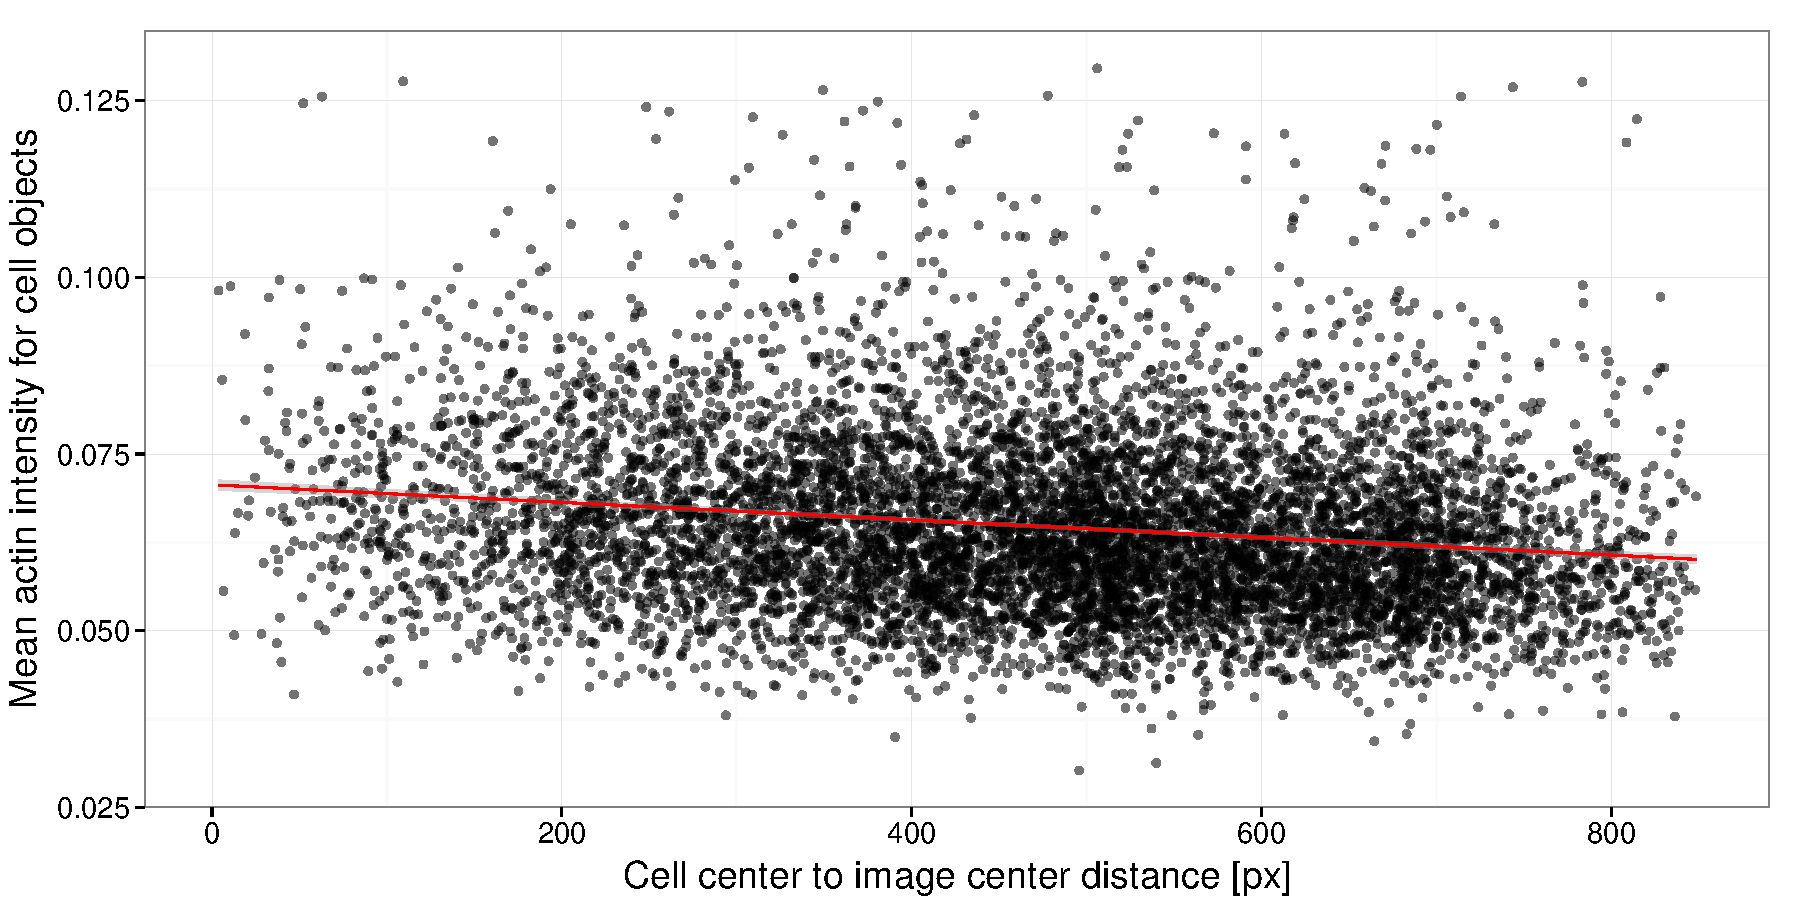
\includegraphics[width=.95\linewidth]{figures/R/location-trends-data-location-trend-1} 

}

\caption[Scatterplot visualization showing mean actin intensity against object distance from image center alongside a trend line.]{In order to illustrate the relationship between object location and feature values, a thinned out scatterplot (only a randomly sampled 1\% of datapoints are shown) of mean actin intensity against distance from image cetner is reproduced alognside a trendline as calculated by gam of the CRAN mgcv package. An approximately linear trend is discernible which can be found in many feature types.}\label{fig:data-location-trend}
\end{figure}


\end{knitrout}


The smaller of the two contains predictors for object location within image and well, in addition to feature specific terms obtained through B-scoring. Motivated by findings as displayed in figure \ref{fig:data-location-trend}, cellular features are normalized using the locations of their respective nuclei. Figure \ref{fig:data-location-trend} shows a scatter-plot of mean actin intensity in cell objects versus their locations measured as Euclidean distance from the image center. The trend line (calculated by the function \mintinline{text}{gam} of the \acrshort{cran} package mgcv) indicates an approximately linear relationship with negative slope. Such dependencies can reliably be found for most features, both at well and image level and their significance can be established by fitting multiple linear regression models. The resulting p-values for an overwhelming majority of features are highly significant, below machine accuracy ($<2\cdot10^{-16}$). As this effect constitutes an entirely experimental artifact, it seems reasonable to correct for location with respect to well and image centers.

Population context normalization additionally includes features for nucleus area, cell count per image, nuclear form factor, cell area, cell density, whether the cell is close to an image border and whether the cell is located at the edge of a colony. \citeauthor{Knapp2011} suggest that the procedure be carried out for a complete screen and while that is not a difficult task for the data they processed (only a single feature, 10-fold fewer cells), it is far more demanding for IndectX data. For an investigation considering only infected cells of a \textit{Brucella}, Dharmacon unpooled screen, this was necessary as only few cells per \ACRshort{mtor} well are available which consequently have to be aggregated.

In order for the \cgls{mars} procedure to even out technical effects, spanning multiple plates, it is, at least for the dataset mentioned above, important to center data with respect to plate means prior to fitting the \cgls{mars} model, as otherwise results are unsatisfactory (neither row, nor column effects can be completely removed, most probably due to underestimated plate effects). A further issue is that of memory. The entire screen consists of $2 \times 12$ plates which would require on the order of \SI{200}{\giga\byte} for storing the data alone, not taking operational overhead into account. This is infeasible, even for large memory machines. As \ACRshort{mtor} wells are located on 8 of the 24 plates, only these were handled jointly.

Computationally, two avenues were explored, keeping all data in memory and utilizing disk scratch to lower the astronomical memory requirements of the former approach. Using a reasonably fast permanent storage device such as a \cgls{ssd}, screen wide normalization is readily possible on regular desktop machines but frequent data fetching from storage incurs a significant time penalty. Processing 8 plates and \tilde 400 features takes on the order of \SI{36}{\hour}. Handling all data in memory speeds up the process to 6--\SI{8}{\hour}, but handling 8 plates, which alone only require \tilde \SI{60}{\giga\byte}, required a complete \SI{256}{\giga\byte} node of the ETH Euler cluster for processing.

Both the exclusively technical normalization procedure and the one including biological features additionally incorporate predictors obtained through B-scoring. For each of the features that are selected, the corresponding row, column and plate effects are calculated and are included with the mars model which consequently contains 5 predictors for the simple and 9 predictors for the more complex variant.

\begin{knitrout}
\definecolor{shadecolor}{rgb}{0.969, 0.969, 0.969}\color{fgcolor}\begin{figure}

{\centering 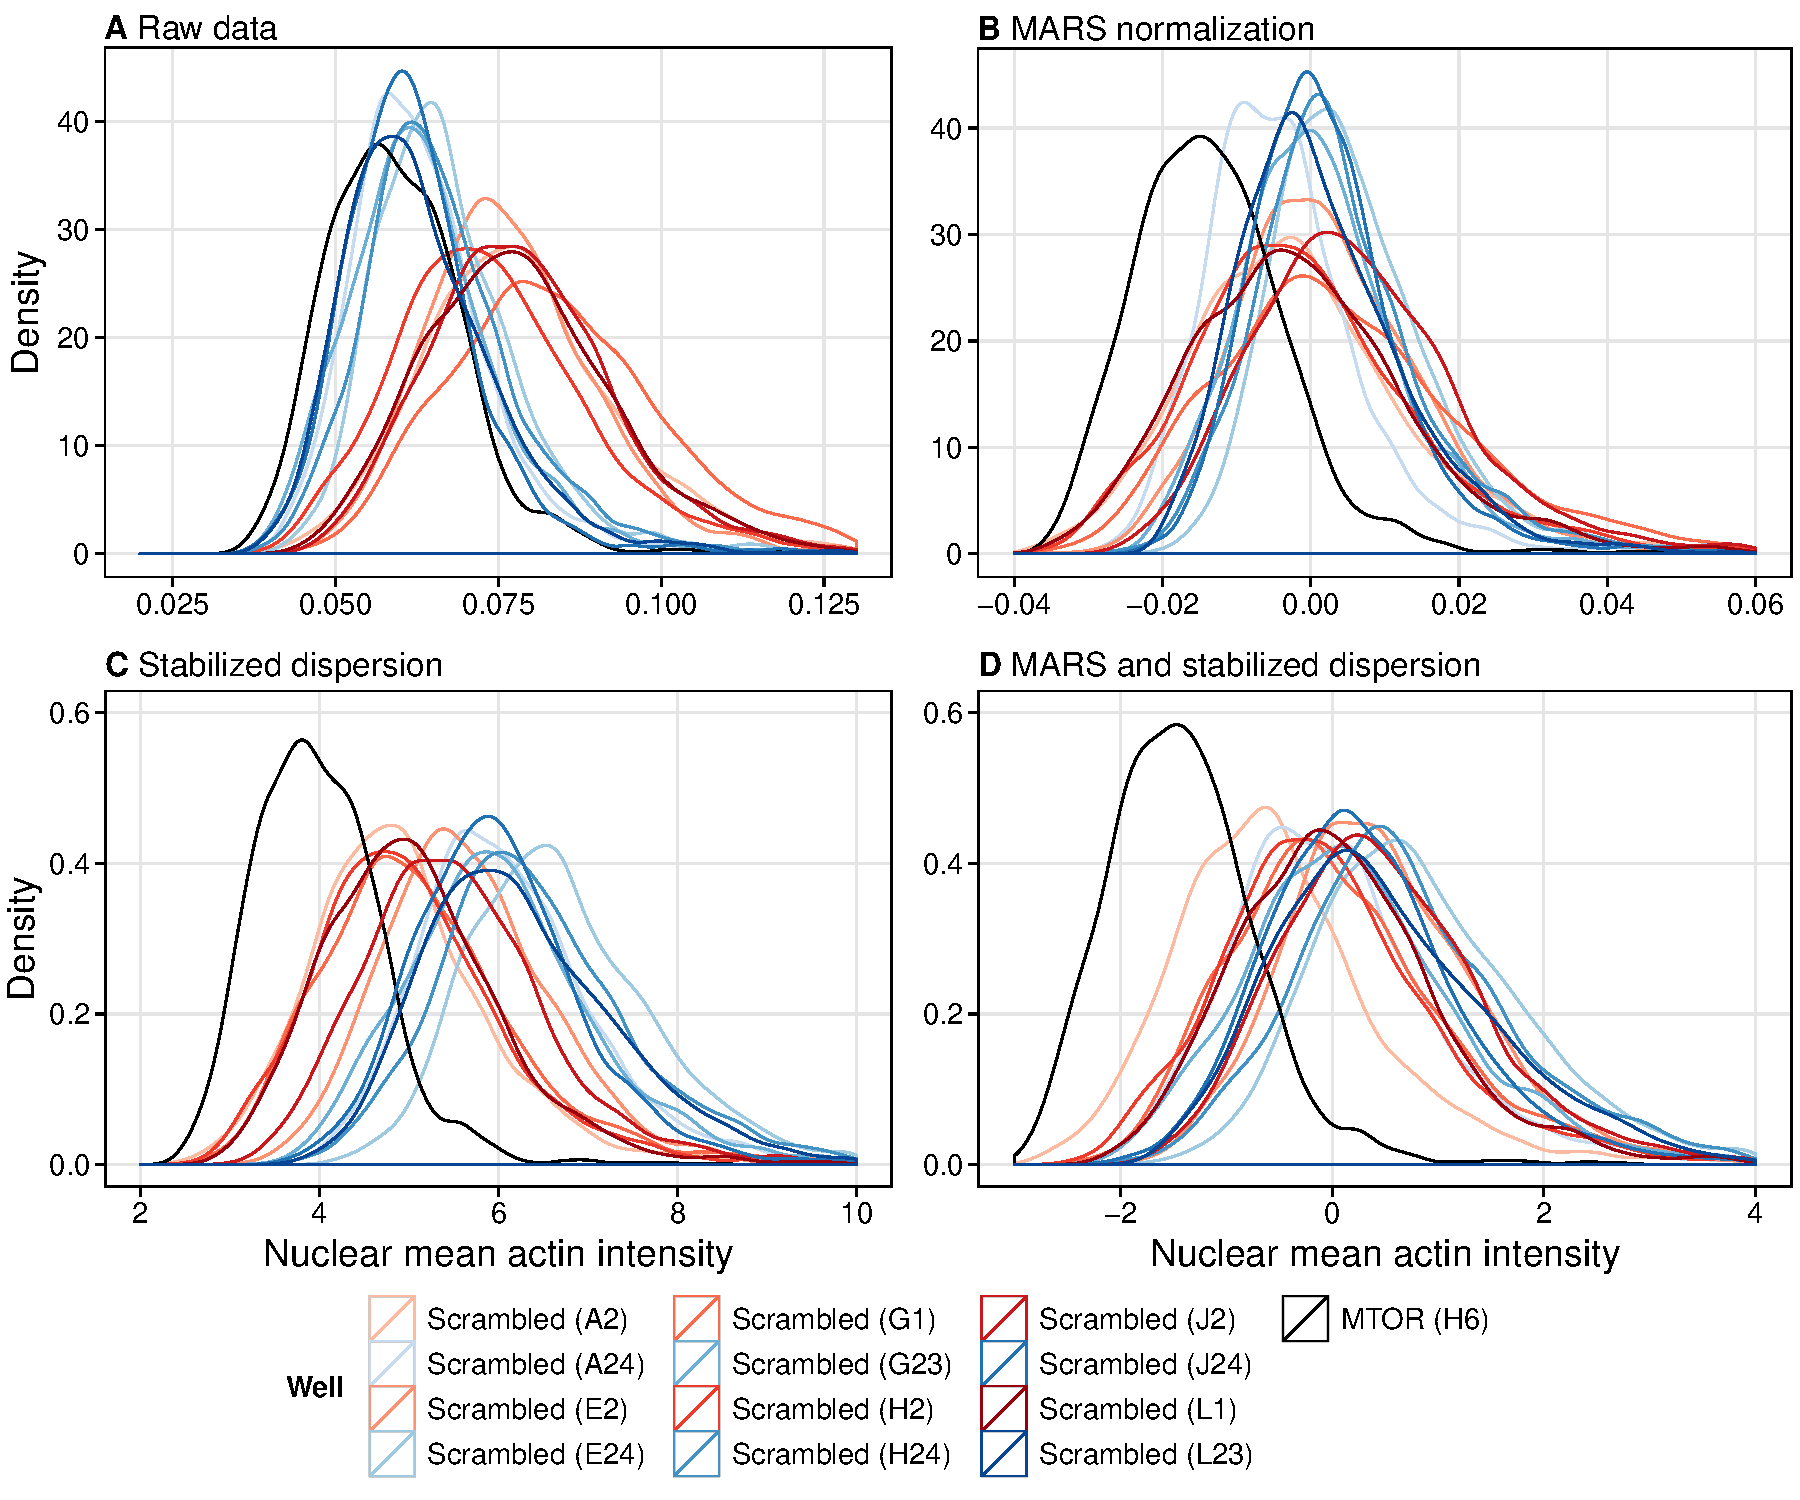
\includegraphics[width=\maxwidth]{figures/R/normalization-data-actin-normalization-1} 

}

\caption[Effects of normalization schemes visualized through density plots.]{In order to provide intuitive access to how normalization affects the data, four density plots are reproduced, using mean nuclear actin intensity of plate J110-2D. The top left plot represents the raw data and both a clear separation of two groups of scrambled wells (corresponding to early and late column wells) can be recognized, as well as the issue that differences between MTOR wells and scrambled wells appear no larger than differences among scrambled wells (A). Moving to the right partially recovers issues, as scrambled distributions now all roughly share the same center (B), while moving downwards improves the problem of varying dispersion with respect to scrambled grouping (C). Finally, bottom right represents a combination of both schemes, yielding the best result in that scrambled wells become more similar while differences to MTOR are retained (D).}\label{fig:data-actin-normalization}
\end{figure}


\end{knitrout}


Figure \ref{fig:data-actin-normalization} is reproduced for providing some intuition on effects that may be addressed by the proposed normalization schemes. Panel (A) represents raw nuclear mean actin intensity densities of all 12 scrambled wells and the single \ACRshort{mtor} well on a plate of the \textit{Brucella}, Dharmacon unpooled screen. Color coding of scrambled wells is based on the two groups that can easily be distinguished, which most probably are responsible for the alternating pattern of table \ref{tab:glm-1}. Wells that have a low column index are colored in shades of red, while late column wells are blue and colors grow darker with increasing row index. The density corresponding to \ACRshort{mtor} is shown in black.

With \cgls{mars} normalization, mainly due to B-scoring terms, the distance between the group centers are is drastically reduced without loosing information with respect to \ACRshort{mtor} (panel B of figure \ref{fig:data-actin-normalization}). Likewise for variance scaling (Z-scoring without centering), the previously distinct amount of dispersion within the two scrambled groups is equalized without affecting \ACRshort{mtor} (panel C). In order to make this step more robust, data is not divided by standard deviation, but by \cgls{mad} and while being carried out on well level, not only the individual wells are used for calculating \cgls{mad}, but the two vertical and horizontal neighbors are included as well (for plate borders, two neighboring wells on the same side of the target well are selected).

Finally, the two approaches can be coupled by first stabilizing dispersion, followed by \cgls{mars} normalization (panel D). For this particular feature, the hybrid approach yields the best results in the sense that discrepancies between scrambled wells are reduced without loosing information on \ACRshort{mtor}. Building on these results, one could assume that the combined normalization strategy should considerably improve \cgls{glm} modeling. However, while \cgls{mars} succeeds at recovering the data from column dependence, variance scaling does not help. Similarly for the two predictor sets in \cgls{mars}, the more complicated one does not yield better data quality. Therefore, the more parsimonious normalization procedure constituting only of \cgls{mars} targeted at technical issues was used to generate table \ref{tab:glm-2}.

\renewcommand{\arraystretch}{1.5}
\setlength{\tabcolsep}{0.25em}
\begin{table}
  \centering
  \caption[Reiteration of table \ref{tab:glm-1}, using normalized features for \cgls{glm} fitting.]{For illustrating the effect of \cgls{mars} normalization, using the smaller set of predictors targeted at technical issues only, this table is a reiteration of table \ref{tab:glm-1}, using normalized data instead. All other parameters (i.e. \cgls{pca}, 90\% of variance, etc.) remain. The following models suffer from separated data: \ACRshort{mtor} (A24, E2, E24, G1, G23, H2 and J2), \ACRshort{pik3r3} (H2), \ACRshort{ripk4} (A2, E24, G1, G23, H2, J2 and L1), Scrambled (G23 and H2) and \ACRshort{tgfbr1} (E2, E24 and H24).}
  \label{tab:glm-2}
  \footnotesize
  \vspace{5px}
  \begin{tabular}{llcccccccccccc}

 &  & A2 & A24 & E2 & E24 & G1 & G23 & H2 & H24 & J2 & J24 & L1 & \multicolumn{1}{c}{L23} \\ 
\hline
\nopagebreak MTOR & \nopagebreak AIC  & \multicolumn{1}{r}{2016} & \multicolumn{1}{r}{2187} & \multicolumn{1}{r}{1655} & \multicolumn{1}{r}{1458} & \multicolumn{1}{r}{1757} & \multicolumn{1}{r}{1448} & \multicolumn{1}{r}{1517} & \multicolumn{1}{r}{1268} & \multicolumn{1}{r}{1288} & \multicolumn{1}{r}{1736} & \multicolumn{1}{r}{2128} & \multicolumn{1}{r}{1860} \\
 & \nopagebreak \textDelta\textsubscript{deviance}  & \multicolumn{1}{r}{2821} & \multicolumn{1}{r}{2798} & \multicolumn{1}{r}{3151} & \multicolumn{1}{r}{3931} & \multicolumn{1}{r}{3203} & \multicolumn{1}{r}{3522} & \multicolumn{1}{r}{2846} & \multicolumn{1}{r}{3625} & \multicolumn{1}{r}{3632} & \multicolumn{1}{r}{3037} & \multicolumn{1}{r}{2723} & \multicolumn{1}{r}{3298} \\
 & \nopagebreak \textDelta\textsubscript{df}  & \multicolumn{1}{r}{47} & \multicolumn{1}{r}{48} & \multicolumn{1}{r}{48} & \multicolumn{1}{r}{47} & \multicolumn{1}{r}{47} & \multicolumn{1}{r}{47} & \multicolumn{1}{r}{48} & \multicolumn{1}{r}{47} & \multicolumn{1}{r}{48} & \multicolumn{1}{r}{47} & \multicolumn{1}{r}{48} & \multicolumn{1}{r}{48} \\
 & \rule{0pt}{1.7\normalbaselineskip}Acc  & \multicolumn{1}{r}{0.87} & \multicolumn{1}{r}{0.87} & \multicolumn{1}{r}{0.9} & \multicolumn{1}{r}{0.92} & \multicolumn{1}{r}{0.91} & \multicolumn{1}{r}{0.92} & \multicolumn{1}{r}{0.91} & \multicolumn{1}{r}{0.93} & \multicolumn{1}{r}{0.93} & \multicolumn{1}{r}{0.91} & \multicolumn{1}{r}{0.88} & \multicolumn{1}{r}{0.91} \\
 & \nopagebreak Mcc  & \multicolumn{1}{r}{0.75} & \multicolumn{1}{r}{0.74} & \multicolumn{1}{r}{0.79} & \multicolumn{1}{r}{0.83} & \multicolumn{1}{r}{0.82} & \multicolumn{1}{r}{0.84} & \multicolumn{1}{r}{0.81} & \multicolumn{1}{r}{0.85} & \multicolumn{1}{r}{0.86} & \multicolumn{1}{r}{0.82} & \multicolumn{1}{r}{0.77} & \multicolumn{1}{r}{0.82} \\
\rule{0pt}{1.7\normalbaselineskip}PIK3R3 & \nopagebreak AIC  & \multicolumn{1}{r}{4548} & \multicolumn{1}{r}{4095} & \multicolumn{1}{r}{4400} & \multicolumn{1}{r}{5149} & \multicolumn{1}{r}{4814} & \multicolumn{1}{r}{4833} & \multicolumn{1}{r}{3764} & \multicolumn{1}{r}{4143} & \multicolumn{1}{r}{4516} & \multicolumn{1}{r}{4371} & \multicolumn{1}{r}{4670} & \multicolumn{1}{r}{4839} \\
 & \nopagebreak \textDelta\textsubscript{deviance}  & \multicolumn{1}{r}{808} & \multicolumn{1}{r}{1430} & \multicolumn{1}{r}{920} & \multicolumn{1}{r}{849} & \multicolumn{1}{r}{686} & \multicolumn{1}{r}{680} & \multicolumn{1}{r}{1043} & \multicolumn{1}{r}{1278} & \multicolumn{1}{r}{937} & \multicolumn{1}{r}{912} & \multicolumn{1}{r}{701} & \multicolumn{1}{r}{889} \\
 & \nopagebreak \textDelta\textsubscript{df}  & \multicolumn{1}{r}{49} & \multicolumn{1}{r}{49} & \multicolumn{1}{r}{50} & \multicolumn{1}{r}{49} & \multicolumn{1}{r}{50} & \multicolumn{1}{r}{50} & \multicolumn{1}{r}{50} & \multicolumn{1}{r}{49} & \multicolumn{1}{r}{51} & \multicolumn{1}{r}{50} & \multicolumn{1}{r}{50} & \multicolumn{1}{r}{50} \\
 & \rule{0pt}{1.7\normalbaselineskip}Acc  & \multicolumn{1}{r}{0.72} & \multicolumn{1}{r}{0.77} & \multicolumn{1}{r}{0.67} & \multicolumn{1}{r}{0.67} & \multicolumn{1}{r}{0.68} & \multicolumn{1}{r}{0.68} & \multicolumn{1}{r}{0.76} & \multicolumn{1}{r}{0.76} & \multicolumn{1}{r}{0.69} & \multicolumn{1}{r}{0.72} & \multicolumn{1}{r}{0.67} & \multicolumn{1}{r}{0.68} \\
 & \nopagebreak Mcc  & \multicolumn{1}{r}{0.45} & \multicolumn{1}{r}{0.54} & \multicolumn{1}{r}{0.35} & \multicolumn{1}{r}{0.33} & \multicolumn{1}{r}{0.35} & \multicolumn{1}{r}{0.35} & \multicolumn{1}{r}{0.5} & \multicolumn{1}{r}{0.52} & \multicolumn{1}{r}{0.38} & \multicolumn{1}{r}{0.44} & \multicolumn{1}{r}{0.33} & \multicolumn{1}{r}{0.36} \\
\rule{0pt}{1.7\normalbaselineskip}RIPK4 & \nopagebreak AIC  & \multicolumn{1}{r}{4929} & \multicolumn{1}{r}{4862} & \multicolumn{1}{r}{5025} & \multicolumn{1}{r}{5995} & \multicolumn{1}{r}{5217} & \multicolumn{1}{r}{5303} & \multicolumn{1}{r}{4050} & \multicolumn{1}{r}{4677} & \multicolumn{1}{r}{5037} & \multicolumn{1}{r}{5221} & \multicolumn{1}{r}{5156} & \multicolumn{1}{r}{5574} \\
 & \nopagebreak \textDelta\textsubscript{deviance}  & \multicolumn{1}{r}{889} & \multicolumn{1}{r}{1146} & \multicolumn{1}{r}{751} & \multicolumn{1}{r}{550} & \multicolumn{1}{r}{764} & \multicolumn{1}{r}{692} & \multicolumn{1}{r}{1149} & \multicolumn{1}{r}{1214} & \multicolumn{1}{r}{891} & \multicolumn{1}{r}{514} & \multicolumn{1}{r}{679} & \multicolumn{1}{r}{665} \\
 & \nopagebreak \textDelta\textsubscript{df}  & \multicolumn{1}{r}{49} & \multicolumn{1}{r}{49} & \multicolumn{1}{r}{50} & \multicolumn{1}{r}{49} & \multicolumn{1}{r}{50} & \multicolumn{1}{r}{50} & \multicolumn{1}{r}{50} & \multicolumn{1}{r}{49} & \multicolumn{1}{r}{51} & \multicolumn{1}{r}{50} & \multicolumn{1}{r}{50} & \multicolumn{1}{r}{50} \\
 & \rule{0pt}{1.7\normalbaselineskip}Acc  & \multicolumn{1}{r}{0.69} & \multicolumn{1}{r}{0.72} & \multicolumn{1}{r}{0.67} & \multicolumn{1}{r}{0.64} & \multicolumn{1}{r}{0.69} & \multicolumn{1}{r}{0.64} & \multicolumn{1}{r}{0.76} & \multicolumn{1}{r}{0.75} & \multicolumn{1}{r}{0.71} & \multicolumn{1}{r}{0.63} & \multicolumn{1}{r}{0.68} & \multicolumn{1}{r}{0.67} \\
 & \nopagebreak Mcc  & \multicolumn{1}{r}{0.36} & \multicolumn{1}{r}{0.44} & \multicolumn{1}{r}{0.32} & \multicolumn{1}{r}{0.29} & \multicolumn{1}{r}{0.36} & \multicolumn{1}{r}{0.28} & \multicolumn{1}{r}{0.49} & \multicolumn{1}{r}{0.5} & \multicolumn{1}{r}{0.41} & \multicolumn{1}{r}{0.24} & \multicolumn{1}{r}{0.34} & \multicolumn{1}{r}{0.34} \\
\rule{0pt}{1.7\normalbaselineskip}Scrambled & \nopagebreak AIC  & \multicolumn{1}{r}{4495} & \multicolumn{1}{r}{4296} & \multicolumn{1}{r}{4699} & \multicolumn{1}{r}{5306} & \multicolumn{1}{c}{--} & \multicolumn{1}{r}{4951} & \multicolumn{1}{r}{4003} & \multicolumn{1}{r}{4921} & \multicolumn{1}{r}{5024} & \multicolumn{1}{r}{4462} & \multicolumn{1}{r}{4725} & \multicolumn{1}{r}{4740} \\
 & \nopagebreak \textDelta\textsubscript{deviance}  & \multicolumn{1}{r}{848} & \multicolumn{1}{r}{1217} & \multicolumn{1}{r}{607} & \multicolumn{1}{r}{679} & \multicolumn{1}{c}{--} & \multicolumn{1}{r}{549} & \multicolumn{1}{r}{795} & \multicolumn{1}{r}{491} & \multicolumn{1}{r}{416} & \multicolumn{1}{r}{809} & \multicolumn{1}{r}{634} & \multicolumn{1}{r}{976} \\
 & \nopagebreak \textDelta\textsubscript{df}  & \multicolumn{1}{r}{48} & \multicolumn{1}{r}{49} & \multicolumn{1}{r}{49} & \multicolumn{1}{r}{49} & \multicolumn{1}{c}{--} & \multicolumn{1}{r}{49} & \multicolumn{1}{r}{50} & \multicolumn{1}{r}{50} & \multicolumn{1}{r}{50} & \multicolumn{1}{r}{49} & \multicolumn{1}{r}{49} & \multicolumn{1}{r}{50} \\
 & \rule{0pt}{1.7\normalbaselineskip}Acc  & \multicolumn{1}{r}{0.69} & \multicolumn{1}{r}{0.73} & \multicolumn{1}{r}{0.65} & \multicolumn{1}{r}{0.64} & \multicolumn{1}{c}{--} & \multicolumn{1}{r}{0.66} & \multicolumn{1}{r}{0.67} & \multicolumn{1}{r}{0.66} & \multicolumn{1}{r}{0.58} & \multicolumn{1}{r}{0.66} & \multicolumn{1}{r}{0.62} & \multicolumn{1}{r}{0.72} \\
 & \nopagebreak Mcc  & \multicolumn{1}{r}{0.38} & \multicolumn{1}{r}{0.45} & \multicolumn{1}{r}{0.3} & \multicolumn{1}{r}{0.28} & \multicolumn{1}{c}{--} & \multicolumn{1}{r}{0.31} & \multicolumn{1}{r}{0.33} & \multicolumn{1}{r}{0.31} & \multicolumn{1}{r}{0.17} & \multicolumn{1}{r}{0.32} & \multicolumn{1}{r}{0.25} & \multicolumn{1}{r}{0.44} \\
\rule{0pt}{1.7\normalbaselineskip}TGFBR1 & \nopagebreak AIC  & \multicolumn{1}{r}{4414} & \multicolumn{1}{r}{4920} & \multicolumn{1}{r}{4105} & \multicolumn{1}{r}{4502} & \multicolumn{1}{r}{4429} & \multicolumn{1}{r}{4268} & \multicolumn{1}{r}{3250} & \multicolumn{1}{r}{3513} & \multicolumn{1}{r}{3817} & \multicolumn{1}{r}{4284} & \multicolumn{1}{r}{4709} & \multicolumn{1}{r}{4801} \\
 & \nopagebreak \textDelta\textsubscript{deviance}  & \multicolumn{1}{r}{1504} & \multicolumn{1}{r}{1194} & \multicolumn{1}{r}{1770} & \multicolumn{1}{r}{2162} & \multicolumn{1}{r}{1655} & \multicolumn{1}{r}{1832} & \multicolumn{1}{r}{2035} & \multicolumn{1}{r}{2481} & \multicolumn{1}{r}{2212} & \multicolumn{1}{r}{1549} & \multicolumn{1}{r}{1227} & \multicolumn{1}{r}{1549} \\
 & \nopagebreak \textDelta\textsubscript{df}  & \multicolumn{1}{r}{48} & \multicolumn{1}{r}{48} & \multicolumn{1}{r}{49} & \multicolumn{1}{r}{48} & \multicolumn{1}{r}{48} & \multicolumn{1}{r}{49} & \multicolumn{1}{r}{49} & \multicolumn{1}{r}{48} & \multicolumn{1}{r}{49} & \multicolumn{1}{r}{49} & \multicolumn{1}{r}{49} & \multicolumn{1}{r}{49} \\
 & \rule{0pt}{1.7\normalbaselineskip}Acc  & \multicolumn{1}{r}{0.76} & \multicolumn{1}{r}{0.71} & \multicolumn{1}{r}{0.78} & \multicolumn{1}{r}{0.77} & \multicolumn{1}{r}{0.76} & \multicolumn{1}{r}{0.76} & \multicolumn{1}{r}{0.82} & \multicolumn{1}{r}{0.83} & \multicolumn{1}{r}{0.82} & \multicolumn{1}{r}{0.76} & \multicolumn{1}{r}{0.73} & \multicolumn{1}{r}{0.74} \\
 & \nopagebreak Mcc  & \multicolumn{1}{r}{0.52} & \multicolumn{1}{r}{0.41} & \multicolumn{1}{r}{0.54} & \multicolumn{1}{r}{0.53} & \multicolumn{1}{r}{0.51} & \multicolumn{1}{r}{0.51} & \multicolumn{1}{r}{0.62} & \multicolumn{1}{r}{0.65} & \multicolumn{1}{r}{0.63} & \multicolumn{1}{r}{0.51} & \multicolumn{1}{r}{0.44} & \multicolumn{1}{r}{0.47} \\
\hline 
\end{tabular}


\end{table}

When comparing table \ref{tab:glm-2} to \ref{tab:glm-1}, the most striking difference is the disappearance of the striped pattern due to row dependence. This causes the previously very high prediction accuracies in scrambled wells to drop from \tilde 90\% to slightly more reasonable but still high \tilde 70\%. Furthermore, a clear difference between \ACRshort{mtor} and scrambled rows is discernible. \ACRshort{mtor} is consistently characterized by lower \cgls{aic} (about half), much larger $\Delta\textsubscript{deviance}$ (2--6 fold difference) and better prediction scores, altogether indicating better modeling of the differences between \ACRshort{mtor} and scrambled wells than of diversity within scrambled wells. \ACRshort{tgfbr1} results differ from scrambled as well (the same observation holds for table \ref{tab:glm-1}). Accuracies (and therefore \cglspl{mcc}) are generally lower for the control wells, while $\Delta\textsubscript{deviance}$ is 2--3 fold increased in \ACRshort{tgfbr1} wells. These observations are, however, put somewhat into perspective by the other 2 genes that do not exhibit behavior that is easily distinguishable from scrambled.
% map pc back to feats
% how about ridge, w/o pca?

\section{Outlook and Conclusion}
Unfortunately, the goal that was originally set out to achieve, to find a set of influential features that discriminate single cell data of infected cells between an \cgls{sirna} experiment targeting a hit gene and a scrambled control experiment, could so far not be accomplished. Such results may provide valuable insight into biological mechanisms as to how the down-regulated gene affects infection patterns, in turn, possibly yielding better understanding of pathogen infectivity in human cells. However, issues surrounding robust data normalization remain, despite much effort and prevent sensible inference from fitted models to be drawn. With current conditioning schemes, discrepancies between control wells persist to such an extent that biologically equivalent data can be separated witch 60--70\% accuracy (cf table \ref{tab:glm-2}), which is a clear indication of technical effects still being present to an unacceptable degree. Furthermore, the extent of inconsistencies among scrambled control wells is on the same order of magnitude as differences between wells containing \cgls{sirna} sequences against hit genes (with the exception of \ACRshort{mtor}), thereby making any possible list of influential features derived from current data highly questionable.

Issues of reproducibility have been plaguing \cgls{sirna} based \cgls{hts} ever since its conception and have recently gained attention with researchers calling for standardization of screening practice and more robust hit scoring. An example of the issue is provided by four \cgls{rnai} screens investigating \cgls{hiv} infection, performed in 2008 and 2009, three of which employ pooled \cgls{sirna} duplexes while the fourth uses pooled \cgls{shrna} reagents. On average, each of the screens reported 300 hit genes and interestingly, there is zero overlap among all four and only three genes are shared throughout the three \cgls{sirna} screens \citep{Bhinder2014}.

A large-scale study provided by \citet{Bhinder2013} corroborates concerns over reproducibility and quality of obtained hits. Out of a reviewed list of 300 published screening experiments, 30 lethality-based screens, performed by different research groups, were selected for comparative investigation. Aggregation of hits implicates a third of the overall genome, suggesting that an unlikely 30\% of all genes are essential to cellular survival. When investigating commonalities, not a single gene is reported throughout all screens. Constraining analysis to the 16 \cgls{sirna} screens (the other 14 use \cgls{shrna}), leaves two genome-wide and 14 focused studies and for both groups, 90\% of reported hits are specific to a single screen (orphan hits), while 4 genes are shared among the two genome wide and none are common to all focused experiments.

Such observations are mainly concerned with comparing the results of distinct investigations performed by separate research groups, possibly using individual procedures and a large source of variation must be attributed to the current lack of standard practice. Nevertheless, for utilizing \cgls{sirna} based \cgls{hts} at its full potential, issues of reproducibility must be resolved. To that end, much effort by InfectX has been dedicated to the development of a robust screening platform, providing as many replicates as possible and making data available publicly (a serious reproducibility issue is the nonavailability of raw data as it prevents others from examining and potentially improving data processing). Nevertheless, many technical artifacts, sources of variation intrinsic to \cgls{sirna} based experimentation, as well as the noisy nature of biological systems have to be handled.

While a fair amount of scrutiny towards data quality at well level, has led to some normalization procedures being developed for corresponding datasets, less work so far has been dedicated to the single cell level. As demonstrated, a combination of Z-scoring, B-scoring and a \cgls{mars} model as proposed by \citet{Knapp2011} is not sufficient for making single cell data of distinct wells directly comparable. Whether there are further technical effects that are not removed by this set of methods or biological issues that have not been considered are to blame is an open question. Further, it is unclear if correcting for population context is beneficial to the type of investigation at the heart of this project, as it might be overzealous in that cellular feature information that originates from \cgls{sirna} perturbations and manifests within population context is possibly removed.

\begin{figure}
  \centering
  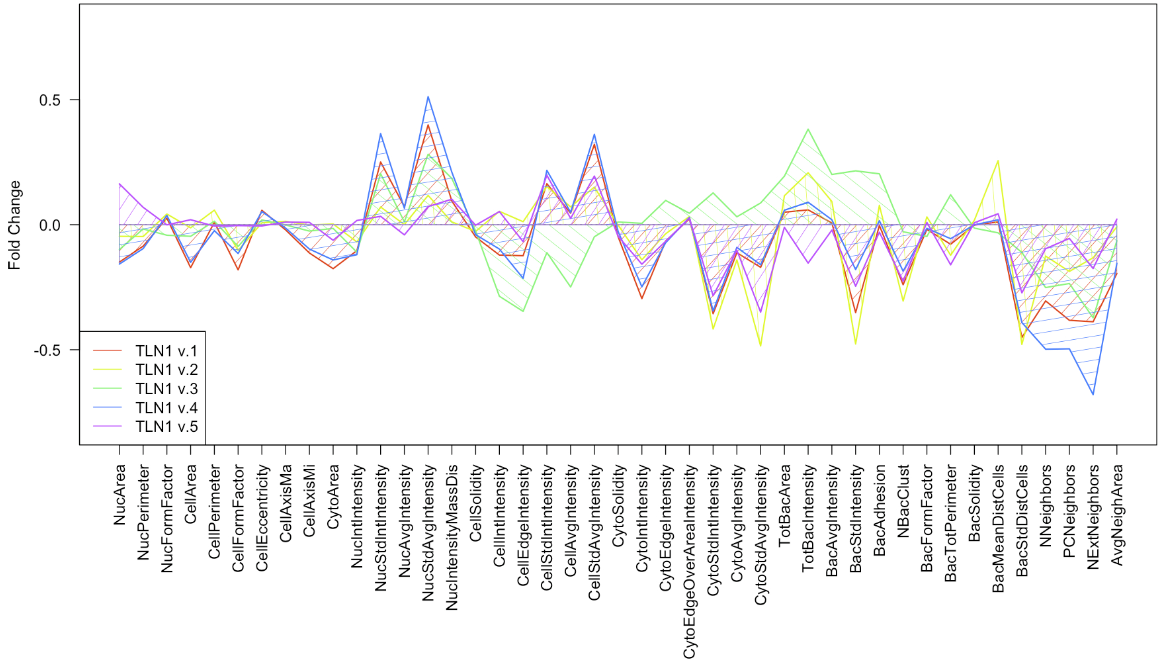
\includegraphics[width=0.95\textwidth]{sirna-variablilty}
  \caption[Feature space variability of different \cgls{sirna} sequences sharing the same target gene.]{A total of 5 distinct \cgls{sirna} sequences with the shared target \acrfull{tln1}, required for invasome formation in \textit{Bartonella} infection, yield considerable variability in feature space. While there are some commonalities, due to on-target effects, off targeting may cause individual behavior patterns. Figure take from \citet{Geier2010}.}
  \label{fig:sirna-variablilty}
\end{figure}

Instead of targeting population context related information, sources of variation such as \cglspl{ote} might provide more attractive objectives. Off-targeting has been established as an important confounding factor in \cgls{sirna} screening and it is entirely possible that some of the variability among scrambled control experiments is attributable to unintentional gene silencing. While scrambled seed sequences are specifically engineered not to match any known genes, especially \cglspl{3-utr}, the limited combinatorial space makes some degree of interaction likely. Furthermore, unspecific response may occur and add to the obfuscation of the actual signal. It might be possible to adapt recent developments in deconvolution of off-target confounded \cgls{rnai} screens, such as provided by \citet{Schmich2015} to the single cell level.

When only focusing on infected cells, the importance of correcting for \cglspl{ote} increases as wells of different sequences with the same target have to be aggregated in cases where the number of infected cells per single well is low (as is the case in \textit{Brucella} screens). The same holds for pooled \cgls{sirna} screens, as several nonidentical sequences with a common target are included in the same experiment. Distinguishing the signal of target knockdown from random perturbations constitutes a valuable improvement in such situations.

In addition to accounting for \cglspl{ote}, the present normalization scheme could be adapted to treat features individually, instead of repeatedly being applied in the same manner. There is great diversity among the multitude of features that are extracted from imagery which warrants further study. Perhaps individual data transformations need be applied and it may be necessary, albeit labor intensive to customize normalization at feature level. This was conceded but due to limited time availability so far could not be explored further.

If sufficient normalization proves elusive, changing the analysis setup has to be contemplated. Instead of determining influential features by comparing wells, modeling infected versus uninfected cells within a well might yield the desired insights. This alleviates the requirement of directly comparable wells while still determining well specific parameters. The features used for infection scoring are fixed pathogen wide and finding gene specific sets constitutes information that is qualitatively similar to that of the original investigation.

Finally, the number of available features is larger than the number of features considered during analysis and modeling. So far, only cellular features are included that are scalar valued per cell and provide a data point for each cell. Therefore pathogen objects and neighbor features are left out. This additional information could be included by developing appropriate augmentation functions such as location augmentation as implemented by singleCellFeatures. In that particular case, object coordinates which by themselves do not convey any directly interpretable information are transformed to more useful features, including local object density, distance from center, location within colonies, etc. Similarly, neighbor identity, again by itself not very useful, could be exploited to define object clusters and determine cluster area, cluster size in terms of members, number of infected members, and many other derived features. Adjacency matrices are assembled by singleCellFeatures and await being put to use.

While the desired list of influential features for \cgls{sirna} perturbed infection so far could not be compiled, a flexible and capable platform for manipulating the large amounts of data associated with single cell level, high throughput screening, was developed. More sophisticated normalization procedures have to be investigated and hopefully, building on lessons learnt from data analysis provided by this project, ways of extracting the initially targeted information from available datasets will be found in the future.


%%%%%%%%%%%%%%%%%%%%%%%%%%%%%%%%%%%%%%%%%%%%%%%%%%%%%%%%%%%%%%%%%%%%%%%%%%%%%%%
%%%  Appendices (if needed)                                                 %%%
%%%%%%%%%%%%%%%%%%%%%%%%%%%%%%%%%%%%%%%%%%%%%%%%%%%%%%%%%%%%%%%%%%%%%%%%%%%%%%%

\addtocontents{toc}{\vspace{.5\baselineskip}}
\appendix
\chapter{InfectX Protocols}

\section{Materials and Methods for Wet-Lab Procedures}
\label{sec:pathogen-protocols}
The following sections describe materials and methods employed in pathogen specific protocols. This information has been published in \citet{Ramo2014} and is only reproduced for the reader's convenience.

\paragraph{\textit{B. henselae}-specific protocol.}
\textit{Bartonella henselae} \acrshort{atcc}[49882\textsuperscript{T}] \textDelta\textit{bep}G containing plasmid pCD353 \citep{Dehio1998} for IPTG-inducible expression of \acrshort{gfp} were grown on \cgls{cba} plates supplemented with 5\% defibrinated sheep blood (Oxoid) and \SI{50}{\micro\gram\per\milli\litre} kanamycin. Bacteria were incubated at \SI{35}{\celsius} in 5\% \ce{CO2} for \SI{72}{\hour} before re-streaking them on fresh \cgls{cba} and further growth for \SI{48}{\hour}. Cells were washed once after \cgls{sirna}-transfection with M199 (Invitrogen)\slash 10\% \cgls{fbs} using a plate washer (ELx50-16, BioTek). Cells were infected with \textit{B. henselae} at an \cgls{moi} of 400 in \SI{50}{\micro\litre} of M199\slash 10\% \cgls{fbs} and \SI{0.5}{\milli\Molar} IPTG (Applichem) and were incubated at \SI{35}{\celsius} in 5\% \ce{CO2} for \SI{30}{\hour}. Fixation at \cgls{rtmp} was performed using a Multidrop 384 (Thermo Scientific) to wash cells with \SI{50}{\micro\litre} of \cgls{pbs}, fixed in \SI{20}{\micro\litre} of 3.7\% \cgls{pfa} for \SI{10}{\minute}, and washed once more with \SI{50}{\micro\litre} of \cgls{pbs}. Staining was performed on a Biomek liquid handling platform. Fixed cells were washed twice with \SI{25}{\micro\litre} of \cgls{pbs} and blocked in \cgls{pbs}\slash 0.2\% \cgls{bsa} for \SI{10}{\minute}. Extracellular bacteria were labeled with a rabbit serum 2037 against B. henselae \citep{Dehio1997} and a secondary antibody goat anti rabbit A647 (Jackson Immuno) in \cgls{pbs}\slash 0.2\% \cgls{bsa}. Antibodies were incubated for \SI{30}{\minute} each and both incubations were followed by two washings with \SI{25}{\micro\litre} of \cgls{pbs}. Cells were then permeabilized with \SI{20}{\micro\litre} of 0.1\% Triton X-100 (Sigma) for \SI{10}{\minute} and afterwards washed twice with \SI{25}{\micro\litre} of \cgls{pbs}, followed by the addition of \SI{20}{\micro\litre} of staining solution (\cgls{pbs} containing \SI{1.5}{\micro\gram\per\milli\litre} DY-547-Phalloidin, Dyomics and \SI{1}{\micro\gram\per\milli\litre} \cgls{dapi}, Roche). After \SI{30}{\minute} of incubation in the staining solution, cells were washed twice with \SI{25}{\micro\litre} \cgls{pbs}, followed by a final addition of \SI{50}{\micro\litre} of \cgls{pbs}.

\paragraph{\textit{B. abortus}-specific protocol.}
\textit{Brucella abortus} 2308 pJC43 (\textit{aphT::\acrshort{gfp}}) \citep{Celli2005} were grown in \cgls{tsb} medium containing \SI{50}{\micro\gram\per\milli\litre} kanamycin for \SI{20}{\hour} at \SI{37}{\celsius} and shaking (\SI{100}{\rpm}) to an OD of 0.8--1.1. \SI{50}{\micro\litre} of \acrshort{dmem}\slash 10\% containing bacteria was added per well to obtain a final \cgls{moi} of 10000 using a cell plate washer (ELx50-16, BioTek). Plates were then centrifuged at \SI{400}{\gravity} for \SI{20}{\minute} at \SI{4}{\celsius} to synchronize bacterial entry. After \SI{4}{\hour} incubation at \SI{37}{\celsius} and 5\% \ce{CO2}, extracellular bacteria were killed by exchanging the infection medium by \SI{50}{\micro\litre} medium supplemented with 10\% \cgls{fbs} and \SI{100}{\micro\gram\per\milli\litre} gentamicin (Sigma). After a total infection time of \SI{44}{\hour} cells were fixed with 3.7\% \cgls{pfa} for \SI{20}{\minute} at \cgls{rtmp} with the cell plate washer. Staining was performed using a Biomek liquid handling platform. Cells were washed twice with \cgls{pbs} and permeabilized with 0.1\% Triton X (Sigma) for \SI{10}{minute}. Then, cells were washed twice with \cgls{pbs}, followed by addition of \SI{20}{\micro\litre} of staining solution which includes \cgls{dapi} (\SI{1}{\micro\gram\per\milli\litre}, Roche) and DY-547-phalloidin (\SI{1.5}{\micro\gram\per\milli\litre}, Dyomics) in 0.5\% \cgls{bsa} in \cgls{pbs}. Cells were incubated with staining solution for \SI{30}{\minute} at \cgls{rtmp}, washed twice with \cgls{pbs}, followed by final addition of \SI{50}{\micro\litre} \cgls{pbs}.

\paragraph{\textit{L. monocytogenes}-specific protocol.}
After washing an overnight culture of \textit{Listeria monocytogenes} EGDe.PrfA*\acrshort{gfp} three times with \cgls{pbs}, bacteria were diluted in \acrshort{dmem} supplemented with 1\% \cgls{fbs}. Cells were infected at a \cgls{moi} of 25 in \SI{30}{\micro\litre} infection medium per well. After centrifugation at \SI{1000}{\rpm} for \SI{5}{\minute} and incubation for \SI{1}{\hour} at \SI{37}{\celsius} in 5\% \ce{CO2} to allow the bacteria to enter, extracellular bacteria were killed by exchanging the infection medium by \SI{30}{\micro\litre} \acrshort{dmem} supplemented with 10\% \cgls{fbs} and \SI{40}{\micro\gram\per\milli\litre} gentamicin (Gibco). Both medium exchange steps were carried out with a plate washer (ELx50-16, BioTek). After additional \SI{4}{\hour} at \SI{37}{\celsius} in a 5\% \ce{CO2} atmosphere, cells were fixed for \SI{15}{\minute} at \cgls{rtmp} by adding \SI{30}{\micro\litre} of 8\% \cgls{pfa} in \cgls{pbs} to each well using a multidrop 384 device (Thermo Electron Corporation). \cgls{pfa} was removed by four washes with \SI{500}{\micro\litre} \cgls{pbs} per well using the Power Washer 384 (Tecan). Fixed cells were stained for nuclei, actin and bacterially secreted \acrshort{inl}[C]. First, cells were incubated for \SI{30}{\minute} with \SI{10}{\micro\litre} per well of primary staining solution (0.2\% saponin, \cgls{pbs}) containing rabbit derived anti-\acrshort{inl}[C] serum (1:250). After four washes with \SI{40}{\micro\litre} \cgls{pbs} per well cells were stained with \SI{10}{\micro\litre} per well of the secondary staining solution (0.2\% saponin, \cgls{pbs}) containing Alexa Fluor-546 coupled anti-rabbit antibody (1:250, Invitrogen), \cgls{dapi} (\SI{0.7}{\micro\gram\per\milli\litre}, Roche), and DY-647-Phalloidin (\SI{2}{\micro\gram\per\milli\litre}, Dyomics). After four washes with \SI{40}{\micro\litre} \cgls{pbs} per well, the cells were kept in \SI{40}{\micro\litre} \cgls{pbs} per well. The staining procedure was carried out with a Tecan freedom evo robot.

\paragraph{\textit{S.} typhimurium-specific protocol.}
All liquid handing stages of infection, fixation, and immunofluorescence staining were performed on a liquid handling robot (BioTek; EL406). For infection the \textit{S.} typhimurium strain S.Tm\textsuperscript{SopE\_pM975} was used. This strain is a single effector strain, only expressing SopE out of the main four \acrshort{spi}[-1] encoded effectors (\acrshort{sip}[A], \acrshort{sop}[B], \acrshort{sop}[E2] and \acrshort{sop}[E]). Additionally this strain harbors a plasmid (pM975) that expresses \acrshort{gfp} under the control of a \acrshort{spi}[-2] (\acrshort{ssa}[G])-dependent promotor. The bacterial solution was prepared by cultivating a \SI{12}{\hour} culture in \SI{0.3}{\Molar} \cgls{lb} medium containing \SI{50}{\micro\gram\per\milli\litre} streptomycin and \SI{50}{\micro\gram\per\milli\litre} ampicillin. Afterwards a \SI{4}{\hour} subculture (1:20 diluted from the \SI{12}{\hour} culture) was cultivated in \SI{0.3}{\Molar} \cgls{lb} medium containing \SI{50}{\micro\gram\per\milli\litre} streptomycin, which reached an OD\textunderscript{\SI{600}{\nano\meter}}$\approx1.0$ after the respective \SI{4}{\hour} of incubation time. To perform the infection, \SI{16}{\micro\litre} of diluted \textit{S.} typhimurium (\cgls{moi} of 80) were added to the HeLa cells. After \SI{20}{\minute} of incubation at \SI{37}{\celsius} and 5\% \ce{CO2}, the \textit{S.} typhimurium-containing media was replaced by \SI{60}{\micro\litre} \acrshort{dmem}\slash 10\% \cgls{fbs} containing \SI{50}{\micro\gram\per\micro\litre} streptomycin and \SI{400}{\micro\gram\per\micro\litre} gentamicin to kill all remaining extracellular bacteria. After additional \SI{3}{\hour} \SI{40}{\minute} incubation at \SI{37}{\celsius} and 5\% \ce{CO2}, cells were fixed by adding \SI{35}{\micro\litre} 4\% \cgls{pfa}, 4\% sucrose in \cgls{pbs} for \SI{20}{\minute} at \cgls{rtmp}. The fixation solution was removed by adding \SI{60}{\micro\litre} \cgls{pbs} containing \SI{400}{\micro\gram\per\milli\litre} gentamicin. Cells were permeabilized for \SI{5}{\minute} with \SI{40}{\micro\litre} 0.1\% Triton X-100 (Sigma-Aldrich). Afterwards \SI{24}{\micro\litre} of staining solution containing \cgls{dapi} (1:1000, Sigma-Aldrich) and DY-547-phalloidin (\SI{1.2}{\micro\gram\per\milli\litre}, Dyomics) was added (prepared in blocking buffer consisting of 4\% \cgls{bsa} and 4\% Sucrose in \cgls{pbs}). After \SI{1}{\hour} of incubation at \cgls{rtmp}, cells were washed three times with \cgls{pbs} followed by the addition of \SI{60}{\micro\litre} \cgls{pbs} containing \SI{400}{\micro\gram\per\milli\litre} gentamicin.

\paragraph{\textit{S. flexneri}-specific protocol.}
\textit{Shigella flexneri} M90T \textDelta\textit{vir}G pCK100 (PuhpT::ds\-Red) were harvested in exponential growth phase and coated with 0.005\% poly-L-lysine (Sigma-Aldrich). Afterwards, bacteria were washed with \cgls{pbs} and resuspended in assay medium (\acrshort{dmem}, \SI{2}{\milli\Molar} L-Glutamine, \SI{10}{\milli\Molar} HEPES). \SI{20}{\micro\litre} of bacterial suspension was added to each well with a final \cgls{moi} of 15. Plates were then centrifuged for \SI{1}{\minute} at \SI{37}{\celsius} and incubated at \SI{37}{\celsius} and 5\% \ce{CO2}. After \SI{30}{\minute} of infection, \SI{75}{\micro\litre} were aspirated from each well and monensin (Sigma) and gentamicin (Gibco) were added to a final concentration of \SI{66.7}{\micro\Molar} and \SI{66.7}{\micro\gram\per\milli\litre}, respectively. After a total infection time of \SI{3.5}{\hour}, cells were fixed in 4\% \cgls{pfa} for \SI{10}{\minute}. Liquid handling was performed using the Multidrop 384 (Thermo Scientific) for dispension steps and a plate washer (ELx50-16, BioTek) for aspiration steps. For immunofluorescent staining, cells were washed with \cgls{pbs} using the Power Washer 384 (Tecan). Subsequently, cells were incubated with a mouse anti-human \cgls{il-8} antibody (1:300, BD Biosciences) in staining solution (0.2\% saponin in \cgls{pbs}) for \SI{2}{\hour} at \cgls{rtmp}. After washing the cells with \cgls{pbs}, Hoechst (\SI{5}{\micro\gram\per\milli\litre}, Invitrogen), DY-495-phalloidin (\SI{1.2}{\micro\gram\per\milli\litre}, Dyomics) and Alexa Fluor 647-coupled goat anti-mouse IgG (1:400, Invitrogen) were added and incubated for \SI{1}{\hour} at \cgls{rtmp}. The staining procedure was performed using the Biomek NXP Laboratory Automation Workstation (Beckman Coulter).

\paragraph{Adenovirus-specific protocol.}
All liquid handling stages of infection, fixation, and immunofluorescence staining were performed on the automated pipetting system Well Mate (Thermo Scientific Matrix) and washer Hydrospeed (Tecan). For infection screens recombinant Ad2\_\textDelta E3B-e\acrshort{gfp} (short Adenovirus) was utilized as described before \citep{Suomalainen2013,Yakimovich2012}. Adenovirus was added to cells at an \cgls{moi} of 0.1 in \SI{10}{\micro\litre} of an infection media\slash \cgls{fbs} (\acrshort{dmem} supplemented with L-glutamine, 10\% \cgls{fbs}, 1\% Pen\slash Strep, Invitrogen). Screening plates were incubated at \SI{37}{\celsius} for \SI{16}{\hour}, and cells were fixed by adding \SI{21}{\micro\litre} of 16\% \cgls{pfa} directly to the cells in culture media for \SI{45}{\minute} at \cgls{rtmp} or long-term storage at \SI{4}{\celsius}. Cells were washed 2 times with \cgls{pbs}\slash \SI{25}{\milli\Molar} \ce{NH4Cl}, permeabilized with \SI{25}{\micro\litre} 0.1\% Triton X-100 (Pharmaciebiothek). After 2 washes with \cgls{pbs} the samples were incubated at \cgls{rtmp} for \SI{1}{\hour} with \SI{25}{\micro\litre} staining solution (\cgls{pbs}) containing \cgls{dapi} (\SI{1}{\micro\gram\per\milli\litre}, Sigma-Aldrich) and DY-647-phalloidin (\SI{1}{\micro\gram\per\milli\litre}, Dyomics), washed 2 times with \cgls{pbs} and stored until imaging in \SI{50}{\micro\litre} \cgls{pbs}\slash \ce{NaN3}.

\paragraph{Rhinovirus-specific protocol.}
All liquid handling stages of infection, fixation, and immunofluorescence staining were performed on the automated pipetting system Well Mate (Thermo Scientific Matrix) and washer Hydrospeed (Tecan). For infection assays with human Rhinovirus serotype 1a (HRV1a) were carried out as described, except that the anti-VP2 antibody Mab 16\slash 7 was used for staining of the infected cells as described earlier \citep{Jurgeit2012,Jurgeit2010,Mosser2002}. Rhinovirus at an \cgls{moi} of 8 was added to cells in \SI{20}{\micro\litre} of an infection media\slash \cgls{bsa} (\acrshort{dmem} supplemented with GlutaMAX, \SI{30}{\milli\Molar} \ce{MgCl2} and 0.2\% \cgls{bsa}, Invitrogen). Screening plates were incubated for \SI{7}{\hour} at \SI{37}{\celsius}, and cells were fixed by adding \SI{33}{\micro\litre} of 16\% \cgls{pfa} directly to the culture medium. Fixation was either for \SI{30}{\minute} at \cgls{rtmp} or long term storage at \SI{4}{\celsius}. Cells were washed twice with \cgls{pbs}\slash \SI{25}{\milli\Molar} \ce{H2O}, permeabilized with \SI{50}{\micro\litre} 0.2\% Triton X-100 (Sigma- Aldrich) followed by 3 \cgls{pbs} washes and blocking with \cgls{pbs} containing 1\% \cgls{bsa} (Fraction V, Sigma-Aldrich). Fixed and permeabilized cells were incubated at \cgls{rtmp} for \SI{1}{\hour} with diluted mabR16-7 antibody (\SI{0.45}{\micro\gram\per\milli\litre}) in \cgls{pbs}\slash 1\% \cgls{bsa}. Cells were washed 3 times with \cgls{pbs} and incubated with \SI{25}{\micro\litre} secondary staining solution (\cgls{pbs}\slash 1\% \cgls{bsa}) containing Alexa Fluor 488 secondary antibody (\SI{1}{\micro\gram\per\milli\litre}, Invitrogen), \cgls{dapi} (\SI{1}{\micro\gram\per\milli\litre}, Sigma-Aldrich), and DY-647-phalloidin (\SI{0.2}{\micro\gram\per\milli\litre}, Dyomics). Cells were washed twice with \cgls{pbs} after \SI{2}{\hour} of incubation in secondary staining solution and stored in \SI{50}{\micro\litre} \cgls{pbs}\slash \ce{NaN3}.

\paragraph{Vacciniavirus-specific protocol.}
All liquid handing stages of infection, fixation, and immunofluorescence staining were performed on a liquid handling robot (BioTek, EL406). For infection assays a recombinant WR VACV, WR E E\acrshort{gfp}\slash L mCherry, was utilized. For infection, media was aspirated from the \cgls{rnai}-transfected cell plates and replaced with \SI{40}{\micro\litre} of virus solution per well (\cgls{moi} of 0.125). Screening plates were incubated for \SI{1}{\hour} at \SI{37}{\celsius} to allow for infection, after which virus-containing media was removed and replaced with \SI{40}{\micro\litre} \acrshort{dmem}\slash 10\% \cgls{fbs}. \SI{8}{\hour} after infection \SI{40}{\micro\litre} of \acrshort{dmem}\slash 10\% \cgls{fbs} containing \SI{20}{\micro\Molar} cytosine arabinoside (AraC) was added to all wells to prevent virus \cgls{dna} replication in secondary infected cells. \SI{24}{\hour} after infection cells were fixed by the addition of \SI{20}{\micro\litre} 18\% \cgls{pfa} for \SI{30}{\minute} followed by two \cgls{pbs} washes of \SI{80}{\micro\litre}. For immunofluorescence staining of E\acrshort{gfp}, cells were incubated for \SI{2}{\hour} in \SI{30}{\micro\litre} primary staining solution (0.5\% Triton X-100, 0.5\% \cgls{bsa}, \cgls{pbs}) per well, containing anti-\acrshort{gfp} antibody (1:1000). Cells were washed twice in \SI{80}{\micro\litre} \cgls{pbs}, followed by the addition of \SI{30}{\micro\litre} secondary staining solution (0.5\% \cgls{bsa}, \cgls{pbs}) containing Alexa Fluor 488 secondary antibody (1:1000), Hoechst (1:10000), and DY-647-phalloidin (1:1200, Dyomics). Cells were washed twice with \SI{80}{\micro\litre} \cgls{pbs} after \SI{1}{\hour} incubation in secondary staining solution followed by the addition of \SI{80}{\micro\litre} \ce{H2O}.

\section{Decision Trees for Infection Scoring}
\label{sec:app-dectree}
The decision trees for adenovirus and \textit{Bartonella} are shown in section~\ref{sec:infection-scoring} while the ones corresponding to the remaining pathogens (\textit{Brucella}, \textit{Listeria}, rhino\-virus, \textit{Salmonella} and vaccinia virus) follow\footnote{\textit{Shigella} infection scoring currently does not rely on \cgls{dtis}, therefore no decision tree is shown. Please refer to section~\ref{sec:infection-scoring} for details on detection of infected cells in \textit{Shigella} screens.}. Please refer to section~\ref{sec:infection-scoring} for more information of infection scoring, including descriptions of infection patterns upon which these decision trees are based. The corresponding tables show the different thresholds that currently are in use. Due to several experimental parameters affecting intensity measurements, such as age of microscope lamp, plate position in imaging queue or quality of staining, plate-wise adjustments are necessary in some instances. Several plates can be subjected to the same values, but over all datasets, some variation exists. Accompanying each of the following decision trees is a table holding the currently used sets of decision boundaries alongside a percentage value indicating the coverage of a given parameter set. For \textit{Brucella} and vaccinia, only the 12 most frequent sets are printed, while the lists for the remaining pathogens are exhaustive.

\renewcommand{\arraystretch}{1.5}
\setlength{\tabcolsep}{0.38em}
\begin{figure}[t!]
  \centering
  \begin{tikzpicture}
    \node [decision={$> \text{A}$}{$\le \text{A}$}] { 
      \texttt{Nuclei.Intensity\_MeanIntensity\_\\CorrPathogen}
    }
    [decision tree]
    child { node [infected] { infected } }
    child { node [decision={$> \text{B}$}{$\le \text{B}$}] { 
    \texttt{PeriNuclei.Intensity\_\\MeanIntensity\_CorrPathogen} } 
      child { node [infected] { infected } }
      child { node [decision={$> \text{C}$}{$\le \text{C}$}] { 
      \texttt{Cells.Intensity\_MeanIntensity\_\\CorrPathogen} }
        child { node [infected] { infected } }
        child { node [healthy] { not infected } }
      }
    };
  \end{tikzpicture}

  \vspace{5mm}
  \footnotesize
  % latex table generated in R 3.2.3 by xtable 1.7-4 package
% Sat Jan 16 10:48:22 2016
\begin{tabular}{ccccccccccccc}
   \hline
A & 0.050 & 0.050 & 0.060 & 0.075 & 0.045 & 0.050 & 0.040 & 0.055 & 0.050 & 0.040 & 0.050 & 0.040 \\ 
  B & 0.055 & 0.055 & 0.065 & 0.090 & 0.050 & 0.055 & 0.045 & 0.060 & 0.055 & 0.045 & 0.055 & 0.045 \\ 
  C & 0.075 & 0.070 & 0.085 & 0.105 & 0.070 & 0.070 & 0.075 & 0.080 & 0.075 & 0.065 & 0.070 & 0.065 \\ 
  Abundance & 31\% & 9\% & 9\% & 8\% & 7\% & 4\% & 3\% & 3\% & 3\% & 3\% & 3\% & 3\% \\ 
   \hline
\end{tabular}


  \vspace{5mm}
  \caption[Decision tree for \textit{Brucella} infection scoring.]{Decision tree for \textit{Brucella} infection scoring. While the first two decisions are modeled to capture what is considered a normal infection pattern, the last split imposes a high threshold for cells that have failed the first two steps to still be considered infected. The list of decision boundaries values is not exhaustive and the remaining 14\% of plates is handled by an additional 29 parameter sets.}
\end{figure}

\begin{figure}
  \centering
  \begin{tikzpicture}
    \node [decision={$> \text{A}$}{$\le \text{A}$}] { 
      \texttt{Nuclei.Intensity\_MeanIntensity\_\\CorrInlC}
    }
    [decision tree]
    child { node [infected] { infected } }
    child { node [decision={$> \text{B}$}{$\le \text{B}$}] { 
    \texttt{PeriNuclei.Intensity\_\\MeanIntensity\_CorrInlC} } 
      child { node [infected] { infected } }
      child { node [decision={$> \text{C}$}{$\le \text{C}$}] { 
      \texttt{Nuclei.Intensity\_UpperQuartile-\\Intensity\_CorrInlC} }
        child { node [infected] { infected } }
        child { node [healthy] { not infected } }
      }
    };
  \end{tikzpicture}

  \vspace{5mm}
  \footnotesize
  % latex table generated in R 3.2.3 by xtable 1.7-4 package
% Fri Jan 15 18:38:18 2016
\begin{tabular}{cccccccccc}
   \hline
A & 0.11 & 0.29 & 0.28 & 0.21 & 0.20 & 0.32 & 0.30 & 0.22 & 0.19 \\ 
  B & 0.15 & 0.36 & 0.35 & 0.28 & 0.27 & 0.39 & 0.37 & 0.29 & 0.26 \\ 
  C & 0.12 & 0.31 & 0.30 & 0.23 & 0.22 & 0.34 & 0.32 & 0.24 & 0.21 \\ 
  Abundance & 25\% & 12\% & 12\% & 12\% & 12\% & 6\% & 6\% & 6\% & 6\% \\ 
   \hline
\end{tabular}


  \vspace{5mm}
  \caption[Decision tree for \textit{Listeria} infection scoring.]{The decision tree for \textit{Listeria} infection scoring is based on a channel recording \acrshort{inl}[C] localization and intensity instead of targeting the bacteria themselves. Despite the values indicating coverage of each of the parameter sets not summing to unity, the list is exhaustive. The discrepancy is caused by rounding.}
\end{figure}

\begin{figure}
  \centering
  \begin{tikzpicture}
    \node [decision={$> \text{A}$}{$\le \text{A}$}] { 
      \texttt{Nuclei.Intensity\_MeanUpperTen-\\PercentIntensity\_CorrPathogen}
    }
    [decision tree]
    child { node [infected] { infected } }
    child { node [decision={$> \text{B}$}{$\le \text{B}$}] { 
    \texttt{PeriNuclei.Intensity\_MeanUpperTen-\\PercentIntensity\_CorrPathogen} } 
      child { node [infected] { infected } }
      child { node [decision={$> \text{C}$}{$\le \text{C}$}] { 
      \texttt{VoronoiCells.Intensity\_MeanUpper-\\TenPercentIntensity\_CorrPathogen} }
        child { node [infected] { infected } }
        child { node [healthy] { not infected } }
      }
    };
  \end{tikzpicture}

  \vspace{5mm}
  \footnotesize
  % latex table generated in R 3.2.3 by xtable 1.7-4 package
% Sat Jan 16 10:48:22 2016
\begin{tabular}{cccccc}
   \hline
A & 0.095 & 0.090 & 0.085 & 0.115 & 0.080 \\ 
  B & 0.100 & 0.095 & 0.090 & 0.125 & 0.085 \\ 
  C & 0.140 & 0.130 & 0.125 & 0.165 & 0.120 \\ 
  Abundance & 45\% & 35\% & 14\% & 5\% & 1\% \\ 
   \hline
\end{tabular}


  \vspace{5mm}
  \caption[Decision tree for rhinovirus infection scoring.]{Decision tree for rhinovirus infection scoring. Using the mean of the uppermost decile of pathogen channel intensity data yields the most stable results.}
\end{figure}

\begin{figure}
  \centering
  \begin{tikzpicture}
    \node [decision={$> \text{A}$}{$\le \text{A}$}] { 
      \texttt{Cells.Intensity\_SubCellBacteria-\\MeanIntensity\_CorrPathogen}
    }
    [decision tree]
    child { node [decision={$< \text{B}$}{$\ge \text{B}$}] { 
      \texttt{Cells.AreaShape\_SubCellBacteria-\\Area\_CorrPathogen} }
      child { node [infected] { infected } }
      child { node [healthy] { not infected } }
    }
    child { node [healthy] { not infected } };
  \end{tikzpicture}

  \vspace{5mm}
  \footnotesize
  % latex table generated in R 3.2.3 by xtable 1.7-4 package
% Fri Jan 15 18:38:18 2016
\begin{tabular}{ccccccccccccc}
   \hline
A & 0.095 & 0.100 & 0.068 & 0.070 & 0.082 & 0.085 & 0.090 & 0.067 & 0.105 & 0.080 & 0.065 & 0.069 \\ 
  B & 2 & 2 & 2 & 2 & 2 & 2 & 2 & 2 & 2 & 2 & 2 & 2 \\ 
  Abundance & 41\% & 11\% & 9\% & 7\% & 7\% & 6\% & 6\% & 6\% & 2\% & 2\% & 2\% & 2\% \\ 
   \hline
\end{tabular}


  \vspace{5mm}
  \caption[Decision tree for \textit{Salmonella} infection scoring.]{Decision tree for \textit{Salmonella} infection scoring. For a cell being considered infected, not only does the threshold for pathogen intensity throughout the cell need be exceeded but the bacteria also have to be sufficiently aggregated. The list of decision boundaries is exhaustive and the sum of coverage percentages overshooting unity is caused by rounding.}
  \label{fig:dectree-salmonella}
\end{figure}

\begin{figure}
  \centering
  \begin{tikzpicture}
    \node [decision={$> \text{A}$}{$\le \text{A}$}] { 
      \texttt{Nuclei.Intensity\_MeanIntensity\_\\Corr1Pathogen}
    }
    [decision tree]
    child { node [infected] { infected } }
    child { node [decision={$> \text{B}$}{$\le \text{B}$}] { 
    \texttt{PeriNuclei.Intensity\_\\MeanIntensity\_Corr1Pathogen} } 
      child { node [infected] { infected } }
      child { node [healthy] { not infected } }
    };
  \end{tikzpicture}

  \vspace{5mm}
  \footnotesize
  % latex table generated in R 3.2.3 by xtable 1.7-4 package
% Fri Jan 15 18:38:18 2016
\begin{tabular}{ccccccccccccc}
   \hline
A & 0.030 & 0.040 & 0.038 & 0.035 & 0.045 & 0.030 & 0.030 & 0.040 & 0.030 & 0.055 & 0.030 & 0.035 \\ 
  B & 0.030 & 0.045 & 0.042 & 0.040 & 0.050 & 0.032 & 0.032 & 0.045 & 0.030 & 0.060 & 0.035 & 0.040 \\ 
  Abundance & 12\% & 12\% & 12\% & 12\% & 5\% & 5\% & 4\% & 4\% & 4\% & 3\% & 3\% & 3\% \\ 
   \hline
\end{tabular}


  \vspace{5mm}
  \caption[Decision tree for vaccinia virus infection scoring.]{Decision tree for vaccinia virus infection scoring. A separate decision tree for distinguishing primary from secondary infections has been developed but is not shown. Not all decision boundary values are shown (the remaining 21\% of plates is handled by an additional 21 parameter sets).}
\end{figure}

\chapter{SingleCellFeatures Manual}
\label{ch:scf-manual}

This appendix complements chapter \ref{ch:singlecellfeatures}, which focuses of architectural and implementation aspects of the presented R package, with some practical guidance on how to install and maintain singleCellFeatures. Furthermore, some examples of how various functionality provided by singleCellFeatures can be used in practice will be given.

\section{Package Installation}
All R code is available on \href{https://github.com/nbenn/singleCellFeatures}{github} and can be directly installed from an R session through the devtools package. External requirements are \href{http://zlib.net/pigz/}{pigz}, a parallel implementation of gzip and access to an openBIS \citep{Bauch2011} instance via the corresponding Java command line tool, which has to be compiled and installed locally.

\begin{rflow}
install.packages("devtools")
library(devtools)

install_github("nbenn/singleCellFeatures")
\end{rflow}

Alternatively the package can be \href{https://github.com/nbenn/singleCellFeatures/archive/master.zip}{downloaded} and installed manually by running the following commands in a shell (dependent on where the zip file was downloaded to).

\begin{bashflow}
unzip ~/Downloads/singleCellFeatures-master.zip
R CMD INSTALL --no-multiarch --with-keep.source \
  ~/Downloads/singleCellFeatures-master
\end{bashflow}

Some setup dependent information has to be provided, all of which is stored in a yaml formatted configuration file. The default location of this config file is \mintinline{text}{~/.singleCellFeaturesConfig}. This can be changed on a per-session basis using the function \mintinline{text}{configPathSet()} of more permanently, using an \mintinline{text}{.Rprofile} file. In addition, singleCellFeatures provides a function to generate a template file that can be edited to suit the current setup.

\begin{rflow}
## if no config file is present, set one up
# set the config file location
configPathSet("path/to/where/you/want/your/config.yaml")
# create a template file
configInit()
# using a text editor, modify this file for your system

## for inter-session persistence, add the following to your .Rprofile
options(singleCellFeatures.configPath = "path/to/your/config.yaml")
\end{rflow}



\begin{rlisting}{Structure of the configuration file for singleCellData.}{In order for singleCellData to be correctly configured for a given system, several settings can be adjusted through a yaml-based configuration file.}{config}{t}
  \inputminted[fontsize=\footnotesize,linenos,numbersep=4pt,style=knitr]{yaml}{data/config.yaml}
\end{rlisting}

The configuration file structure is shown in listing \ref{lst:config}. The two entries under \mintinline{yaml}{dataStorage} specify local file-system paths to be used for storing downloaded data and metadata. The first location (\mintinline{yaml}{dataDir}) should be chosen such that it points to a location on a volume with several \si{\giga\byte}s of free storage, in order to to be able to hold a couple of plates. A complete plate requires 1--\SI{2}{\giga\byte} of storage and having upwards of \SI{50}{\giga\byte} available is recommended. The second path (\mintinline{yaml}{metaDir}) specifies the location of metadata files, the generation of which is described in section \ref{sec:update-metadata}. The section \mintinline{yaml}{beeDownloader} is concerned with the location of the Java command line tool for accessing openBIS data, which in case of InfectX is called \href{https://wiki.systemsx.ch/pages/viewpage.action?title=InfectX+Single+Cell+Data+Access&spaceKey=InfectXRTD}{BeeDataSetDownloader}. Both the executable and a folder containing several JAR-files supplied with openBIS are required. Login credentials for openBIS access can be specified in the following section (\mintinline{yaml}{openBIS}) and the final keyword group holds the path to the local source of this package. It is only used to update the databases in \mintinline{text}{/data} (see section \ref{sec:update-metadata}) and therefore will not be needed in production environments, unless the metadata that comes with singleCellData is outdated or this package is used for data not produced by InfectX.

\section{Metadata Databases}
\label{sec:update-metadata}
Metadata files are used in two separate contexts, the first being generation of lookup tables for dataset searches and feature availability checks (see section \ref{sec:metadata-management}), while the second is involved with compilation of relevant metadata upon import of new data (see section \ref{sec:data-acquisition}). Three different types of CSV-based files are required, a plate database, feature lists and aggregate files, creation and storage of which is described in the following paragraphs.

For production use of singleCellFeatures, only aggregate files are required, as the other two file types are available in processed form as package data files, distributed with the package. All the metadata contained in aggregate files could unfortunately not be supplied directly with the package due to large size and more importantly, because they hold information that currently may not be released to the public as a whole (e.g. sequences of all \glspl{sirna} used throughout all screens, only a subset of which is currently published).

\subsection{Plate Database}
\label{sec:plate-database}
The purpose of this file is creating a table of all plates that have associated single cell feature data available. This information is used for assessing the coverage of actual metadata and for lookup of data location both locally and on openBIS. Knowing how much of the data is represented in metadata files is important, as only that subset is available to singleCellFeatures. Upon loading the package in an R session, the extent of coverage is surveyed and reported in order to warn the user when, for example, outdated metadata is used that only contains an older set of available data.

\paragraph{Creation.}
In openBIS, choose \mintinline{text}{Browse > Data Set Search}, select the drop-down option \mintinline{text}{Data Set Type} and put in \mintinline{text}{cc} as keyword for searching for all single cell feature datasets. Make sure all available columns are displayed by selecting \mintinline{text}{Settings} and checking all \mintinline{text}{Visible?} boxes. Finally choose \mintinline{text}{Export} to save the table to disk.

\paragraph{Names and content.}
The file is expected to be named as \mintinline{text}{HCS_ANALYSIS_CELL_ FEATURES_CC_MAT.tsv} and be located directly at the path specified as \mintinline{yaml}{metaDir}. The corresponding database for the R package is located in the package \mintinline{text}{/data} directory, is saved as \mintinline{text}{/plateDatabase.rda} and the object that is attached when calling \mintinline{text}{data(plateDatabase)} in R is named \mintinline{text}{plate.database}. The table contains columns \mintinline{text}{Barcode}, \mintinline{text}{Space}, \mintinline{text}{Group}, \mintinline{text}{Experiment} and \mintinline{text}{DataID}, which for each barcode, defines the location of associated single cell feature datasets within openBIS and the local cache hierarchy, which mirrors the structure on openBIS.

\subsection{Feature Lists}
For most of the time during development of singleCellFeatures, work on storage infrastructure at the University of Basel introduced issues when downloading datasets that could lead to features missing from the downloaded data without the user being warned about this. A simple fix is provided in the form of a feature list database that specifies a set of features that are expected to be present for each pathogen. This approach will report both false positives (features that are expected but not actually available for the given dataset) and false negatives (features that are not expected but still available), as the set of available features not only depends on pathogen, but also on the state of the analysis pipeline used for feature extraction.

A more sophisticated solution involves querying the metadata database of openBIS for all feature files per plate and the increased granularity would consequently eliminate false reports. Such an approach was contemplated but as of yet could not be implemented due to time constraints.

\paragraph{Creation.}
In openBIS, for each project (e.g. \mintinline{text}{ADENO_TEAM}), display all experiments, choose the most recent (which seems like a regular screen, e.g. \mintinline{text}{ADENO- AU-CV2}), choose any plate (all are assumed to contain the same set of features) and list all available data sets sorted by data set type. Pick the most recent data set of type \mintinline{text}{HCS_ANALYSIS_CELL_FEATURES_CC_MAT} and list all files belonging to that data set. This view is then copy-pasted into a text editor and all files that do not end in \mintinline{text}{.mat} are removed by hand (usually only 1--3 files).

\paragraph{Names and content.}
The raw data files used for updating the database associated with singleCellFeatures are expected to be located in a subdirectory to \mintinline{yaml}{metaDir} and saved as \mintinline{text}{PATHOGEN-*.txt} (for example \mintinline{text}{ADENO-AU-CV2.txt}). The pathogen name should be capitalized and specification of the screen that was used for obtaining the information may follow but is not required. Each line contains the name of a feature that will be expected to be present in all screens of the given pathogen, followed by a space, separating the name from further information which will be ignored. The resulting R data file is named \mintinline{text}{featureDatabase.rda}, the object name is \mintinline{text}{feature.database} and represents the data as a list of character vectors with slots for pathogens.

\subsection{Aggregate Files}
\label{sec:aggregate-files}
This set of files is most important, as it is required for correct operation of singleCellFeatures, whereas others are only needed for updating the corresponding data files distributed with the package itself. All metadata that is used, both for searching for datasets from within singleCellFeatures, as well as for creating \mintinline{text}{MetaData} objects, originates from aggregate files.

\paragraph{Creation.}
Many different types of aggregate files are available from the InfectX openBIS instance, compiled with different aggregation procedures and only the recent most generation contains all required columns. For accessing the files, in openBIS, choose the \mintinline{text}{Data Sets} tab under \mintinline{text}{INFECTX/_COMMOM/ REPORTS}) and sort by code. The files produced by the current aggregation procedure (imported into openBIS at the end of May 2015) are the best choice and column naming expectations of singleCellFeatures are based on this generation of aggregates (examples include \href{https://infectx.biozentrum.unibas.ch/openbis/index.html#entity=DATA_SET&permId=20150522094328451-3135287}{\textit{Brucella}} and \href{https://infectx.biozentrum.unibas.ch/openbis/index.html#entity=DATA_SET&permId=20150522100633413-3135295}{\textit{Salmonella}}).

\paragraph{Names and content.}
Aggregate files are expected to reside in a subdirectory under \mintinline{yaml}{metaDir}, called \mintinline{text}{Aggregates} and follow the naming pattern \mintinline{text}{Pathogen Report_*.csv}, where the pathogen name is specified in camel case and the specification of openBIS document ID following an underline is optional (e.g. \mintinline{text}{AdenoReport_20150522-0936.csv}). These files are large (up to \SI{200}{\mega\byte}) and constitute of rows representing wells corresponding to screens of a given patho\-gen and 55 columns, of which \mintinline{text}{Barcode}, \mintinline{text}{BATCH}, \mintinline{text}{eCount_oCells}, \mintinline{text}{Experiment}, \mintinline{text}{GENESET}, \mintinline{text}{Group}, \mintinline{text}{ID}, \mintinline{text}{ID_openBIS}, \mintinline{text}{LIBRARY}, \mintinline{text}{Name}, \mintinline{text}{PATHOGEN}, \mintinline{text}{PLATE_QUALITY_ STATUS}, \mintinline{text}{PLATE_TYPE}, \mintinline{text}{REPLICATE}, \mintinline{text}{Seed_sequence_antisense_5_3}, \mintinline{text}{Sequence_ antisense_5_3}, \mintinline{text}{Sequence_target_sense_5_3}, \mintinline{text}{Space}, \mintinline{text}{WELL_QUALITY_STATUS}, \mintinline{text}{WellColumn}, \mintinline{text}{WellRow} and \mintinline{text}{WellType} are relevant to singeCellFeatures. Please refer to section \ref{sec:metadata-objects} for more information on the individual columns.

The corresponding lookup tables store the columns \mintinline{text}{Barcode}, \mintinline{text}{WellRow}, \mintinline{text}{Well Column}, \mintinline{text}{WellType}, \mintinline{text}{ID_openBIS}, \mintinline{text}{ID} and \mintinline{text}{Name} as \mintinline{text}{wellDatabasePathogen.rda} where the pathogen name is spelled in camel case (for example \mintinline{text}{wellDatabase Adeno.rda}) and the data frame in R is called \mintinline{text}{well.database.pathogen} where the pathogen name is in lowercase letters (e.g. \mintinline{text}{well.database.adeno}). The primary purpose of well-level metadata lookup tables is fast searching, as constant loading of large pathogen-level aggregate files is time consuming. A further type of aggregate-derived files are plate metadata caches. These are saved alongside the directory structure that organizes downloaded data and their naming scheme follows \mintinline{text}{barcode_metadata.rds} (e.g. \mintinline{text}{J101-2C_metadata.rds}). Plate-level metadata caches consist of all columns available in aggregate files and the 384 rows corresponding to the given plate and again constitute an optimization mechanism for reducing the time required for serving complete \mintinline{text}{Data} objects.


\backmatter

%%%%%%%%%%%%%%%%%%%%%%%%%%%%%%%%%%%%%%%%%%%%%%%%%%%%%%%%%%%%%%%%%%%%%%%%%%%%%%%
%%%  Bibliography                                                           %%%
%%%%%%%%%%%%%%%%%%%%%%%%%%%%%%%%%%%%%%%%%%%%%%%%%%%%%%%%%%%%%%%%%%%%%%%%%%%%%%%

\bibliographystyle{chicago}
\bibliography{mendeley}

\addcontentsline{toc}{chapter}{Epilogue}
\chapter*{Epilogue}
\label{s:Epilogue}

A few final words. Test 2

\begin{knitrout}
\definecolor{shadecolor}{rgb}{0.969, 0.969, 0.969}\color{fgcolor}\begin{figure}

{\centering 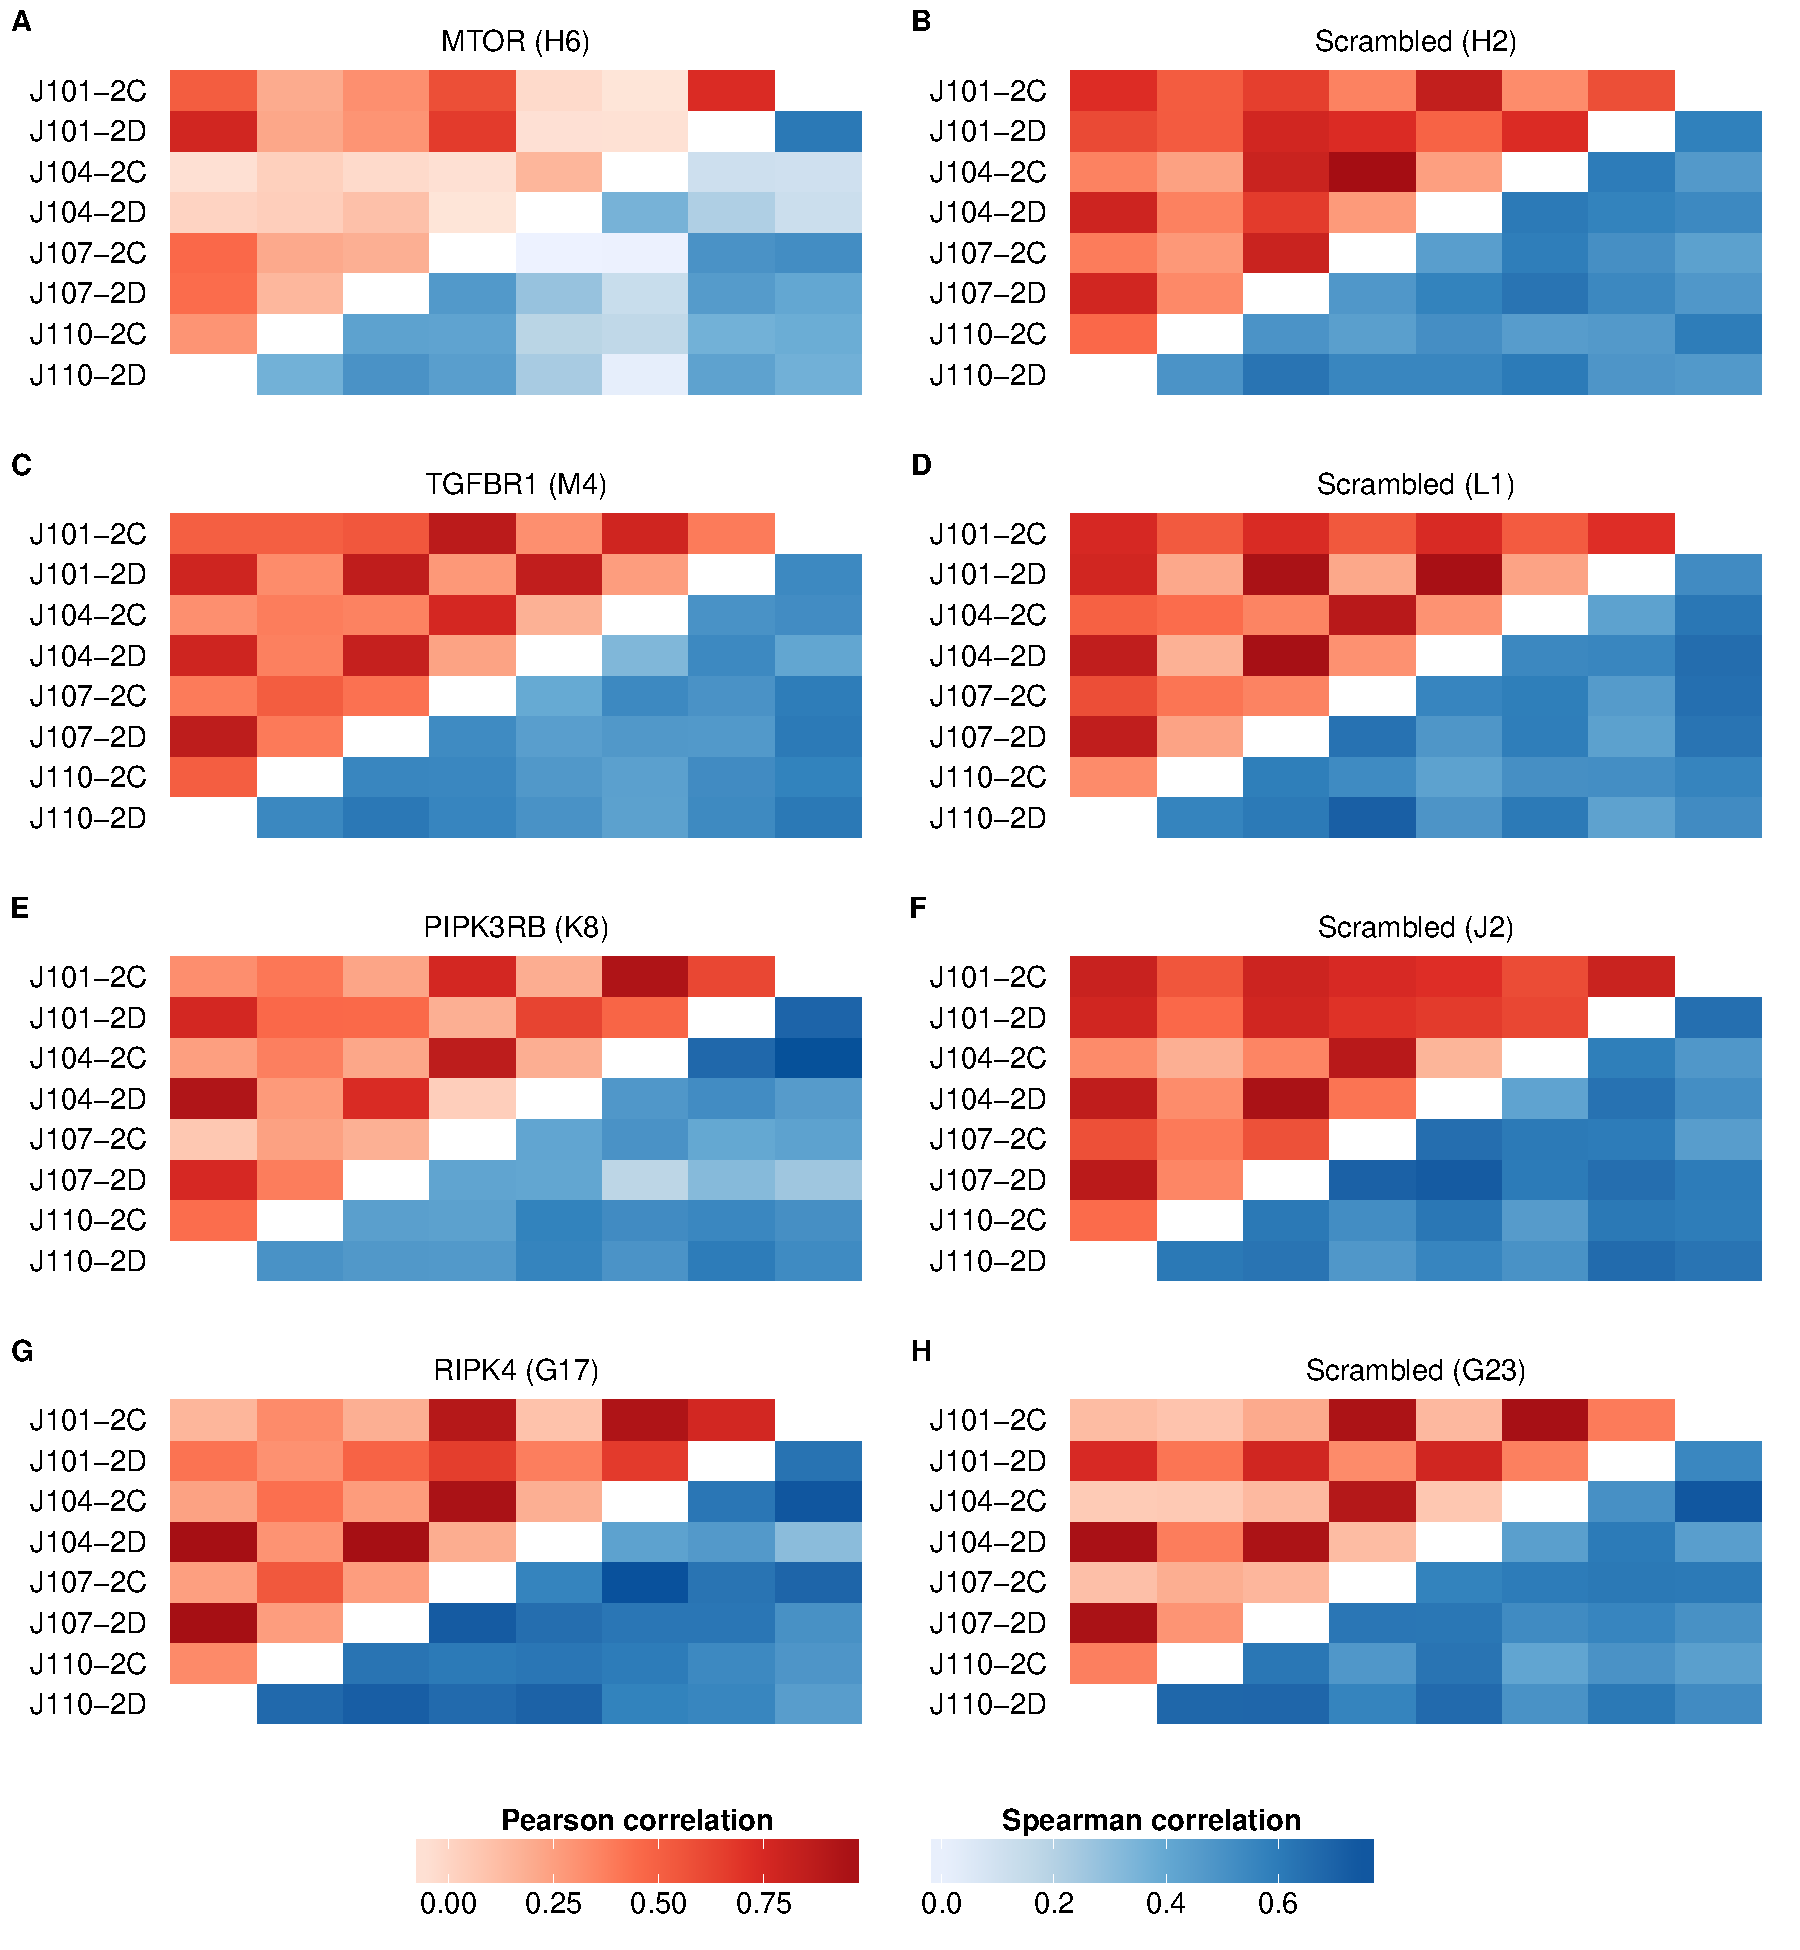
\includegraphics[width=\maxwidth]{figures/R/forest-corr-forest-corr-1} 

}

\caption[Heatmap representations of Pearson and Spearman correlation among feature importance scores obtained by random forest analysis.]{Heatmap representations of correlation matrices obtained by comparing importance scores of features as determined by random forest analysis. Red shades indicate Pearson correlation while blue shades visualize Spearman's rank correlation coefficients. For each gene and scrambled well, all available 8 replicates of the \textit{Brucella} Dharmacon unpooled dataset were considered.}\label{fig:forest-corr}
\end{figure}


\end{knitrout}



%%% Local Variables: 
%%% mode: latex
%%% TeX-master: "00_Master"
%%% End: 


%%%%%%%%%%%%%%%%%%%%%%%%%%%%%%%%%%%%%%%%%%%%%%%%%%%%%%%%%%%%%%%%%%%%%%%%%%%%%%%
%%%  Declaration of originality                                             %%%
%%%%%%%%%%%%%%%%%%%%%%%%%%%%%%%%%%%%%%%%%%%%%%%%%%%%%%%%%%%%%%%%%%%%%%%%%%%%%%%

\cleartorecto
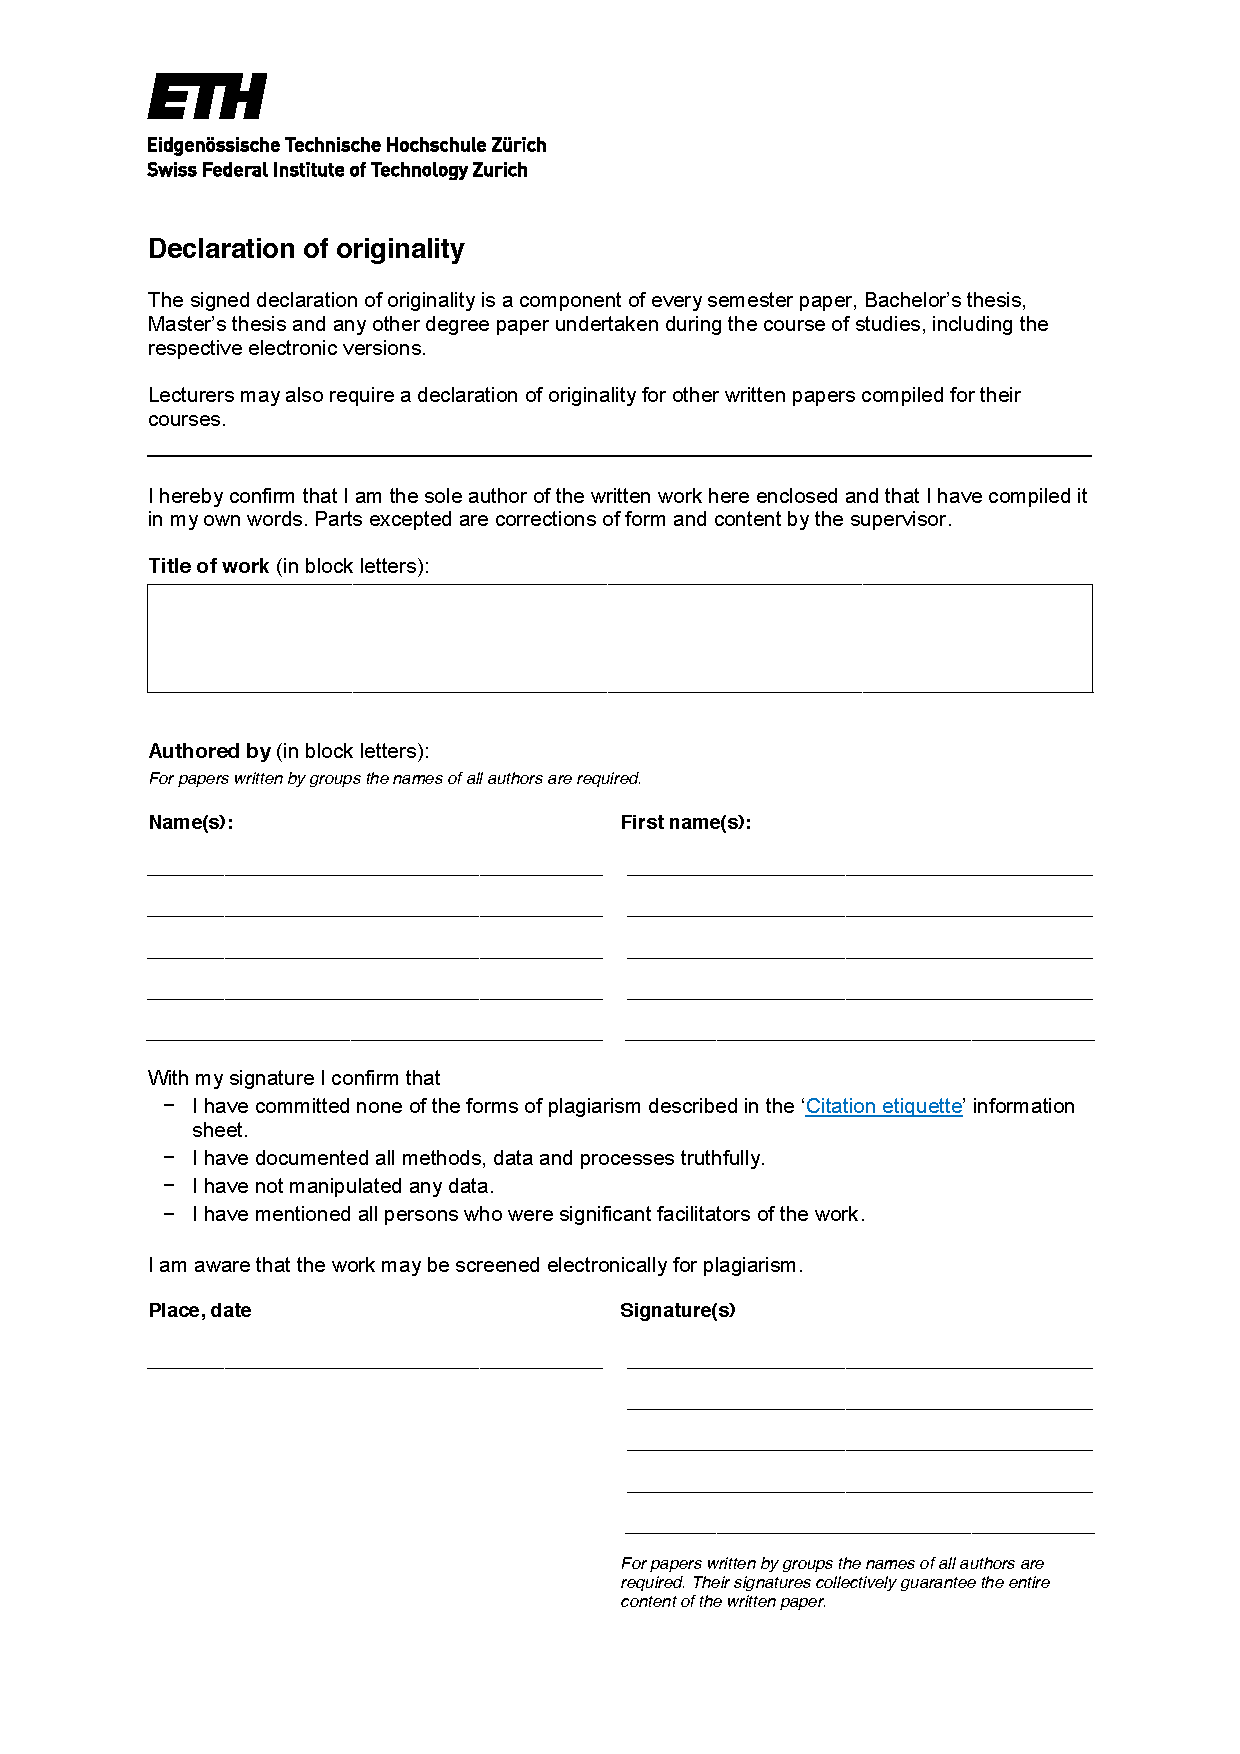
\includepdf[pages={-}]{declaration-originality.pdf}

\end{document}
